\section{Full cell results}
\label{app:cells}

Table~\ref{tab:percell} contains every development factor cell for the
release checkpoint and every registered adaptation run. Entries are generated
directly from the copied report receipt; no unsuccessful run or cell is removed.
Percentages in these tables use decimal half-up rounding to two places;
retention decisions use the unrounded recorded values. These are point-estimate tables. The accompanying machine-readable report also
contains the registered paired intervals and gained/lost counts; no between-arm
interval is claimed by the plotted seed spread.

\begingroup\small
\setlength{\tabcolsep}{4pt}
\begin{longtable}{l>{\raggedright\arraybackslash}p{.42\linewidth}rrr}
\caption{Complete development cell results for the release and each adaptation run.}\label{tab:percell}\\
\toprule
Run & % receipt: evidence/tools/reports/paper/lora_curve_2026-09-10/lora_report.complete.json; source: evidence/tools/reports/paper/lora_curve_2026-09-10/lora_report.json; column definitions
Cell / convention & % receipt: evidence/tools/reports/paper/lora_curve_2026-09-10/lora_report.complete.json; source: evidence/tools/reports/paper/lora_curve_2026-09-10/lora_report.json; column definitions
N & % receipt: evidence/tools/reports/paper/lora_curve_2026-09-10/lora_report.complete.json; source: evidence/tools/reports/paper/lora_curve_2026-09-10/lora_report.json; column definitions
Exact (\%) & % receipt: evidence/tools/reports/paper/lora_curve_2026-09-10/lora_report.complete.json; source: evidence/tools/reports/paper/lora_curve_2026-09-10/lora_report.json; column definitions
Square (\%) \\ % receipt: evidence/tools/reports/paper/lora_curve_2026-09-10/lora_report.complete.json; source: evidence/tools/reports/paper/lora_curve_2026-09-10/lora_report.json; column definitions
\midrule

\endfirsthead
\toprule
Run & % receipt: evidence/tools/reports/paper/lora_curve_2026-09-10/lora_report.complete.json; source: evidence/tools/reports/paper/lora_curve_2026-09-10/lora_report.json; column definitions
Cell / convention & % receipt: evidence/tools/reports/paper/lora_curve_2026-09-10/lora_report.complete.json; source: evidence/tools/reports/paper/lora_curve_2026-09-10/lora_report.json; column definitions
N & % receipt: evidence/tools/reports/paper/lora_curve_2026-09-10/lora_report.complete.json; source: evidence/tools/reports/paper/lora_curve_2026-09-10/lora_report.json; column definitions
Exact (\%) & % receipt: evidence/tools/reports/paper/lora_curve_2026-09-10/lora_report.complete.json; source: evidence/tools/reports/paper/lora_curve_2026-09-10/lora_report.json; column definitions
Square (\%) \\ % receipt: evidence/tools/reports/paper/lora_curve_2026-09-10/lora_report.complete.json; source: evidence/tools/reports/paper/lora_curve_2026-09-10/lora_report.json; column definitions
\midrule

\endhead
\bottomrule\endfoot
release & % receipt: evidence/tools/reports/paper/lora_curve_2026-09-10/lora_report.complete.json; source: evidence/tools/reports/paper/lora_curve_2026-09-10/lora_report.json; release/metrics/dev/by_factor_cell_parity/elevation:08_15/a1_dark
elevation:08\_\allowbreak{}15/dark & % receipt: evidence/tools/reports/paper/lora_curve_2026-09-10/lora_report.complete.json; source: evidence/tools/reports/paper/lora_curve_2026-09-10/lora_report.json; release/metrics/dev/by_factor_cell_parity/elevation:08_15/a1_dark
400 & % receipt: evidence/tools/reports/paper/lora_curve_2026-09-10/lora_report.complete.json; source: evidence/tools/reports/paper/lora_curve_2026-09-10/lora_report.json; release/metrics/dev/by_factor_cell_parity/elevation:08_15/a1_dark
0.00 & % receipt: evidence/tools/reports/paper/lora_curve_2026-09-10/lora_report.complete.json; source: evidence/tools/reports/paper/lora_curve_2026-09-10/lora_report.json; release/metrics/dev/by_factor_cell_parity/elevation:08_15/a1_dark
75.04 \\ % receipt: evidence/tools/reports/paper/lora_curve_2026-09-10/lora_report.complete.json; source: evidence/tools/reports/paper/lora_curve_2026-09-10/lora_report.json; release/metrics/dev/by_factor_cell_parity/elevation:08_15/a1_dark

release & % receipt: evidence/tools/reports/paper/lora_curve_2026-09-10/lora_report.complete.json; source: evidence/tools/reports/paper/lora_curve_2026-09-10/lora_report.json; release/metrics/dev/by_factor_cell_parity/elevation:08_15/a1_light
elevation:08\_\allowbreak{}15/light & % receipt: evidence/tools/reports/paper/lora_curve_2026-09-10/lora_report.complete.json; source: evidence/tools/reports/paper/lora_curve_2026-09-10/lora_report.json; release/metrics/dev/by_factor_cell_parity/elevation:08_15/a1_light
400 & % receipt: evidence/tools/reports/paper/lora_curve_2026-09-10/lora_report.complete.json; source: evidence/tools/reports/paper/lora_curve_2026-09-10/lora_report.json; release/metrics/dev/by_factor_cell_parity/elevation:08_15/a1_light
0.00 & % receipt: evidence/tools/reports/paper/lora_curve_2026-09-10/lora_report.complete.json; source: evidence/tools/reports/paper/lora_curve_2026-09-10/lora_report.json; release/metrics/dev/by_factor_cell_parity/elevation:08_15/a1_light
57.89 \\ % receipt: evidence/tools/reports/paper/lora_curve_2026-09-10/lora_report.complete.json; source: evidence/tools/reports/paper/lora_curve_2026-09-10/lora_report.json; release/metrics/dev/by_factor_cell_parity/elevation:08_15/a1_light

release & % receipt: evidence/tools/reports/paper/lora_curve_2026-09-10/lora_report.complete.json; source: evidence/tools/reports/paper/lora_curve_2026-09-10/lora_report.json; release/metrics/dev/by_factor_cell_parity/elevation:15_25/a1_dark
elevation:15\_\allowbreak{}25/dark & % receipt: evidence/tools/reports/paper/lora_curve_2026-09-10/lora_report.complete.json; source: evidence/tools/reports/paper/lora_curve_2026-09-10/lora_report.json; release/metrics/dev/by_factor_cell_parity/elevation:15_25/a1_dark
400 & % receipt: evidence/tools/reports/paper/lora_curve_2026-09-10/lora_report.complete.json; source: evidence/tools/reports/paper/lora_curve_2026-09-10/lora_report.json; release/metrics/dev/by_factor_cell_parity/elevation:15_25/a1_dark
5.75 & % receipt: evidence/tools/reports/paper/lora_curve_2026-09-10/lora_report.complete.json; source: evidence/tools/reports/paper/lora_curve_2026-09-10/lora_report.json; release/metrics/dev/by_factor_cell_parity/elevation:15_25/a1_dark
88.21 \\ % receipt: evidence/tools/reports/paper/lora_curve_2026-09-10/lora_report.complete.json; source: evidence/tools/reports/paper/lora_curve_2026-09-10/lora_report.json; release/metrics/dev/by_factor_cell_parity/elevation:15_25/a1_dark

release & % receipt: evidence/tools/reports/paper/lora_curve_2026-09-10/lora_report.complete.json; source: evidence/tools/reports/paper/lora_curve_2026-09-10/lora_report.json; release/metrics/dev/by_factor_cell_parity/elevation:15_25/a1_light
elevation:15\_\allowbreak{}25/light & % receipt: evidence/tools/reports/paper/lora_curve_2026-09-10/lora_report.complete.json; source: evidence/tools/reports/paper/lora_curve_2026-09-10/lora_report.json; release/metrics/dev/by_factor_cell_parity/elevation:15_25/a1_light
400 & % receipt: evidence/tools/reports/paper/lora_curve_2026-09-10/lora_report.complete.json; source: evidence/tools/reports/paper/lora_curve_2026-09-10/lora_report.json; release/metrics/dev/by_factor_cell_parity/elevation:15_25/a1_light
0.00 & % receipt: evidence/tools/reports/paper/lora_curve_2026-09-10/lora_report.complete.json; source: evidence/tools/reports/paper/lora_curve_2026-09-10/lora_report.json; release/metrics/dev/by_factor_cell_parity/elevation:15_25/a1_light
56.19 \\ % receipt: evidence/tools/reports/paper/lora_curve_2026-09-10/lora_report.complete.json; source: evidence/tools/reports/paper/lora_curve_2026-09-10/lora_report.json; release/metrics/dev/by_factor_cell_parity/elevation:15_25/a1_light

release & % receipt: evidence/tools/reports/paper/lora_curve_2026-09-10/lora_report.complete.json; source: evidence/tools/reports/paper/lora_curve_2026-09-10/lora_report.json; release/metrics/dev/by_factor_cell_parity/elevation:25_45/a1_dark
elevation:25\_\allowbreak{}45/dark & % receipt: evidence/tools/reports/paper/lora_curve_2026-09-10/lora_report.complete.json; source: evidence/tools/reports/paper/lora_curve_2026-09-10/lora_report.json; release/metrics/dev/by_factor_cell_parity/elevation:25_45/a1_dark
400 & % receipt: evidence/tools/reports/paper/lora_curve_2026-09-10/lora_report.complete.json; source: evidence/tools/reports/paper/lora_curve_2026-09-10/lora_report.json; release/metrics/dev/by_factor_cell_parity/elevation:25_45/a1_dark
18.00 & % receipt: evidence/tools/reports/paper/lora_curve_2026-09-10/lora_report.complete.json; source: evidence/tools/reports/paper/lora_curve_2026-09-10/lora_report.json; release/metrics/dev/by_factor_cell_parity/elevation:25_45/a1_dark
87.28 \\ % receipt: evidence/tools/reports/paper/lora_curve_2026-09-10/lora_report.complete.json; source: evidence/tools/reports/paper/lora_curve_2026-09-10/lora_report.json; release/metrics/dev/by_factor_cell_parity/elevation:25_45/a1_dark

release & % receipt: evidence/tools/reports/paper/lora_curve_2026-09-10/lora_report.complete.json; source: evidence/tools/reports/paper/lora_curve_2026-09-10/lora_report.json; release/metrics/dev/by_factor_cell_parity/elevation:25_45/a1_light
elevation:25\_\allowbreak{}45/light & % receipt: evidence/tools/reports/paper/lora_curve_2026-09-10/lora_report.complete.json; source: evidence/tools/reports/paper/lora_curve_2026-09-10/lora_report.json; release/metrics/dev/by_factor_cell_parity/elevation:25_45/a1_light
400 & % receipt: evidence/tools/reports/paper/lora_curve_2026-09-10/lora_report.complete.json; source: evidence/tools/reports/paper/lora_curve_2026-09-10/lora_report.json; release/metrics/dev/by_factor_cell_parity/elevation:25_45/a1_light
0.00 & % receipt: evidence/tools/reports/paper/lora_curve_2026-09-10/lora_report.complete.json; source: evidence/tools/reports/paper/lora_curve_2026-09-10/lora_report.json; release/metrics/dev/by_factor_cell_parity/elevation:25_45/a1_light
53.94 \\ % receipt: evidence/tools/reports/paper/lora_curve_2026-09-10/lora_report.complete.json; source: evidence/tools/reports/paper/lora_curve_2026-09-10/lora_report.json; release/metrics/dev/by_factor_cell_parity/elevation:25_45/a1_light

release & % receipt: evidence/tools/reports/paper/lora_curve_2026-09-10/lora_report.complete.json; source: evidence/tools/reports/paper/lora_curve_2026-09-10/lora_report.json; release/metrics/dev/by_factor_cell_parity/elevation:45_60/a1_dark
elevation:45\_\allowbreak{}60/dark & % receipt: evidence/tools/reports/paper/lora_curve_2026-09-10/lora_report.complete.json; source: evidence/tools/reports/paper/lora_curve_2026-09-10/lora_report.json; release/metrics/dev/by_factor_cell_parity/elevation:45_60/a1_dark
400 & % receipt: evidence/tools/reports/paper/lora_curve_2026-09-10/lora_report.complete.json; source: evidence/tools/reports/paper/lora_curve_2026-09-10/lora_report.json; release/metrics/dev/by_factor_cell_parity/elevation:45_60/a1_dark
14.25 & % receipt: evidence/tools/reports/paper/lora_curve_2026-09-10/lora_report.complete.json; source: evidence/tools/reports/paper/lora_curve_2026-09-10/lora_report.json; release/metrics/dev/by_factor_cell_parity/elevation:45_60/a1_dark
84.19 \\ % receipt: evidence/tools/reports/paper/lora_curve_2026-09-10/lora_report.complete.json; source: evidence/tools/reports/paper/lora_curve_2026-09-10/lora_report.json; release/metrics/dev/by_factor_cell_parity/elevation:45_60/a1_dark

release & % receipt: evidence/tools/reports/paper/lora_curve_2026-09-10/lora_report.complete.json; source: evidence/tools/reports/paper/lora_curve_2026-09-10/lora_report.json; release/metrics/dev/by_factor_cell_parity/elevation:45_60/a1_light
elevation:45\_\allowbreak{}60/light & % receipt: evidence/tools/reports/paper/lora_curve_2026-09-10/lora_report.complete.json; source: evidence/tools/reports/paper/lora_curve_2026-09-10/lora_report.json; release/metrics/dev/by_factor_cell_parity/elevation:45_60/a1_light
400 & % receipt: evidence/tools/reports/paper/lora_curve_2026-09-10/lora_report.complete.json; source: evidence/tools/reports/paper/lora_curve_2026-09-10/lora_report.json; release/metrics/dev/by_factor_cell_parity/elevation:45_60/a1_light
0.00 & % receipt: evidence/tools/reports/paper/lora_curve_2026-09-10/lora_report.complete.json; source: evidence/tools/reports/paper/lora_curve_2026-09-10/lora_report.json; release/metrics/dev/by_factor_cell_parity/elevation:45_60/a1_light
52.89 \\ % receipt: evidence/tools/reports/paper/lora_curve_2026-09-10/lora_report.complete.json; source: evidence/tools/reports/paper/lora_curve_2026-09-10/lora_report.json; release/metrics/dev/by_factor_cell_parity/elevation:45_60/a1_light

release & % receipt: evidence/tools/reports/paper/lora_curve_2026-09-10/lora_report.complete.json; source: evidence/tools/reports/paper/lora_curve_2026-09-10/lora_report.json; release/metrics/dev/by_factor_cell_parity/framing:compact/a1_dark
framing:compact/dark & % receipt: evidence/tools/reports/paper/lora_curve_2026-09-10/lora_report.complete.json; source: evidence/tools/reports/paper/lora_curve_2026-09-10/lora_report.json; release/metrics/dev/by_factor_cell_parity/framing:compact/a1_dark
400 & % receipt: evidence/tools/reports/paper/lora_curve_2026-09-10/lora_report.complete.json; source: evidence/tools/reports/paper/lora_curve_2026-09-10/lora_report.json; release/metrics/dev/by_factor_cell_parity/framing:compact/a1_dark
7.25 & % receipt: evidence/tools/reports/paper/lora_curve_2026-09-10/lora_report.complete.json; source: evidence/tools/reports/paper/lora_curve_2026-09-10/lora_report.json; release/metrics/dev/by_factor_cell_parity/framing:compact/a1_dark
85.01 \\ % receipt: evidence/tools/reports/paper/lora_curve_2026-09-10/lora_report.complete.json; source: evidence/tools/reports/paper/lora_curve_2026-09-10/lora_report.json; release/metrics/dev/by_factor_cell_parity/framing:compact/a1_dark

release & % receipt: evidence/tools/reports/paper/lora_curve_2026-09-10/lora_report.complete.json; source: evidence/tools/reports/paper/lora_curve_2026-09-10/lora_report.json; release/metrics/dev/by_factor_cell_parity/framing:compact/a1_light
framing:compact/light & % receipt: evidence/tools/reports/paper/lora_curve_2026-09-10/lora_report.complete.json; source: evidence/tools/reports/paper/lora_curve_2026-09-10/lora_report.json; release/metrics/dev/by_factor_cell_parity/framing:compact/a1_light
400 & % receipt: evidence/tools/reports/paper/lora_curve_2026-09-10/lora_report.complete.json; source: evidence/tools/reports/paper/lora_curve_2026-09-10/lora_report.json; release/metrics/dev/by_factor_cell_parity/framing:compact/a1_light
0.00 & % receipt: evidence/tools/reports/paper/lora_curve_2026-09-10/lora_report.complete.json; source: evidence/tools/reports/paper/lora_curve_2026-09-10/lora_report.json; release/metrics/dev/by_factor_cell_parity/framing:compact/a1_light
52.18 \\ % receipt: evidence/tools/reports/paper/lora_curve_2026-09-10/lora_report.complete.json; source: evidence/tools/reports/paper/lora_curve_2026-09-10/lora_report.json; release/metrics/dev/by_factor_cell_parity/framing:compact/a1_light

release & % receipt: evidence/tools/reports/paper/lora_curve_2026-09-10/lora_report.complete.json; source: evidence/tools/reports/paper/lora_curve_2026-09-10/lora_report.json; release/metrics/dev/by_factor_cell_parity/framing:standard/a1_dark
framing:standard/dark & % receipt: evidence/tools/reports/paper/lora_curve_2026-09-10/lora_report.complete.json; source: evidence/tools/reports/paper/lora_curve_2026-09-10/lora_report.json; release/metrics/dev/by_factor_cell_parity/framing:standard/a1_dark
400 & % receipt: evidence/tools/reports/paper/lora_curve_2026-09-10/lora_report.complete.json; source: evidence/tools/reports/paper/lora_curve_2026-09-10/lora_report.json; release/metrics/dev/by_factor_cell_parity/framing:standard/a1_dark
14.25 & % receipt: evidence/tools/reports/paper/lora_curve_2026-09-10/lora_report.complete.json; source: evidence/tools/reports/paper/lora_curve_2026-09-10/lora_report.json; release/metrics/dev/by_factor_cell_parity/framing:standard/a1_dark
84.19 \\ % receipt: evidence/tools/reports/paper/lora_curve_2026-09-10/lora_report.complete.json; source: evidence/tools/reports/paper/lora_curve_2026-09-10/lora_report.json; release/metrics/dev/by_factor_cell_parity/framing:standard/a1_dark

release & % receipt: evidence/tools/reports/paper/lora_curve_2026-09-10/lora_report.complete.json; source: evidence/tools/reports/paper/lora_curve_2026-09-10/lora_report.json; release/metrics/dev/by_factor_cell_parity/framing:standard/a1_light
framing:standard/light & % receipt: evidence/tools/reports/paper/lora_curve_2026-09-10/lora_report.complete.json; source: evidence/tools/reports/paper/lora_curve_2026-09-10/lora_report.json; release/metrics/dev/by_factor_cell_parity/framing:standard/a1_light
400 & % receipt: evidence/tools/reports/paper/lora_curve_2026-09-10/lora_report.complete.json; source: evidence/tools/reports/paper/lora_curve_2026-09-10/lora_report.json; release/metrics/dev/by_factor_cell_parity/framing:standard/a1_light
0.00 & % receipt: evidence/tools/reports/paper/lora_curve_2026-09-10/lora_report.complete.json; source: evidence/tools/reports/paper/lora_curve_2026-09-10/lora_report.json; release/metrics/dev/by_factor_cell_parity/framing:standard/a1_light
52.89 \\ % receipt: evidence/tools/reports/paper/lora_curve_2026-09-10/lora_report.complete.json; source: evidence/tools/reports/paper/lora_curve_2026-09-10/lora_report.json; release/metrics/dev/by_factor_cell_parity/framing:standard/a1_light

release & % receipt: evidence/tools/reports/paper/lora_curve_2026-09-10/lora_report.complete.json; source: evidence/tools/reports/paper/lora_curve_2026-09-10/lora_report.json; release/metrics/dev/by_factor_cell_parity/geometry:deplorable/a1_dark
geometry:deplorable/dark & % receipt: evidence/tools/reports/paper/lora_curve_2026-09-10/lora_report.complete.json; source: evidence/tools/reports/paper/lora_curve_2026-09-10/lora_report.json; release/metrics/dev/by_factor_cell_parity/geometry:deplorable/a1_dark
400 & % receipt: evidence/tools/reports/paper/lora_curve_2026-09-10/lora_report.complete.json; source: evidence/tools/reports/paper/lora_curve_2026-09-10/lora_report.json; release/metrics/dev/by_factor_cell_parity/geometry:deplorable/a1_dark
34.25 & % receipt: evidence/tools/reports/paper/lora_curve_2026-09-10/lora_report.complete.json; source: evidence/tools/reports/paper/lora_curve_2026-09-10/lora_report.json; release/metrics/dev/by_factor_cell_parity/geometry:deplorable/a1_dark
86.95 \\ % receipt: evidence/tools/reports/paper/lora_curve_2026-09-10/lora_report.complete.json; source: evidence/tools/reports/paper/lora_curve_2026-09-10/lora_report.json; release/metrics/dev/by_factor_cell_parity/geometry:deplorable/a1_dark

release & % receipt: evidence/tools/reports/paper/lora_curve_2026-09-10/lora_report.complete.json; source: evidence/tools/reports/paper/lora_curve_2026-09-10/lora_report.json; release/metrics/dev/by_factor_cell_parity/geometry:deplorable/a1_light
geometry:deplorable/light & % receipt: evidence/tools/reports/paper/lora_curve_2026-09-10/lora_report.complete.json; source: evidence/tools/reports/paper/lora_curve_2026-09-10/lora_report.json; release/metrics/dev/by_factor_cell_parity/geometry:deplorable/a1_light
400 & % receipt: evidence/tools/reports/paper/lora_curve_2026-09-10/lora_report.complete.json; source: evidence/tools/reports/paper/lora_curve_2026-09-10/lora_report.json; release/metrics/dev/by_factor_cell_parity/geometry:deplorable/a1_light
0.00 & % receipt: evidence/tools/reports/paper/lora_curve_2026-09-10/lora_report.complete.json; source: evidence/tools/reports/paper/lora_curve_2026-09-10/lora_report.json; release/metrics/dev/by_factor_cell_parity/geometry:deplorable/a1_light
53.63 \\ % receipt: evidence/tools/reports/paper/lora_curve_2026-09-10/lora_report.complete.json; source: evidence/tools/reports/paper/lora_curve_2026-09-10/lora_report.json; release/metrics/dev/by_factor_cell_parity/geometry:deplorable/a1_light

release & % receipt: evidence/tools/reports/paper/lora_curve_2026-09-10/lora_report.complete.json; source: evidence/tools/reports/paper/lora_curve_2026-09-10/lora_report.json; release/metrics/dev/by_factor_cell_parity/geometry:killgorack/a1_dark
geometry:killgorack/dark & % receipt: evidence/tools/reports/paper/lora_curve_2026-09-10/lora_report.complete.json; source: evidence/tools/reports/paper/lora_curve_2026-09-10/lora_report.json; release/metrics/dev/by_factor_cell_parity/geometry:killgorack/a1_dark
400 & % receipt: evidence/tools/reports/paper/lora_curve_2026-09-10/lora_report.complete.json; source: evidence/tools/reports/paper/lora_curve_2026-09-10/lora_report.json; release/metrics/dev/by_factor_cell_parity/geometry:killgorack/a1_dark
25.75 & % receipt: evidence/tools/reports/paper/lora_curve_2026-09-10/lora_report.complete.json; source: evidence/tools/reports/paper/lora_curve_2026-09-10/lora_report.json; release/metrics/dev/by_factor_cell_parity/geometry:killgorack/a1_dark
85.27 \\ % receipt: evidence/tools/reports/paper/lora_curve_2026-09-10/lora_report.complete.json; source: evidence/tools/reports/paper/lora_curve_2026-09-10/lora_report.json; release/metrics/dev/by_factor_cell_parity/geometry:killgorack/a1_dark

release & % receipt: evidence/tools/reports/paper/lora_curve_2026-09-10/lora_report.complete.json; source: evidence/tools/reports/paper/lora_curve_2026-09-10/lora_report.json; release/metrics/dev/by_factor_cell_parity/geometry:killgorack/a1_light
geometry:killgorack/light & % receipt: evidence/tools/reports/paper/lora_curve_2026-09-10/lora_report.complete.json; source: evidence/tools/reports/paper/lora_curve_2026-09-10/lora_report.json; release/metrics/dev/by_factor_cell_parity/geometry:killgorack/a1_light
400 & % receipt: evidence/tools/reports/paper/lora_curve_2026-09-10/lora_report.complete.json; source: evidence/tools/reports/paper/lora_curve_2026-09-10/lora_report.json; release/metrics/dev/by_factor_cell_parity/geometry:killgorack/a1_light
0.00 & % receipt: evidence/tools/reports/paper/lora_curve_2026-09-10/lora_report.complete.json; source: evidence/tools/reports/paper/lora_curve_2026-09-10/lora_report.json; release/metrics/dev/by_factor_cell_parity/geometry:killgorack/a1_light
53.81 \\ % receipt: evidence/tools/reports/paper/lora_curve_2026-09-10/lora_report.complete.json; source: evidence/tools/reports/paper/lora_curve_2026-09-10/lora_report.json; release/metrics/dev/by_factor_cell_parity/geometry:killgorack/a1_light

release & % receipt: evidence/tools/reports/paper/lora_curve_2026-09-10/lora_report.complete.json; source: evidence/tools/reports/paper/lora_curve_2026-09-10/lora_report.json; release/metrics/dev/by_factor_cell_parity/geometry:lyricsz/a1_dark
geometry:lyricsz/dark & % receipt: evidence/tools/reports/paper/lora_curve_2026-09-10/lora_report.complete.json; source: evidence/tools/reports/paper/lora_curve_2026-09-10/lora_report.json; release/metrics/dev/by_factor_cell_parity/geometry:lyricsz/a1_dark
400 & % receipt: evidence/tools/reports/paper/lora_curve_2026-09-10/lora_report.complete.json; source: evidence/tools/reports/paper/lora_curve_2026-09-10/lora_report.json; release/metrics/dev/by_factor_cell_parity/geometry:lyricsz/a1_dark
3.00 & % receipt: evidence/tools/reports/paper/lora_curve_2026-09-10/lora_report.complete.json; source: evidence/tools/reports/paper/lora_curve_2026-09-10/lora_report.json; release/metrics/dev/by_factor_cell_parity/geometry:lyricsz/a1_dark
83.43 \\ % receipt: evidence/tools/reports/paper/lora_curve_2026-09-10/lora_report.complete.json; source: evidence/tools/reports/paper/lora_curve_2026-09-10/lora_report.json; release/metrics/dev/by_factor_cell_parity/geometry:lyricsz/a1_dark

release & % receipt: evidence/tools/reports/paper/lora_curve_2026-09-10/lora_report.complete.json; source: evidence/tools/reports/paper/lora_curve_2026-09-10/lora_report.json; release/metrics/dev/by_factor_cell_parity/geometry:lyricsz/a1_light
geometry:lyricsz/light & % receipt: evidence/tools/reports/paper/lora_curve_2026-09-10/lora_report.complete.json; source: evidence/tools/reports/paper/lora_curve_2026-09-10/lora_report.json; release/metrics/dev/by_factor_cell_parity/geometry:lyricsz/a1_light
400 & % receipt: evidence/tools/reports/paper/lora_curve_2026-09-10/lora_report.complete.json; source: evidence/tools/reports/paper/lora_curve_2026-09-10/lora_report.json; release/metrics/dev/by_factor_cell_parity/geometry:lyricsz/a1_light
0.00 & % receipt: evidence/tools/reports/paper/lora_curve_2026-09-10/lora_report.complete.json; source: evidence/tools/reports/paper/lora_curve_2026-09-10/lora_report.json; release/metrics/dev/by_factor_cell_parity/geometry:lyricsz/a1_light
55.74 \\ % receipt: evidence/tools/reports/paper/lora_curve_2026-09-10/lora_report.complete.json; source: evidence/tools/reports/paper/lora_curve_2026-09-10/lora_report.json; release/metrics/dev/by_factor_cell_parity/geometry:lyricsz/a1_light

release & % receipt: evidence/tools/reports/paper/lora_curve_2026-09-10/lora_report.complete.json; source: evidence/tools/reports/paper/lora_curve_2026-09-10/lora_report.json; release/metrics/dev/by_factor_cell_parity/geometry:nailfighter/a1_dark
geometry:nailfighter/dark & % receipt: evidence/tools/reports/paper/lora_curve_2026-09-10/lora_report.complete.json; source: evidence/tools/reports/paper/lora_curve_2026-09-10/lora_report.json; release/metrics/dev/by_factor_cell_parity/geometry:nailfighter/a1_dark
400 & % receipt: evidence/tools/reports/paper/lora_curve_2026-09-10/lora_report.complete.json; source: evidence/tools/reports/paper/lora_curve_2026-09-10/lora_report.json; release/metrics/dev/by_factor_cell_parity/geometry:nailfighter/a1_dark
25.00 & % receipt: evidence/tools/reports/paper/lora_curve_2026-09-10/lora_report.complete.json; source: evidence/tools/reports/paper/lora_curve_2026-09-10/lora_report.json; release/metrics/dev/by_factor_cell_parity/geometry:nailfighter/a1_dark
87.52 \\ % receipt: evidence/tools/reports/paper/lora_curve_2026-09-10/lora_report.complete.json; source: evidence/tools/reports/paper/lora_curve_2026-09-10/lora_report.json; release/metrics/dev/by_factor_cell_parity/geometry:nailfighter/a1_dark

release & % receipt: evidence/tools/reports/paper/lora_curve_2026-09-10/lora_report.complete.json; source: evidence/tools/reports/paper/lora_curve_2026-09-10/lora_report.json; release/metrics/dev/by_factor_cell_parity/geometry:nailfighter/a1_light
geometry:nailfighter/light & % receipt: evidence/tools/reports/paper/lora_curve_2026-09-10/lora_report.complete.json; source: evidence/tools/reports/paper/lora_curve_2026-09-10/lora_report.json; release/metrics/dev/by_factor_cell_parity/geometry:nailfighter/a1_light
400 & % receipt: evidence/tools/reports/paper/lora_curve_2026-09-10/lora_report.complete.json; source: evidence/tools/reports/paper/lora_curve_2026-09-10/lora_report.json; release/metrics/dev/by_factor_cell_parity/geometry:nailfighter/a1_light
0.00 & % receipt: evidence/tools/reports/paper/lora_curve_2026-09-10/lora_report.complete.json; source: evidence/tools/reports/paper/lora_curve_2026-09-10/lora_report.json; release/metrics/dev/by_factor_cell_parity/geometry:nailfighter/a1_light
54.04 \\ % receipt: evidence/tools/reports/paper/lora_curve_2026-09-10/lora_report.complete.json; source: evidence/tools/reports/paper/lora_curve_2026-09-10/lora_report.json; release/metrics/dev/by_factor_cell_parity/geometry:nailfighter/a1_light

release & % receipt: evidence/tools/reports/paper/lora_curve_2026-09-10/lora_report.complete.json; source: evidence/tools/reports/paper/lora_curve_2026-09-10/lora_report.json; release/metrics/dev/by_factor_cell_parity/geometry:omie/a1_dark
geometry:omie/dark & % receipt: evidence/tools/reports/paper/lora_curve_2026-09-10/lora_report.complete.json; source: evidence/tools/reports/paper/lora_curve_2026-09-10/lora_report.json; release/metrics/dev/by_factor_cell_parity/geometry:omie/a1_dark
400 & % receipt: evidence/tools/reports/paper/lora_curve_2026-09-10/lora_report.complete.json; source: evidence/tools/reports/paper/lora_curve_2026-09-10/lora_report.json; release/metrics/dev/by_factor_cell_parity/geometry:omie/a1_dark
34.25 & % receipt: evidence/tools/reports/paper/lora_curve_2026-09-10/lora_report.complete.json; source: evidence/tools/reports/paper/lora_curve_2026-09-10/lora_report.json; release/metrics/dev/by_factor_cell_parity/geometry:omie/a1_dark
88.35 \\ % receipt: evidence/tools/reports/paper/lora_curve_2026-09-10/lora_report.complete.json; source: evidence/tools/reports/paper/lora_curve_2026-09-10/lora_report.json; release/metrics/dev/by_factor_cell_parity/geometry:omie/a1_dark

release & % receipt: evidence/tools/reports/paper/lora_curve_2026-09-10/lora_report.complete.json; source: evidence/tools/reports/paper/lora_curve_2026-09-10/lora_report.json; release/metrics/dev/by_factor_cell_parity/geometry:omie/a1_light
geometry:omie/light & % receipt: evidence/tools/reports/paper/lora_curve_2026-09-10/lora_report.complete.json; source: evidence/tools/reports/paper/lora_curve_2026-09-10/lora_report.json; release/metrics/dev/by_factor_cell_parity/geometry:omie/a1_light
400 & % receipt: evidence/tools/reports/paper/lora_curve_2026-09-10/lora_report.complete.json; source: evidence/tools/reports/paper/lora_curve_2026-09-10/lora_report.json; release/metrics/dev/by_factor_cell_parity/geometry:omie/a1_light
0.00 & % receipt: evidence/tools/reports/paper/lora_curve_2026-09-10/lora_report.complete.json; source: evidence/tools/reports/paper/lora_curve_2026-09-10/lora_report.json; release/metrics/dev/by_factor_cell_parity/geometry:omie/a1_light
54.60 \\ % receipt: evidence/tools/reports/paper/lora_curve_2026-09-10/lora_report.complete.json; source: evidence/tools/reports/paper/lora_curve_2026-09-10/lora_report.json; release/metrics/dev/by_factor_cell_parity/geometry:omie/a1_light

release & % receipt: evidence/tools/reports/paper/lora_curve_2026-09-10/lora_report.complete.json; source: evidence/tools/reports/paper/lora_curve_2026-09-10/lora_report.json; release/metrics/dev/by_factor_cell_parity/geometry:phuong/a1_dark
geometry:phuong/dark & % receipt: evidence/tools/reports/paper/lora_curve_2026-09-10/lora_report.complete.json; source: evidence/tools/reports/paper/lora_curve_2026-09-10/lora_report.json; release/metrics/dev/by_factor_cell_parity/geometry:phuong/a1_dark
400 & % receipt: evidence/tools/reports/paper/lora_curve_2026-09-10/lora_report.complete.json; source: evidence/tools/reports/paper/lora_curve_2026-09-10/lora_report.json; release/metrics/dev/by_factor_cell_parity/geometry:phuong/a1_dark
17.25 & % receipt: evidence/tools/reports/paper/lora_curve_2026-09-10/lora_report.complete.json; source: evidence/tools/reports/paper/lora_curve_2026-09-10/lora_report.json; release/metrics/dev/by_factor_cell_parity/geometry:phuong/a1_dark
86.04 \\ % receipt: evidence/tools/reports/paper/lora_curve_2026-09-10/lora_report.complete.json; source: evidence/tools/reports/paper/lora_curve_2026-09-10/lora_report.json; release/metrics/dev/by_factor_cell_parity/geometry:phuong/a1_dark

release & % receipt: evidence/tools/reports/paper/lora_curve_2026-09-10/lora_report.complete.json; source: evidence/tools/reports/paper/lora_curve_2026-09-10/lora_report.json; release/metrics/dev/by_factor_cell_parity/geometry:phuong/a1_light
geometry:phuong/light & % receipt: evidence/tools/reports/paper/lora_curve_2026-09-10/lora_report.complete.json; source: evidence/tools/reports/paper/lora_curve_2026-09-10/lora_report.json; release/metrics/dev/by_factor_cell_parity/geometry:phuong/a1_light
400 & % receipt: evidence/tools/reports/paper/lora_curve_2026-09-10/lora_report.complete.json; source: evidence/tools/reports/paper/lora_curve_2026-09-10/lora_report.json; release/metrics/dev/by_factor_cell_parity/geometry:phuong/a1_light
0.00 & % receipt: evidence/tools/reports/paper/lora_curve_2026-09-10/lora_report.complete.json; source: evidence/tools/reports/paper/lora_curve_2026-09-10/lora_report.json; release/metrics/dev/by_factor_cell_parity/geometry:phuong/a1_light
54.87 \\ % receipt: evidence/tools/reports/paper/lora_curve_2026-09-10/lora_report.complete.json; source: evidence/tools/reports/paper/lora_curve_2026-09-10/lora_report.json; release/metrics/dev/by_factor_cell_parity/geometry:phuong/a1_light

release & % receipt: evidence/tools/reports/paper/lora_curve_2026-09-10/lora_report.complete.json; source: evidence/tools/reports/paper/lora_curve_2026-09-10/lora_report.json; release/metrics/dev/by_factor_cell_parity/geometry:pjhanzlik/a1_dark
geometry:pjhanzlik/dark & % receipt: evidence/tools/reports/paper/lora_curve_2026-09-10/lora_report.complete.json; source: evidence/tools/reports/paper/lora_curve_2026-09-10/lora_report.json; release/metrics/dev/by_factor_cell_parity/geometry:pjhanzlik/a1_dark
400 & % receipt: evidence/tools/reports/paper/lora_curve_2026-09-10/lora_report.complete.json; source: evidence/tools/reports/paper/lora_curve_2026-09-10/lora_report.json; release/metrics/dev/by_factor_cell_parity/geometry:pjhanzlik/a1_dark
4.75 & % receipt: evidence/tools/reports/paper/lora_curve_2026-09-10/lora_report.complete.json; source: evidence/tools/reports/paper/lora_curve_2026-09-10/lora_report.json; release/metrics/dev/by_factor_cell_parity/geometry:pjhanzlik/a1_dark
80.97 \\ % receipt: evidence/tools/reports/paper/lora_curve_2026-09-10/lora_report.complete.json; source: evidence/tools/reports/paper/lora_curve_2026-09-10/lora_report.json; release/metrics/dev/by_factor_cell_parity/geometry:pjhanzlik/a1_dark

release & % receipt: evidence/tools/reports/paper/lora_curve_2026-09-10/lora_report.complete.json; source: evidence/tools/reports/paper/lora_curve_2026-09-10/lora_report.json; release/metrics/dev/by_factor_cell_parity/geometry:pjhanzlik/a1_light
geometry:pjhanzlik/light & % receipt: evidence/tools/reports/paper/lora_curve_2026-09-10/lora_report.complete.json; source: evidence/tools/reports/paper/lora_curve_2026-09-10/lora_report.json; release/metrics/dev/by_factor_cell_parity/geometry:pjhanzlik/a1_light
400 & % receipt: evidence/tools/reports/paper/lora_curve_2026-09-10/lora_report.complete.json; source: evidence/tools/reports/paper/lora_curve_2026-09-10/lora_report.json; release/metrics/dev/by_factor_cell_parity/geometry:pjhanzlik/a1_light
0.00 & % receipt: evidence/tools/reports/paper/lora_curve_2026-09-10/lora_report.complete.json; source: evidence/tools/reports/paper/lora_curve_2026-09-10/lora_report.json; release/metrics/dev/by_factor_cell_parity/geometry:pjhanzlik/a1_light
54.66 \\ % receipt: evidence/tools/reports/paper/lora_curve_2026-09-10/lora_report.complete.json; source: evidence/tools/reports/paper/lora_curve_2026-09-10/lora_report.json; release/metrics/dev/by_factor_cell_parity/geometry:pjhanzlik/a1_light

release & % receipt: evidence/tools/reports/paper/lora_curve_2026-09-10/lora_report.complete.json; source: evidence/tools/reports/paper/lora_curve_2026-09-10/lora_report.json; release/metrics/dev/by_factor_cell_parity/geometry:polyhaven/a1_dark
geometry:polyhaven/dark & % receipt: evidence/tools/reports/paper/lora_curve_2026-09-10/lora_report.complete.json; source: evidence/tools/reports/paper/lora_curve_2026-09-10/lora_report.json; release/metrics/dev/by_factor_cell_parity/geometry:polyhaven/a1_dark
400 & % receipt: evidence/tools/reports/paper/lora_curve_2026-09-10/lora_report.complete.json; source: evidence/tools/reports/paper/lora_curve_2026-09-10/lora_report.json; release/metrics/dev/by_factor_cell_parity/geometry:polyhaven/a1_dark
14.25 & % receipt: evidence/tools/reports/paper/lora_curve_2026-09-10/lora_report.complete.json; source: evidence/tools/reports/paper/lora_curve_2026-09-10/lora_report.json; release/metrics/dev/by_factor_cell_parity/geometry:polyhaven/a1_dark
84.19 \\ % receipt: evidence/tools/reports/paper/lora_curve_2026-09-10/lora_report.complete.json; source: evidence/tools/reports/paper/lora_curve_2026-09-10/lora_report.json; release/metrics/dev/by_factor_cell_parity/geometry:polyhaven/a1_dark

release & % receipt: evidence/tools/reports/paper/lora_curve_2026-09-10/lora_report.complete.json; source: evidence/tools/reports/paper/lora_curve_2026-09-10/lora_report.json; release/metrics/dev/by_factor_cell_parity/geometry:polyhaven/a1_light
geometry:polyhaven/light & % receipt: evidence/tools/reports/paper/lora_curve_2026-09-10/lora_report.complete.json; source: evidence/tools/reports/paper/lora_curve_2026-09-10/lora_report.json; release/metrics/dev/by_factor_cell_parity/geometry:polyhaven/a1_light
400 & % receipt: evidence/tools/reports/paper/lora_curve_2026-09-10/lora_report.complete.json; source: evidence/tools/reports/paper/lora_curve_2026-09-10/lora_report.json; release/metrics/dev/by_factor_cell_parity/geometry:polyhaven/a1_light
0.00 & % receipt: evidence/tools/reports/paper/lora_curve_2026-09-10/lora_report.complete.json; source: evidence/tools/reports/paper/lora_curve_2026-09-10/lora_report.json; release/metrics/dev/by_factor_cell_parity/geometry:polyhaven/a1_light
52.89 \\ % receipt: evidence/tools/reports/paper/lora_curve_2026-09-10/lora_report.complete.json; source: evidence/tools/reports/paper/lora_curve_2026-09-10/lora_report.json; release/metrics/dev/by_factor_cell_parity/geometry:polyhaven/a1_light

release & % receipt: evidence/tools/reports/paper/lora_curve_2026-09-10/lora_report.complete.json; source: evidence/tools/reports/paper/lora_curve_2026-09-10/lora_report.json; release/metrics/dev/by_factor_cell_parity/palette:aubergine_periwinkle/a1_dark
palette:aubergine\_\allowbreak{}periwinkle/dark & % receipt: evidence/tools/reports/paper/lora_curve_2026-09-10/lora_report.complete.json; source: evidence/tools/reports/paper/lora_curve_2026-09-10/lora_report.json; release/metrics/dev/by_factor_cell_parity/palette:aubergine_periwinkle/a1_dark
400 & % receipt: evidence/tools/reports/paper/lora_curve_2026-09-10/lora_report.complete.json; source: evidence/tools/reports/paper/lora_curve_2026-09-10/lora_report.json; release/metrics/dev/by_factor_cell_parity/palette:aubergine_periwinkle/a1_dark
14.25 & % receipt: evidence/tools/reports/paper/lora_curve_2026-09-10/lora_report.complete.json; source: evidence/tools/reports/paper/lora_curve_2026-09-10/lora_report.json; release/metrics/dev/by_factor_cell_parity/palette:aubergine_periwinkle/a1_dark
84.75 \\ % receipt: evidence/tools/reports/paper/lora_curve_2026-09-10/lora_report.complete.json; source: evidence/tools/reports/paper/lora_curve_2026-09-10/lora_report.json; release/metrics/dev/by_factor_cell_parity/palette:aubergine_periwinkle/a1_dark

release & % receipt: evidence/tools/reports/paper/lora_curve_2026-09-10/lora_report.complete.json; source: evidence/tools/reports/paper/lora_curve_2026-09-10/lora_report.json; release/metrics/dev/by_factor_cell_parity/palette:aubergine_periwinkle/a1_light
palette:aubergine\_\allowbreak{}periwinkle/light & % receipt: evidence/tools/reports/paper/lora_curve_2026-09-10/lora_report.complete.json; source: evidence/tools/reports/paper/lora_curve_2026-09-10/lora_report.json; release/metrics/dev/by_factor_cell_parity/palette:aubergine_periwinkle/a1_light
400 & % receipt: evidence/tools/reports/paper/lora_curve_2026-09-10/lora_report.complete.json; source: evidence/tools/reports/paper/lora_curve_2026-09-10/lora_report.json; release/metrics/dev/by_factor_cell_parity/palette:aubergine_periwinkle/a1_light
0.00 & % receipt: evidence/tools/reports/paper/lora_curve_2026-09-10/lora_report.complete.json; source: evidence/tools/reports/paper/lora_curve_2026-09-10/lora_report.json; release/metrics/dev/by_factor_cell_parity/palette:aubergine_periwinkle/a1_light
52.86 \\ % receipt: evidence/tools/reports/paper/lora_curve_2026-09-10/lora_report.complete.json; source: evidence/tools/reports/paper/lora_curve_2026-09-10/lora_report.json; release/metrics/dev/by_factor_cell_parity/palette:aubergine_periwinkle/a1_light

release & % receipt: evidence/tools/reports/paper/lora_curve_2026-09-10/lora_report.complete.json; source: evidence/tools/reports/paper/lora_curve_2026-09-10/lora_report.json; release/metrics/dev/by_factor_cell_parity/palette:cobalt_porcelain/a1_dark
palette:cobalt\_\allowbreak{}porcelain/dark & % receipt: evidence/tools/reports/paper/lora_curve_2026-09-10/lora_report.complete.json; source: evidence/tools/reports/paper/lora_curve_2026-09-10/lora_report.json; release/metrics/dev/by_factor_cell_parity/palette:cobalt_porcelain/a1_dark
400 & % receipt: evidence/tools/reports/paper/lora_curve_2026-09-10/lora_report.complete.json; source: evidence/tools/reports/paper/lora_curve_2026-09-10/lora_report.json; release/metrics/dev/by_factor_cell_parity/palette:cobalt_porcelain/a1_dark
13.25 & % receipt: evidence/tools/reports/paper/lora_curve_2026-09-10/lora_report.complete.json; source: evidence/tools/reports/paper/lora_curve_2026-09-10/lora_report.json; release/metrics/dev/by_factor_cell_parity/palette:cobalt_porcelain/a1_dark
84.39 \\ % receipt: evidence/tools/reports/paper/lora_curve_2026-09-10/lora_report.complete.json; source: evidence/tools/reports/paper/lora_curve_2026-09-10/lora_report.json; release/metrics/dev/by_factor_cell_parity/palette:cobalt_porcelain/a1_dark

release & % receipt: evidence/tools/reports/paper/lora_curve_2026-09-10/lora_report.complete.json; source: evidence/tools/reports/paper/lora_curve_2026-09-10/lora_report.json; release/metrics/dev/by_factor_cell_parity/palette:cobalt_porcelain/a1_light
palette:cobalt\_\allowbreak{}porcelain/light & % receipt: evidence/tools/reports/paper/lora_curve_2026-09-10/lora_report.complete.json; source: evidence/tools/reports/paper/lora_curve_2026-09-10/lora_report.json; release/metrics/dev/by_factor_cell_parity/palette:cobalt_porcelain/a1_light
400 & % receipt: evidence/tools/reports/paper/lora_curve_2026-09-10/lora_report.complete.json; source: evidence/tools/reports/paper/lora_curve_2026-09-10/lora_report.json; release/metrics/dev/by_factor_cell_parity/palette:cobalt_porcelain/a1_light
0.00 & % receipt: evidence/tools/reports/paper/lora_curve_2026-09-10/lora_report.complete.json; source: evidence/tools/reports/paper/lora_curve_2026-09-10/lora_report.json; release/metrics/dev/by_factor_cell_parity/palette:cobalt_porcelain/a1_light
53.40 \\ % receipt: evidence/tools/reports/paper/lora_curve_2026-09-10/lora_report.complete.json; source: evidence/tools/reports/paper/lora_curve_2026-09-10/lora_report.json; release/metrics/dev/by_factor_cell_parity/palette:cobalt_porcelain/a1_light

release & % receipt: evidence/tools/reports/paper/lora_curve_2026-09-10/lora_report.complete.json; source: evidence/tools/reports/paper/lora_curve_2026-09-10/lora_report.json; release/metrics/dev/by_factor_cell_parity/palette:indigo_lavender/a1_dark
palette:indigo\_\allowbreak{}lavender/dark & % receipt: evidence/tools/reports/paper/lora_curve_2026-09-10/lora_report.complete.json; source: evidence/tools/reports/paper/lora_curve_2026-09-10/lora_report.json; release/metrics/dev/by_factor_cell_parity/palette:indigo_lavender/a1_dark
400 & % receipt: evidence/tools/reports/paper/lora_curve_2026-09-10/lora_report.complete.json; source: evidence/tools/reports/paper/lora_curve_2026-09-10/lora_report.json; release/metrics/dev/by_factor_cell_parity/palette:indigo_lavender/a1_dark
14.50 & % receipt: evidence/tools/reports/paper/lora_curve_2026-09-10/lora_report.complete.json; source: evidence/tools/reports/paper/lora_curve_2026-09-10/lora_report.json; release/metrics/dev/by_factor_cell_parity/palette:indigo_lavender/a1_dark
84.73 \\ % receipt: evidence/tools/reports/paper/lora_curve_2026-09-10/lora_report.complete.json; source: evidence/tools/reports/paper/lora_curve_2026-09-10/lora_report.json; release/metrics/dev/by_factor_cell_parity/palette:indigo_lavender/a1_dark

release & % receipt: evidence/tools/reports/paper/lora_curve_2026-09-10/lora_report.complete.json; source: evidence/tools/reports/paper/lora_curve_2026-09-10/lora_report.json; release/metrics/dev/by_factor_cell_parity/palette:indigo_lavender/a1_light
palette:indigo\_\allowbreak{}lavender/light & % receipt: evidence/tools/reports/paper/lora_curve_2026-09-10/lora_report.complete.json; source: evidence/tools/reports/paper/lora_curve_2026-09-10/lora_report.json; release/metrics/dev/by_factor_cell_parity/palette:indigo_lavender/a1_light
400 & % receipt: evidence/tools/reports/paper/lora_curve_2026-09-10/lora_report.complete.json; source: evidence/tools/reports/paper/lora_curve_2026-09-10/lora_report.json; release/metrics/dev/by_factor_cell_parity/palette:indigo_lavender/a1_light
0.00 & % receipt: evidence/tools/reports/paper/lora_curve_2026-09-10/lora_report.complete.json; source: evidence/tools/reports/paper/lora_curve_2026-09-10/lora_report.json; release/metrics/dev/by_factor_cell_parity/palette:indigo_lavender/a1_light
52.99 \\ % receipt: evidence/tools/reports/paper/lora_curve_2026-09-10/lora_report.complete.json; source: evidence/tools/reports/paper/lora_curve_2026-09-10/lora_report.json; release/metrics/dev/by_factor_cell_parity/palette:indigo_lavender/a1_light

release & % receipt: evidence/tools/reports/paper/lora_curve_2026-09-10/lora_report.complete.json; source: evidence/tools/reports/paper/lora_curve_2026-09-10/lora_report.json; release/metrics/dev/by_factor_cell_parity/palette:navy_coolrose/a1_dark
palette:navy\_\allowbreak{}coolrose/dark & % receipt: evidence/tools/reports/paper/lora_curve_2026-09-10/lora_report.complete.json; source: evidence/tools/reports/paper/lora_curve_2026-09-10/lora_report.json; release/metrics/dev/by_factor_cell_parity/palette:navy_coolrose/a1_dark
400 & % receipt: evidence/tools/reports/paper/lora_curve_2026-09-10/lora_report.complete.json; source: evidence/tools/reports/paper/lora_curve_2026-09-10/lora_report.json; release/metrics/dev/by_factor_cell_parity/palette:navy_coolrose/a1_dark
16.00 & % receipt: evidence/tools/reports/paper/lora_curve_2026-09-10/lora_report.complete.json; source: evidence/tools/reports/paper/lora_curve_2026-09-10/lora_report.json; release/metrics/dev/by_factor_cell_parity/palette:navy_coolrose/a1_dark
84.61 \\ % receipt: evidence/tools/reports/paper/lora_curve_2026-09-10/lora_report.complete.json; source: evidence/tools/reports/paper/lora_curve_2026-09-10/lora_report.json; release/metrics/dev/by_factor_cell_parity/palette:navy_coolrose/a1_dark

release & % receipt: evidence/tools/reports/paper/lora_curve_2026-09-10/lora_report.complete.json; source: evidence/tools/reports/paper/lora_curve_2026-09-10/lora_report.json; release/metrics/dev/by_factor_cell_parity/palette:navy_coolrose/a1_light
palette:navy\_\allowbreak{}coolrose/light & % receipt: evidence/tools/reports/paper/lora_curve_2026-09-10/lora_report.complete.json; source: evidence/tools/reports/paper/lora_curve_2026-09-10/lora_report.json; release/metrics/dev/by_factor_cell_parity/palette:navy_coolrose/a1_light
400 & % receipt: evidence/tools/reports/paper/lora_curve_2026-09-10/lora_report.complete.json; source: evidence/tools/reports/paper/lora_curve_2026-09-10/lora_report.json; release/metrics/dev/by_factor_cell_parity/palette:navy_coolrose/a1_light
0.00 & % receipt: evidence/tools/reports/paper/lora_curve_2026-09-10/lora_report.complete.json; source: evidence/tools/reports/paper/lora_curve_2026-09-10/lora_report.json; release/metrics/dev/by_factor_cell_parity/palette:navy_coolrose/a1_light
53.44 \\ % receipt: evidence/tools/reports/paper/lora_curve_2026-09-10/lora_report.complete.json; source: evidence/tools/reports/paper/lora_curve_2026-09-10/lora_report.json; release/metrics/dev/by_factor_cell_parity/palette:navy_coolrose/a1_light

release & % receipt: evidence/tools/reports/paper/lora_curve_2026-09-10/lora_report.complete.json; source: evidence/tools/reports/paper/lora_curve_2026-09-10/lora_report.json; release/metrics/dev/by_factor_cell_parity/palette:plum_mintgreen/a1_dark
palette:plum\_\allowbreak{}mintgreen/dark & % receipt: evidence/tools/reports/paper/lora_curve_2026-09-10/lora_report.complete.json; source: evidence/tools/reports/paper/lora_curve_2026-09-10/lora_report.json; release/metrics/dev/by_factor_cell_parity/palette:plum_mintgreen/a1_dark
400 & % receipt: evidence/tools/reports/paper/lora_curve_2026-09-10/lora_report.complete.json; source: evidence/tools/reports/paper/lora_curve_2026-09-10/lora_report.json; release/metrics/dev/by_factor_cell_parity/palette:plum_mintgreen/a1_dark
17.75 & % receipt: evidence/tools/reports/paper/lora_curve_2026-09-10/lora_report.complete.json; source: evidence/tools/reports/paper/lora_curve_2026-09-10/lora_report.json; release/metrics/dev/by_factor_cell_parity/palette:plum_mintgreen/a1_dark
85.08 \\ % receipt: evidence/tools/reports/paper/lora_curve_2026-09-10/lora_report.complete.json; source: evidence/tools/reports/paper/lora_curve_2026-09-10/lora_report.json; release/metrics/dev/by_factor_cell_parity/palette:plum_mintgreen/a1_dark

release & % receipt: evidence/tools/reports/paper/lora_curve_2026-09-10/lora_report.complete.json; source: evidence/tools/reports/paper/lora_curve_2026-09-10/lora_report.json; release/metrics/dev/by_factor_cell_parity/palette:plum_mintgreen/a1_light
palette:plum\_\allowbreak{}mintgreen/light & % receipt: evidence/tools/reports/paper/lora_curve_2026-09-10/lora_report.complete.json; source: evidence/tools/reports/paper/lora_curve_2026-09-10/lora_report.json; release/metrics/dev/by_factor_cell_parity/palette:plum_mintgreen/a1_light
400 & % receipt: evidence/tools/reports/paper/lora_curve_2026-09-10/lora_report.complete.json; source: evidence/tools/reports/paper/lora_curve_2026-09-10/lora_report.json; release/metrics/dev/by_factor_cell_parity/palette:plum_mintgreen/a1_light
0.00 & % receipt: evidence/tools/reports/paper/lora_curve_2026-09-10/lora_report.complete.json; source: evidence/tools/reports/paper/lora_curve_2026-09-10/lora_report.json; release/metrics/dev/by_factor_cell_parity/palette:plum_mintgreen/a1_light
52.19 \\ % receipt: evidence/tools/reports/paper/lora_curve_2026-09-10/lora_report.complete.json; source: evidence/tools/reports/paper/lora_curve_2026-09-10/lora_report.json; release/metrics/dev/by_factor_cell_parity/palette:plum_mintgreen/a1_light

release & % receipt: evidence/tools/reports/paper/lora_curve_2026-09-10/lora_report.complete.json; source: evidence/tools/reports/paper/lora_curve_2026-09-10/lora_report.json; release/metrics/dev/by_factor_cell_parity/palette:wine_iceblue/a1_dark
palette:wine\_\allowbreak{}iceblue/dark & % receipt: evidence/tools/reports/paper/lora_curve_2026-09-10/lora_report.complete.json; source: evidence/tools/reports/paper/lora_curve_2026-09-10/lora_report.json; release/metrics/dev/by_factor_cell_parity/palette:wine_iceblue/a1_dark
400 & % receipt: evidence/tools/reports/paper/lora_curve_2026-09-10/lora_report.complete.json; source: evidence/tools/reports/paper/lora_curve_2026-09-10/lora_report.json; release/metrics/dev/by_factor_cell_parity/palette:wine_iceblue/a1_dark
15.75 & % receipt: evidence/tools/reports/paper/lora_curve_2026-09-10/lora_report.complete.json; source: evidence/tools/reports/paper/lora_curve_2026-09-10/lora_report.json; release/metrics/dev/by_factor_cell_parity/palette:wine_iceblue/a1_dark
84.54 \\ % receipt: evidence/tools/reports/paper/lora_curve_2026-09-10/lora_report.complete.json; source: evidence/tools/reports/paper/lora_curve_2026-09-10/lora_report.json; release/metrics/dev/by_factor_cell_parity/palette:wine_iceblue/a1_dark

release & % receipt: evidence/tools/reports/paper/lora_curve_2026-09-10/lora_report.complete.json; source: evidence/tools/reports/paper/lora_curve_2026-09-10/lora_report.json; release/metrics/dev/by_factor_cell_parity/palette:wine_iceblue/a1_light
palette:wine\_\allowbreak{}iceblue/light & % receipt: evidence/tools/reports/paper/lora_curve_2026-09-10/lora_report.complete.json; source: evidence/tools/reports/paper/lora_curve_2026-09-10/lora_report.json; release/metrics/dev/by_factor_cell_parity/palette:wine_iceblue/a1_light
400 & % receipt: evidence/tools/reports/paper/lora_curve_2026-09-10/lora_report.complete.json; source: evidence/tools/reports/paper/lora_curve_2026-09-10/lora_report.json; release/metrics/dev/by_factor_cell_parity/palette:wine_iceblue/a1_light
0.00 & % receipt: evidence/tools/reports/paper/lora_curve_2026-09-10/lora_report.complete.json; source: evidence/tools/reports/paper/lora_curve_2026-09-10/lora_report.json; release/metrics/dev/by_factor_cell_parity/palette:wine_iceblue/a1_light
52.81 \\ % receipt: evidence/tools/reports/paper/lora_curve_2026-09-10/lora_report.complete.json; source: evidence/tools/reports/paper/lora_curve_2026-09-10/lora_report.json; release/metrics/dev/by_factor_cell_parity/palette:wine_iceblue/a1_light

b500\_\allowbreak{}dark\_\allowbreak{}s303 & % receipt: evidence/tools/reports/paper/lora_curve_2026-09-10/lora_report.complete.json; source: evidence/tools/reports/paper/lora_curve_2026-09-10/lora_report.json; b500_dark_s303/metrics/dev/by_factor_cell_parity/elevation:08_15/a1_dark
elevation:08\_\allowbreak{}15/dark & % receipt: evidence/tools/reports/paper/lora_curve_2026-09-10/lora_report.complete.json; source: evidence/tools/reports/paper/lora_curve_2026-09-10/lora_report.json; b500_dark_s303/metrics/dev/by_factor_cell_parity/elevation:08_15/a1_dark
400 & % receipt: evidence/tools/reports/paper/lora_curve_2026-09-10/lora_report.complete.json; source: evidence/tools/reports/paper/lora_curve_2026-09-10/lora_report.json; b500_dark_s303/metrics/dev/by_factor_cell_parity/elevation:08_15/a1_dark
7.00 & % receipt: evidence/tools/reports/paper/lora_curve_2026-09-10/lora_report.complete.json; source: evidence/tools/reports/paper/lora_curve_2026-09-10/lora_report.json; b500_dark_s303/metrics/dev/by_factor_cell_parity/elevation:08_15/a1_dark
93.39 \\ % receipt: evidence/tools/reports/paper/lora_curve_2026-09-10/lora_report.complete.json; source: evidence/tools/reports/paper/lora_curve_2026-09-10/lora_report.json; b500_dark_s303/metrics/dev/by_factor_cell_parity/elevation:08_15/a1_dark

b500\_\allowbreak{}dark\_\allowbreak{}s303 & % receipt: evidence/tools/reports/paper/lora_curve_2026-09-10/lora_report.complete.json; source: evidence/tools/reports/paper/lora_curve_2026-09-10/lora_report.json; b500_dark_s303/metrics/dev/by_factor_cell_parity/elevation:08_15/a1_light
elevation:08\_\allowbreak{}15/light & % receipt: evidence/tools/reports/paper/lora_curve_2026-09-10/lora_report.complete.json; source: evidence/tools/reports/paper/lora_curve_2026-09-10/lora_report.json; b500_dark_s303/metrics/dev/by_factor_cell_parity/elevation:08_15/a1_light
400 & % receipt: evidence/tools/reports/paper/lora_curve_2026-09-10/lora_report.complete.json; source: evidence/tools/reports/paper/lora_curve_2026-09-10/lora_report.json; b500_dark_s303/metrics/dev/by_factor_cell_parity/elevation:08_15/a1_light
0.00 & % receipt: evidence/tools/reports/paper/lora_curve_2026-09-10/lora_report.complete.json; source: evidence/tools/reports/paper/lora_curve_2026-09-10/lora_report.json; b500_dark_s303/metrics/dev/by_factor_cell_parity/elevation:08_15/a1_light
66.27 \\ % receipt: evidence/tools/reports/paper/lora_curve_2026-09-10/lora_report.complete.json; source: evidence/tools/reports/paper/lora_curve_2026-09-10/lora_report.json; b500_dark_s303/metrics/dev/by_factor_cell_parity/elevation:08_15/a1_light

b500\_\allowbreak{}dark\_\allowbreak{}s303 & % receipt: evidence/tools/reports/paper/lora_curve_2026-09-10/lora_report.complete.json; source: evidence/tools/reports/paper/lora_curve_2026-09-10/lora_report.json; b500_dark_s303/metrics/dev/by_factor_cell_parity/elevation:15_25/a1_dark
elevation:15\_\allowbreak{}25/dark & % receipt: evidence/tools/reports/paper/lora_curve_2026-09-10/lora_report.complete.json; source: evidence/tools/reports/paper/lora_curve_2026-09-10/lora_report.json; b500_dark_s303/metrics/dev/by_factor_cell_parity/elevation:15_25/a1_dark
400 & % receipt: evidence/tools/reports/paper/lora_curve_2026-09-10/lora_report.complete.json; source: evidence/tools/reports/paper/lora_curve_2026-09-10/lora_report.json; b500_dark_s303/metrics/dev/by_factor_cell_parity/elevation:15_25/a1_dark
49.00 & % receipt: evidence/tools/reports/paper/lora_curve_2026-09-10/lora_report.complete.json; source: evidence/tools/reports/paper/lora_curve_2026-09-10/lora_report.json; b500_dark_s303/metrics/dev/by_factor_cell_parity/elevation:15_25/a1_dark
98.39 \\ % receipt: evidence/tools/reports/paper/lora_curve_2026-09-10/lora_report.complete.json; source: evidence/tools/reports/paper/lora_curve_2026-09-10/lora_report.json; b500_dark_s303/metrics/dev/by_factor_cell_parity/elevation:15_25/a1_dark

b500\_\allowbreak{}dark\_\allowbreak{}s303 & % receipt: evidence/tools/reports/paper/lora_curve_2026-09-10/lora_report.complete.json; source: evidence/tools/reports/paper/lora_curve_2026-09-10/lora_report.json; b500_dark_s303/metrics/dev/by_factor_cell_parity/elevation:15_25/a1_light
elevation:15\_\allowbreak{}25/light & % receipt: evidence/tools/reports/paper/lora_curve_2026-09-10/lora_report.complete.json; source: evidence/tools/reports/paper/lora_curve_2026-09-10/lora_report.json; b500_dark_s303/metrics/dev/by_factor_cell_parity/elevation:15_25/a1_light
400 & % receipt: evidence/tools/reports/paper/lora_curve_2026-09-10/lora_report.complete.json; source: evidence/tools/reports/paper/lora_curve_2026-09-10/lora_report.json; b500_dark_s303/metrics/dev/by_factor_cell_parity/elevation:15_25/a1_light
0.00 & % receipt: evidence/tools/reports/paper/lora_curve_2026-09-10/lora_report.complete.json; source: evidence/tools/reports/paper/lora_curve_2026-09-10/lora_report.json; b500_dark_s303/metrics/dev/by_factor_cell_parity/elevation:15_25/a1_light
60.79 \\ % receipt: evidence/tools/reports/paper/lora_curve_2026-09-10/lora_report.complete.json; source: evidence/tools/reports/paper/lora_curve_2026-09-10/lora_report.json; b500_dark_s303/metrics/dev/by_factor_cell_parity/elevation:15_25/a1_light

b500\_\allowbreak{}dark\_\allowbreak{}s303 & % receipt: evidence/tools/reports/paper/lora_curve_2026-09-10/lora_report.complete.json; source: evidence/tools/reports/paper/lora_curve_2026-09-10/lora_report.json; b500_dark_s303/metrics/dev/by_factor_cell_parity/elevation:25_45/a1_dark
elevation:25\_\allowbreak{}45/dark & % receipt: evidence/tools/reports/paper/lora_curve_2026-09-10/lora_report.complete.json; source: evidence/tools/reports/paper/lora_curve_2026-09-10/lora_report.json; b500_dark_s303/metrics/dev/by_factor_cell_parity/elevation:25_45/a1_dark
400 & % receipt: evidence/tools/reports/paper/lora_curve_2026-09-10/lora_report.complete.json; source: evidence/tools/reports/paper/lora_curve_2026-09-10/lora_report.json; b500_dark_s303/metrics/dev/by_factor_cell_parity/elevation:25_45/a1_dark
70.50 & % receipt: evidence/tools/reports/paper/lora_curve_2026-09-10/lora_report.complete.json; source: evidence/tools/reports/paper/lora_curve_2026-09-10/lora_report.json; b500_dark_s303/metrics/dev/by_factor_cell_parity/elevation:25_45/a1_dark
99.03 \\ % receipt: evidence/tools/reports/paper/lora_curve_2026-09-10/lora_report.complete.json; source: evidence/tools/reports/paper/lora_curve_2026-09-10/lora_report.json; b500_dark_s303/metrics/dev/by_factor_cell_parity/elevation:25_45/a1_dark

b500\_\allowbreak{}dark\_\allowbreak{}s303 & % receipt: evidence/tools/reports/paper/lora_curve_2026-09-10/lora_report.complete.json; source: evidence/tools/reports/paper/lora_curve_2026-09-10/lora_report.json; b500_dark_s303/metrics/dev/by_factor_cell_parity/elevation:25_45/a1_light
elevation:25\_\allowbreak{}45/light & % receipt: evidence/tools/reports/paper/lora_curve_2026-09-10/lora_report.complete.json; source: evidence/tools/reports/paper/lora_curve_2026-09-10/lora_report.json; b500_dark_s303/metrics/dev/by_factor_cell_parity/elevation:25_45/a1_light
400 & % receipt: evidence/tools/reports/paper/lora_curve_2026-09-10/lora_report.complete.json; source: evidence/tools/reports/paper/lora_curve_2026-09-10/lora_report.json; b500_dark_s303/metrics/dev/by_factor_cell_parity/elevation:25_45/a1_light
0.00 & % receipt: evidence/tools/reports/paper/lora_curve_2026-09-10/lora_report.complete.json; source: evidence/tools/reports/paper/lora_curve_2026-09-10/lora_report.json; b500_dark_s303/metrics/dev/by_factor_cell_parity/elevation:25_45/a1_light
56.84 \\ % receipt: evidence/tools/reports/paper/lora_curve_2026-09-10/lora_report.complete.json; source: evidence/tools/reports/paper/lora_curve_2026-09-10/lora_report.json; b500_dark_s303/metrics/dev/by_factor_cell_parity/elevation:25_45/a1_light

b500\_\allowbreak{}dark\_\allowbreak{}s303 & % receipt: evidence/tools/reports/paper/lora_curve_2026-09-10/lora_report.complete.json; source: evidence/tools/reports/paper/lora_curve_2026-09-10/lora_report.json; b500_dark_s303/metrics/dev/by_factor_cell_parity/elevation:45_60/a1_dark
elevation:45\_\allowbreak{}60/dark & % receipt: evidence/tools/reports/paper/lora_curve_2026-09-10/lora_report.complete.json; source: evidence/tools/reports/paper/lora_curve_2026-09-10/lora_report.json; b500_dark_s303/metrics/dev/by_factor_cell_parity/elevation:45_60/a1_dark
400 & % receipt: evidence/tools/reports/paper/lora_curve_2026-09-10/lora_report.complete.json; source: evidence/tools/reports/paper/lora_curve_2026-09-10/lora_report.json; b500_dark_s303/metrics/dev/by_factor_cell_parity/elevation:45_60/a1_dark
68.00 & % receipt: evidence/tools/reports/paper/lora_curve_2026-09-10/lora_report.complete.json; source: evidence/tools/reports/paper/lora_curve_2026-09-10/lora_report.json; b500_dark_s303/metrics/dev/by_factor_cell_parity/elevation:45_60/a1_dark
98.98 \\ % receipt: evidence/tools/reports/paper/lora_curve_2026-09-10/lora_report.complete.json; source: evidence/tools/reports/paper/lora_curve_2026-09-10/lora_report.json; b500_dark_s303/metrics/dev/by_factor_cell_parity/elevation:45_60/a1_dark

b500\_\allowbreak{}dark\_\allowbreak{}s303 & % receipt: evidence/tools/reports/paper/lora_curve_2026-09-10/lora_report.complete.json; source: evidence/tools/reports/paper/lora_curve_2026-09-10/lora_report.json; b500_dark_s303/metrics/dev/by_factor_cell_parity/elevation:45_60/a1_light
elevation:45\_\allowbreak{}60/light & % receipt: evidence/tools/reports/paper/lora_curve_2026-09-10/lora_report.complete.json; source: evidence/tools/reports/paper/lora_curve_2026-09-10/lora_report.json; b500_dark_s303/metrics/dev/by_factor_cell_parity/elevation:45_60/a1_light
400 & % receipt: evidence/tools/reports/paper/lora_curve_2026-09-10/lora_report.complete.json; source: evidence/tools/reports/paper/lora_curve_2026-09-10/lora_report.json; b500_dark_s303/metrics/dev/by_factor_cell_parity/elevation:45_60/a1_light
0.00 & % receipt: evidence/tools/reports/paper/lora_curve_2026-09-10/lora_report.complete.json; source: evidence/tools/reports/paper/lora_curve_2026-09-10/lora_report.json; b500_dark_s303/metrics/dev/by_factor_cell_parity/elevation:45_60/a1_light
55.80 \\ % receipt: evidence/tools/reports/paper/lora_curve_2026-09-10/lora_report.complete.json; source: evidence/tools/reports/paper/lora_curve_2026-09-10/lora_report.json; b500_dark_s303/metrics/dev/by_factor_cell_parity/elevation:45_60/a1_light

b500\_\allowbreak{}dark\_\allowbreak{}s303 & % receipt: evidence/tools/reports/paper/lora_curve_2026-09-10/lora_report.complete.json; source: evidence/tools/reports/paper/lora_curve_2026-09-10/lora_report.json; b500_dark_s303/metrics/dev/by_factor_cell_parity/framing:compact/a1_dark
framing:compact/dark & % receipt: evidence/tools/reports/paper/lora_curve_2026-09-10/lora_report.complete.json; source: evidence/tools/reports/paper/lora_curve_2026-09-10/lora_report.json; b500_dark_s303/metrics/dev/by_factor_cell_parity/framing:compact/a1_dark
400 & % receipt: evidence/tools/reports/paper/lora_curve_2026-09-10/lora_report.complete.json; source: evidence/tools/reports/paper/lora_curve_2026-09-10/lora_report.json; b500_dark_s303/metrics/dev/by_factor_cell_parity/framing:compact/a1_dark
51.50 & % receipt: evidence/tools/reports/paper/lora_curve_2026-09-10/lora_report.complete.json; source: evidence/tools/reports/paper/lora_curve_2026-09-10/lora_report.json; b500_dark_s303/metrics/dev/by_factor_cell_parity/framing:compact/a1_dark
98.40 \\ % receipt: evidence/tools/reports/paper/lora_curve_2026-09-10/lora_report.complete.json; source: evidence/tools/reports/paper/lora_curve_2026-09-10/lora_report.json; b500_dark_s303/metrics/dev/by_factor_cell_parity/framing:compact/a1_dark

b500\_\allowbreak{}dark\_\allowbreak{}s303 & % receipt: evidence/tools/reports/paper/lora_curve_2026-09-10/lora_report.complete.json; source: evidence/tools/reports/paper/lora_curve_2026-09-10/lora_report.json; b500_dark_s303/metrics/dev/by_factor_cell_parity/framing:compact/a1_light
framing:compact/light & % receipt: evidence/tools/reports/paper/lora_curve_2026-09-10/lora_report.complete.json; source: evidence/tools/reports/paper/lora_curve_2026-09-10/lora_report.json; b500_dark_s303/metrics/dev/by_factor_cell_parity/framing:compact/a1_light
400 & % receipt: evidence/tools/reports/paper/lora_curve_2026-09-10/lora_report.complete.json; source: evidence/tools/reports/paper/lora_curve_2026-09-10/lora_report.json; b500_dark_s303/metrics/dev/by_factor_cell_parity/framing:compact/a1_light
0.00 & % receipt: evidence/tools/reports/paper/lora_curve_2026-09-10/lora_report.complete.json; source: evidence/tools/reports/paper/lora_curve_2026-09-10/lora_report.json; b500_dark_s303/metrics/dev/by_factor_cell_parity/framing:compact/a1_light
56.76 \\ % receipt: evidence/tools/reports/paper/lora_curve_2026-09-10/lora_report.complete.json; source: evidence/tools/reports/paper/lora_curve_2026-09-10/lora_report.json; b500_dark_s303/metrics/dev/by_factor_cell_parity/framing:compact/a1_light

b500\_\allowbreak{}dark\_\allowbreak{}s303 & % receipt: evidence/tools/reports/paper/lora_curve_2026-09-10/lora_report.complete.json; source: evidence/tools/reports/paper/lora_curve_2026-09-10/lora_report.json; b500_dark_s303/metrics/dev/by_factor_cell_parity/framing:standard/a1_dark
framing:standard/dark & % receipt: evidence/tools/reports/paper/lora_curve_2026-09-10/lora_report.complete.json; source: evidence/tools/reports/paper/lora_curve_2026-09-10/lora_report.json; b500_dark_s303/metrics/dev/by_factor_cell_parity/framing:standard/a1_dark
400 & % receipt: evidence/tools/reports/paper/lora_curve_2026-09-10/lora_report.complete.json; source: evidence/tools/reports/paper/lora_curve_2026-09-10/lora_report.json; b500_dark_s303/metrics/dev/by_factor_cell_parity/framing:standard/a1_dark
68.00 & % receipt: evidence/tools/reports/paper/lora_curve_2026-09-10/lora_report.complete.json; source: evidence/tools/reports/paper/lora_curve_2026-09-10/lora_report.json; b500_dark_s303/metrics/dev/by_factor_cell_parity/framing:standard/a1_dark
98.98 \\ % receipt: evidence/tools/reports/paper/lora_curve_2026-09-10/lora_report.complete.json; source: evidence/tools/reports/paper/lora_curve_2026-09-10/lora_report.json; b500_dark_s303/metrics/dev/by_factor_cell_parity/framing:standard/a1_dark

b500\_\allowbreak{}dark\_\allowbreak{}s303 & % receipt: evidence/tools/reports/paper/lora_curve_2026-09-10/lora_report.complete.json; source: evidence/tools/reports/paper/lora_curve_2026-09-10/lora_report.json; b500_dark_s303/metrics/dev/by_factor_cell_parity/framing:standard/a1_light
framing:standard/light & % receipt: evidence/tools/reports/paper/lora_curve_2026-09-10/lora_report.complete.json; source: evidence/tools/reports/paper/lora_curve_2026-09-10/lora_report.json; b500_dark_s303/metrics/dev/by_factor_cell_parity/framing:standard/a1_light
400 & % receipt: evidence/tools/reports/paper/lora_curve_2026-09-10/lora_report.complete.json; source: evidence/tools/reports/paper/lora_curve_2026-09-10/lora_report.json; b500_dark_s303/metrics/dev/by_factor_cell_parity/framing:standard/a1_light
0.00 & % receipt: evidence/tools/reports/paper/lora_curve_2026-09-10/lora_report.complete.json; source: evidence/tools/reports/paper/lora_curve_2026-09-10/lora_report.json; b500_dark_s303/metrics/dev/by_factor_cell_parity/framing:standard/a1_light
55.80 \\ % receipt: evidence/tools/reports/paper/lora_curve_2026-09-10/lora_report.complete.json; source: evidence/tools/reports/paper/lora_curve_2026-09-10/lora_report.json; b500_dark_s303/metrics/dev/by_factor_cell_parity/framing:standard/a1_light

b500\_\allowbreak{}dark\_\allowbreak{}s303 & % receipt: evidence/tools/reports/paper/lora_curve_2026-09-10/lora_report.complete.json; source: evidence/tools/reports/paper/lora_curve_2026-09-10/lora_report.json; b500_dark_s303/metrics/dev/by_factor_cell_parity/geometry:deplorable/a1_dark
geometry:deplorable/dark & % receipt: evidence/tools/reports/paper/lora_curve_2026-09-10/lora_report.complete.json; source: evidence/tools/reports/paper/lora_curve_2026-09-10/lora_report.json; b500_dark_s303/metrics/dev/by_factor_cell_parity/geometry:deplorable/a1_dark
400 & % receipt: evidence/tools/reports/paper/lora_curve_2026-09-10/lora_report.complete.json; source: evidence/tools/reports/paper/lora_curve_2026-09-10/lora_report.json; b500_dark_s303/metrics/dev/by_factor_cell_parity/geometry:deplorable/a1_dark
84.75 & % receipt: evidence/tools/reports/paper/lora_curve_2026-09-10/lora_report.complete.json; source: evidence/tools/reports/paper/lora_curve_2026-09-10/lora_report.json; b500_dark_s303/metrics/dev/by_factor_cell_parity/geometry:deplorable/a1_dark
99.43 \\ % receipt: evidence/tools/reports/paper/lora_curve_2026-09-10/lora_report.complete.json; source: evidence/tools/reports/paper/lora_curve_2026-09-10/lora_report.json; b500_dark_s303/metrics/dev/by_factor_cell_parity/geometry:deplorable/a1_dark

b500\_\allowbreak{}dark\_\allowbreak{}s303 & % receipt: evidence/tools/reports/paper/lora_curve_2026-09-10/lora_report.complete.json; source: evidence/tools/reports/paper/lora_curve_2026-09-10/lora_report.json; b500_dark_s303/metrics/dev/by_factor_cell_parity/geometry:deplorable/a1_light
geometry:deplorable/light & % receipt: evidence/tools/reports/paper/lora_curve_2026-09-10/lora_report.complete.json; source: evidence/tools/reports/paper/lora_curve_2026-09-10/lora_report.json; b500_dark_s303/metrics/dev/by_factor_cell_parity/geometry:deplorable/a1_light
400 & % receipt: evidence/tools/reports/paper/lora_curve_2026-09-10/lora_report.complete.json; source: evidence/tools/reports/paper/lora_curve_2026-09-10/lora_report.json; b500_dark_s303/metrics/dev/by_factor_cell_parity/geometry:deplorable/a1_light
0.00 & % receipt: evidence/tools/reports/paper/lora_curve_2026-09-10/lora_report.complete.json; source: evidence/tools/reports/paper/lora_curve_2026-09-10/lora_report.json; b500_dark_s303/metrics/dev/by_factor_cell_parity/geometry:deplorable/a1_light
55.73 \\ % receipt: evidence/tools/reports/paper/lora_curve_2026-09-10/lora_report.complete.json; source: evidence/tools/reports/paper/lora_curve_2026-09-10/lora_report.json; b500_dark_s303/metrics/dev/by_factor_cell_parity/geometry:deplorable/a1_light

b500\_\allowbreak{}dark\_\allowbreak{}s303 & % receipt: evidence/tools/reports/paper/lora_curve_2026-09-10/lora_report.complete.json; source: evidence/tools/reports/paper/lora_curve_2026-09-10/lora_report.json; b500_dark_s303/metrics/dev/by_factor_cell_parity/geometry:killgorack/a1_dark
geometry:killgorack/dark & % receipt: evidence/tools/reports/paper/lora_curve_2026-09-10/lora_report.complete.json; source: evidence/tools/reports/paper/lora_curve_2026-09-10/lora_report.json; b500_dark_s303/metrics/dev/by_factor_cell_parity/geometry:killgorack/a1_dark
400 & % receipt: evidence/tools/reports/paper/lora_curve_2026-09-10/lora_report.complete.json; source: evidence/tools/reports/paper/lora_curve_2026-09-10/lora_report.json; b500_dark_s303/metrics/dev/by_factor_cell_parity/geometry:killgorack/a1_dark
81.50 & % receipt: evidence/tools/reports/paper/lora_curve_2026-09-10/lora_report.complete.json; source: evidence/tools/reports/paper/lora_curve_2026-09-10/lora_report.json; b500_dark_s303/metrics/dev/by_factor_cell_parity/geometry:killgorack/a1_dark
99.39 \\ % receipt: evidence/tools/reports/paper/lora_curve_2026-09-10/lora_report.complete.json; source: evidence/tools/reports/paper/lora_curve_2026-09-10/lora_report.json; b500_dark_s303/metrics/dev/by_factor_cell_parity/geometry:killgorack/a1_dark

b500\_\allowbreak{}dark\_\allowbreak{}s303 & % receipt: evidence/tools/reports/paper/lora_curve_2026-09-10/lora_report.complete.json; source: evidence/tools/reports/paper/lora_curve_2026-09-10/lora_report.json; b500_dark_s303/metrics/dev/by_factor_cell_parity/geometry:killgorack/a1_light
geometry:killgorack/light & % receipt: evidence/tools/reports/paper/lora_curve_2026-09-10/lora_report.complete.json; source: evidence/tools/reports/paper/lora_curve_2026-09-10/lora_report.json; b500_dark_s303/metrics/dev/by_factor_cell_parity/geometry:killgorack/a1_light
400 & % receipt: evidence/tools/reports/paper/lora_curve_2026-09-10/lora_report.complete.json; source: evidence/tools/reports/paper/lora_curve_2026-09-10/lora_report.json; b500_dark_s303/metrics/dev/by_factor_cell_parity/geometry:killgorack/a1_light
0.00 & % receipt: evidence/tools/reports/paper/lora_curve_2026-09-10/lora_report.complete.json; source: evidence/tools/reports/paper/lora_curve_2026-09-10/lora_report.json; b500_dark_s303/metrics/dev/by_factor_cell_parity/geometry:killgorack/a1_light
55.97 \\ % receipt: evidence/tools/reports/paper/lora_curve_2026-09-10/lora_report.complete.json; source: evidence/tools/reports/paper/lora_curve_2026-09-10/lora_report.json; b500_dark_s303/metrics/dev/by_factor_cell_parity/geometry:killgorack/a1_light

b500\_\allowbreak{}dark\_\allowbreak{}s303 & % receipt: evidence/tools/reports/paper/lora_curve_2026-09-10/lora_report.complete.json; source: evidence/tools/reports/paper/lora_curve_2026-09-10/lora_report.json; b500_dark_s303/metrics/dev/by_factor_cell_parity/geometry:lyricsz/a1_dark
geometry:lyricsz/dark & % receipt: evidence/tools/reports/paper/lora_curve_2026-09-10/lora_report.complete.json; source: evidence/tools/reports/paper/lora_curve_2026-09-10/lora_report.json; b500_dark_s303/metrics/dev/by_factor_cell_parity/geometry:lyricsz/a1_dark
400 & % receipt: evidence/tools/reports/paper/lora_curve_2026-09-10/lora_report.complete.json; source: evidence/tools/reports/paper/lora_curve_2026-09-10/lora_report.json; b500_dark_s303/metrics/dev/by_factor_cell_parity/geometry:lyricsz/a1_dark
43.50 & % receipt: evidence/tools/reports/paper/lora_curve_2026-09-10/lora_report.complete.json; source: evidence/tools/reports/paper/lora_curve_2026-09-10/lora_report.json; b500_dark_s303/metrics/dev/by_factor_cell_parity/geometry:lyricsz/a1_dark
98.40 \\ % receipt: evidence/tools/reports/paper/lora_curve_2026-09-10/lora_report.complete.json; source: evidence/tools/reports/paper/lora_curve_2026-09-10/lora_report.json; b500_dark_s303/metrics/dev/by_factor_cell_parity/geometry:lyricsz/a1_dark

b500\_\allowbreak{}dark\_\allowbreak{}s303 & % receipt: evidence/tools/reports/paper/lora_curve_2026-09-10/lora_report.complete.json; source: evidence/tools/reports/paper/lora_curve_2026-09-10/lora_report.json; b500_dark_s303/metrics/dev/by_factor_cell_parity/geometry:lyricsz/a1_light
geometry:lyricsz/light & % receipt: evidence/tools/reports/paper/lora_curve_2026-09-10/lora_report.complete.json; source: evidence/tools/reports/paper/lora_curve_2026-09-10/lora_report.json; b500_dark_s303/metrics/dev/by_factor_cell_parity/geometry:lyricsz/a1_light
400 & % receipt: evidence/tools/reports/paper/lora_curve_2026-09-10/lora_report.complete.json; source: evidence/tools/reports/paper/lora_curve_2026-09-10/lora_report.json; b500_dark_s303/metrics/dev/by_factor_cell_parity/geometry:lyricsz/a1_light
0.00 & % receipt: evidence/tools/reports/paper/lora_curve_2026-09-10/lora_report.complete.json; source: evidence/tools/reports/paper/lora_curve_2026-09-10/lora_report.json; b500_dark_s303/metrics/dev/by_factor_cell_parity/geometry:lyricsz/a1_light
57.66 \\ % receipt: evidence/tools/reports/paper/lora_curve_2026-09-10/lora_report.complete.json; source: evidence/tools/reports/paper/lora_curve_2026-09-10/lora_report.json; b500_dark_s303/metrics/dev/by_factor_cell_parity/geometry:lyricsz/a1_light

b500\_\allowbreak{}dark\_\allowbreak{}s303 & % receipt: evidence/tools/reports/paper/lora_curve_2026-09-10/lora_report.complete.json; source: evidence/tools/reports/paper/lora_curve_2026-09-10/lora_report.json; b500_dark_s303/metrics/dev/by_factor_cell_parity/geometry:nailfighter/a1_dark
geometry:nailfighter/dark & % receipt: evidence/tools/reports/paper/lora_curve_2026-09-10/lora_report.complete.json; source: evidence/tools/reports/paper/lora_curve_2026-09-10/lora_report.json; b500_dark_s303/metrics/dev/by_factor_cell_parity/geometry:nailfighter/a1_dark
400 & % receipt: evidence/tools/reports/paper/lora_curve_2026-09-10/lora_report.complete.json; source: evidence/tools/reports/paper/lora_curve_2026-09-10/lora_report.json; b500_dark_s303/metrics/dev/by_factor_cell_parity/geometry:nailfighter/a1_dark
59.75 & % receipt: evidence/tools/reports/paper/lora_curve_2026-09-10/lora_report.complete.json; source: evidence/tools/reports/paper/lora_curve_2026-09-10/lora_report.json; b500_dark_s303/metrics/dev/by_factor_cell_parity/geometry:nailfighter/a1_dark
98.88 \\ % receipt: evidence/tools/reports/paper/lora_curve_2026-09-10/lora_report.complete.json; source: evidence/tools/reports/paper/lora_curve_2026-09-10/lora_report.json; b500_dark_s303/metrics/dev/by_factor_cell_parity/geometry:nailfighter/a1_dark

b500\_\allowbreak{}dark\_\allowbreak{}s303 & % receipt: evidence/tools/reports/paper/lora_curve_2026-09-10/lora_report.complete.json; source: evidence/tools/reports/paper/lora_curve_2026-09-10/lora_report.json; b500_dark_s303/metrics/dev/by_factor_cell_parity/geometry:nailfighter/a1_light
geometry:nailfighter/light & % receipt: evidence/tools/reports/paper/lora_curve_2026-09-10/lora_report.complete.json; source: evidence/tools/reports/paper/lora_curve_2026-09-10/lora_report.json; b500_dark_s303/metrics/dev/by_factor_cell_parity/geometry:nailfighter/a1_light
400 & % receipt: evidence/tools/reports/paper/lora_curve_2026-09-10/lora_report.complete.json; source: evidence/tools/reports/paper/lora_curve_2026-09-10/lora_report.json; b500_dark_s303/metrics/dev/by_factor_cell_parity/geometry:nailfighter/a1_light
0.00 & % receipt: evidence/tools/reports/paper/lora_curve_2026-09-10/lora_report.complete.json; source: evidence/tools/reports/paper/lora_curve_2026-09-10/lora_report.json; b500_dark_s303/metrics/dev/by_factor_cell_parity/geometry:nailfighter/a1_light
56.40 \\ % receipt: evidence/tools/reports/paper/lora_curve_2026-09-10/lora_report.complete.json; source: evidence/tools/reports/paper/lora_curve_2026-09-10/lora_report.json; b500_dark_s303/metrics/dev/by_factor_cell_parity/geometry:nailfighter/a1_light

b500\_\allowbreak{}dark\_\allowbreak{}s303 & % receipt: evidence/tools/reports/paper/lora_curve_2026-09-10/lora_report.complete.json; source: evidence/tools/reports/paper/lora_curve_2026-09-10/lora_report.json; b500_dark_s303/metrics/dev/by_factor_cell_parity/geometry:omie/a1_dark
geometry:omie/dark & % receipt: evidence/tools/reports/paper/lora_curve_2026-09-10/lora_report.complete.json; source: evidence/tools/reports/paper/lora_curve_2026-09-10/lora_report.json; b500_dark_s303/metrics/dev/by_factor_cell_parity/geometry:omie/a1_dark
400 & % receipt: evidence/tools/reports/paper/lora_curve_2026-09-10/lora_report.complete.json; source: evidence/tools/reports/paper/lora_curve_2026-09-10/lora_report.json; b500_dark_s303/metrics/dev/by_factor_cell_parity/geometry:omie/a1_dark
88.00 & % receipt: evidence/tools/reports/paper/lora_curve_2026-09-10/lora_report.complete.json; source: evidence/tools/reports/paper/lora_curve_2026-09-10/lora_report.json; b500_dark_s303/metrics/dev/by_factor_cell_parity/geometry:omie/a1_dark
99.52 \\ % receipt: evidence/tools/reports/paper/lora_curve_2026-09-10/lora_report.complete.json; source: evidence/tools/reports/paper/lora_curve_2026-09-10/lora_report.json; b500_dark_s303/metrics/dev/by_factor_cell_parity/geometry:omie/a1_dark

b500\_\allowbreak{}dark\_\allowbreak{}s303 & % receipt: evidence/tools/reports/paper/lora_curve_2026-09-10/lora_report.complete.json; source: evidence/tools/reports/paper/lora_curve_2026-09-10/lora_report.json; b500_dark_s303/metrics/dev/by_factor_cell_parity/geometry:omie/a1_light
geometry:omie/light & % receipt: evidence/tools/reports/paper/lora_curve_2026-09-10/lora_report.complete.json; source: evidence/tools/reports/paper/lora_curve_2026-09-10/lora_report.json; b500_dark_s303/metrics/dev/by_factor_cell_parity/geometry:omie/a1_light
400 & % receipt: evidence/tools/reports/paper/lora_curve_2026-09-10/lora_report.complete.json; source: evidence/tools/reports/paper/lora_curve_2026-09-10/lora_report.json; b500_dark_s303/metrics/dev/by_factor_cell_parity/geometry:omie/a1_light
0.00 & % receipt: evidence/tools/reports/paper/lora_curve_2026-09-10/lora_report.complete.json; source: evidence/tools/reports/paper/lora_curve_2026-09-10/lora_report.json; b500_dark_s303/metrics/dev/by_factor_cell_parity/geometry:omie/a1_light
56.77 \\ % receipt: evidence/tools/reports/paper/lora_curve_2026-09-10/lora_report.complete.json; source: evidence/tools/reports/paper/lora_curve_2026-09-10/lora_report.json; b500_dark_s303/metrics/dev/by_factor_cell_parity/geometry:omie/a1_light

b500\_\allowbreak{}dark\_\allowbreak{}s303 & % receipt: evidence/tools/reports/paper/lora_curve_2026-09-10/lora_report.complete.json; source: evidence/tools/reports/paper/lora_curve_2026-09-10/lora_report.json; b500_dark_s303/metrics/dev/by_factor_cell_parity/geometry:phuong/a1_dark
geometry:phuong/dark & % receipt: evidence/tools/reports/paper/lora_curve_2026-09-10/lora_report.complete.json; source: evidence/tools/reports/paper/lora_curve_2026-09-10/lora_report.json; b500_dark_s303/metrics/dev/by_factor_cell_parity/geometry:phuong/a1_dark
400 & % receipt: evidence/tools/reports/paper/lora_curve_2026-09-10/lora_report.complete.json; source: evidence/tools/reports/paper/lora_curve_2026-09-10/lora_report.json; b500_dark_s303/metrics/dev/by_factor_cell_parity/geometry:phuong/a1_dark
75.50 & % receipt: evidence/tools/reports/paper/lora_curve_2026-09-10/lora_report.complete.json; source: evidence/tools/reports/paper/lora_curve_2026-09-10/lora_report.json; b500_dark_s303/metrics/dev/by_factor_cell_parity/geometry:phuong/a1_dark
99.25 \\ % receipt: evidence/tools/reports/paper/lora_curve_2026-09-10/lora_report.complete.json; source: evidence/tools/reports/paper/lora_curve_2026-09-10/lora_report.json; b500_dark_s303/metrics/dev/by_factor_cell_parity/geometry:phuong/a1_dark

b500\_\allowbreak{}dark\_\allowbreak{}s303 & % receipt: evidence/tools/reports/paper/lora_curve_2026-09-10/lora_report.complete.json; source: evidence/tools/reports/paper/lora_curve_2026-09-10/lora_report.json; b500_dark_s303/metrics/dev/by_factor_cell_parity/geometry:phuong/a1_light
geometry:phuong/light & % receipt: evidence/tools/reports/paper/lora_curve_2026-09-10/lora_report.complete.json; source: evidence/tools/reports/paper/lora_curve_2026-09-10/lora_report.json; b500_dark_s303/metrics/dev/by_factor_cell_parity/geometry:phuong/a1_light
400 & % receipt: evidence/tools/reports/paper/lora_curve_2026-09-10/lora_report.complete.json; source: evidence/tools/reports/paper/lora_curve_2026-09-10/lora_report.json; b500_dark_s303/metrics/dev/by_factor_cell_parity/geometry:phuong/a1_light
0.00 & % receipt: evidence/tools/reports/paper/lora_curve_2026-09-10/lora_report.complete.json; source: evidence/tools/reports/paper/lora_curve_2026-09-10/lora_report.json; b500_dark_s303/metrics/dev/by_factor_cell_parity/geometry:phuong/a1_light
56.92 \\ % receipt: evidence/tools/reports/paper/lora_curve_2026-09-10/lora_report.complete.json; source: evidence/tools/reports/paper/lora_curve_2026-09-10/lora_report.json; b500_dark_s303/metrics/dev/by_factor_cell_parity/geometry:phuong/a1_light

b500\_\allowbreak{}dark\_\allowbreak{}s303 & % receipt: evidence/tools/reports/paper/lora_curve_2026-09-10/lora_report.complete.json; source: evidence/tools/reports/paper/lora_curve_2026-09-10/lora_report.json; b500_dark_s303/metrics/dev/by_factor_cell_parity/geometry:pjhanzlik/a1_dark
geometry:pjhanzlik/dark & % receipt: evidence/tools/reports/paper/lora_curve_2026-09-10/lora_report.complete.json; source: evidence/tools/reports/paper/lora_curve_2026-09-10/lora_report.json; b500_dark_s303/metrics/dev/by_factor_cell_parity/geometry:pjhanzlik/a1_dark
400 & % receipt: evidence/tools/reports/paper/lora_curve_2026-09-10/lora_report.complete.json; source: evidence/tools/reports/paper/lora_curve_2026-09-10/lora_report.json; b500_dark_s303/metrics/dev/by_factor_cell_parity/geometry:pjhanzlik/a1_dark
55.25 & % receipt: evidence/tools/reports/paper/lora_curve_2026-09-10/lora_report.complete.json; source: evidence/tools/reports/paper/lora_curve_2026-09-10/lora_report.json; b500_dark_s303/metrics/dev/by_factor_cell_parity/geometry:pjhanzlik/a1_dark
98.68 \\ % receipt: evidence/tools/reports/paper/lora_curve_2026-09-10/lora_report.complete.json; source: evidence/tools/reports/paper/lora_curve_2026-09-10/lora_report.json; b500_dark_s303/metrics/dev/by_factor_cell_parity/geometry:pjhanzlik/a1_dark

b500\_\allowbreak{}dark\_\allowbreak{}s303 & % receipt: evidence/tools/reports/paper/lora_curve_2026-09-10/lora_report.complete.json; source: evidence/tools/reports/paper/lora_curve_2026-09-10/lora_report.json; b500_dark_s303/metrics/dev/by_factor_cell_parity/geometry:pjhanzlik/a1_light
geometry:pjhanzlik/light & % receipt: evidence/tools/reports/paper/lora_curve_2026-09-10/lora_report.complete.json; source: evidence/tools/reports/paper/lora_curve_2026-09-10/lora_report.json; b500_dark_s303/metrics/dev/by_factor_cell_parity/geometry:pjhanzlik/a1_light
400 & % receipt: evidence/tools/reports/paper/lora_curve_2026-09-10/lora_report.complete.json; source: evidence/tools/reports/paper/lora_curve_2026-09-10/lora_report.json; b500_dark_s303/metrics/dev/by_factor_cell_parity/geometry:pjhanzlik/a1_light
0.00 & % receipt: evidence/tools/reports/paper/lora_curve_2026-09-10/lora_report.complete.json; source: evidence/tools/reports/paper/lora_curve_2026-09-10/lora_report.json; b500_dark_s303/metrics/dev/by_factor_cell_parity/geometry:pjhanzlik/a1_light
57.50 \\ % receipt: evidence/tools/reports/paper/lora_curve_2026-09-10/lora_report.complete.json; source: evidence/tools/reports/paper/lora_curve_2026-09-10/lora_report.json; b500_dark_s303/metrics/dev/by_factor_cell_parity/geometry:pjhanzlik/a1_light

b500\_\allowbreak{}dark\_\allowbreak{}s303 & % receipt: evidence/tools/reports/paper/lora_curve_2026-09-10/lora_report.complete.json; source: evidence/tools/reports/paper/lora_curve_2026-09-10/lora_report.json; b500_dark_s303/metrics/dev/by_factor_cell_parity/geometry:polyhaven/a1_dark
geometry:polyhaven/dark & % receipt: evidence/tools/reports/paper/lora_curve_2026-09-10/lora_report.complete.json; source: evidence/tools/reports/paper/lora_curve_2026-09-10/lora_report.json; b500_dark_s303/metrics/dev/by_factor_cell_parity/geometry:polyhaven/a1_dark
400 & % receipt: evidence/tools/reports/paper/lora_curve_2026-09-10/lora_report.complete.json; source: evidence/tools/reports/paper/lora_curve_2026-09-10/lora_report.json; b500_dark_s303/metrics/dev/by_factor_cell_parity/geometry:polyhaven/a1_dark
68.00 & % receipt: evidence/tools/reports/paper/lora_curve_2026-09-10/lora_report.complete.json; source: evidence/tools/reports/paper/lora_curve_2026-09-10/lora_report.json; b500_dark_s303/metrics/dev/by_factor_cell_parity/geometry:polyhaven/a1_dark
98.98 \\ % receipt: evidence/tools/reports/paper/lora_curve_2026-09-10/lora_report.complete.json; source: evidence/tools/reports/paper/lora_curve_2026-09-10/lora_report.json; b500_dark_s303/metrics/dev/by_factor_cell_parity/geometry:polyhaven/a1_dark

b500\_\allowbreak{}dark\_\allowbreak{}s303 & % receipt: evidence/tools/reports/paper/lora_curve_2026-09-10/lora_report.complete.json; source: evidence/tools/reports/paper/lora_curve_2026-09-10/lora_report.json; b500_dark_s303/metrics/dev/by_factor_cell_parity/geometry:polyhaven/a1_light
geometry:polyhaven/light & % receipt: evidence/tools/reports/paper/lora_curve_2026-09-10/lora_report.complete.json; source: evidence/tools/reports/paper/lora_curve_2026-09-10/lora_report.json; b500_dark_s303/metrics/dev/by_factor_cell_parity/geometry:polyhaven/a1_light
400 & % receipt: evidence/tools/reports/paper/lora_curve_2026-09-10/lora_report.complete.json; source: evidence/tools/reports/paper/lora_curve_2026-09-10/lora_report.json; b500_dark_s303/metrics/dev/by_factor_cell_parity/geometry:polyhaven/a1_light
0.00 & % receipt: evidence/tools/reports/paper/lora_curve_2026-09-10/lora_report.complete.json; source: evidence/tools/reports/paper/lora_curve_2026-09-10/lora_report.json; b500_dark_s303/metrics/dev/by_factor_cell_parity/geometry:polyhaven/a1_light
55.80 \\ % receipt: evidence/tools/reports/paper/lora_curve_2026-09-10/lora_report.complete.json; source: evidence/tools/reports/paper/lora_curve_2026-09-10/lora_report.json; b500_dark_s303/metrics/dev/by_factor_cell_parity/geometry:polyhaven/a1_light

b500\_\allowbreak{}dark\_\allowbreak{}s303 & % receipt: evidence/tools/reports/paper/lora_curve_2026-09-10/lora_report.complete.json; source: evidence/tools/reports/paper/lora_curve_2026-09-10/lora_report.json; b500_dark_s303/metrics/dev/by_factor_cell_parity/palette:aubergine_periwinkle/a1_dark
palette:aubergine\_\allowbreak{}periwinkle/dark & % receipt: evidence/tools/reports/paper/lora_curve_2026-09-10/lora_report.complete.json; source: evidence/tools/reports/paper/lora_curve_2026-09-10/lora_report.json; b500_dark_s303/metrics/dev/by_factor_cell_parity/palette:aubergine_periwinkle/a1_dark
400 & % receipt: evidence/tools/reports/paper/lora_curve_2026-09-10/lora_report.complete.json; source: evidence/tools/reports/paper/lora_curve_2026-09-10/lora_report.json; b500_dark_s303/metrics/dev/by_factor_cell_parity/palette:aubergine_periwinkle/a1_dark
69.50 & % receipt: evidence/tools/reports/paper/lora_curve_2026-09-10/lora_report.complete.json; source: evidence/tools/reports/paper/lora_curve_2026-09-10/lora_report.json; b500_dark_s303/metrics/dev/by_factor_cell_parity/palette:aubergine_periwinkle/a1_dark
99.03 \\ % receipt: evidence/tools/reports/paper/lora_curve_2026-09-10/lora_report.complete.json; source: evidence/tools/reports/paper/lora_curve_2026-09-10/lora_report.json; b500_dark_s303/metrics/dev/by_factor_cell_parity/palette:aubergine_periwinkle/a1_dark

b500\_\allowbreak{}dark\_\allowbreak{}s303 & % receipt: evidence/tools/reports/paper/lora_curve_2026-09-10/lora_report.complete.json; source: evidence/tools/reports/paper/lora_curve_2026-09-10/lora_report.json; b500_dark_s303/metrics/dev/by_factor_cell_parity/palette:aubergine_periwinkle/a1_light
palette:aubergine\_\allowbreak{}periwinkle/light & % receipt: evidence/tools/reports/paper/lora_curve_2026-09-10/lora_report.complete.json; source: evidence/tools/reports/paper/lora_curve_2026-09-10/lora_report.json; b500_dark_s303/metrics/dev/by_factor_cell_parity/palette:aubergine_periwinkle/a1_light
400 & % receipt: evidence/tools/reports/paper/lora_curve_2026-09-10/lora_report.complete.json; source: evidence/tools/reports/paper/lora_curve_2026-09-10/lora_report.json; b500_dark_s303/metrics/dev/by_factor_cell_parity/palette:aubergine_periwinkle/a1_light
0.00 & % receipt: evidence/tools/reports/paper/lora_curve_2026-09-10/lora_report.complete.json; source: evidence/tools/reports/paper/lora_curve_2026-09-10/lora_report.json; b500_dark_s303/metrics/dev/by_factor_cell_parity/palette:aubergine_periwinkle/a1_light
55.46 \\ % receipt: evidence/tools/reports/paper/lora_curve_2026-09-10/lora_report.complete.json; source: evidence/tools/reports/paper/lora_curve_2026-09-10/lora_report.json; b500_dark_s303/metrics/dev/by_factor_cell_parity/palette:aubergine_periwinkle/a1_light

b500\_\allowbreak{}dark\_\allowbreak{}s303 & % receipt: evidence/tools/reports/paper/lora_curve_2026-09-10/lora_report.complete.json; source: evidence/tools/reports/paper/lora_curve_2026-09-10/lora_report.json; b500_dark_s303/metrics/dev/by_factor_cell_parity/palette:cobalt_porcelain/a1_dark
palette:cobalt\_\allowbreak{}porcelain/dark & % receipt: evidence/tools/reports/paper/lora_curve_2026-09-10/lora_report.complete.json; source: evidence/tools/reports/paper/lora_curve_2026-09-10/lora_report.json; b500_dark_s303/metrics/dev/by_factor_cell_parity/palette:cobalt_porcelain/a1_dark
400 & % receipt: evidence/tools/reports/paper/lora_curve_2026-09-10/lora_report.complete.json; source: evidence/tools/reports/paper/lora_curve_2026-09-10/lora_report.json; b500_dark_s303/metrics/dev/by_factor_cell_parity/palette:cobalt_porcelain/a1_dark
70.50 & % receipt: evidence/tools/reports/paper/lora_curve_2026-09-10/lora_report.complete.json; source: evidence/tools/reports/paper/lora_curve_2026-09-10/lora_report.json; b500_dark_s303/metrics/dev/by_factor_cell_parity/palette:cobalt_porcelain/a1_dark
98.94 \\ % receipt: evidence/tools/reports/paper/lora_curve_2026-09-10/lora_report.complete.json; source: evidence/tools/reports/paper/lora_curve_2026-09-10/lora_report.json; b500_dark_s303/metrics/dev/by_factor_cell_parity/palette:cobalt_porcelain/a1_dark

b500\_\allowbreak{}dark\_\allowbreak{}s303 & % receipt: evidence/tools/reports/paper/lora_curve_2026-09-10/lora_report.complete.json; source: evidence/tools/reports/paper/lora_curve_2026-09-10/lora_report.json; b500_dark_s303/metrics/dev/by_factor_cell_parity/palette:cobalt_porcelain/a1_light
palette:cobalt\_\allowbreak{}porcelain/light & % receipt: evidence/tools/reports/paper/lora_curve_2026-09-10/lora_report.complete.json; source: evidence/tools/reports/paper/lora_curve_2026-09-10/lora_report.json; b500_dark_s303/metrics/dev/by_factor_cell_parity/palette:cobalt_porcelain/a1_light
400 & % receipt: evidence/tools/reports/paper/lora_curve_2026-09-10/lora_report.complete.json; source: evidence/tools/reports/paper/lora_curve_2026-09-10/lora_report.json; b500_dark_s303/metrics/dev/by_factor_cell_parity/palette:cobalt_porcelain/a1_light
0.00 & % receipt: evidence/tools/reports/paper/lora_curve_2026-09-10/lora_report.complete.json; source: evidence/tools/reports/paper/lora_curve_2026-09-10/lora_report.json; b500_dark_s303/metrics/dev/by_factor_cell_parity/palette:cobalt_porcelain/a1_light
55.84 \\ % receipt: evidence/tools/reports/paper/lora_curve_2026-09-10/lora_report.complete.json; source: evidence/tools/reports/paper/lora_curve_2026-09-10/lora_report.json; b500_dark_s303/metrics/dev/by_factor_cell_parity/palette:cobalt_porcelain/a1_light

b500\_\allowbreak{}dark\_\allowbreak{}s303 & % receipt: evidence/tools/reports/paper/lora_curve_2026-09-10/lora_report.complete.json; source: evidence/tools/reports/paper/lora_curve_2026-09-10/lora_report.json; b500_dark_s303/metrics/dev/by_factor_cell_parity/palette:indigo_lavender/a1_dark
palette:indigo\_\allowbreak{}lavender/dark & % receipt: evidence/tools/reports/paper/lora_curve_2026-09-10/lora_report.complete.json; source: evidence/tools/reports/paper/lora_curve_2026-09-10/lora_report.json; b500_dark_s303/metrics/dev/by_factor_cell_parity/palette:indigo_lavender/a1_dark
400 & % receipt: evidence/tools/reports/paper/lora_curve_2026-09-10/lora_report.complete.json; source: evidence/tools/reports/paper/lora_curve_2026-09-10/lora_report.json; b500_dark_s303/metrics/dev/by_factor_cell_parity/palette:indigo_lavender/a1_dark
71.50 & % receipt: evidence/tools/reports/paper/lora_curve_2026-09-10/lora_report.complete.json; source: evidence/tools/reports/paper/lora_curve_2026-09-10/lora_report.json; b500_dark_s303/metrics/dev/by_factor_cell_parity/palette:indigo_lavender/a1_dark
99.02 \\ % receipt: evidence/tools/reports/paper/lora_curve_2026-09-10/lora_report.complete.json; source: evidence/tools/reports/paper/lora_curve_2026-09-10/lora_report.json; b500_dark_s303/metrics/dev/by_factor_cell_parity/palette:indigo_lavender/a1_dark

b500\_\allowbreak{}dark\_\allowbreak{}s303 & % receipt: evidence/tools/reports/paper/lora_curve_2026-09-10/lora_report.complete.json; source: evidence/tools/reports/paper/lora_curve_2026-09-10/lora_report.json; b500_dark_s303/metrics/dev/by_factor_cell_parity/palette:indigo_lavender/a1_light
palette:indigo\_\allowbreak{}lavender/light & % receipt: evidence/tools/reports/paper/lora_curve_2026-09-10/lora_report.complete.json; source: evidence/tools/reports/paper/lora_curve_2026-09-10/lora_report.json; b500_dark_s303/metrics/dev/by_factor_cell_parity/palette:indigo_lavender/a1_light
400 & % receipt: evidence/tools/reports/paper/lora_curve_2026-09-10/lora_report.complete.json; source: evidence/tools/reports/paper/lora_curve_2026-09-10/lora_report.json; b500_dark_s303/metrics/dev/by_factor_cell_parity/palette:indigo_lavender/a1_light
0.00 & % receipt: evidence/tools/reports/paper/lora_curve_2026-09-10/lora_report.complete.json; source: evidence/tools/reports/paper/lora_curve_2026-09-10/lora_report.json; b500_dark_s303/metrics/dev/by_factor_cell_parity/palette:indigo_lavender/a1_light
55.56 \\ % receipt: evidence/tools/reports/paper/lora_curve_2026-09-10/lora_report.complete.json; source: evidence/tools/reports/paper/lora_curve_2026-09-10/lora_report.json; b500_dark_s303/metrics/dev/by_factor_cell_parity/palette:indigo_lavender/a1_light

b500\_\allowbreak{}dark\_\allowbreak{}s303 & % receipt: evidence/tools/reports/paper/lora_curve_2026-09-10/lora_report.complete.json; source: evidence/tools/reports/paper/lora_curve_2026-09-10/lora_report.json; b500_dark_s303/metrics/dev/by_factor_cell_parity/palette:navy_coolrose/a1_dark
palette:navy\_\allowbreak{}coolrose/dark & % receipt: evidence/tools/reports/paper/lora_curve_2026-09-10/lora_report.complete.json; source: evidence/tools/reports/paper/lora_curve_2026-09-10/lora_report.json; b500_dark_s303/metrics/dev/by_factor_cell_parity/palette:navy_coolrose/a1_dark
400 & % receipt: evidence/tools/reports/paper/lora_curve_2026-09-10/lora_report.complete.json; source: evidence/tools/reports/paper/lora_curve_2026-09-10/lora_report.json; b500_dark_s303/metrics/dev/by_factor_cell_parity/palette:navy_coolrose/a1_dark
69.25 & % receipt: evidence/tools/reports/paper/lora_curve_2026-09-10/lora_report.complete.json; source: evidence/tools/reports/paper/lora_curve_2026-09-10/lora_report.json; b500_dark_s303/metrics/dev/by_factor_cell_parity/palette:navy_coolrose/a1_dark
98.97 \\ % receipt: evidence/tools/reports/paper/lora_curve_2026-09-10/lora_report.complete.json; source: evidence/tools/reports/paper/lora_curve_2026-09-10/lora_report.json; b500_dark_s303/metrics/dev/by_factor_cell_parity/palette:navy_coolrose/a1_dark

b500\_\allowbreak{}dark\_\allowbreak{}s303 & % receipt: evidence/tools/reports/paper/lora_curve_2026-09-10/lora_report.complete.json; source: evidence/tools/reports/paper/lora_curve_2026-09-10/lora_report.json; b500_dark_s303/metrics/dev/by_factor_cell_parity/palette:navy_coolrose/a1_light
palette:navy\_\allowbreak{}coolrose/light & % receipt: evidence/tools/reports/paper/lora_curve_2026-09-10/lora_report.complete.json; source: evidence/tools/reports/paper/lora_curve_2026-09-10/lora_report.json; b500_dark_s303/metrics/dev/by_factor_cell_parity/palette:navy_coolrose/a1_light
400 & % receipt: evidence/tools/reports/paper/lora_curve_2026-09-10/lora_report.complete.json; source: evidence/tools/reports/paper/lora_curve_2026-09-10/lora_report.json; b500_dark_s303/metrics/dev/by_factor_cell_parity/palette:navy_coolrose/a1_light
0.00 & % receipt: evidence/tools/reports/paper/lora_curve_2026-09-10/lora_report.complete.json; source: evidence/tools/reports/paper/lora_curve_2026-09-10/lora_report.json; b500_dark_s303/metrics/dev/by_factor_cell_parity/palette:navy_coolrose/a1_light
55.67 \\ % receipt: evidence/tools/reports/paper/lora_curve_2026-09-10/lora_report.complete.json; source: evidence/tools/reports/paper/lora_curve_2026-09-10/lora_report.json; b500_dark_s303/metrics/dev/by_factor_cell_parity/palette:navy_coolrose/a1_light

b500\_\allowbreak{}dark\_\allowbreak{}s303 & % receipt: evidence/tools/reports/paper/lora_curve_2026-09-10/lora_report.complete.json; source: evidence/tools/reports/paper/lora_curve_2026-09-10/lora_report.json; b500_dark_s303/metrics/dev/by_factor_cell_parity/palette:plum_mintgreen/a1_dark
palette:plum\_\allowbreak{}mintgreen/dark & % receipt: evidence/tools/reports/paper/lora_curve_2026-09-10/lora_report.complete.json; source: evidence/tools/reports/paper/lora_curve_2026-09-10/lora_report.json; b500_dark_s303/metrics/dev/by_factor_cell_parity/palette:plum_mintgreen/a1_dark
400 & % receipt: evidence/tools/reports/paper/lora_curve_2026-09-10/lora_report.complete.json; source: evidence/tools/reports/paper/lora_curve_2026-09-10/lora_report.json; b500_dark_s303/metrics/dev/by_factor_cell_parity/palette:plum_mintgreen/a1_dark
73.50 & % receipt: evidence/tools/reports/paper/lora_curve_2026-09-10/lora_report.complete.json; source: evidence/tools/reports/paper/lora_curve_2026-09-10/lora_report.json; b500_dark_s303/metrics/dev/by_factor_cell_parity/palette:plum_mintgreen/a1_dark
99.14 \\ % receipt: evidence/tools/reports/paper/lora_curve_2026-09-10/lora_report.complete.json; source: evidence/tools/reports/paper/lora_curve_2026-09-10/lora_report.json; b500_dark_s303/metrics/dev/by_factor_cell_parity/palette:plum_mintgreen/a1_dark

b500\_\allowbreak{}dark\_\allowbreak{}s303 & % receipt: evidence/tools/reports/paper/lora_curve_2026-09-10/lora_report.complete.json; source: evidence/tools/reports/paper/lora_curve_2026-09-10/lora_report.json; b500_dark_s303/metrics/dev/by_factor_cell_parity/palette:plum_mintgreen/a1_light
palette:plum\_\allowbreak{}mintgreen/light & % receipt: evidence/tools/reports/paper/lora_curve_2026-09-10/lora_report.complete.json; source: evidence/tools/reports/paper/lora_curve_2026-09-10/lora_report.json; b500_dark_s303/metrics/dev/by_factor_cell_parity/palette:plum_mintgreen/a1_light
400 & % receipt: evidence/tools/reports/paper/lora_curve_2026-09-10/lora_report.complete.json; source: evidence/tools/reports/paper/lora_curve_2026-09-10/lora_report.json; b500_dark_s303/metrics/dev/by_factor_cell_parity/palette:plum_mintgreen/a1_light
0.00 & % receipt: evidence/tools/reports/paper/lora_curve_2026-09-10/lora_report.complete.json; source: evidence/tools/reports/paper/lora_curve_2026-09-10/lora_report.json; b500_dark_s303/metrics/dev/by_factor_cell_parity/palette:plum_mintgreen/a1_light
55.35 \\ % receipt: evidence/tools/reports/paper/lora_curve_2026-09-10/lora_report.complete.json; source: evidence/tools/reports/paper/lora_curve_2026-09-10/lora_report.json; b500_dark_s303/metrics/dev/by_factor_cell_parity/palette:plum_mintgreen/a1_light

b500\_\allowbreak{}dark\_\allowbreak{}s303 & % receipt: evidence/tools/reports/paper/lora_curve_2026-09-10/lora_report.complete.json; source: evidence/tools/reports/paper/lora_curve_2026-09-10/lora_report.json; b500_dark_s303/metrics/dev/by_factor_cell_parity/palette:wine_iceblue/a1_dark
palette:wine\_\allowbreak{}iceblue/dark & % receipt: evidence/tools/reports/paper/lora_curve_2026-09-10/lora_report.complete.json; source: evidence/tools/reports/paper/lora_curve_2026-09-10/lora_report.json; b500_dark_s303/metrics/dev/by_factor_cell_parity/palette:wine_iceblue/a1_dark
400 & % receipt: evidence/tools/reports/paper/lora_curve_2026-09-10/lora_report.complete.json; source: evidence/tools/reports/paper/lora_curve_2026-09-10/lora_report.json; b500_dark_s303/metrics/dev/by_factor_cell_parity/palette:wine_iceblue/a1_dark
69.50 & % receipt: evidence/tools/reports/paper/lora_curve_2026-09-10/lora_report.complete.json; source: evidence/tools/reports/paper/lora_curve_2026-09-10/lora_report.json; b500_dark_s303/metrics/dev/by_factor_cell_parity/palette:wine_iceblue/a1_dark
99.00 \\ % receipt: evidence/tools/reports/paper/lora_curve_2026-09-10/lora_report.complete.json; source: evidence/tools/reports/paper/lora_curve_2026-09-10/lora_report.json; b500_dark_s303/metrics/dev/by_factor_cell_parity/palette:wine_iceblue/a1_dark

b500\_\allowbreak{}dark\_\allowbreak{}s303 & % receipt: evidence/tools/reports/paper/lora_curve_2026-09-10/lora_report.complete.json; source: evidence/tools/reports/paper/lora_curve_2026-09-10/lora_report.json; b500_dark_s303/metrics/dev/by_factor_cell_parity/palette:wine_iceblue/a1_light
palette:wine\_\allowbreak{}iceblue/light & % receipt: evidence/tools/reports/paper/lora_curve_2026-09-10/lora_report.complete.json; source: evidence/tools/reports/paper/lora_curve_2026-09-10/lora_report.json; b500_dark_s303/metrics/dev/by_factor_cell_parity/palette:wine_iceblue/a1_light
400 & % receipt: evidence/tools/reports/paper/lora_curve_2026-09-10/lora_report.complete.json; source: evidence/tools/reports/paper/lora_curve_2026-09-10/lora_report.json; b500_dark_s303/metrics/dev/by_factor_cell_parity/palette:wine_iceblue/a1_light
0.00 & % receipt: evidence/tools/reports/paper/lora_curve_2026-09-10/lora_report.complete.json; source: evidence/tools/reports/paper/lora_curve_2026-09-10/lora_report.json; b500_dark_s303/metrics/dev/by_factor_cell_parity/palette:wine_iceblue/a1_light
55.32 \\ % receipt: evidence/tools/reports/paper/lora_curve_2026-09-10/lora_report.complete.json; source: evidence/tools/reports/paper/lora_curve_2026-09-10/lora_report.json; b500_dark_s303/metrics/dev/by_factor_cell_parity/palette:wine_iceblue/a1_light

b500\_\allowbreak{}both\_\allowbreak{}s303 & % receipt: evidence/tools/reports/paper/lora_curve_2026-09-10/lora_report.complete.json; source: evidence/tools/reports/paper/lora_curve_2026-09-10/lora_report.json; b500_both_s303/metrics/dev/by_factor_cell_parity/elevation:08_15/a1_dark
elevation:08\_\allowbreak{}15/dark & % receipt: evidence/tools/reports/paper/lora_curve_2026-09-10/lora_report.complete.json; source: evidence/tools/reports/paper/lora_curve_2026-09-10/lora_report.json; b500_both_s303/metrics/dev/by_factor_cell_parity/elevation:08_15/a1_dark
400 & % receipt: evidence/tools/reports/paper/lora_curve_2026-09-10/lora_report.complete.json; source: evidence/tools/reports/paper/lora_curve_2026-09-10/lora_report.json; b500_both_s303/metrics/dev/by_factor_cell_parity/elevation:08_15/a1_dark
7.00 & % receipt: evidence/tools/reports/paper/lora_curve_2026-09-10/lora_report.complete.json; source: evidence/tools/reports/paper/lora_curve_2026-09-10/lora_report.json; b500_both_s303/metrics/dev/by_factor_cell_parity/elevation:08_15/a1_dark
93.44 \\ % receipt: evidence/tools/reports/paper/lora_curve_2026-09-10/lora_report.complete.json; source: evidence/tools/reports/paper/lora_curve_2026-09-10/lora_report.json; b500_both_s303/metrics/dev/by_factor_cell_parity/elevation:08_15/a1_dark

b500\_\allowbreak{}both\_\allowbreak{}s303 & % receipt: evidence/tools/reports/paper/lora_curve_2026-09-10/lora_report.complete.json; source: evidence/tools/reports/paper/lora_curve_2026-09-10/lora_report.json; b500_both_s303/metrics/dev/by_factor_cell_parity/elevation:08_15/a1_light
elevation:08\_\allowbreak{}15/light & % receipt: evidence/tools/reports/paper/lora_curve_2026-09-10/lora_report.complete.json; source: evidence/tools/reports/paper/lora_curve_2026-09-10/lora_report.json; b500_both_s303/metrics/dev/by_factor_cell_parity/elevation:08_15/a1_light
400 & % receipt: evidence/tools/reports/paper/lora_curve_2026-09-10/lora_report.complete.json; source: evidence/tools/reports/paper/lora_curve_2026-09-10/lora_report.json; b500_both_s303/metrics/dev/by_factor_cell_parity/elevation:08_15/a1_light
7.75 & % receipt: evidence/tools/reports/paper/lora_curve_2026-09-10/lora_report.complete.json; source: evidence/tools/reports/paper/lora_curve_2026-09-10/lora_report.json; b500_both_s303/metrics/dev/by_factor_cell_parity/elevation:08_15/a1_light
93.32 \\ % receipt: evidence/tools/reports/paper/lora_curve_2026-09-10/lora_report.complete.json; source: evidence/tools/reports/paper/lora_curve_2026-09-10/lora_report.json; b500_both_s303/metrics/dev/by_factor_cell_parity/elevation:08_15/a1_light

b500\_\allowbreak{}both\_\allowbreak{}s303 & % receipt: evidence/tools/reports/paper/lora_curve_2026-09-10/lora_report.complete.json; source: evidence/tools/reports/paper/lora_curve_2026-09-10/lora_report.json; b500_both_s303/metrics/dev/by_factor_cell_parity/elevation:15_25/a1_dark
elevation:15\_\allowbreak{}25/dark & % receipt: evidence/tools/reports/paper/lora_curve_2026-09-10/lora_report.complete.json; source: evidence/tools/reports/paper/lora_curve_2026-09-10/lora_report.json; b500_both_s303/metrics/dev/by_factor_cell_parity/elevation:15_25/a1_dark
400 & % receipt: evidence/tools/reports/paper/lora_curve_2026-09-10/lora_report.complete.json; source: evidence/tools/reports/paper/lora_curve_2026-09-10/lora_report.json; b500_both_s303/metrics/dev/by_factor_cell_parity/elevation:15_25/a1_dark
47.50 & % receipt: evidence/tools/reports/paper/lora_curve_2026-09-10/lora_report.complete.json; source: evidence/tools/reports/paper/lora_curve_2026-09-10/lora_report.json; b500_both_s303/metrics/dev/by_factor_cell_parity/elevation:15_25/a1_dark
98.34 \\ % receipt: evidence/tools/reports/paper/lora_curve_2026-09-10/lora_report.complete.json; source: evidence/tools/reports/paper/lora_curve_2026-09-10/lora_report.json; b500_both_s303/metrics/dev/by_factor_cell_parity/elevation:15_25/a1_dark

b500\_\allowbreak{}both\_\allowbreak{}s303 & % receipt: evidence/tools/reports/paper/lora_curve_2026-09-10/lora_report.complete.json; source: evidence/tools/reports/paper/lora_curve_2026-09-10/lora_report.json; b500_both_s303/metrics/dev/by_factor_cell_parity/elevation:15_25/a1_light
elevation:15\_\allowbreak{}25/light & % receipt: evidence/tools/reports/paper/lora_curve_2026-09-10/lora_report.complete.json; source: evidence/tools/reports/paper/lora_curve_2026-09-10/lora_report.json; b500_both_s303/metrics/dev/by_factor_cell_parity/elevation:15_25/a1_light
400 & % receipt: evidence/tools/reports/paper/lora_curve_2026-09-10/lora_report.complete.json; source: evidence/tools/reports/paper/lora_curve_2026-09-10/lora_report.json; b500_both_s303/metrics/dev/by_factor_cell_parity/elevation:15_25/a1_light
43.50 & % receipt: evidence/tools/reports/paper/lora_curve_2026-09-10/lora_report.complete.json; source: evidence/tools/reports/paper/lora_curve_2026-09-10/lora_report.json; b500_both_s303/metrics/dev/by_factor_cell_parity/elevation:15_25/a1_light
98.19 \\ % receipt: evidence/tools/reports/paper/lora_curve_2026-09-10/lora_report.complete.json; source: evidence/tools/reports/paper/lora_curve_2026-09-10/lora_report.json; b500_both_s303/metrics/dev/by_factor_cell_parity/elevation:15_25/a1_light

b500\_\allowbreak{}both\_\allowbreak{}s303 & % receipt: evidence/tools/reports/paper/lora_curve_2026-09-10/lora_report.complete.json; source: evidence/tools/reports/paper/lora_curve_2026-09-10/lora_report.json; b500_both_s303/metrics/dev/by_factor_cell_parity/elevation:25_45/a1_dark
elevation:25\_\allowbreak{}45/dark & % receipt: evidence/tools/reports/paper/lora_curve_2026-09-10/lora_report.complete.json; source: evidence/tools/reports/paper/lora_curve_2026-09-10/lora_report.json; b500_both_s303/metrics/dev/by_factor_cell_parity/elevation:25_45/a1_dark
400 & % receipt: evidence/tools/reports/paper/lora_curve_2026-09-10/lora_report.complete.json; source: evidence/tools/reports/paper/lora_curve_2026-09-10/lora_report.json; b500_both_s303/metrics/dev/by_factor_cell_parity/elevation:25_45/a1_dark
73.75 & % receipt: evidence/tools/reports/paper/lora_curve_2026-09-10/lora_report.complete.json; source: evidence/tools/reports/paper/lora_curve_2026-09-10/lora_report.json; b500_both_s303/metrics/dev/by_factor_cell_parity/elevation:25_45/a1_dark
99.02 \\ % receipt: evidence/tools/reports/paper/lora_curve_2026-09-10/lora_report.complete.json; source: evidence/tools/reports/paper/lora_curve_2026-09-10/lora_report.json; b500_both_s303/metrics/dev/by_factor_cell_parity/elevation:25_45/a1_dark

b500\_\allowbreak{}both\_\allowbreak{}s303 & % receipt: evidence/tools/reports/paper/lora_curve_2026-09-10/lora_report.complete.json; source: evidence/tools/reports/paper/lora_curve_2026-09-10/lora_report.json; b500_both_s303/metrics/dev/by_factor_cell_parity/elevation:25_45/a1_light
elevation:25\_\allowbreak{}45/light & % receipt: evidence/tools/reports/paper/lora_curve_2026-09-10/lora_report.complete.json; source: evidence/tools/reports/paper/lora_curve_2026-09-10/lora_report.json; b500_both_s303/metrics/dev/by_factor_cell_parity/elevation:25_45/a1_light
400 & % receipt: evidence/tools/reports/paper/lora_curve_2026-09-10/lora_report.complete.json; source: evidence/tools/reports/paper/lora_curve_2026-09-10/lora_report.json; b500_both_s303/metrics/dev/by_factor_cell_parity/elevation:25_45/a1_light
70.25 & % receipt: evidence/tools/reports/paper/lora_curve_2026-09-10/lora_report.complete.json; source: evidence/tools/reports/paper/lora_curve_2026-09-10/lora_report.json; b500_both_s303/metrics/dev/by_factor_cell_parity/elevation:25_45/a1_light
98.92 \\ % receipt: evidence/tools/reports/paper/lora_curve_2026-09-10/lora_report.complete.json; source: evidence/tools/reports/paper/lora_curve_2026-09-10/lora_report.json; b500_both_s303/metrics/dev/by_factor_cell_parity/elevation:25_45/a1_light

b500\_\allowbreak{}both\_\allowbreak{}s303 & % receipt: evidence/tools/reports/paper/lora_curve_2026-09-10/lora_report.complete.json; source: evidence/tools/reports/paper/lora_curve_2026-09-10/lora_report.json; b500_both_s303/metrics/dev/by_factor_cell_parity/elevation:45_60/a1_dark
elevation:45\_\allowbreak{}60/dark & % receipt: evidence/tools/reports/paper/lora_curve_2026-09-10/lora_report.complete.json; source: evidence/tools/reports/paper/lora_curve_2026-09-10/lora_report.json; b500_both_s303/metrics/dev/by_factor_cell_parity/elevation:45_60/a1_dark
400 & % receipt: evidence/tools/reports/paper/lora_curve_2026-09-10/lora_report.complete.json; source: evidence/tools/reports/paper/lora_curve_2026-09-10/lora_report.json; b500_both_s303/metrics/dev/by_factor_cell_parity/elevation:45_60/a1_dark
71.50 & % receipt: evidence/tools/reports/paper/lora_curve_2026-09-10/lora_report.complete.json; source: evidence/tools/reports/paper/lora_curve_2026-09-10/lora_report.json; b500_both_s303/metrics/dev/by_factor_cell_parity/elevation:45_60/a1_dark
98.84 \\ % receipt: evidence/tools/reports/paper/lora_curve_2026-09-10/lora_report.complete.json; source: evidence/tools/reports/paper/lora_curve_2026-09-10/lora_report.json; b500_both_s303/metrics/dev/by_factor_cell_parity/elevation:45_60/a1_dark

b500\_\allowbreak{}both\_\allowbreak{}s303 & % receipt: evidence/tools/reports/paper/lora_curve_2026-09-10/lora_report.complete.json; source: evidence/tools/reports/paper/lora_curve_2026-09-10/lora_report.json; b500_both_s303/metrics/dev/by_factor_cell_parity/elevation:45_60/a1_light
elevation:45\_\allowbreak{}60/light & % receipt: evidence/tools/reports/paper/lora_curve_2026-09-10/lora_report.complete.json; source: evidence/tools/reports/paper/lora_curve_2026-09-10/lora_report.json; b500_both_s303/metrics/dev/by_factor_cell_parity/elevation:45_60/a1_light
400 & % receipt: evidence/tools/reports/paper/lora_curve_2026-09-10/lora_report.complete.json; source: evidence/tools/reports/paper/lora_curve_2026-09-10/lora_report.json; b500_both_s303/metrics/dev/by_factor_cell_parity/elevation:45_60/a1_light
69.75 & % receipt: evidence/tools/reports/paper/lora_curve_2026-09-10/lora_report.complete.json; source: evidence/tools/reports/paper/lora_curve_2026-09-10/lora_report.json; b500_both_s303/metrics/dev/by_factor_cell_parity/elevation:45_60/a1_light
98.80 \\ % receipt: evidence/tools/reports/paper/lora_curve_2026-09-10/lora_report.complete.json; source: evidence/tools/reports/paper/lora_curve_2026-09-10/lora_report.json; b500_both_s303/metrics/dev/by_factor_cell_parity/elevation:45_60/a1_light

b500\_\allowbreak{}both\_\allowbreak{}s303 & % receipt: evidence/tools/reports/paper/lora_curve_2026-09-10/lora_report.complete.json; source: evidence/tools/reports/paper/lora_curve_2026-09-10/lora_report.json; b500_both_s303/metrics/dev/by_factor_cell_parity/framing:compact/a1_dark
framing:compact/dark & % receipt: evidence/tools/reports/paper/lora_curve_2026-09-10/lora_report.complete.json; source: evidence/tools/reports/paper/lora_curve_2026-09-10/lora_report.json; b500_both_s303/metrics/dev/by_factor_cell_parity/framing:compact/a1_dark
400 & % receipt: evidence/tools/reports/paper/lora_curve_2026-09-10/lora_report.complete.json; source: evidence/tools/reports/paper/lora_curve_2026-09-10/lora_report.json; b500_both_s303/metrics/dev/by_factor_cell_parity/framing:compact/a1_dark
54.75 & % receipt: evidence/tools/reports/paper/lora_curve_2026-09-10/lora_report.complete.json; source: evidence/tools/reports/paper/lora_curve_2026-09-10/lora_report.json; b500_both_s303/metrics/dev/by_factor_cell_parity/framing:compact/a1_dark
98.40 \\ % receipt: evidence/tools/reports/paper/lora_curve_2026-09-10/lora_report.complete.json; source: evidence/tools/reports/paper/lora_curve_2026-09-10/lora_report.json; b500_both_s303/metrics/dev/by_factor_cell_parity/framing:compact/a1_dark

b500\_\allowbreak{}both\_\allowbreak{}s303 & % receipt: evidence/tools/reports/paper/lora_curve_2026-09-10/lora_report.complete.json; source: evidence/tools/reports/paper/lora_curve_2026-09-10/lora_report.json; b500_both_s303/metrics/dev/by_factor_cell_parity/framing:compact/a1_light
framing:compact/light & % receipt: evidence/tools/reports/paper/lora_curve_2026-09-10/lora_report.complete.json; source: evidence/tools/reports/paper/lora_curve_2026-09-10/lora_report.json; b500_both_s303/metrics/dev/by_factor_cell_parity/framing:compact/a1_light
400 & % receipt: evidence/tools/reports/paper/lora_curve_2026-09-10/lora_report.complete.json; source: evidence/tools/reports/paper/lora_curve_2026-09-10/lora_report.json; b500_both_s303/metrics/dev/by_factor_cell_parity/framing:compact/a1_light
51.00 & % receipt: evidence/tools/reports/paper/lora_curve_2026-09-10/lora_report.complete.json; source: evidence/tools/reports/paper/lora_curve_2026-09-10/lora_report.json; b500_both_s303/metrics/dev/by_factor_cell_parity/framing:compact/a1_light
98.07 \\ % receipt: evidence/tools/reports/paper/lora_curve_2026-09-10/lora_report.complete.json; source: evidence/tools/reports/paper/lora_curve_2026-09-10/lora_report.json; b500_both_s303/metrics/dev/by_factor_cell_parity/framing:compact/a1_light

b500\_\allowbreak{}both\_\allowbreak{}s303 & % receipt: evidence/tools/reports/paper/lora_curve_2026-09-10/lora_report.complete.json; source: evidence/tools/reports/paper/lora_curve_2026-09-10/lora_report.json; b500_both_s303/metrics/dev/by_factor_cell_parity/framing:standard/a1_dark
framing:standard/dark & % receipt: evidence/tools/reports/paper/lora_curve_2026-09-10/lora_report.complete.json; source: evidence/tools/reports/paper/lora_curve_2026-09-10/lora_report.json; b500_both_s303/metrics/dev/by_factor_cell_parity/framing:standard/a1_dark
400 & % receipt: evidence/tools/reports/paper/lora_curve_2026-09-10/lora_report.complete.json; source: evidence/tools/reports/paper/lora_curve_2026-09-10/lora_report.json; b500_both_s303/metrics/dev/by_factor_cell_parity/framing:standard/a1_dark
71.50 & % receipt: evidence/tools/reports/paper/lora_curve_2026-09-10/lora_report.complete.json; source: evidence/tools/reports/paper/lora_curve_2026-09-10/lora_report.json; b500_both_s303/metrics/dev/by_factor_cell_parity/framing:standard/a1_dark
98.84 \\ % receipt: evidence/tools/reports/paper/lora_curve_2026-09-10/lora_report.complete.json; source: evidence/tools/reports/paper/lora_curve_2026-09-10/lora_report.json; b500_both_s303/metrics/dev/by_factor_cell_parity/framing:standard/a1_dark

b500\_\allowbreak{}both\_\allowbreak{}s303 & % receipt: evidence/tools/reports/paper/lora_curve_2026-09-10/lora_report.complete.json; source: evidence/tools/reports/paper/lora_curve_2026-09-10/lora_report.json; b500_both_s303/metrics/dev/by_factor_cell_parity/framing:standard/a1_light
framing:standard/light & % receipt: evidence/tools/reports/paper/lora_curve_2026-09-10/lora_report.complete.json; source: evidence/tools/reports/paper/lora_curve_2026-09-10/lora_report.json; b500_both_s303/metrics/dev/by_factor_cell_parity/framing:standard/a1_light
400 & % receipt: evidence/tools/reports/paper/lora_curve_2026-09-10/lora_report.complete.json; source: evidence/tools/reports/paper/lora_curve_2026-09-10/lora_report.json; b500_both_s303/metrics/dev/by_factor_cell_parity/framing:standard/a1_light
69.75 & % receipt: evidence/tools/reports/paper/lora_curve_2026-09-10/lora_report.complete.json; source: evidence/tools/reports/paper/lora_curve_2026-09-10/lora_report.json; b500_both_s303/metrics/dev/by_factor_cell_parity/framing:standard/a1_light
98.80 \\ % receipt: evidence/tools/reports/paper/lora_curve_2026-09-10/lora_report.complete.json; source: evidence/tools/reports/paper/lora_curve_2026-09-10/lora_report.json; b500_both_s303/metrics/dev/by_factor_cell_parity/framing:standard/a1_light

b500\_\allowbreak{}both\_\allowbreak{}s303 & % receipt: evidence/tools/reports/paper/lora_curve_2026-09-10/lora_report.complete.json; source: evidence/tools/reports/paper/lora_curve_2026-09-10/lora_report.json; b500_both_s303/metrics/dev/by_factor_cell_parity/geometry:deplorable/a1_dark
geometry:deplorable/dark & % receipt: evidence/tools/reports/paper/lora_curve_2026-09-10/lora_report.complete.json; source: evidence/tools/reports/paper/lora_curve_2026-09-10/lora_report.json; b500_both_s303/metrics/dev/by_factor_cell_parity/geometry:deplorable/a1_dark
400 & % receipt: evidence/tools/reports/paper/lora_curve_2026-09-10/lora_report.complete.json; source: evidence/tools/reports/paper/lora_curve_2026-09-10/lora_report.json; b500_both_s303/metrics/dev/by_factor_cell_parity/geometry:deplorable/a1_dark
86.00 & % receipt: evidence/tools/reports/paper/lora_curve_2026-09-10/lora_report.complete.json; source: evidence/tools/reports/paper/lora_curve_2026-09-10/lora_report.json; b500_both_s303/metrics/dev/by_factor_cell_parity/geometry:deplorable/a1_dark
99.21 \\ % receipt: evidence/tools/reports/paper/lora_curve_2026-09-10/lora_report.complete.json; source: evidence/tools/reports/paper/lora_curve_2026-09-10/lora_report.json; b500_both_s303/metrics/dev/by_factor_cell_parity/geometry:deplorable/a1_dark

b500\_\allowbreak{}both\_\allowbreak{}s303 & % receipt: evidence/tools/reports/paper/lora_curve_2026-09-10/lora_report.complete.json; source: evidence/tools/reports/paper/lora_curve_2026-09-10/lora_report.json; b500_both_s303/metrics/dev/by_factor_cell_parity/geometry:deplorable/a1_light
geometry:deplorable/light & % receipt: evidence/tools/reports/paper/lora_curve_2026-09-10/lora_report.complete.json; source: evidence/tools/reports/paper/lora_curve_2026-09-10/lora_report.json; b500_both_s303/metrics/dev/by_factor_cell_parity/geometry:deplorable/a1_light
400 & % receipt: evidence/tools/reports/paper/lora_curve_2026-09-10/lora_report.complete.json; source: evidence/tools/reports/paper/lora_curve_2026-09-10/lora_report.json; b500_both_s303/metrics/dev/by_factor_cell_parity/geometry:deplorable/a1_light
82.75 & % receipt: evidence/tools/reports/paper/lora_curve_2026-09-10/lora_report.complete.json; source: evidence/tools/reports/paper/lora_curve_2026-09-10/lora_report.json; b500_both_s303/metrics/dev/by_factor_cell_parity/geometry:deplorable/a1_light
99.16 \\ % receipt: evidence/tools/reports/paper/lora_curve_2026-09-10/lora_report.complete.json; source: evidence/tools/reports/paper/lora_curve_2026-09-10/lora_report.json; b500_both_s303/metrics/dev/by_factor_cell_parity/geometry:deplorable/a1_light

b500\_\allowbreak{}both\_\allowbreak{}s303 & % receipt: evidence/tools/reports/paper/lora_curve_2026-09-10/lora_report.complete.json; source: evidence/tools/reports/paper/lora_curve_2026-09-10/lora_report.json; b500_both_s303/metrics/dev/by_factor_cell_parity/geometry:killgorack/a1_dark
geometry:killgorack/dark & % receipt: evidence/tools/reports/paper/lora_curve_2026-09-10/lora_report.complete.json; source: evidence/tools/reports/paper/lora_curve_2026-09-10/lora_report.json; b500_both_s303/metrics/dev/by_factor_cell_parity/geometry:killgorack/a1_dark
400 & % receipt: evidence/tools/reports/paper/lora_curve_2026-09-10/lora_report.complete.json; source: evidence/tools/reports/paper/lora_curve_2026-09-10/lora_report.json; b500_both_s303/metrics/dev/by_factor_cell_parity/geometry:killgorack/a1_dark
81.50 & % receipt: evidence/tools/reports/paper/lora_curve_2026-09-10/lora_report.complete.json; source: evidence/tools/reports/paper/lora_curve_2026-09-10/lora_report.json; b500_both_s303/metrics/dev/by_factor_cell_parity/geometry:killgorack/a1_dark
99.14 \\ % receipt: evidence/tools/reports/paper/lora_curve_2026-09-10/lora_report.complete.json; source: evidence/tools/reports/paper/lora_curve_2026-09-10/lora_report.json; b500_both_s303/metrics/dev/by_factor_cell_parity/geometry:killgorack/a1_dark

b500\_\allowbreak{}both\_\allowbreak{}s303 & % receipt: evidence/tools/reports/paper/lora_curve_2026-09-10/lora_report.complete.json; source: evidence/tools/reports/paper/lora_curve_2026-09-10/lora_report.json; b500_both_s303/metrics/dev/by_factor_cell_parity/geometry:killgorack/a1_light
geometry:killgorack/light & % receipt: evidence/tools/reports/paper/lora_curve_2026-09-10/lora_report.complete.json; source: evidence/tools/reports/paper/lora_curve_2026-09-10/lora_report.json; b500_both_s303/metrics/dev/by_factor_cell_parity/geometry:killgorack/a1_light
400 & % receipt: evidence/tools/reports/paper/lora_curve_2026-09-10/lora_report.complete.json; source: evidence/tools/reports/paper/lora_curve_2026-09-10/lora_report.json; b500_both_s303/metrics/dev/by_factor_cell_parity/geometry:killgorack/a1_light
77.75 & % receipt: evidence/tools/reports/paper/lora_curve_2026-09-10/lora_report.complete.json; source: evidence/tools/reports/paper/lora_curve_2026-09-10/lora_report.json; b500_both_s303/metrics/dev/by_factor_cell_parity/geometry:killgorack/a1_light
99.02 \\ % receipt: evidence/tools/reports/paper/lora_curve_2026-09-10/lora_report.complete.json; source: evidence/tools/reports/paper/lora_curve_2026-09-10/lora_report.json; b500_both_s303/metrics/dev/by_factor_cell_parity/geometry:killgorack/a1_light

b500\_\allowbreak{}both\_\allowbreak{}s303 & % receipt: evidence/tools/reports/paper/lora_curve_2026-09-10/lora_report.complete.json; source: evidence/tools/reports/paper/lora_curve_2026-09-10/lora_report.json; b500_both_s303/metrics/dev/by_factor_cell_parity/geometry:lyricsz/a1_dark
geometry:lyricsz/dark & % receipt: evidence/tools/reports/paper/lora_curve_2026-09-10/lora_report.complete.json; source: evidence/tools/reports/paper/lora_curve_2026-09-10/lora_report.json; b500_both_s303/metrics/dev/by_factor_cell_parity/geometry:lyricsz/a1_dark
400 & % receipt: evidence/tools/reports/paper/lora_curve_2026-09-10/lora_report.complete.json; source: evidence/tools/reports/paper/lora_curve_2026-09-10/lora_report.json; b500_both_s303/metrics/dev/by_factor_cell_parity/geometry:lyricsz/a1_dark
48.25 & % receipt: evidence/tools/reports/paper/lora_curve_2026-09-10/lora_report.complete.json; source: evidence/tools/reports/paper/lora_curve_2026-09-10/lora_report.json; b500_both_s303/metrics/dev/by_factor_cell_parity/geometry:lyricsz/a1_dark
98.00 \\ % receipt: evidence/tools/reports/paper/lora_curve_2026-09-10/lora_report.complete.json; source: evidence/tools/reports/paper/lora_curve_2026-09-10/lora_report.json; b500_both_s303/metrics/dev/by_factor_cell_parity/geometry:lyricsz/a1_dark

b500\_\allowbreak{}both\_\allowbreak{}s303 & % receipt: evidence/tools/reports/paper/lora_curve_2026-09-10/lora_report.complete.json; source: evidence/tools/reports/paper/lora_curve_2026-09-10/lora_report.json; b500_both_s303/metrics/dev/by_factor_cell_parity/geometry:lyricsz/a1_light
geometry:lyricsz/light & % receipt: evidence/tools/reports/paper/lora_curve_2026-09-10/lora_report.complete.json; source: evidence/tools/reports/paper/lora_curve_2026-09-10/lora_report.json; b500_both_s303/metrics/dev/by_factor_cell_parity/geometry:lyricsz/a1_light
400 & % receipt: evidence/tools/reports/paper/lora_curve_2026-09-10/lora_report.complete.json; source: evidence/tools/reports/paper/lora_curve_2026-09-10/lora_report.json; b500_both_s303/metrics/dev/by_factor_cell_parity/geometry:lyricsz/a1_light
47.25 & % receipt: evidence/tools/reports/paper/lora_curve_2026-09-10/lora_report.complete.json; source: evidence/tools/reports/paper/lora_curve_2026-09-10/lora_report.json; b500_both_s303/metrics/dev/by_factor_cell_parity/geometry:lyricsz/a1_light
97.94 \\ % receipt: evidence/tools/reports/paper/lora_curve_2026-09-10/lora_report.complete.json; source: evidence/tools/reports/paper/lora_curve_2026-09-10/lora_report.json; b500_both_s303/metrics/dev/by_factor_cell_parity/geometry:lyricsz/a1_light

b500\_\allowbreak{}both\_\allowbreak{}s303 & % receipt: evidence/tools/reports/paper/lora_curve_2026-09-10/lora_report.complete.json; source: evidence/tools/reports/paper/lora_curve_2026-09-10/lora_report.json; b500_both_s303/metrics/dev/by_factor_cell_parity/geometry:nailfighter/a1_dark
geometry:nailfighter/dark & % receipt: evidence/tools/reports/paper/lora_curve_2026-09-10/lora_report.complete.json; source: evidence/tools/reports/paper/lora_curve_2026-09-10/lora_report.json; b500_both_s303/metrics/dev/by_factor_cell_parity/geometry:nailfighter/a1_dark
400 & % receipt: evidence/tools/reports/paper/lora_curve_2026-09-10/lora_report.complete.json; source: evidence/tools/reports/paper/lora_curve_2026-09-10/lora_report.json; b500_both_s303/metrics/dev/by_factor_cell_parity/geometry:nailfighter/a1_dark
59.50 & % receipt: evidence/tools/reports/paper/lora_curve_2026-09-10/lora_report.complete.json; source: evidence/tools/reports/paper/lora_curve_2026-09-10/lora_report.json; b500_both_s303/metrics/dev/by_factor_cell_parity/geometry:nailfighter/a1_dark
98.68 \\ % receipt: evidence/tools/reports/paper/lora_curve_2026-09-10/lora_report.complete.json; source: evidence/tools/reports/paper/lora_curve_2026-09-10/lora_report.json; b500_both_s303/metrics/dev/by_factor_cell_parity/geometry:nailfighter/a1_dark

b500\_\allowbreak{}both\_\allowbreak{}s303 & % receipt: evidence/tools/reports/paper/lora_curve_2026-09-10/lora_report.complete.json; source: evidence/tools/reports/paper/lora_curve_2026-09-10/lora_report.json; b500_both_s303/metrics/dev/by_factor_cell_parity/geometry:nailfighter/a1_light
geometry:nailfighter/light & % receipt: evidence/tools/reports/paper/lora_curve_2026-09-10/lora_report.complete.json; source: evidence/tools/reports/paper/lora_curve_2026-09-10/lora_report.json; b500_both_s303/metrics/dev/by_factor_cell_parity/geometry:nailfighter/a1_light
400 & % receipt: evidence/tools/reports/paper/lora_curve_2026-09-10/lora_report.complete.json; source: evidence/tools/reports/paper/lora_curve_2026-09-10/lora_report.json; b500_both_s303/metrics/dev/by_factor_cell_parity/geometry:nailfighter/a1_light
54.50 & % receipt: evidence/tools/reports/paper/lora_curve_2026-09-10/lora_report.complete.json; source: evidence/tools/reports/paper/lora_curve_2026-09-10/lora_report.json; b500_both_s303/metrics/dev/by_factor_cell_parity/geometry:nailfighter/a1_light
98.55 \\ % receipt: evidence/tools/reports/paper/lora_curve_2026-09-10/lora_report.complete.json; source: evidence/tools/reports/paper/lora_curve_2026-09-10/lora_report.json; b500_both_s303/metrics/dev/by_factor_cell_parity/geometry:nailfighter/a1_light

b500\_\allowbreak{}both\_\allowbreak{}s303 & % receipt: evidence/tools/reports/paper/lora_curve_2026-09-10/lora_report.complete.json; source: evidence/tools/reports/paper/lora_curve_2026-09-10/lora_report.json; b500_both_s303/metrics/dev/by_factor_cell_parity/geometry:omie/a1_dark
geometry:omie/dark & % receipt: evidence/tools/reports/paper/lora_curve_2026-09-10/lora_report.complete.json; source: evidence/tools/reports/paper/lora_curve_2026-09-10/lora_report.json; b500_both_s303/metrics/dev/by_factor_cell_parity/geometry:omie/a1_dark
400 & % receipt: evidence/tools/reports/paper/lora_curve_2026-09-10/lora_report.complete.json; source: evidence/tools/reports/paper/lora_curve_2026-09-10/lora_report.json; b500_both_s303/metrics/dev/by_factor_cell_parity/geometry:omie/a1_dark
86.00 & % receipt: evidence/tools/reports/paper/lora_curve_2026-09-10/lora_report.complete.json; source: evidence/tools/reports/paper/lora_curve_2026-09-10/lora_report.json; b500_both_s303/metrics/dev/by_factor_cell_parity/geometry:omie/a1_dark
99.27 \\ % receipt: evidence/tools/reports/paper/lora_curve_2026-09-10/lora_report.complete.json; source: evidence/tools/reports/paper/lora_curve_2026-09-10/lora_report.json; b500_both_s303/metrics/dev/by_factor_cell_parity/geometry:omie/a1_dark

b500\_\allowbreak{}both\_\allowbreak{}s303 & % receipt: evidence/tools/reports/paper/lora_curve_2026-09-10/lora_report.complete.json; source: evidence/tools/reports/paper/lora_curve_2026-09-10/lora_report.json; b500_both_s303/metrics/dev/by_factor_cell_parity/geometry:omie/a1_light
geometry:omie/light & % receipt: evidence/tools/reports/paper/lora_curve_2026-09-10/lora_report.complete.json; source: evidence/tools/reports/paper/lora_curve_2026-09-10/lora_report.json; b500_both_s303/metrics/dev/by_factor_cell_parity/geometry:omie/a1_light
400 & % receipt: evidence/tools/reports/paper/lora_curve_2026-09-10/lora_report.complete.json; source: evidence/tools/reports/paper/lora_curve_2026-09-10/lora_report.json; b500_both_s303/metrics/dev/by_factor_cell_parity/geometry:omie/a1_light
83.25 & % receipt: evidence/tools/reports/paper/lora_curve_2026-09-10/lora_report.complete.json; source: evidence/tools/reports/paper/lora_curve_2026-09-10/lora_report.json; b500_both_s303/metrics/dev/by_factor_cell_parity/geometry:omie/a1_light
99.17 \\ % receipt: evidence/tools/reports/paper/lora_curve_2026-09-10/lora_report.complete.json; source: evidence/tools/reports/paper/lora_curve_2026-09-10/lora_report.json; b500_both_s303/metrics/dev/by_factor_cell_parity/geometry:omie/a1_light

b500\_\allowbreak{}both\_\allowbreak{}s303 & % receipt: evidence/tools/reports/paper/lora_curve_2026-09-10/lora_report.complete.json; source: evidence/tools/reports/paper/lora_curve_2026-09-10/lora_report.json; b500_both_s303/metrics/dev/by_factor_cell_parity/geometry:phuong/a1_dark
geometry:phuong/dark & % receipt: evidence/tools/reports/paper/lora_curve_2026-09-10/lora_report.complete.json; source: evidence/tools/reports/paper/lora_curve_2026-09-10/lora_report.json; b500_both_s303/metrics/dev/by_factor_cell_parity/geometry:phuong/a1_dark
400 & % receipt: evidence/tools/reports/paper/lora_curve_2026-09-10/lora_report.complete.json; source: evidence/tools/reports/paper/lora_curve_2026-09-10/lora_report.json; b500_both_s303/metrics/dev/by_factor_cell_parity/geometry:phuong/a1_dark
73.00 & % receipt: evidence/tools/reports/paper/lora_curve_2026-09-10/lora_report.complete.json; source: evidence/tools/reports/paper/lora_curve_2026-09-10/lora_report.json; b500_both_s303/metrics/dev/by_factor_cell_parity/geometry:phuong/a1_dark
98.94 \\ % receipt: evidence/tools/reports/paper/lora_curve_2026-09-10/lora_report.complete.json; source: evidence/tools/reports/paper/lora_curve_2026-09-10/lora_report.json; b500_both_s303/metrics/dev/by_factor_cell_parity/geometry:phuong/a1_dark

b500\_\allowbreak{}both\_\allowbreak{}s303 & % receipt: evidence/tools/reports/paper/lora_curve_2026-09-10/lora_report.complete.json; source: evidence/tools/reports/paper/lora_curve_2026-09-10/lora_report.json; b500_both_s303/metrics/dev/by_factor_cell_parity/geometry:phuong/a1_light
geometry:phuong/light & % receipt: evidence/tools/reports/paper/lora_curve_2026-09-10/lora_report.complete.json; source: evidence/tools/reports/paper/lora_curve_2026-09-10/lora_report.json; b500_both_s303/metrics/dev/by_factor_cell_parity/geometry:phuong/a1_light
400 & % receipt: evidence/tools/reports/paper/lora_curve_2026-09-10/lora_report.complete.json; source: evidence/tools/reports/paper/lora_curve_2026-09-10/lora_report.json; b500_both_s303/metrics/dev/by_factor_cell_parity/geometry:phuong/a1_light
71.50 & % receipt: evidence/tools/reports/paper/lora_curve_2026-09-10/lora_report.complete.json; source: evidence/tools/reports/paper/lora_curve_2026-09-10/lora_report.json; b500_both_s303/metrics/dev/by_factor_cell_parity/geometry:phuong/a1_light
98.85 \\ % receipt: evidence/tools/reports/paper/lora_curve_2026-09-10/lora_report.complete.json; source: evidence/tools/reports/paper/lora_curve_2026-09-10/lora_report.json; b500_both_s303/metrics/dev/by_factor_cell_parity/geometry:phuong/a1_light

b500\_\allowbreak{}both\_\allowbreak{}s303 & % receipt: evidence/tools/reports/paper/lora_curve_2026-09-10/lora_report.complete.json; source: evidence/tools/reports/paper/lora_curve_2026-09-10/lora_report.json; b500_both_s303/metrics/dev/by_factor_cell_parity/geometry:pjhanzlik/a1_dark
geometry:pjhanzlik/dark & % receipt: evidence/tools/reports/paper/lora_curve_2026-09-10/lora_report.complete.json; source: evidence/tools/reports/paper/lora_curve_2026-09-10/lora_report.json; b500_both_s303/metrics/dev/by_factor_cell_parity/geometry:pjhanzlik/a1_dark
400 & % receipt: evidence/tools/reports/paper/lora_curve_2026-09-10/lora_report.complete.json; source: evidence/tools/reports/paper/lora_curve_2026-09-10/lora_report.json; b500_both_s303/metrics/dev/by_factor_cell_parity/geometry:pjhanzlik/a1_dark
62.25 & % receipt: evidence/tools/reports/paper/lora_curve_2026-09-10/lora_report.complete.json; source: evidence/tools/reports/paper/lora_curve_2026-09-10/lora_report.json; b500_both_s303/metrics/dev/by_factor_cell_parity/geometry:pjhanzlik/a1_dark
98.63 \\ % receipt: evidence/tools/reports/paper/lora_curve_2026-09-10/lora_report.complete.json; source: evidence/tools/reports/paper/lora_curve_2026-09-10/lora_report.json; b500_both_s303/metrics/dev/by_factor_cell_parity/geometry:pjhanzlik/a1_dark

b500\_\allowbreak{}both\_\allowbreak{}s303 & % receipt: evidence/tools/reports/paper/lora_curve_2026-09-10/lora_report.complete.json; source: evidence/tools/reports/paper/lora_curve_2026-09-10/lora_report.json; b500_both_s303/metrics/dev/by_factor_cell_parity/geometry:pjhanzlik/a1_light
geometry:pjhanzlik/light & % receipt: evidence/tools/reports/paper/lora_curve_2026-09-10/lora_report.complete.json; source: evidence/tools/reports/paper/lora_curve_2026-09-10/lora_report.json; b500_both_s303/metrics/dev/by_factor_cell_parity/geometry:pjhanzlik/a1_light
400 & % receipt: evidence/tools/reports/paper/lora_curve_2026-09-10/lora_report.complete.json; source: evidence/tools/reports/paper/lora_curve_2026-09-10/lora_report.json; b500_both_s303/metrics/dev/by_factor_cell_parity/geometry:pjhanzlik/a1_light
56.50 & % receipt: evidence/tools/reports/paper/lora_curve_2026-09-10/lora_report.complete.json; source: evidence/tools/reports/paper/lora_curve_2026-09-10/lora_report.json; b500_both_s303/metrics/dev/by_factor_cell_parity/geometry:pjhanzlik/a1_light
98.47 \\ % receipt: evidence/tools/reports/paper/lora_curve_2026-09-10/lora_report.complete.json; source: evidence/tools/reports/paper/lora_curve_2026-09-10/lora_report.json; b500_both_s303/metrics/dev/by_factor_cell_parity/geometry:pjhanzlik/a1_light

b500\_\allowbreak{}both\_\allowbreak{}s303 & % receipt: evidence/tools/reports/paper/lora_curve_2026-09-10/lora_report.complete.json; source: evidence/tools/reports/paper/lora_curve_2026-09-10/lora_report.json; b500_both_s303/metrics/dev/by_factor_cell_parity/geometry:polyhaven/a1_dark
geometry:polyhaven/dark & % receipt: evidence/tools/reports/paper/lora_curve_2026-09-10/lora_report.complete.json; source: evidence/tools/reports/paper/lora_curve_2026-09-10/lora_report.json; b500_both_s303/metrics/dev/by_factor_cell_parity/geometry:polyhaven/a1_dark
400 & % receipt: evidence/tools/reports/paper/lora_curve_2026-09-10/lora_report.complete.json; source: evidence/tools/reports/paper/lora_curve_2026-09-10/lora_report.json; b500_both_s303/metrics/dev/by_factor_cell_parity/geometry:polyhaven/a1_dark
71.50 & % receipt: evidence/tools/reports/paper/lora_curve_2026-09-10/lora_report.complete.json; source: evidence/tools/reports/paper/lora_curve_2026-09-10/lora_report.json; b500_both_s303/metrics/dev/by_factor_cell_parity/geometry:polyhaven/a1_dark
98.84 \\ % receipt: evidence/tools/reports/paper/lora_curve_2026-09-10/lora_report.complete.json; source: evidence/tools/reports/paper/lora_curve_2026-09-10/lora_report.json; b500_both_s303/metrics/dev/by_factor_cell_parity/geometry:polyhaven/a1_dark

b500\_\allowbreak{}both\_\allowbreak{}s303 & % receipt: evidence/tools/reports/paper/lora_curve_2026-09-10/lora_report.complete.json; source: evidence/tools/reports/paper/lora_curve_2026-09-10/lora_report.json; b500_both_s303/metrics/dev/by_factor_cell_parity/geometry:polyhaven/a1_light
geometry:polyhaven/light & % receipt: evidence/tools/reports/paper/lora_curve_2026-09-10/lora_report.complete.json; source: evidence/tools/reports/paper/lora_curve_2026-09-10/lora_report.json; b500_both_s303/metrics/dev/by_factor_cell_parity/geometry:polyhaven/a1_light
400 & % receipt: evidence/tools/reports/paper/lora_curve_2026-09-10/lora_report.complete.json; source: evidence/tools/reports/paper/lora_curve_2026-09-10/lora_report.json; b500_both_s303/metrics/dev/by_factor_cell_parity/geometry:polyhaven/a1_light
69.75 & % receipt: evidence/tools/reports/paper/lora_curve_2026-09-10/lora_report.complete.json; source: evidence/tools/reports/paper/lora_curve_2026-09-10/lora_report.json; b500_both_s303/metrics/dev/by_factor_cell_parity/geometry:polyhaven/a1_light
98.80 \\ % receipt: evidence/tools/reports/paper/lora_curve_2026-09-10/lora_report.complete.json; source: evidence/tools/reports/paper/lora_curve_2026-09-10/lora_report.json; b500_both_s303/metrics/dev/by_factor_cell_parity/geometry:polyhaven/a1_light

b500\_\allowbreak{}both\_\allowbreak{}s303 & % receipt: evidence/tools/reports/paper/lora_curve_2026-09-10/lora_report.complete.json; source: evidence/tools/reports/paper/lora_curve_2026-09-10/lora_report.json; b500_both_s303/metrics/dev/by_factor_cell_parity/palette:aubergine_periwinkle/a1_dark
palette:aubergine\_\allowbreak{}periwinkle/dark & % receipt: evidence/tools/reports/paper/lora_curve_2026-09-10/lora_report.complete.json; source: evidence/tools/reports/paper/lora_curve_2026-09-10/lora_report.json; b500_both_s303/metrics/dev/by_factor_cell_parity/palette:aubergine_periwinkle/a1_dark
400 & % receipt: evidence/tools/reports/paper/lora_curve_2026-09-10/lora_report.complete.json; source: evidence/tools/reports/paper/lora_curve_2026-09-10/lora_report.json; b500_both_s303/metrics/dev/by_factor_cell_parity/palette:aubergine_periwinkle/a1_dark
73.75 & % receipt: evidence/tools/reports/paper/lora_curve_2026-09-10/lora_report.complete.json; source: evidence/tools/reports/paper/lora_curve_2026-09-10/lora_report.json; b500_both_s303/metrics/dev/by_factor_cell_parity/palette:aubergine_periwinkle/a1_dark
98.93 \\ % receipt: evidence/tools/reports/paper/lora_curve_2026-09-10/lora_report.complete.json; source: evidence/tools/reports/paper/lora_curve_2026-09-10/lora_report.json; b500_both_s303/metrics/dev/by_factor_cell_parity/palette:aubergine_periwinkle/a1_dark

b500\_\allowbreak{}both\_\allowbreak{}s303 & % receipt: evidence/tools/reports/paper/lora_curve_2026-09-10/lora_report.complete.json; source: evidence/tools/reports/paper/lora_curve_2026-09-10/lora_report.json; b500_both_s303/metrics/dev/by_factor_cell_parity/palette:aubergine_periwinkle/a1_light
palette:aubergine\_\allowbreak{}periwinkle/light & % receipt: evidence/tools/reports/paper/lora_curve_2026-09-10/lora_report.complete.json; source: evidence/tools/reports/paper/lora_curve_2026-09-10/lora_report.json; b500_both_s303/metrics/dev/by_factor_cell_parity/palette:aubergine_periwinkle/a1_light
400 & % receipt: evidence/tools/reports/paper/lora_curve_2026-09-10/lora_report.complete.json; source: evidence/tools/reports/paper/lora_curve_2026-09-10/lora_report.json; b500_both_s303/metrics/dev/by_factor_cell_parity/palette:aubergine_periwinkle/a1_light
72.25 & % receipt: evidence/tools/reports/paper/lora_curve_2026-09-10/lora_report.complete.json; source: evidence/tools/reports/paper/lora_curve_2026-09-10/lora_report.json; b500_both_s303/metrics/dev/by_factor_cell_parity/palette:aubergine_periwinkle/a1_light
98.82 \\ % receipt: evidence/tools/reports/paper/lora_curve_2026-09-10/lora_report.complete.json; source: evidence/tools/reports/paper/lora_curve_2026-09-10/lora_report.json; b500_both_s303/metrics/dev/by_factor_cell_parity/palette:aubergine_periwinkle/a1_light

b500\_\allowbreak{}both\_\allowbreak{}s303 & % receipt: evidence/tools/reports/paper/lora_curve_2026-09-10/lora_report.complete.json; source: evidence/tools/reports/paper/lora_curve_2026-09-10/lora_report.json; b500_both_s303/metrics/dev/by_factor_cell_parity/palette:cobalt_porcelain/a1_dark
palette:cobalt\_\allowbreak{}porcelain/dark & % receipt: evidence/tools/reports/paper/lora_curve_2026-09-10/lora_report.complete.json; source: evidence/tools/reports/paper/lora_curve_2026-09-10/lora_report.json; b500_both_s303/metrics/dev/by_factor_cell_parity/palette:cobalt_porcelain/a1_dark
400 & % receipt: evidence/tools/reports/paper/lora_curve_2026-09-10/lora_report.complete.json; source: evidence/tools/reports/paper/lora_curve_2026-09-10/lora_report.json; b500_both_s303/metrics/dev/by_factor_cell_parity/palette:cobalt_porcelain/a1_dark
70.50 & % receipt: evidence/tools/reports/paper/lora_curve_2026-09-10/lora_report.complete.json; source: evidence/tools/reports/paper/lora_curve_2026-09-10/lora_report.json; b500_both_s303/metrics/dev/by_factor_cell_parity/palette:cobalt_porcelain/a1_dark
98.85 \\ % receipt: evidence/tools/reports/paper/lora_curve_2026-09-10/lora_report.complete.json; source: evidence/tools/reports/paper/lora_curve_2026-09-10/lora_report.json; b500_both_s303/metrics/dev/by_factor_cell_parity/palette:cobalt_porcelain/a1_dark

b500\_\allowbreak{}both\_\allowbreak{}s303 & % receipt: evidence/tools/reports/paper/lora_curve_2026-09-10/lora_report.complete.json; source: evidence/tools/reports/paper/lora_curve_2026-09-10/lora_report.json; b500_both_s303/metrics/dev/by_factor_cell_parity/palette:cobalt_porcelain/a1_light
palette:cobalt\_\allowbreak{}porcelain/light & % receipt: evidence/tools/reports/paper/lora_curve_2026-09-10/lora_report.complete.json; source: evidence/tools/reports/paper/lora_curve_2026-09-10/lora_report.json; b500_both_s303/metrics/dev/by_factor_cell_parity/palette:cobalt_porcelain/a1_light
400 & % receipt: evidence/tools/reports/paper/lora_curve_2026-09-10/lora_report.complete.json; source: evidence/tools/reports/paper/lora_curve_2026-09-10/lora_report.json; b500_both_s303/metrics/dev/by_factor_cell_parity/palette:cobalt_porcelain/a1_light
68.50 & % receipt: evidence/tools/reports/paper/lora_curve_2026-09-10/lora_report.complete.json; source: evidence/tools/reports/paper/lora_curve_2026-09-10/lora_report.json; b500_both_s303/metrics/dev/by_factor_cell_parity/palette:cobalt_porcelain/a1_light
98.78 \\ % receipt: evidence/tools/reports/paper/lora_curve_2026-09-10/lora_report.complete.json; source: evidence/tools/reports/paper/lora_curve_2026-09-10/lora_report.json; b500_both_s303/metrics/dev/by_factor_cell_parity/palette:cobalt_porcelain/a1_light

b500\_\allowbreak{}both\_\allowbreak{}s303 & % receipt: evidence/tools/reports/paper/lora_curve_2026-09-10/lora_report.complete.json; source: evidence/tools/reports/paper/lora_curve_2026-09-10/lora_report.json; b500_both_s303/metrics/dev/by_factor_cell_parity/palette:indigo_lavender/a1_dark
palette:indigo\_\allowbreak{}lavender/dark & % receipt: evidence/tools/reports/paper/lora_curve_2026-09-10/lora_report.complete.json; source: evidence/tools/reports/paper/lora_curve_2026-09-10/lora_report.json; b500_both_s303/metrics/dev/by_factor_cell_parity/palette:indigo_lavender/a1_dark
400 & % receipt: evidence/tools/reports/paper/lora_curve_2026-09-10/lora_report.complete.json; source: evidence/tools/reports/paper/lora_curve_2026-09-10/lora_report.json; b500_both_s303/metrics/dev/by_factor_cell_parity/palette:indigo_lavender/a1_dark
73.75 & % receipt: evidence/tools/reports/paper/lora_curve_2026-09-10/lora_report.complete.json; source: evidence/tools/reports/paper/lora_curve_2026-09-10/lora_report.json; b500_both_s303/metrics/dev/by_factor_cell_parity/palette:indigo_lavender/a1_dark
98.92 \\ % receipt: evidence/tools/reports/paper/lora_curve_2026-09-10/lora_report.complete.json; source: evidence/tools/reports/paper/lora_curve_2026-09-10/lora_report.json; b500_both_s303/metrics/dev/by_factor_cell_parity/palette:indigo_lavender/a1_dark

b500\_\allowbreak{}both\_\allowbreak{}s303 & % receipt: evidence/tools/reports/paper/lora_curve_2026-09-10/lora_report.complete.json; source: evidence/tools/reports/paper/lora_curve_2026-09-10/lora_report.json; b500_both_s303/metrics/dev/by_factor_cell_parity/palette:indigo_lavender/a1_light
palette:indigo\_\allowbreak{}lavender/light & % receipt: evidence/tools/reports/paper/lora_curve_2026-09-10/lora_report.complete.json; source: evidence/tools/reports/paper/lora_curve_2026-09-10/lora_report.json; b500_both_s303/metrics/dev/by_factor_cell_parity/palette:indigo_lavender/a1_light
400 & % receipt: evidence/tools/reports/paper/lora_curve_2026-09-10/lora_report.complete.json; source: evidence/tools/reports/paper/lora_curve_2026-09-10/lora_report.json; b500_both_s303/metrics/dev/by_factor_cell_parity/palette:indigo_lavender/a1_light
70.75 & % receipt: evidence/tools/reports/paper/lora_curve_2026-09-10/lora_report.complete.json; source: evidence/tools/reports/paper/lora_curve_2026-09-10/lora_report.json; b500_both_s303/metrics/dev/by_factor_cell_parity/palette:indigo_lavender/a1_light
98.85 \\ % receipt: evidence/tools/reports/paper/lora_curve_2026-09-10/lora_report.complete.json; source: evidence/tools/reports/paper/lora_curve_2026-09-10/lora_report.json; b500_both_s303/metrics/dev/by_factor_cell_parity/palette:indigo_lavender/a1_light

b500\_\allowbreak{}both\_\allowbreak{}s303 & % receipt: evidence/tools/reports/paper/lora_curve_2026-09-10/lora_report.complete.json; source: evidence/tools/reports/paper/lora_curve_2026-09-10/lora_report.json; b500_both_s303/metrics/dev/by_factor_cell_parity/palette:navy_coolrose/a1_dark
palette:navy\_\allowbreak{}coolrose/dark & % receipt: evidence/tools/reports/paper/lora_curve_2026-09-10/lora_report.complete.json; source: evidence/tools/reports/paper/lora_curve_2026-09-10/lora_report.json; b500_both_s303/metrics/dev/by_factor_cell_parity/palette:navy_coolrose/a1_dark
400 & % receipt: evidence/tools/reports/paper/lora_curve_2026-09-10/lora_report.complete.json; source: evidence/tools/reports/paper/lora_curve_2026-09-10/lora_report.json; b500_both_s303/metrics/dev/by_factor_cell_parity/palette:navy_coolrose/a1_dark
73.25 & % receipt: evidence/tools/reports/paper/lora_curve_2026-09-10/lora_report.complete.json; source: evidence/tools/reports/paper/lora_curve_2026-09-10/lora_report.json; b500_both_s303/metrics/dev/by_factor_cell_parity/palette:navy_coolrose/a1_dark
98.91 \\ % receipt: evidence/tools/reports/paper/lora_curve_2026-09-10/lora_report.complete.json; source: evidence/tools/reports/paper/lora_curve_2026-09-10/lora_report.json; b500_both_s303/metrics/dev/by_factor_cell_parity/palette:navy_coolrose/a1_dark

b500\_\allowbreak{}both\_\allowbreak{}s303 & % receipt: evidence/tools/reports/paper/lora_curve_2026-09-10/lora_report.complete.json; source: evidence/tools/reports/paper/lora_curve_2026-09-10/lora_report.json; b500_both_s303/metrics/dev/by_factor_cell_parity/palette:navy_coolrose/a1_light
palette:navy\_\allowbreak{}coolrose/light & % receipt: evidence/tools/reports/paper/lora_curve_2026-09-10/lora_report.complete.json; source: evidence/tools/reports/paper/lora_curve_2026-09-10/lora_report.json; b500_both_s303/metrics/dev/by_factor_cell_parity/palette:navy_coolrose/a1_light
400 & % receipt: evidence/tools/reports/paper/lora_curve_2026-09-10/lora_report.complete.json; source: evidence/tools/reports/paper/lora_curve_2026-09-10/lora_report.json; b500_both_s303/metrics/dev/by_factor_cell_parity/palette:navy_coolrose/a1_light
71.75 & % receipt: evidence/tools/reports/paper/lora_curve_2026-09-10/lora_report.complete.json; source: evidence/tools/reports/paper/lora_curve_2026-09-10/lora_report.json; b500_both_s303/metrics/dev/by_factor_cell_parity/palette:navy_coolrose/a1_light
98.84 \\ % receipt: evidence/tools/reports/paper/lora_curve_2026-09-10/lora_report.complete.json; source: evidence/tools/reports/paper/lora_curve_2026-09-10/lora_report.json; b500_both_s303/metrics/dev/by_factor_cell_parity/palette:navy_coolrose/a1_light

b500\_\allowbreak{}both\_\allowbreak{}s303 & % receipt: evidence/tools/reports/paper/lora_curve_2026-09-10/lora_report.complete.json; source: evidence/tools/reports/paper/lora_curve_2026-09-10/lora_report.json; b500_both_s303/metrics/dev/by_factor_cell_parity/palette:plum_mintgreen/a1_dark
palette:plum\_\allowbreak{}mintgreen/dark & % receipt: evidence/tools/reports/paper/lora_curve_2026-09-10/lora_report.complete.json; source: evidence/tools/reports/paper/lora_curve_2026-09-10/lora_report.json; b500_both_s303/metrics/dev/by_factor_cell_parity/palette:plum_mintgreen/a1_dark
400 & % receipt: evidence/tools/reports/paper/lora_curve_2026-09-10/lora_report.complete.json; source: evidence/tools/reports/paper/lora_curve_2026-09-10/lora_report.json; b500_both_s303/metrics/dev/by_factor_cell_parity/palette:plum_mintgreen/a1_dark
77.25 & % receipt: evidence/tools/reports/paper/lora_curve_2026-09-10/lora_report.complete.json; source: evidence/tools/reports/paper/lora_curve_2026-09-10/lora_report.json; b500_both_s303/metrics/dev/by_factor_cell_parity/palette:plum_mintgreen/a1_dark
99.01 \\ % receipt: evidence/tools/reports/paper/lora_curve_2026-09-10/lora_report.complete.json; source: evidence/tools/reports/paper/lora_curve_2026-09-10/lora_report.json; b500_both_s303/metrics/dev/by_factor_cell_parity/palette:plum_mintgreen/a1_dark

b500\_\allowbreak{}both\_\allowbreak{}s303 & % receipt: evidence/tools/reports/paper/lora_curve_2026-09-10/lora_report.complete.json; source: evidence/tools/reports/paper/lora_curve_2026-09-10/lora_report.json; b500_both_s303/metrics/dev/by_factor_cell_parity/palette:plum_mintgreen/a1_light
palette:plum\_\allowbreak{}mintgreen/light & % receipt: evidence/tools/reports/paper/lora_curve_2026-09-10/lora_report.complete.json; source: evidence/tools/reports/paper/lora_curve_2026-09-10/lora_report.json; b500_both_s303/metrics/dev/by_factor_cell_parity/palette:plum_mintgreen/a1_light
400 & % receipt: evidence/tools/reports/paper/lora_curve_2026-09-10/lora_report.complete.json; source: evidence/tools/reports/paper/lora_curve_2026-09-10/lora_report.json; b500_both_s303/metrics/dev/by_factor_cell_parity/palette:plum_mintgreen/a1_light
74.00 & % receipt: evidence/tools/reports/paper/lora_curve_2026-09-10/lora_report.complete.json; source: evidence/tools/reports/paper/lora_curve_2026-09-10/lora_report.json; b500_both_s303/metrics/dev/by_factor_cell_parity/palette:plum_mintgreen/a1_light
98.88 \\ % receipt: evidence/tools/reports/paper/lora_curve_2026-09-10/lora_report.complete.json; source: evidence/tools/reports/paper/lora_curve_2026-09-10/lora_report.json; b500_both_s303/metrics/dev/by_factor_cell_parity/palette:plum_mintgreen/a1_light

b500\_\allowbreak{}both\_\allowbreak{}s303 & % receipt: evidence/tools/reports/paper/lora_curve_2026-09-10/lora_report.complete.json; source: evidence/tools/reports/paper/lora_curve_2026-09-10/lora_report.json; b500_both_s303/metrics/dev/by_factor_cell_parity/palette:wine_iceblue/a1_dark
palette:wine\_\allowbreak{}iceblue/dark & % receipt: evidence/tools/reports/paper/lora_curve_2026-09-10/lora_report.complete.json; source: evidence/tools/reports/paper/lora_curve_2026-09-10/lora_report.json; b500_both_s303/metrics/dev/by_factor_cell_parity/palette:wine_iceblue/a1_dark
400 & % receipt: evidence/tools/reports/paper/lora_curve_2026-09-10/lora_report.complete.json; source: evidence/tools/reports/paper/lora_curve_2026-09-10/lora_report.json; b500_both_s303/metrics/dev/by_factor_cell_parity/palette:wine_iceblue/a1_dark
73.50 & % receipt: evidence/tools/reports/paper/lora_curve_2026-09-10/lora_report.complete.json; source: evidence/tools/reports/paper/lora_curve_2026-09-10/lora_report.json; b500_both_s303/metrics/dev/by_factor_cell_parity/palette:wine_iceblue/a1_dark
98.91 \\ % receipt: evidence/tools/reports/paper/lora_curve_2026-09-10/lora_report.complete.json; source: evidence/tools/reports/paper/lora_curve_2026-09-10/lora_report.json; b500_both_s303/metrics/dev/by_factor_cell_parity/palette:wine_iceblue/a1_dark

b500\_\allowbreak{}both\_\allowbreak{}s303 & % receipt: evidence/tools/reports/paper/lora_curve_2026-09-10/lora_report.complete.json; source: evidence/tools/reports/paper/lora_curve_2026-09-10/lora_report.json; b500_both_s303/metrics/dev/by_factor_cell_parity/palette:wine_iceblue/a1_light
palette:wine\_\allowbreak{}iceblue/light & % receipt: evidence/tools/reports/paper/lora_curve_2026-09-10/lora_report.complete.json; source: evidence/tools/reports/paper/lora_curve_2026-09-10/lora_report.json; b500_both_s303/metrics/dev/by_factor_cell_parity/palette:wine_iceblue/a1_light
400 & % receipt: evidence/tools/reports/paper/lora_curve_2026-09-10/lora_report.complete.json; source: evidence/tools/reports/paper/lora_curve_2026-09-10/lora_report.json; b500_both_s303/metrics/dev/by_factor_cell_parity/palette:wine_iceblue/a1_light
71.50 & % receipt: evidence/tools/reports/paper/lora_curve_2026-09-10/lora_report.complete.json; source: evidence/tools/reports/paper/lora_curve_2026-09-10/lora_report.json; b500_both_s303/metrics/dev/by_factor_cell_parity/palette:wine_iceblue/a1_light
98.82 \\ % receipt: evidence/tools/reports/paper/lora_curve_2026-09-10/lora_report.complete.json; source: evidence/tools/reports/paper/lora_curve_2026-09-10/lora_report.json; b500_both_s303/metrics/dev/by_factor_cell_parity/palette:wine_iceblue/a1_light

b2000\_\allowbreak{}dark\_\allowbreak{}s303 & % receipt: evidence/tools/reports/paper/lora_curve_2026-09-10/lora_report.complete.json; source: evidence/tools/reports/paper/lora_curve_2026-09-10/lora_report.json; b2000_dark_s303/metrics/dev/by_factor_cell_parity/elevation:08_15/a1_dark
elevation:08\_\allowbreak{}15/dark & % receipt: evidence/tools/reports/paper/lora_curve_2026-09-10/lora_report.complete.json; source: evidence/tools/reports/paper/lora_curve_2026-09-10/lora_report.json; b2000_dark_s303/metrics/dev/by_factor_cell_parity/elevation:08_15/a1_dark
400 & % receipt: evidence/tools/reports/paper/lora_curve_2026-09-10/lora_report.complete.json; source: evidence/tools/reports/paper/lora_curve_2026-09-10/lora_report.json; b2000_dark_s303/metrics/dev/by_factor_cell_parity/elevation:08_15/a1_dark
15.25 & % receipt: evidence/tools/reports/paper/lora_curve_2026-09-10/lora_report.complete.json; source: evidence/tools/reports/paper/lora_curve_2026-09-10/lora_report.json; b2000_dark_s303/metrics/dev/by_factor_cell_parity/elevation:08_15/a1_dark
95.60 \\ % receipt: evidence/tools/reports/paper/lora_curve_2026-09-10/lora_report.complete.json; source: evidence/tools/reports/paper/lora_curve_2026-09-10/lora_report.json; b2000_dark_s303/metrics/dev/by_factor_cell_parity/elevation:08_15/a1_dark

b2000\_\allowbreak{}dark\_\allowbreak{}s303 & % receipt: evidence/tools/reports/paper/lora_curve_2026-09-10/lora_report.complete.json; source: evidence/tools/reports/paper/lora_curve_2026-09-10/lora_report.json; b2000_dark_s303/metrics/dev/by_factor_cell_parity/elevation:08_15/a1_light
elevation:08\_\allowbreak{}15/light & % receipt: evidence/tools/reports/paper/lora_curve_2026-09-10/lora_report.complete.json; source: evidence/tools/reports/paper/lora_curve_2026-09-10/lora_report.json; b2000_dark_s303/metrics/dev/by_factor_cell_parity/elevation:08_15/a1_light
400 & % receipt: evidence/tools/reports/paper/lora_curve_2026-09-10/lora_report.complete.json; source: evidence/tools/reports/paper/lora_curve_2026-09-10/lora_report.json; b2000_dark_s303/metrics/dev/by_factor_cell_parity/elevation:08_15/a1_light
0.00 & % receipt: evidence/tools/reports/paper/lora_curve_2026-09-10/lora_report.complete.json; source: evidence/tools/reports/paper/lora_curve_2026-09-10/lora_report.json; b2000_dark_s303/metrics/dev/by_factor_cell_parity/elevation:08_15/a1_light
67.24 \\ % receipt: evidence/tools/reports/paper/lora_curve_2026-09-10/lora_report.complete.json; source: evidence/tools/reports/paper/lora_curve_2026-09-10/lora_report.json; b2000_dark_s303/metrics/dev/by_factor_cell_parity/elevation:08_15/a1_light

b2000\_\allowbreak{}dark\_\allowbreak{}s303 & % receipt: evidence/tools/reports/paper/lora_curve_2026-09-10/lora_report.complete.json; source: evidence/tools/reports/paper/lora_curve_2026-09-10/lora_report.json; b2000_dark_s303/metrics/dev/by_factor_cell_parity/elevation:15_25/a1_dark
elevation:15\_\allowbreak{}25/dark & % receipt: evidence/tools/reports/paper/lora_curve_2026-09-10/lora_report.complete.json; source: evidence/tools/reports/paper/lora_curve_2026-09-10/lora_report.json; b2000_dark_s303/metrics/dev/by_factor_cell_parity/elevation:15_25/a1_dark
400 & % receipt: evidence/tools/reports/paper/lora_curve_2026-09-10/lora_report.complete.json; source: evidence/tools/reports/paper/lora_curve_2026-09-10/lora_report.json; b2000_dark_s303/metrics/dev/by_factor_cell_parity/elevation:15_25/a1_dark
62.75 & % receipt: evidence/tools/reports/paper/lora_curve_2026-09-10/lora_report.complete.json; source: evidence/tools/reports/paper/lora_curve_2026-09-10/lora_report.json; b2000_dark_s303/metrics/dev/by_factor_cell_parity/elevation:15_25/a1_dark
98.94 \\ % receipt: evidence/tools/reports/paper/lora_curve_2026-09-10/lora_report.complete.json; source: evidence/tools/reports/paper/lora_curve_2026-09-10/lora_report.json; b2000_dark_s303/metrics/dev/by_factor_cell_parity/elevation:15_25/a1_dark

b2000\_\allowbreak{}dark\_\allowbreak{}s303 & % receipt: evidence/tools/reports/paper/lora_curve_2026-09-10/lora_report.complete.json; source: evidence/tools/reports/paper/lora_curve_2026-09-10/lora_report.json; b2000_dark_s303/metrics/dev/by_factor_cell_parity/elevation:15_25/a1_light
elevation:15\_\allowbreak{}25/light & % receipt: evidence/tools/reports/paper/lora_curve_2026-09-10/lora_report.complete.json; source: evidence/tools/reports/paper/lora_curve_2026-09-10/lora_report.json; b2000_dark_s303/metrics/dev/by_factor_cell_parity/elevation:15_25/a1_light
400 & % receipt: evidence/tools/reports/paper/lora_curve_2026-09-10/lora_report.complete.json; source: evidence/tools/reports/paper/lora_curve_2026-09-10/lora_report.json; b2000_dark_s303/metrics/dev/by_factor_cell_parity/elevation:15_25/a1_light
0.00 & % receipt: evidence/tools/reports/paper/lora_curve_2026-09-10/lora_report.complete.json; source: evidence/tools/reports/paper/lora_curve_2026-09-10/lora_report.json; b2000_dark_s303/metrics/dev/by_factor_cell_parity/elevation:15_25/a1_light
60.72 \\ % receipt: evidence/tools/reports/paper/lora_curve_2026-09-10/lora_report.complete.json; source: evidence/tools/reports/paper/lora_curve_2026-09-10/lora_report.json; b2000_dark_s303/metrics/dev/by_factor_cell_parity/elevation:15_25/a1_light

b2000\_\allowbreak{}dark\_\allowbreak{}s303 & % receipt: evidence/tools/reports/paper/lora_curve_2026-09-10/lora_report.complete.json; source: evidence/tools/reports/paper/lora_curve_2026-09-10/lora_report.json; b2000_dark_s303/metrics/dev/by_factor_cell_parity/elevation:25_45/a1_dark
elevation:25\_\allowbreak{}45/dark & % receipt: evidence/tools/reports/paper/lora_curve_2026-09-10/lora_report.complete.json; source: evidence/tools/reports/paper/lora_curve_2026-09-10/lora_report.json; b2000_dark_s303/metrics/dev/by_factor_cell_parity/elevation:25_45/a1_dark
400 & % receipt: evidence/tools/reports/paper/lora_curve_2026-09-10/lora_report.complete.json; source: evidence/tools/reports/paper/lora_curve_2026-09-10/lora_report.json; b2000_dark_s303/metrics/dev/by_factor_cell_parity/elevation:25_45/a1_dark
83.25 & % receipt: evidence/tools/reports/paper/lora_curve_2026-09-10/lora_report.complete.json; source: evidence/tools/reports/paper/lora_curve_2026-09-10/lora_report.json; b2000_dark_s303/metrics/dev/by_factor_cell_parity/elevation:25_45/a1_dark
99.43 \\ % receipt: evidence/tools/reports/paper/lora_curve_2026-09-10/lora_report.complete.json; source: evidence/tools/reports/paper/lora_curve_2026-09-10/lora_report.json; b2000_dark_s303/metrics/dev/by_factor_cell_parity/elevation:25_45/a1_dark

b2000\_\allowbreak{}dark\_\allowbreak{}s303 & % receipt: evidence/tools/reports/paper/lora_curve_2026-09-10/lora_report.complete.json; source: evidence/tools/reports/paper/lora_curve_2026-09-10/lora_report.json; b2000_dark_s303/metrics/dev/by_factor_cell_parity/elevation:25_45/a1_light
elevation:25\_\allowbreak{}45/light & % receipt: evidence/tools/reports/paper/lora_curve_2026-09-10/lora_report.complete.json; source: evidence/tools/reports/paper/lora_curve_2026-09-10/lora_report.json; b2000_dark_s303/metrics/dev/by_factor_cell_parity/elevation:25_45/a1_light
400 & % receipt: evidence/tools/reports/paper/lora_curve_2026-09-10/lora_report.complete.json; source: evidence/tools/reports/paper/lora_curve_2026-09-10/lora_report.json; b2000_dark_s303/metrics/dev/by_factor_cell_parity/elevation:25_45/a1_light
0.00 & % receipt: evidence/tools/reports/paper/lora_curve_2026-09-10/lora_report.complete.json; source: evidence/tools/reports/paper/lora_curve_2026-09-10/lora_report.json; b2000_dark_s303/metrics/dev/by_factor_cell_parity/elevation:25_45/a1_light
56.59 \\ % receipt: evidence/tools/reports/paper/lora_curve_2026-09-10/lora_report.complete.json; source: evidence/tools/reports/paper/lora_curve_2026-09-10/lora_report.json; b2000_dark_s303/metrics/dev/by_factor_cell_parity/elevation:25_45/a1_light

b2000\_\allowbreak{}dark\_\allowbreak{}s303 & % receipt: evidence/tools/reports/paper/lora_curve_2026-09-10/lora_report.complete.json; source: evidence/tools/reports/paper/lora_curve_2026-09-10/lora_report.json; b2000_dark_s303/metrics/dev/by_factor_cell_parity/elevation:45_60/a1_dark
elevation:45\_\allowbreak{}60/dark & % receipt: evidence/tools/reports/paper/lora_curve_2026-09-10/lora_report.complete.json; source: evidence/tools/reports/paper/lora_curve_2026-09-10/lora_report.json; b2000_dark_s303/metrics/dev/by_factor_cell_parity/elevation:45_60/a1_dark
400 & % receipt: evidence/tools/reports/paper/lora_curve_2026-09-10/lora_report.complete.json; source: evidence/tools/reports/paper/lora_curve_2026-09-10/lora_report.json; b2000_dark_s303/metrics/dev/by_factor_cell_parity/elevation:45_60/a1_dark
80.75 & % receipt: evidence/tools/reports/paper/lora_curve_2026-09-10/lora_report.complete.json; source: evidence/tools/reports/paper/lora_curve_2026-09-10/lora_report.json; b2000_dark_s303/metrics/dev/by_factor_cell_parity/elevation:45_60/a1_dark
99.37 \\ % receipt: evidence/tools/reports/paper/lora_curve_2026-09-10/lora_report.complete.json; source: evidence/tools/reports/paper/lora_curve_2026-09-10/lora_report.json; b2000_dark_s303/metrics/dev/by_factor_cell_parity/elevation:45_60/a1_dark

b2000\_\allowbreak{}dark\_\allowbreak{}s303 & % receipt: evidence/tools/reports/paper/lora_curve_2026-09-10/lora_report.complete.json; source: evidence/tools/reports/paper/lora_curve_2026-09-10/lora_report.json; b2000_dark_s303/metrics/dev/by_factor_cell_parity/elevation:45_60/a1_light
elevation:45\_\allowbreak{}60/light & % receipt: evidence/tools/reports/paper/lora_curve_2026-09-10/lora_report.complete.json; source: evidence/tools/reports/paper/lora_curve_2026-09-10/lora_report.json; b2000_dark_s303/metrics/dev/by_factor_cell_parity/elevation:45_60/a1_light
400 & % receipt: evidence/tools/reports/paper/lora_curve_2026-09-10/lora_report.complete.json; source: evidence/tools/reports/paper/lora_curve_2026-09-10/lora_report.json; b2000_dark_s303/metrics/dev/by_factor_cell_parity/elevation:45_60/a1_light
0.00 & % receipt: evidence/tools/reports/paper/lora_curve_2026-09-10/lora_report.complete.json; source: evidence/tools/reports/paper/lora_curve_2026-09-10/lora_report.json; b2000_dark_s303/metrics/dev/by_factor_cell_parity/elevation:45_60/a1_light
55.51 \\ % receipt: evidence/tools/reports/paper/lora_curve_2026-09-10/lora_report.complete.json; source: evidence/tools/reports/paper/lora_curve_2026-09-10/lora_report.json; b2000_dark_s303/metrics/dev/by_factor_cell_parity/elevation:45_60/a1_light

b2000\_\allowbreak{}dark\_\allowbreak{}s303 & % receipt: evidence/tools/reports/paper/lora_curve_2026-09-10/lora_report.complete.json; source: evidence/tools/reports/paper/lora_curve_2026-09-10/lora_report.json; b2000_dark_s303/metrics/dev/by_factor_cell_parity/framing:compact/a1_dark
framing:compact/dark & % receipt: evidence/tools/reports/paper/lora_curve_2026-09-10/lora_report.complete.json; source: evidence/tools/reports/paper/lora_curve_2026-09-10/lora_report.json; b2000_dark_s303/metrics/dev/by_factor_cell_parity/framing:compact/a1_dark
400 & % receipt: evidence/tools/reports/paper/lora_curve_2026-09-10/lora_report.complete.json; source: evidence/tools/reports/paper/lora_curve_2026-09-10/lora_report.json; b2000_dark_s303/metrics/dev/by_factor_cell_parity/framing:compact/a1_dark
64.50 & % receipt: evidence/tools/reports/paper/lora_curve_2026-09-10/lora_report.complete.json; source: evidence/tools/reports/paper/lora_curve_2026-09-10/lora_report.json; b2000_dark_s303/metrics/dev/by_factor_cell_parity/framing:compact/a1_dark
99.00 \\ % receipt: evidence/tools/reports/paper/lora_curve_2026-09-10/lora_report.complete.json; source: evidence/tools/reports/paper/lora_curve_2026-09-10/lora_report.json; b2000_dark_s303/metrics/dev/by_factor_cell_parity/framing:compact/a1_dark

b2000\_\allowbreak{}dark\_\allowbreak{}s303 & % receipt: evidence/tools/reports/paper/lora_curve_2026-09-10/lora_report.complete.json; source: evidence/tools/reports/paper/lora_curve_2026-09-10/lora_report.json; b2000_dark_s303/metrics/dev/by_factor_cell_parity/framing:compact/a1_light
framing:compact/light & % receipt: evidence/tools/reports/paper/lora_curve_2026-09-10/lora_report.complete.json; source: evidence/tools/reports/paper/lora_curve_2026-09-10/lora_report.json; b2000_dark_s303/metrics/dev/by_factor_cell_parity/framing:compact/a1_light
400 & % receipt: evidence/tools/reports/paper/lora_curve_2026-09-10/lora_report.complete.json; source: evidence/tools/reports/paper/lora_curve_2026-09-10/lora_report.json; b2000_dark_s303/metrics/dev/by_factor_cell_parity/framing:compact/a1_light
0.00 & % receipt: evidence/tools/reports/paper/lora_curve_2026-09-10/lora_report.complete.json; source: evidence/tools/reports/paper/lora_curve_2026-09-10/lora_report.json; b2000_dark_s303/metrics/dev/by_factor_cell_parity/framing:compact/a1_light
56.48 \\ % receipt: evidence/tools/reports/paper/lora_curve_2026-09-10/lora_report.complete.json; source: evidence/tools/reports/paper/lora_curve_2026-09-10/lora_report.json; b2000_dark_s303/metrics/dev/by_factor_cell_parity/framing:compact/a1_light

b2000\_\allowbreak{}dark\_\allowbreak{}s303 & % receipt: evidence/tools/reports/paper/lora_curve_2026-09-10/lora_report.complete.json; source: evidence/tools/reports/paper/lora_curve_2026-09-10/lora_report.json; b2000_dark_s303/metrics/dev/by_factor_cell_parity/framing:standard/a1_dark
framing:standard/dark & % receipt: evidence/tools/reports/paper/lora_curve_2026-09-10/lora_report.complete.json; source: evidence/tools/reports/paper/lora_curve_2026-09-10/lora_report.json; b2000_dark_s303/metrics/dev/by_factor_cell_parity/framing:standard/a1_dark
400 & % receipt: evidence/tools/reports/paper/lora_curve_2026-09-10/lora_report.complete.json; source: evidence/tools/reports/paper/lora_curve_2026-09-10/lora_report.json; b2000_dark_s303/metrics/dev/by_factor_cell_parity/framing:standard/a1_dark
80.75 & % receipt: evidence/tools/reports/paper/lora_curve_2026-09-10/lora_report.complete.json; source: evidence/tools/reports/paper/lora_curve_2026-09-10/lora_report.json; b2000_dark_s303/metrics/dev/by_factor_cell_parity/framing:standard/a1_dark
99.37 \\ % receipt: evidence/tools/reports/paper/lora_curve_2026-09-10/lora_report.complete.json; source: evidence/tools/reports/paper/lora_curve_2026-09-10/lora_report.json; b2000_dark_s303/metrics/dev/by_factor_cell_parity/framing:standard/a1_dark

b2000\_\allowbreak{}dark\_\allowbreak{}s303 & % receipt: evidence/tools/reports/paper/lora_curve_2026-09-10/lora_report.complete.json; source: evidence/tools/reports/paper/lora_curve_2026-09-10/lora_report.json; b2000_dark_s303/metrics/dev/by_factor_cell_parity/framing:standard/a1_light
framing:standard/light & % receipt: evidence/tools/reports/paper/lora_curve_2026-09-10/lora_report.complete.json; source: evidence/tools/reports/paper/lora_curve_2026-09-10/lora_report.json; b2000_dark_s303/metrics/dev/by_factor_cell_parity/framing:standard/a1_light
400 & % receipt: evidence/tools/reports/paper/lora_curve_2026-09-10/lora_report.complete.json; source: evidence/tools/reports/paper/lora_curve_2026-09-10/lora_report.json; b2000_dark_s303/metrics/dev/by_factor_cell_parity/framing:standard/a1_light
0.00 & % receipt: evidence/tools/reports/paper/lora_curve_2026-09-10/lora_report.complete.json; source: evidence/tools/reports/paper/lora_curve_2026-09-10/lora_report.json; b2000_dark_s303/metrics/dev/by_factor_cell_parity/framing:standard/a1_light
55.51 \\ % receipt: evidence/tools/reports/paper/lora_curve_2026-09-10/lora_report.complete.json; source: evidence/tools/reports/paper/lora_curve_2026-09-10/lora_report.json; b2000_dark_s303/metrics/dev/by_factor_cell_parity/framing:standard/a1_light

b2000\_\allowbreak{}dark\_\allowbreak{}s303 & % receipt: evidence/tools/reports/paper/lora_curve_2026-09-10/lora_report.complete.json; source: evidence/tools/reports/paper/lora_curve_2026-09-10/lora_report.json; b2000_dark_s303/metrics/dev/by_factor_cell_parity/geometry:deplorable/a1_dark
geometry:deplorable/dark & % receipt: evidence/tools/reports/paper/lora_curve_2026-09-10/lora_report.complete.json; source: evidence/tools/reports/paper/lora_curve_2026-09-10/lora_report.json; b2000_dark_s303/metrics/dev/by_factor_cell_parity/geometry:deplorable/a1_dark
400 & % receipt: evidence/tools/reports/paper/lora_curve_2026-09-10/lora_report.complete.json; source: evidence/tools/reports/paper/lora_curve_2026-09-10/lora_report.json; b2000_dark_s303/metrics/dev/by_factor_cell_parity/geometry:deplorable/a1_dark
91.25 & % receipt: evidence/tools/reports/paper/lora_curve_2026-09-10/lora_report.complete.json; source: evidence/tools/reports/paper/lora_curve_2026-09-10/lora_report.json; b2000_dark_s303/metrics/dev/by_factor_cell_parity/geometry:deplorable/a1_dark
99.64 \\ % receipt: evidence/tools/reports/paper/lora_curve_2026-09-10/lora_report.complete.json; source: evidence/tools/reports/paper/lora_curve_2026-09-10/lora_report.json; b2000_dark_s303/metrics/dev/by_factor_cell_parity/geometry:deplorable/a1_dark

b2000\_\allowbreak{}dark\_\allowbreak{}s303 & % receipt: evidence/tools/reports/paper/lora_curve_2026-09-10/lora_report.complete.json; source: evidence/tools/reports/paper/lora_curve_2026-09-10/lora_report.json; b2000_dark_s303/metrics/dev/by_factor_cell_parity/geometry:deplorable/a1_light
geometry:deplorable/light & % receipt: evidence/tools/reports/paper/lora_curve_2026-09-10/lora_report.complete.json; source: evidence/tools/reports/paper/lora_curve_2026-09-10/lora_report.json; b2000_dark_s303/metrics/dev/by_factor_cell_parity/geometry:deplorable/a1_light
400 & % receipt: evidence/tools/reports/paper/lora_curve_2026-09-10/lora_report.complete.json; source: evidence/tools/reports/paper/lora_curve_2026-09-10/lora_report.json; b2000_dark_s303/metrics/dev/by_factor_cell_parity/geometry:deplorable/a1_light
0.00 & % receipt: evidence/tools/reports/paper/lora_curve_2026-09-10/lora_report.complete.json; source: evidence/tools/reports/paper/lora_curve_2026-09-10/lora_report.json; b2000_dark_s303/metrics/dev/by_factor_cell_parity/geometry:deplorable/a1_light
55.05 \\ % receipt: evidence/tools/reports/paper/lora_curve_2026-09-10/lora_report.complete.json; source: evidence/tools/reports/paper/lora_curve_2026-09-10/lora_report.json; b2000_dark_s303/metrics/dev/by_factor_cell_parity/geometry:deplorable/a1_light

b2000\_\allowbreak{}dark\_\allowbreak{}s303 & % receipt: evidence/tools/reports/paper/lora_curve_2026-09-10/lora_report.complete.json; source: evidence/tools/reports/paper/lora_curve_2026-09-10/lora_report.json; b2000_dark_s303/metrics/dev/by_factor_cell_parity/geometry:killgorack/a1_dark
geometry:killgorack/dark & % receipt: evidence/tools/reports/paper/lora_curve_2026-09-10/lora_report.complete.json; source: evidence/tools/reports/paper/lora_curve_2026-09-10/lora_report.json; b2000_dark_s303/metrics/dev/by_factor_cell_parity/geometry:killgorack/a1_dark
400 & % receipt: evidence/tools/reports/paper/lora_curve_2026-09-10/lora_report.complete.json; source: evidence/tools/reports/paper/lora_curve_2026-09-10/lora_report.json; b2000_dark_s303/metrics/dev/by_factor_cell_parity/geometry:killgorack/a1_dark
88.75 & % receipt: evidence/tools/reports/paper/lora_curve_2026-09-10/lora_report.complete.json; source: evidence/tools/reports/paper/lora_curve_2026-09-10/lora_report.json; b2000_dark_s303/metrics/dev/by_factor_cell_parity/geometry:killgorack/a1_dark
99.54 \\ % receipt: evidence/tools/reports/paper/lora_curve_2026-09-10/lora_report.complete.json; source: evidence/tools/reports/paper/lora_curve_2026-09-10/lora_report.json; b2000_dark_s303/metrics/dev/by_factor_cell_parity/geometry:killgorack/a1_dark

b2000\_\allowbreak{}dark\_\allowbreak{}s303 & % receipt: evidence/tools/reports/paper/lora_curve_2026-09-10/lora_report.complete.json; source: evidence/tools/reports/paper/lora_curve_2026-09-10/lora_report.json; b2000_dark_s303/metrics/dev/by_factor_cell_parity/geometry:killgorack/a1_light
geometry:killgorack/light & % receipt: evidence/tools/reports/paper/lora_curve_2026-09-10/lora_report.complete.json; source: evidence/tools/reports/paper/lora_curve_2026-09-10/lora_report.json; b2000_dark_s303/metrics/dev/by_factor_cell_parity/geometry:killgorack/a1_light
400 & % receipt: evidence/tools/reports/paper/lora_curve_2026-09-10/lora_report.complete.json; source: evidence/tools/reports/paper/lora_curve_2026-09-10/lora_report.json; b2000_dark_s303/metrics/dev/by_factor_cell_parity/geometry:killgorack/a1_light
0.00 & % receipt: evidence/tools/reports/paper/lora_curve_2026-09-10/lora_report.complete.json; source: evidence/tools/reports/paper/lora_curve_2026-09-10/lora_report.json; b2000_dark_s303/metrics/dev/by_factor_cell_parity/geometry:killgorack/a1_light
55.31 \\ % receipt: evidence/tools/reports/paper/lora_curve_2026-09-10/lora_report.complete.json; source: evidence/tools/reports/paper/lora_curve_2026-09-10/lora_report.json; b2000_dark_s303/metrics/dev/by_factor_cell_parity/geometry:killgorack/a1_light

b2000\_\allowbreak{}dark\_\allowbreak{}s303 & % receipt: evidence/tools/reports/paper/lora_curve_2026-09-10/lora_report.complete.json; source: evidence/tools/reports/paper/lora_curve_2026-09-10/lora_report.json; b2000_dark_s303/metrics/dev/by_factor_cell_parity/geometry:lyricsz/a1_dark
geometry:lyricsz/dark & % receipt: evidence/tools/reports/paper/lora_curve_2026-09-10/lora_report.complete.json; source: evidence/tools/reports/paper/lora_curve_2026-09-10/lora_report.json; b2000_dark_s303/metrics/dev/by_factor_cell_parity/geometry:lyricsz/a1_dark
400 & % receipt: evidence/tools/reports/paper/lora_curve_2026-09-10/lora_report.complete.json; source: evidence/tools/reports/paper/lora_curve_2026-09-10/lora_report.json; b2000_dark_s303/metrics/dev/by_factor_cell_parity/geometry:lyricsz/a1_dark
76.25 & % receipt: evidence/tools/reports/paper/lora_curve_2026-09-10/lora_report.complete.json; source: evidence/tools/reports/paper/lora_curve_2026-09-10/lora_report.json; b2000_dark_s303/metrics/dev/by_factor_cell_parity/geometry:lyricsz/a1_dark
99.26 \\ % receipt: evidence/tools/reports/paper/lora_curve_2026-09-10/lora_report.complete.json; source: evidence/tools/reports/paper/lora_curve_2026-09-10/lora_report.json; b2000_dark_s303/metrics/dev/by_factor_cell_parity/geometry:lyricsz/a1_dark

b2000\_\allowbreak{}dark\_\allowbreak{}s303 & % receipt: evidence/tools/reports/paper/lora_curve_2026-09-10/lora_report.complete.json; source: evidence/tools/reports/paper/lora_curve_2026-09-10/lora_report.json; b2000_dark_s303/metrics/dev/by_factor_cell_parity/geometry:lyricsz/a1_light
geometry:lyricsz/light & % receipt: evidence/tools/reports/paper/lora_curve_2026-09-10/lora_report.complete.json; source: evidence/tools/reports/paper/lora_curve_2026-09-10/lora_report.json; b2000_dark_s303/metrics/dev/by_factor_cell_parity/geometry:lyricsz/a1_light
400 & % receipt: evidence/tools/reports/paper/lora_curve_2026-09-10/lora_report.complete.json; source: evidence/tools/reports/paper/lora_curve_2026-09-10/lora_report.json; b2000_dark_s303/metrics/dev/by_factor_cell_parity/geometry:lyricsz/a1_light
0.00 & % receipt: evidence/tools/reports/paper/lora_curve_2026-09-10/lora_report.complete.json; source: evidence/tools/reports/paper/lora_curve_2026-09-10/lora_report.json; b2000_dark_s303/metrics/dev/by_factor_cell_parity/geometry:lyricsz/a1_light
56.97 \\ % receipt: evidence/tools/reports/paper/lora_curve_2026-09-10/lora_report.complete.json; source: evidence/tools/reports/paper/lora_curve_2026-09-10/lora_report.json; b2000_dark_s303/metrics/dev/by_factor_cell_parity/geometry:lyricsz/a1_light

b2000\_\allowbreak{}dark\_\allowbreak{}s303 & % receipt: evidence/tools/reports/paper/lora_curve_2026-09-10/lora_report.complete.json; source: evidence/tools/reports/paper/lora_curve_2026-09-10/lora_report.json; b2000_dark_s303/metrics/dev/by_factor_cell_parity/geometry:nailfighter/a1_dark
geometry:nailfighter/dark & % receipt: evidence/tools/reports/paper/lora_curve_2026-09-10/lora_report.complete.json; source: evidence/tools/reports/paper/lora_curve_2026-09-10/lora_report.json; b2000_dark_s303/metrics/dev/by_factor_cell_parity/geometry:nailfighter/a1_dark
400 & % receipt: evidence/tools/reports/paper/lora_curve_2026-09-10/lora_report.complete.json; source: evidence/tools/reports/paper/lora_curve_2026-09-10/lora_report.json; b2000_dark_s303/metrics/dev/by_factor_cell_parity/geometry:nailfighter/a1_dark
77.00 & % receipt: evidence/tools/reports/paper/lora_curve_2026-09-10/lora_report.complete.json; source: evidence/tools/reports/paper/lora_curve_2026-09-10/lora_report.json; b2000_dark_s303/metrics/dev/by_factor_cell_parity/geometry:nailfighter/a1_dark
99.29 \\ % receipt: evidence/tools/reports/paper/lora_curve_2026-09-10/lora_report.complete.json; source: evidence/tools/reports/paper/lora_curve_2026-09-10/lora_report.json; b2000_dark_s303/metrics/dev/by_factor_cell_parity/geometry:nailfighter/a1_dark

b2000\_\allowbreak{}dark\_\allowbreak{}s303 & % receipt: evidence/tools/reports/paper/lora_curve_2026-09-10/lora_report.complete.json; source: evidence/tools/reports/paper/lora_curve_2026-09-10/lora_report.json; b2000_dark_s303/metrics/dev/by_factor_cell_parity/geometry:nailfighter/a1_light
geometry:nailfighter/light & % receipt: evidence/tools/reports/paper/lora_curve_2026-09-10/lora_report.complete.json; source: evidence/tools/reports/paper/lora_curve_2026-09-10/lora_report.json; b2000_dark_s303/metrics/dev/by_factor_cell_parity/geometry:nailfighter/a1_light
400 & % receipt: evidence/tools/reports/paper/lora_curve_2026-09-10/lora_report.complete.json; source: evidence/tools/reports/paper/lora_curve_2026-09-10/lora_report.json; b2000_dark_s303/metrics/dev/by_factor_cell_parity/geometry:nailfighter/a1_light
0.00 & % receipt: evidence/tools/reports/paper/lora_curve_2026-09-10/lora_report.complete.json; source: evidence/tools/reports/paper/lora_curve_2026-09-10/lora_report.json; b2000_dark_s303/metrics/dev/by_factor_cell_parity/geometry:nailfighter/a1_light
55.96 \\ % receipt: evidence/tools/reports/paper/lora_curve_2026-09-10/lora_report.complete.json; source: evidence/tools/reports/paper/lora_curve_2026-09-10/lora_report.json; b2000_dark_s303/metrics/dev/by_factor_cell_parity/geometry:nailfighter/a1_light

b2000\_\allowbreak{}dark\_\allowbreak{}s303 & % receipt: evidence/tools/reports/paper/lora_curve_2026-09-10/lora_report.complete.json; source: evidence/tools/reports/paper/lora_curve_2026-09-10/lora_report.json; b2000_dark_s303/metrics/dev/by_factor_cell_parity/geometry:omie/a1_dark
geometry:omie/dark & % receipt: evidence/tools/reports/paper/lora_curve_2026-09-10/lora_report.complete.json; source: evidence/tools/reports/paper/lora_curve_2026-09-10/lora_report.json; b2000_dark_s303/metrics/dev/by_factor_cell_parity/geometry:omie/a1_dark
400 & % receipt: evidence/tools/reports/paper/lora_curve_2026-09-10/lora_report.complete.json; source: evidence/tools/reports/paper/lora_curve_2026-09-10/lora_report.json; b2000_dark_s303/metrics/dev/by_factor_cell_parity/geometry:omie/a1_dark
91.75 & % receipt: evidence/tools/reports/paper/lora_curve_2026-09-10/lora_report.complete.json; source: evidence/tools/reports/paper/lora_curve_2026-09-10/lora_report.json; b2000_dark_s303/metrics/dev/by_factor_cell_parity/geometry:omie/a1_dark
99.62 \\ % receipt: evidence/tools/reports/paper/lora_curve_2026-09-10/lora_report.complete.json; source: evidence/tools/reports/paper/lora_curve_2026-09-10/lora_report.json; b2000_dark_s303/metrics/dev/by_factor_cell_parity/geometry:omie/a1_dark

b2000\_\allowbreak{}dark\_\allowbreak{}s303 & % receipt: evidence/tools/reports/paper/lora_curve_2026-09-10/lora_report.complete.json; source: evidence/tools/reports/paper/lora_curve_2026-09-10/lora_report.json; b2000_dark_s303/metrics/dev/by_factor_cell_parity/geometry:omie/a1_light
geometry:omie/light & % receipt: evidence/tools/reports/paper/lora_curve_2026-09-10/lora_report.complete.json; source: evidence/tools/reports/paper/lora_curve_2026-09-10/lora_report.json; b2000_dark_s303/metrics/dev/by_factor_cell_parity/geometry:omie/a1_light
400 & % receipt: evidence/tools/reports/paper/lora_curve_2026-09-10/lora_report.complete.json; source: evidence/tools/reports/paper/lora_curve_2026-09-10/lora_report.json; b2000_dark_s303/metrics/dev/by_factor_cell_parity/geometry:omie/a1_light
0.00 & % receipt: evidence/tools/reports/paper/lora_curve_2026-09-10/lora_report.complete.json; source: evidence/tools/reports/paper/lora_curve_2026-09-10/lora_report.json; b2000_dark_s303/metrics/dev/by_factor_cell_parity/geometry:omie/a1_light
56.17 \\ % receipt: evidence/tools/reports/paper/lora_curve_2026-09-10/lora_report.complete.json; source: evidence/tools/reports/paper/lora_curve_2026-09-10/lora_report.json; b2000_dark_s303/metrics/dev/by_factor_cell_parity/geometry:omie/a1_light

b2000\_\allowbreak{}dark\_\allowbreak{}s303 & % receipt: evidence/tools/reports/paper/lora_curve_2026-09-10/lora_report.complete.json; source: evidence/tools/reports/paper/lora_curve_2026-09-10/lora_report.json; b2000_dark_s303/metrics/dev/by_factor_cell_parity/geometry:phuong/a1_dark
geometry:phuong/dark & % receipt: evidence/tools/reports/paper/lora_curve_2026-09-10/lora_report.complete.json; source: evidence/tools/reports/paper/lora_curve_2026-09-10/lora_report.json; b2000_dark_s303/metrics/dev/by_factor_cell_parity/geometry:phuong/a1_dark
400 & % receipt: evidence/tools/reports/paper/lora_curve_2026-09-10/lora_report.complete.json; source: evidence/tools/reports/paper/lora_curve_2026-09-10/lora_report.json; b2000_dark_s303/metrics/dev/by_factor_cell_parity/geometry:phuong/a1_dark
85.75 & % receipt: evidence/tools/reports/paper/lora_curve_2026-09-10/lora_report.complete.json; source: evidence/tools/reports/paper/lora_curve_2026-09-10/lora_report.json; b2000_dark_s303/metrics/dev/by_factor_cell_parity/geometry:phuong/a1_dark
99.48 \\ % receipt: evidence/tools/reports/paper/lora_curve_2026-09-10/lora_report.complete.json; source: evidence/tools/reports/paper/lora_curve_2026-09-10/lora_report.json; b2000_dark_s303/metrics/dev/by_factor_cell_parity/geometry:phuong/a1_dark

b2000\_\allowbreak{}dark\_\allowbreak{}s303 & % receipt: evidence/tools/reports/paper/lora_curve_2026-09-10/lora_report.complete.json; source: evidence/tools/reports/paper/lora_curve_2026-09-10/lora_report.json; b2000_dark_s303/metrics/dev/by_factor_cell_parity/geometry:phuong/a1_light
geometry:phuong/light & % receipt: evidence/tools/reports/paper/lora_curve_2026-09-10/lora_report.complete.json; source: evidence/tools/reports/paper/lora_curve_2026-09-10/lora_report.json; b2000_dark_s303/metrics/dev/by_factor_cell_parity/geometry:phuong/a1_light
400 & % receipt: evidence/tools/reports/paper/lora_curve_2026-09-10/lora_report.complete.json; source: evidence/tools/reports/paper/lora_curve_2026-09-10/lora_report.json; b2000_dark_s303/metrics/dev/by_factor_cell_parity/geometry:phuong/a1_light
0.00 & % receipt: evidence/tools/reports/paper/lora_curve_2026-09-10/lora_report.complete.json; source: evidence/tools/reports/paper/lora_curve_2026-09-10/lora_report.json; b2000_dark_s303/metrics/dev/by_factor_cell_parity/geometry:phuong/a1_light
56.14 \\ % receipt: evidence/tools/reports/paper/lora_curve_2026-09-10/lora_report.complete.json; source: evidence/tools/reports/paper/lora_curve_2026-09-10/lora_report.json; b2000_dark_s303/metrics/dev/by_factor_cell_parity/geometry:phuong/a1_light

b2000\_\allowbreak{}dark\_\allowbreak{}s303 & % receipt: evidence/tools/reports/paper/lora_curve_2026-09-10/lora_report.complete.json; source: evidence/tools/reports/paper/lora_curve_2026-09-10/lora_report.json; b2000_dark_s303/metrics/dev/by_factor_cell_parity/geometry:pjhanzlik/a1_dark
geometry:pjhanzlik/dark & % receipt: evidence/tools/reports/paper/lora_curve_2026-09-10/lora_report.complete.json; source: evidence/tools/reports/paper/lora_curve_2026-09-10/lora_report.json; b2000_dark_s303/metrics/dev/by_factor_cell_parity/geometry:pjhanzlik/a1_dark
400 & % receipt: evidence/tools/reports/paper/lora_curve_2026-09-10/lora_report.complete.json; source: evidence/tools/reports/paper/lora_curve_2026-09-10/lora_report.json; b2000_dark_s303/metrics/dev/by_factor_cell_parity/geometry:pjhanzlik/a1_dark
81.00 & % receipt: evidence/tools/reports/paper/lora_curve_2026-09-10/lora_report.complete.json; source: evidence/tools/reports/paper/lora_curve_2026-09-10/lora_report.json; b2000_dark_s303/metrics/dev/by_factor_cell_parity/geometry:pjhanzlik/a1_dark
99.46 \\ % receipt: evidence/tools/reports/paper/lora_curve_2026-09-10/lora_report.complete.json; source: evidence/tools/reports/paper/lora_curve_2026-09-10/lora_report.json; b2000_dark_s303/metrics/dev/by_factor_cell_parity/geometry:pjhanzlik/a1_dark

b2000\_\allowbreak{}dark\_\allowbreak{}s303 & % receipt: evidence/tools/reports/paper/lora_curve_2026-09-10/lora_report.complete.json; source: evidence/tools/reports/paper/lora_curve_2026-09-10/lora_report.json; b2000_dark_s303/metrics/dev/by_factor_cell_parity/geometry:pjhanzlik/a1_light
geometry:pjhanzlik/light & % receipt: evidence/tools/reports/paper/lora_curve_2026-09-10/lora_report.complete.json; source: evidence/tools/reports/paper/lora_curve_2026-09-10/lora_report.json; b2000_dark_s303/metrics/dev/by_factor_cell_parity/geometry:pjhanzlik/a1_light
400 & % receipt: evidence/tools/reports/paper/lora_curve_2026-09-10/lora_report.complete.json; source: evidence/tools/reports/paper/lora_curve_2026-09-10/lora_report.json; b2000_dark_s303/metrics/dev/by_factor_cell_parity/geometry:pjhanzlik/a1_light
0.00 & % receipt: evidence/tools/reports/paper/lora_curve_2026-09-10/lora_report.complete.json; source: evidence/tools/reports/paper/lora_curve_2026-09-10/lora_report.json; b2000_dark_s303/metrics/dev/by_factor_cell_parity/geometry:pjhanzlik/a1_light
56.58 \\ % receipt: evidence/tools/reports/paper/lora_curve_2026-09-10/lora_report.complete.json; source: evidence/tools/reports/paper/lora_curve_2026-09-10/lora_report.json; b2000_dark_s303/metrics/dev/by_factor_cell_parity/geometry:pjhanzlik/a1_light

b2000\_\allowbreak{}dark\_\allowbreak{}s303 & % receipt: evidence/tools/reports/paper/lora_curve_2026-09-10/lora_report.complete.json; source: evidence/tools/reports/paper/lora_curve_2026-09-10/lora_report.json; b2000_dark_s303/metrics/dev/by_factor_cell_parity/geometry:polyhaven/a1_dark
geometry:polyhaven/dark & % receipt: evidence/tools/reports/paper/lora_curve_2026-09-10/lora_report.complete.json; source: evidence/tools/reports/paper/lora_curve_2026-09-10/lora_report.json; b2000_dark_s303/metrics/dev/by_factor_cell_parity/geometry:polyhaven/a1_dark
400 & % receipt: evidence/tools/reports/paper/lora_curve_2026-09-10/lora_report.complete.json; source: evidence/tools/reports/paper/lora_curve_2026-09-10/lora_report.json; b2000_dark_s303/metrics/dev/by_factor_cell_parity/geometry:polyhaven/a1_dark
80.75 & % receipt: evidence/tools/reports/paper/lora_curve_2026-09-10/lora_report.complete.json; source: evidence/tools/reports/paper/lora_curve_2026-09-10/lora_report.json; b2000_dark_s303/metrics/dev/by_factor_cell_parity/geometry:polyhaven/a1_dark
99.37 \\ % receipt: evidence/tools/reports/paper/lora_curve_2026-09-10/lora_report.complete.json; source: evidence/tools/reports/paper/lora_curve_2026-09-10/lora_report.json; b2000_dark_s303/metrics/dev/by_factor_cell_parity/geometry:polyhaven/a1_dark

b2000\_\allowbreak{}dark\_\allowbreak{}s303 & % receipt: evidence/tools/reports/paper/lora_curve_2026-09-10/lora_report.complete.json; source: evidence/tools/reports/paper/lora_curve_2026-09-10/lora_report.json; b2000_dark_s303/metrics/dev/by_factor_cell_parity/geometry:polyhaven/a1_light
geometry:polyhaven/light & % receipt: evidence/tools/reports/paper/lora_curve_2026-09-10/lora_report.complete.json; source: evidence/tools/reports/paper/lora_curve_2026-09-10/lora_report.json; b2000_dark_s303/metrics/dev/by_factor_cell_parity/geometry:polyhaven/a1_light
400 & % receipt: evidence/tools/reports/paper/lora_curve_2026-09-10/lora_report.complete.json; source: evidence/tools/reports/paper/lora_curve_2026-09-10/lora_report.json; b2000_dark_s303/metrics/dev/by_factor_cell_parity/geometry:polyhaven/a1_light
0.00 & % receipt: evidence/tools/reports/paper/lora_curve_2026-09-10/lora_report.complete.json; source: evidence/tools/reports/paper/lora_curve_2026-09-10/lora_report.json; b2000_dark_s303/metrics/dev/by_factor_cell_parity/geometry:polyhaven/a1_light
55.51 \\ % receipt: evidence/tools/reports/paper/lora_curve_2026-09-10/lora_report.complete.json; source: evidence/tools/reports/paper/lora_curve_2026-09-10/lora_report.json; b2000_dark_s303/metrics/dev/by_factor_cell_parity/geometry:polyhaven/a1_light

b2000\_\allowbreak{}dark\_\allowbreak{}s303 & % receipt: evidence/tools/reports/paper/lora_curve_2026-09-10/lora_report.complete.json; source: evidence/tools/reports/paper/lora_curve_2026-09-10/lora_report.json; b2000_dark_s303/metrics/dev/by_factor_cell_parity/palette:aubergine_periwinkle/a1_dark
palette:aubergine\_\allowbreak{}periwinkle/dark & % receipt: evidence/tools/reports/paper/lora_curve_2026-09-10/lora_report.complete.json; source: evidence/tools/reports/paper/lora_curve_2026-09-10/lora_report.json; b2000_dark_s303/metrics/dev/by_factor_cell_parity/palette:aubergine_periwinkle/a1_dark
400 & % receipt: evidence/tools/reports/paper/lora_curve_2026-09-10/lora_report.complete.json; source: evidence/tools/reports/paper/lora_curve_2026-09-10/lora_report.json; b2000_dark_s303/metrics/dev/by_factor_cell_parity/palette:aubergine_periwinkle/a1_dark
82.50 & % receipt: evidence/tools/reports/paper/lora_curve_2026-09-10/lora_report.complete.json; source: evidence/tools/reports/paper/lora_curve_2026-09-10/lora_report.json; b2000_dark_s303/metrics/dev/by_factor_cell_parity/palette:aubergine_periwinkle/a1_dark
99.39 \\ % receipt: evidence/tools/reports/paper/lora_curve_2026-09-10/lora_report.complete.json; source: evidence/tools/reports/paper/lora_curve_2026-09-10/lora_report.json; b2000_dark_s303/metrics/dev/by_factor_cell_parity/palette:aubergine_periwinkle/a1_dark

b2000\_\allowbreak{}dark\_\allowbreak{}s303 & % receipt: evidence/tools/reports/paper/lora_curve_2026-09-10/lora_report.complete.json; source: evidence/tools/reports/paper/lora_curve_2026-09-10/lora_report.json; b2000_dark_s303/metrics/dev/by_factor_cell_parity/palette:aubergine_periwinkle/a1_light
palette:aubergine\_\allowbreak{}periwinkle/light & % receipt: evidence/tools/reports/paper/lora_curve_2026-09-10/lora_report.complete.json; source: evidence/tools/reports/paper/lora_curve_2026-09-10/lora_report.json; b2000_dark_s303/metrics/dev/by_factor_cell_parity/palette:aubergine_periwinkle/a1_light
400 & % receipt: evidence/tools/reports/paper/lora_curve_2026-09-10/lora_report.complete.json; source: evidence/tools/reports/paper/lora_curve_2026-09-10/lora_report.json; b2000_dark_s303/metrics/dev/by_factor_cell_parity/palette:aubergine_periwinkle/a1_light
0.00 & % receipt: evidence/tools/reports/paper/lora_curve_2026-09-10/lora_report.complete.json; source: evidence/tools/reports/paper/lora_curve_2026-09-10/lora_report.json; b2000_dark_s303/metrics/dev/by_factor_cell_parity/palette:aubergine_periwinkle/a1_light
55.42 \\ % receipt: evidence/tools/reports/paper/lora_curve_2026-09-10/lora_report.complete.json; source: evidence/tools/reports/paper/lora_curve_2026-09-10/lora_report.json; b2000_dark_s303/metrics/dev/by_factor_cell_parity/palette:aubergine_periwinkle/a1_light

b2000\_\allowbreak{}dark\_\allowbreak{}s303 & % receipt: evidence/tools/reports/paper/lora_curve_2026-09-10/lora_report.complete.json; source: evidence/tools/reports/paper/lora_curve_2026-09-10/lora_report.json; b2000_dark_s303/metrics/dev/by_factor_cell_parity/palette:cobalt_porcelain/a1_dark
palette:cobalt\_\allowbreak{}porcelain/dark & % receipt: evidence/tools/reports/paper/lora_curve_2026-09-10/lora_report.complete.json; source: evidence/tools/reports/paper/lora_curve_2026-09-10/lora_report.json; b2000_dark_s303/metrics/dev/by_factor_cell_parity/palette:cobalt_porcelain/a1_dark
400 & % receipt: evidence/tools/reports/paper/lora_curve_2026-09-10/lora_report.complete.json; source: evidence/tools/reports/paper/lora_curve_2026-09-10/lora_report.json; b2000_dark_s303/metrics/dev/by_factor_cell_parity/palette:cobalt_porcelain/a1_dark
79.75 & % receipt: evidence/tools/reports/paper/lora_curve_2026-09-10/lora_report.complete.json; source: evidence/tools/reports/paper/lora_curve_2026-09-10/lora_report.json; b2000_dark_s303/metrics/dev/by_factor_cell_parity/palette:cobalt_porcelain/a1_dark
99.34 \\ % receipt: evidence/tools/reports/paper/lora_curve_2026-09-10/lora_report.complete.json; source: evidence/tools/reports/paper/lora_curve_2026-09-10/lora_report.json; b2000_dark_s303/metrics/dev/by_factor_cell_parity/palette:cobalt_porcelain/a1_dark

b2000\_\allowbreak{}dark\_\allowbreak{}s303 & % receipt: evidence/tools/reports/paper/lora_curve_2026-09-10/lora_report.complete.json; source: evidence/tools/reports/paper/lora_curve_2026-09-10/lora_report.json; b2000_dark_s303/metrics/dev/by_factor_cell_parity/palette:cobalt_porcelain/a1_light
palette:cobalt\_\allowbreak{}porcelain/light & % receipt: evidence/tools/reports/paper/lora_curve_2026-09-10/lora_report.complete.json; source: evidence/tools/reports/paper/lora_curve_2026-09-10/lora_report.json; b2000_dark_s303/metrics/dev/by_factor_cell_parity/palette:cobalt_porcelain/a1_light
400 & % receipt: evidence/tools/reports/paper/lora_curve_2026-09-10/lora_report.complete.json; source: evidence/tools/reports/paper/lora_curve_2026-09-10/lora_report.json; b2000_dark_s303/metrics/dev/by_factor_cell_parity/palette:cobalt_porcelain/a1_light
0.00 & % receipt: evidence/tools/reports/paper/lora_curve_2026-09-10/lora_report.complete.json; source: evidence/tools/reports/paper/lora_curve_2026-09-10/lora_report.json; b2000_dark_s303/metrics/dev/by_factor_cell_parity/palette:cobalt_porcelain/a1_light
55.85 \\ % receipt: evidence/tools/reports/paper/lora_curve_2026-09-10/lora_report.complete.json; source: evidence/tools/reports/paper/lora_curve_2026-09-10/lora_report.json; b2000_dark_s303/metrics/dev/by_factor_cell_parity/palette:cobalt_porcelain/a1_light

b2000\_\allowbreak{}dark\_\allowbreak{}s303 & % receipt: evidence/tools/reports/paper/lora_curve_2026-09-10/lora_report.complete.json; source: evidence/tools/reports/paper/lora_curve_2026-09-10/lora_report.json; b2000_dark_s303/metrics/dev/by_factor_cell_parity/palette:indigo_lavender/a1_dark
palette:indigo\_\allowbreak{}lavender/dark & % receipt: evidence/tools/reports/paper/lora_curve_2026-09-10/lora_report.complete.json; source: evidence/tools/reports/paper/lora_curve_2026-09-10/lora_report.json; b2000_dark_s303/metrics/dev/by_factor_cell_parity/palette:indigo_lavender/a1_dark
400 & % receipt: evidence/tools/reports/paper/lora_curve_2026-09-10/lora_report.complete.json; source: evidence/tools/reports/paper/lora_curve_2026-09-10/lora_report.json; b2000_dark_s303/metrics/dev/by_factor_cell_parity/palette:indigo_lavender/a1_dark
83.00 & % receipt: evidence/tools/reports/paper/lora_curve_2026-09-10/lora_report.complete.json; source: evidence/tools/reports/paper/lora_curve_2026-09-10/lora_report.json; b2000_dark_s303/metrics/dev/by_factor_cell_parity/palette:indigo_lavender/a1_dark
99.40 \\ % receipt: evidence/tools/reports/paper/lora_curve_2026-09-10/lora_report.complete.json; source: evidence/tools/reports/paper/lora_curve_2026-09-10/lora_report.json; b2000_dark_s303/metrics/dev/by_factor_cell_parity/palette:indigo_lavender/a1_dark

b2000\_\allowbreak{}dark\_\allowbreak{}s303 & % receipt: evidence/tools/reports/paper/lora_curve_2026-09-10/lora_report.complete.json; source: evidence/tools/reports/paper/lora_curve_2026-09-10/lora_report.json; b2000_dark_s303/metrics/dev/by_factor_cell_parity/palette:indigo_lavender/a1_light
palette:indigo\_\allowbreak{}lavender/light & % receipt: evidence/tools/reports/paper/lora_curve_2026-09-10/lora_report.complete.json; source: evidence/tools/reports/paper/lora_curve_2026-09-10/lora_report.json; b2000_dark_s303/metrics/dev/by_factor_cell_parity/palette:indigo_lavender/a1_light
400 & % receipt: evidence/tools/reports/paper/lora_curve_2026-09-10/lora_report.complete.json; source: evidence/tools/reports/paper/lora_curve_2026-09-10/lora_report.json; b2000_dark_s303/metrics/dev/by_factor_cell_parity/palette:indigo_lavender/a1_light
0.00 & % receipt: evidence/tools/reports/paper/lora_curve_2026-09-10/lora_report.complete.json; source: evidence/tools/reports/paper/lora_curve_2026-09-10/lora_report.json; b2000_dark_s303/metrics/dev/by_factor_cell_parity/palette:indigo_lavender/a1_light
55.36 \\ % receipt: evidence/tools/reports/paper/lora_curve_2026-09-10/lora_report.complete.json; source: evidence/tools/reports/paper/lora_curve_2026-09-10/lora_report.json; b2000_dark_s303/metrics/dev/by_factor_cell_parity/palette:indigo_lavender/a1_light

b2000\_\allowbreak{}dark\_\allowbreak{}s303 & % receipt: evidence/tools/reports/paper/lora_curve_2026-09-10/lora_report.complete.json; source: evidence/tools/reports/paper/lora_curve_2026-09-10/lora_report.json; b2000_dark_s303/metrics/dev/by_factor_cell_parity/palette:navy_coolrose/a1_dark
palette:navy\_\allowbreak{}coolrose/dark & % receipt: evidence/tools/reports/paper/lora_curve_2026-09-10/lora_report.complete.json; source: evidence/tools/reports/paper/lora_curve_2026-09-10/lora_report.json; b2000_dark_s303/metrics/dev/by_factor_cell_parity/palette:navy_coolrose/a1_dark
400 & % receipt: evidence/tools/reports/paper/lora_curve_2026-09-10/lora_report.complete.json; source: evidence/tools/reports/paper/lora_curve_2026-09-10/lora_report.json; b2000_dark_s303/metrics/dev/by_factor_cell_parity/palette:navy_coolrose/a1_dark
84.50 & % receipt: evidence/tools/reports/paper/lora_curve_2026-09-10/lora_report.complete.json; source: evidence/tools/reports/paper/lora_curve_2026-09-10/lora_report.json; b2000_dark_s303/metrics/dev/by_factor_cell_parity/palette:navy_coolrose/a1_dark
99.44 \\ % receipt: evidence/tools/reports/paper/lora_curve_2026-09-10/lora_report.complete.json; source: evidence/tools/reports/paper/lora_curve_2026-09-10/lora_report.json; b2000_dark_s303/metrics/dev/by_factor_cell_parity/palette:navy_coolrose/a1_dark

b2000\_\allowbreak{}dark\_\allowbreak{}s303 & % receipt: evidence/tools/reports/paper/lora_curve_2026-09-10/lora_report.complete.json; source: evidence/tools/reports/paper/lora_curve_2026-09-10/lora_report.json; b2000_dark_s303/metrics/dev/by_factor_cell_parity/palette:navy_coolrose/a1_light
palette:navy\_\allowbreak{}coolrose/light & % receipt: evidence/tools/reports/paper/lora_curve_2026-09-10/lora_report.complete.json; source: evidence/tools/reports/paper/lora_curve_2026-09-10/lora_report.json; b2000_dark_s303/metrics/dev/by_factor_cell_parity/palette:navy_coolrose/a1_light
400 & % receipt: evidence/tools/reports/paper/lora_curve_2026-09-10/lora_report.complete.json; source: evidence/tools/reports/paper/lora_curve_2026-09-10/lora_report.json; b2000_dark_s303/metrics/dev/by_factor_cell_parity/palette:navy_coolrose/a1_light
0.00 & % receipt: evidence/tools/reports/paper/lora_curve_2026-09-10/lora_report.complete.json; source: evidence/tools/reports/paper/lora_curve_2026-09-10/lora_report.json; b2000_dark_s303/metrics/dev/by_factor_cell_parity/palette:navy_coolrose/a1_light
55.50 \\ % receipt: evidence/tools/reports/paper/lora_curve_2026-09-10/lora_report.complete.json; source: evidence/tools/reports/paper/lora_curve_2026-09-10/lora_report.json; b2000_dark_s303/metrics/dev/by_factor_cell_parity/palette:navy_coolrose/a1_light

b2000\_\allowbreak{}dark\_\allowbreak{}s303 & % receipt: evidence/tools/reports/paper/lora_curve_2026-09-10/lora_report.complete.json; source: evidence/tools/reports/paper/lora_curve_2026-09-10/lora_report.json; b2000_dark_s303/metrics/dev/by_factor_cell_parity/palette:plum_mintgreen/a1_dark
palette:plum\_\allowbreak{}mintgreen/dark & % receipt: evidence/tools/reports/paper/lora_curve_2026-09-10/lora_report.complete.json; source: evidence/tools/reports/paper/lora_curve_2026-09-10/lora_report.json; b2000_dark_s303/metrics/dev/by_factor_cell_parity/palette:plum_mintgreen/a1_dark
400 & % receipt: evidence/tools/reports/paper/lora_curve_2026-09-10/lora_report.complete.json; source: evidence/tools/reports/paper/lora_curve_2026-09-10/lora_report.json; b2000_dark_s303/metrics/dev/by_factor_cell_parity/palette:plum_mintgreen/a1_dark
84.75 & % receipt: evidence/tools/reports/paper/lora_curve_2026-09-10/lora_report.complete.json; source: evidence/tools/reports/paper/lora_curve_2026-09-10/lora_report.json; b2000_dark_s303/metrics/dev/by_factor_cell_parity/palette:plum_mintgreen/a1_dark
99.45 \\ % receipt: evidence/tools/reports/paper/lora_curve_2026-09-10/lora_report.complete.json; source: evidence/tools/reports/paper/lora_curve_2026-09-10/lora_report.json; b2000_dark_s303/metrics/dev/by_factor_cell_parity/palette:plum_mintgreen/a1_dark

b2000\_\allowbreak{}dark\_\allowbreak{}s303 & % receipt: evidence/tools/reports/paper/lora_curve_2026-09-10/lora_report.complete.json; source: evidence/tools/reports/paper/lora_curve_2026-09-10/lora_report.json; b2000_dark_s303/metrics/dev/by_factor_cell_parity/palette:plum_mintgreen/a1_light
palette:plum\_\allowbreak{}mintgreen/light & % receipt: evidence/tools/reports/paper/lora_curve_2026-09-10/lora_report.complete.json; source: evidence/tools/reports/paper/lora_curve_2026-09-10/lora_report.json; b2000_dark_s303/metrics/dev/by_factor_cell_parity/palette:plum_mintgreen/a1_light
400 & % receipt: evidence/tools/reports/paper/lora_curve_2026-09-10/lora_report.complete.json; source: evidence/tools/reports/paper/lora_curve_2026-09-10/lora_report.json; b2000_dark_s303/metrics/dev/by_factor_cell_parity/palette:plum_mintgreen/a1_light
0.00 & % receipt: evidence/tools/reports/paper/lora_curve_2026-09-10/lora_report.complete.json; source: evidence/tools/reports/paper/lora_curve_2026-09-10/lora_report.json; b2000_dark_s303/metrics/dev/by_factor_cell_parity/palette:plum_mintgreen/a1_light
55.06 \\ % receipt: evidence/tools/reports/paper/lora_curve_2026-09-10/lora_report.complete.json; source: evidence/tools/reports/paper/lora_curve_2026-09-10/lora_report.json; b2000_dark_s303/metrics/dev/by_factor_cell_parity/palette:plum_mintgreen/a1_light

b2000\_\allowbreak{}dark\_\allowbreak{}s303 & % receipt: evidence/tools/reports/paper/lora_curve_2026-09-10/lora_report.complete.json; source: evidence/tools/reports/paper/lora_curve_2026-09-10/lora_report.json; b2000_dark_s303/metrics/dev/by_factor_cell_parity/palette:wine_iceblue/a1_dark
palette:wine\_\allowbreak{}iceblue/dark & % receipt: evidence/tools/reports/paper/lora_curve_2026-09-10/lora_report.complete.json; source: evidence/tools/reports/paper/lora_curve_2026-09-10/lora_report.json; b2000_dark_s303/metrics/dev/by_factor_cell_parity/palette:wine_iceblue/a1_dark
400 & % receipt: evidence/tools/reports/paper/lora_curve_2026-09-10/lora_report.complete.json; source: evidence/tools/reports/paper/lora_curve_2026-09-10/lora_report.json; b2000_dark_s303/metrics/dev/by_factor_cell_parity/palette:wine_iceblue/a1_dark
82.75 & % receipt: evidence/tools/reports/paper/lora_curve_2026-09-10/lora_report.complete.json; source: evidence/tools/reports/paper/lora_curve_2026-09-10/lora_report.json; b2000_dark_s303/metrics/dev/by_factor_cell_parity/palette:wine_iceblue/a1_dark
99.39 \\ % receipt: evidence/tools/reports/paper/lora_curve_2026-09-10/lora_report.complete.json; source: evidence/tools/reports/paper/lora_curve_2026-09-10/lora_report.json; b2000_dark_s303/metrics/dev/by_factor_cell_parity/palette:wine_iceblue/a1_dark

b2000\_\allowbreak{}dark\_\allowbreak{}s303 & % receipt: evidence/tools/reports/paper/lora_curve_2026-09-10/lora_report.complete.json; source: evidence/tools/reports/paper/lora_curve_2026-09-10/lora_report.json; b2000_dark_s303/metrics/dev/by_factor_cell_parity/palette:wine_iceblue/a1_light
palette:wine\_\allowbreak{}iceblue/light & % receipt: evidence/tools/reports/paper/lora_curve_2026-09-10/lora_report.complete.json; source: evidence/tools/reports/paper/lora_curve_2026-09-10/lora_report.json; b2000_dark_s303/metrics/dev/by_factor_cell_parity/palette:wine_iceblue/a1_light
400 & % receipt: evidence/tools/reports/paper/lora_curve_2026-09-10/lora_report.complete.json; source: evidence/tools/reports/paper/lora_curve_2026-09-10/lora_report.json; b2000_dark_s303/metrics/dev/by_factor_cell_parity/palette:wine_iceblue/a1_light
0.00 & % receipt: evidence/tools/reports/paper/lora_curve_2026-09-10/lora_report.complete.json; source: evidence/tools/reports/paper/lora_curve_2026-09-10/lora_report.json; b2000_dark_s303/metrics/dev/by_factor_cell_parity/palette:wine_iceblue/a1_light
55.10 \\ % receipt: evidence/tools/reports/paper/lora_curve_2026-09-10/lora_report.complete.json; source: evidence/tools/reports/paper/lora_curve_2026-09-10/lora_report.json; b2000_dark_s303/metrics/dev/by_factor_cell_parity/palette:wine_iceblue/a1_light

b2000\_\allowbreak{}both\_\allowbreak{}s303 & % receipt: evidence/tools/reports/paper/lora_curve_2026-09-10/lora_report.complete.json; source: evidence/tools/reports/paper/lora_curve_2026-09-10/lora_report.json; b2000_both_s303/metrics/dev/by_factor_cell_parity/elevation:08_15/a1_dark
elevation:08\_\allowbreak{}15/dark & % receipt: evidence/tools/reports/paper/lora_curve_2026-09-10/lora_report.complete.json; source: evidence/tools/reports/paper/lora_curve_2026-09-10/lora_report.json; b2000_both_s303/metrics/dev/by_factor_cell_parity/elevation:08_15/a1_dark
400 & % receipt: evidence/tools/reports/paper/lora_curve_2026-09-10/lora_report.complete.json; source: evidence/tools/reports/paper/lora_curve_2026-09-10/lora_report.json; b2000_both_s303/metrics/dev/by_factor_cell_parity/elevation:08_15/a1_dark
13.75 & % receipt: evidence/tools/reports/paper/lora_curve_2026-09-10/lora_report.complete.json; source: evidence/tools/reports/paper/lora_curve_2026-09-10/lora_report.json; b2000_both_s303/metrics/dev/by_factor_cell_parity/elevation:08_15/a1_dark
95.38 \\ % receipt: evidence/tools/reports/paper/lora_curve_2026-09-10/lora_report.complete.json; source: evidence/tools/reports/paper/lora_curve_2026-09-10/lora_report.json; b2000_both_s303/metrics/dev/by_factor_cell_parity/elevation:08_15/a1_dark

b2000\_\allowbreak{}both\_\allowbreak{}s303 & % receipt: evidence/tools/reports/paper/lora_curve_2026-09-10/lora_report.complete.json; source: evidence/tools/reports/paper/lora_curve_2026-09-10/lora_report.json; b2000_both_s303/metrics/dev/by_factor_cell_parity/elevation:08_15/a1_light
elevation:08\_\allowbreak{}15/light & % receipt: evidence/tools/reports/paper/lora_curve_2026-09-10/lora_report.complete.json; source: evidence/tools/reports/paper/lora_curve_2026-09-10/lora_report.json; b2000_both_s303/metrics/dev/by_factor_cell_parity/elevation:08_15/a1_light
400 & % receipt: evidence/tools/reports/paper/lora_curve_2026-09-10/lora_report.complete.json; source: evidence/tools/reports/paper/lora_curve_2026-09-10/lora_report.json; b2000_both_s303/metrics/dev/by_factor_cell_parity/elevation:08_15/a1_light
14.75 & % receipt: evidence/tools/reports/paper/lora_curve_2026-09-10/lora_report.complete.json; source: evidence/tools/reports/paper/lora_curve_2026-09-10/lora_report.json; b2000_both_s303/metrics/dev/by_factor_cell_parity/elevation:08_15/a1_light
95.31 \\ % receipt: evidence/tools/reports/paper/lora_curve_2026-09-10/lora_report.complete.json; source: evidence/tools/reports/paper/lora_curve_2026-09-10/lora_report.json; b2000_both_s303/metrics/dev/by_factor_cell_parity/elevation:08_15/a1_light

b2000\_\allowbreak{}both\_\allowbreak{}s303 & % receipt: evidence/tools/reports/paper/lora_curve_2026-09-10/lora_report.complete.json; source: evidence/tools/reports/paper/lora_curve_2026-09-10/lora_report.json; b2000_both_s303/metrics/dev/by_factor_cell_parity/elevation:15_25/a1_dark
elevation:15\_\allowbreak{}25/dark & % receipt: evidence/tools/reports/paper/lora_curve_2026-09-10/lora_report.complete.json; source: evidence/tools/reports/paper/lora_curve_2026-09-10/lora_report.json; b2000_both_s303/metrics/dev/by_factor_cell_parity/elevation:15_25/a1_dark
400 & % receipt: evidence/tools/reports/paper/lora_curve_2026-09-10/lora_report.complete.json; source: evidence/tools/reports/paper/lora_curve_2026-09-10/lora_report.json; b2000_both_s303/metrics/dev/by_factor_cell_parity/elevation:15_25/a1_dark
61.50 & % receipt: evidence/tools/reports/paper/lora_curve_2026-09-10/lora_report.complete.json; source: evidence/tools/reports/paper/lora_curve_2026-09-10/lora_report.json; b2000_both_s303/metrics/dev/by_factor_cell_parity/elevation:15_25/a1_dark
98.91 \\ % receipt: evidence/tools/reports/paper/lora_curve_2026-09-10/lora_report.complete.json; source: evidence/tools/reports/paper/lora_curve_2026-09-10/lora_report.json; b2000_both_s303/metrics/dev/by_factor_cell_parity/elevation:15_25/a1_dark

b2000\_\allowbreak{}both\_\allowbreak{}s303 & % receipt: evidence/tools/reports/paper/lora_curve_2026-09-10/lora_report.complete.json; source: evidence/tools/reports/paper/lora_curve_2026-09-10/lora_report.json; b2000_both_s303/metrics/dev/by_factor_cell_parity/elevation:15_25/a1_light
elevation:15\_\allowbreak{}25/light & % receipt: evidence/tools/reports/paper/lora_curve_2026-09-10/lora_report.complete.json; source: evidence/tools/reports/paper/lora_curve_2026-09-10/lora_report.json; b2000_both_s303/metrics/dev/by_factor_cell_parity/elevation:15_25/a1_light
400 & % receipt: evidence/tools/reports/paper/lora_curve_2026-09-10/lora_report.complete.json; source: evidence/tools/reports/paper/lora_curve_2026-09-10/lora_report.json; b2000_both_s303/metrics/dev/by_factor_cell_parity/elevation:15_25/a1_light
57.00 & % receipt: evidence/tools/reports/paper/lora_curve_2026-09-10/lora_report.complete.json; source: evidence/tools/reports/paper/lora_curve_2026-09-10/lora_report.json; b2000_both_s303/metrics/dev/by_factor_cell_parity/elevation:15_25/a1_light
98.75 \\ % receipt: evidence/tools/reports/paper/lora_curve_2026-09-10/lora_report.complete.json; source: evidence/tools/reports/paper/lora_curve_2026-09-10/lora_report.json; b2000_both_s303/metrics/dev/by_factor_cell_parity/elevation:15_25/a1_light

b2000\_\allowbreak{}both\_\allowbreak{}s303 & % receipt: evidence/tools/reports/paper/lora_curve_2026-09-10/lora_report.complete.json; source: evidence/tools/reports/paper/lora_curve_2026-09-10/lora_report.json; b2000_both_s303/metrics/dev/by_factor_cell_parity/elevation:25_45/a1_dark
elevation:25\_\allowbreak{}45/dark & % receipt: evidence/tools/reports/paper/lora_curve_2026-09-10/lora_report.complete.json; source: evidence/tools/reports/paper/lora_curve_2026-09-10/lora_report.json; b2000_both_s303/metrics/dev/by_factor_cell_parity/elevation:25_45/a1_dark
400 & % receipt: evidence/tools/reports/paper/lora_curve_2026-09-10/lora_report.complete.json; source: evidence/tools/reports/paper/lora_curve_2026-09-10/lora_report.json; b2000_both_s303/metrics/dev/by_factor_cell_parity/elevation:25_45/a1_dark
79.50 & % receipt: evidence/tools/reports/paper/lora_curve_2026-09-10/lora_report.complete.json; source: evidence/tools/reports/paper/lora_curve_2026-09-10/lora_report.json; b2000_both_s303/metrics/dev/by_factor_cell_parity/elevation:25_45/a1_dark
99.25 \\ % receipt: evidence/tools/reports/paper/lora_curve_2026-09-10/lora_report.complete.json; source: evidence/tools/reports/paper/lora_curve_2026-09-10/lora_report.json; b2000_both_s303/metrics/dev/by_factor_cell_parity/elevation:25_45/a1_dark

b2000\_\allowbreak{}both\_\allowbreak{}s303 & % receipt: evidence/tools/reports/paper/lora_curve_2026-09-10/lora_report.complete.json; source: evidence/tools/reports/paper/lora_curve_2026-09-10/lora_report.json; b2000_both_s303/metrics/dev/by_factor_cell_parity/elevation:25_45/a1_light
elevation:25\_\allowbreak{}45/light & % receipt: evidence/tools/reports/paper/lora_curve_2026-09-10/lora_report.complete.json; source: evidence/tools/reports/paper/lora_curve_2026-09-10/lora_report.json; b2000_both_s303/metrics/dev/by_factor_cell_parity/elevation:25_45/a1_light
400 & % receipt: evidence/tools/reports/paper/lora_curve_2026-09-10/lora_report.complete.json; source: evidence/tools/reports/paper/lora_curve_2026-09-10/lora_report.json; b2000_both_s303/metrics/dev/by_factor_cell_parity/elevation:25_45/a1_light
77.25 & % receipt: evidence/tools/reports/paper/lora_curve_2026-09-10/lora_report.complete.json; source: evidence/tools/reports/paper/lora_curve_2026-09-10/lora_report.json; b2000_both_s303/metrics/dev/by_factor_cell_parity/elevation:25_45/a1_light
99.15 \\ % receipt: evidence/tools/reports/paper/lora_curve_2026-09-10/lora_report.complete.json; source: evidence/tools/reports/paper/lora_curve_2026-09-10/lora_report.json; b2000_both_s303/metrics/dev/by_factor_cell_parity/elevation:25_45/a1_light

b2000\_\allowbreak{}both\_\allowbreak{}s303 & % receipt: evidence/tools/reports/paper/lora_curve_2026-09-10/lora_report.complete.json; source: evidence/tools/reports/paper/lora_curve_2026-09-10/lora_report.json; b2000_both_s303/metrics/dev/by_factor_cell_parity/elevation:45_60/a1_dark
elevation:45\_\allowbreak{}60/dark & % receipt: evidence/tools/reports/paper/lora_curve_2026-09-10/lora_report.complete.json; source: evidence/tools/reports/paper/lora_curve_2026-09-10/lora_report.json; b2000_both_s303/metrics/dev/by_factor_cell_parity/elevation:45_60/a1_dark
400 & % receipt: evidence/tools/reports/paper/lora_curve_2026-09-10/lora_report.complete.json; source: evidence/tools/reports/paper/lora_curve_2026-09-10/lora_report.json; b2000_both_s303/metrics/dev/by_factor_cell_parity/elevation:45_60/a1_dark
76.75 & % receipt: evidence/tools/reports/paper/lora_curve_2026-09-10/lora_report.complete.json; source: evidence/tools/reports/paper/lora_curve_2026-09-10/lora_report.json; b2000_both_s303/metrics/dev/by_factor_cell_parity/elevation:45_60/a1_dark
99.12 \\ % receipt: evidence/tools/reports/paper/lora_curve_2026-09-10/lora_report.complete.json; source: evidence/tools/reports/paper/lora_curve_2026-09-10/lora_report.json; b2000_both_s303/metrics/dev/by_factor_cell_parity/elevation:45_60/a1_dark

b2000\_\allowbreak{}both\_\allowbreak{}s303 & % receipt: evidence/tools/reports/paper/lora_curve_2026-09-10/lora_report.complete.json; source: evidence/tools/reports/paper/lora_curve_2026-09-10/lora_report.json; b2000_both_s303/metrics/dev/by_factor_cell_parity/elevation:45_60/a1_light
elevation:45\_\allowbreak{}60/light & % receipt: evidence/tools/reports/paper/lora_curve_2026-09-10/lora_report.complete.json; source: evidence/tools/reports/paper/lora_curve_2026-09-10/lora_report.json; b2000_both_s303/metrics/dev/by_factor_cell_parity/elevation:45_60/a1_light
400 & % receipt: evidence/tools/reports/paper/lora_curve_2026-09-10/lora_report.complete.json; source: evidence/tools/reports/paper/lora_curve_2026-09-10/lora_report.json; b2000_both_s303/metrics/dev/by_factor_cell_parity/elevation:45_60/a1_light
73.75 & % receipt: evidence/tools/reports/paper/lora_curve_2026-09-10/lora_report.complete.json; source: evidence/tools/reports/paper/lora_curve_2026-09-10/lora_report.json; b2000_both_s303/metrics/dev/by_factor_cell_parity/elevation:45_60/a1_light
99.07 \\ % receipt: evidence/tools/reports/paper/lora_curve_2026-09-10/lora_report.complete.json; source: evidence/tools/reports/paper/lora_curve_2026-09-10/lora_report.json; b2000_both_s303/metrics/dev/by_factor_cell_parity/elevation:45_60/a1_light

b2000\_\allowbreak{}both\_\allowbreak{}s303 & % receipt: evidence/tools/reports/paper/lora_curve_2026-09-10/lora_report.complete.json; source: evidence/tools/reports/paper/lora_curve_2026-09-10/lora_report.json; b2000_both_s303/metrics/dev/by_factor_cell_parity/framing:compact/a1_dark
framing:compact/dark & % receipt: evidence/tools/reports/paper/lora_curve_2026-09-10/lora_report.complete.json; source: evidence/tools/reports/paper/lora_curve_2026-09-10/lora_report.json; b2000_both_s303/metrics/dev/by_factor_cell_parity/framing:compact/a1_dark
400 & % receipt: evidence/tools/reports/paper/lora_curve_2026-09-10/lora_report.complete.json; source: evidence/tools/reports/paper/lora_curve_2026-09-10/lora_report.json; b2000_both_s303/metrics/dev/by_factor_cell_parity/framing:compact/a1_dark
61.25 & % receipt: evidence/tools/reports/paper/lora_curve_2026-09-10/lora_report.complete.json; source: evidence/tools/reports/paper/lora_curve_2026-09-10/lora_report.json; b2000_both_s303/metrics/dev/by_factor_cell_parity/framing:compact/a1_dark
98.71 \\ % receipt: evidence/tools/reports/paper/lora_curve_2026-09-10/lora_report.complete.json; source: evidence/tools/reports/paper/lora_curve_2026-09-10/lora_report.json; b2000_both_s303/metrics/dev/by_factor_cell_parity/framing:compact/a1_dark

b2000\_\allowbreak{}both\_\allowbreak{}s303 & % receipt: evidence/tools/reports/paper/lora_curve_2026-09-10/lora_report.complete.json; source: evidence/tools/reports/paper/lora_curve_2026-09-10/lora_report.json; b2000_both_s303/metrics/dev/by_factor_cell_parity/framing:compact/a1_light
framing:compact/light & % receipt: evidence/tools/reports/paper/lora_curve_2026-09-10/lora_report.complete.json; source: evidence/tools/reports/paper/lora_curve_2026-09-10/lora_report.json; b2000_both_s303/metrics/dev/by_factor_cell_parity/framing:compact/a1_light
400 & % receipt: evidence/tools/reports/paper/lora_curve_2026-09-10/lora_report.complete.json; source: evidence/tools/reports/paper/lora_curve_2026-09-10/lora_report.json; b2000_both_s303/metrics/dev/by_factor_cell_parity/framing:compact/a1_light
56.75 & % receipt: evidence/tools/reports/paper/lora_curve_2026-09-10/lora_report.complete.json; source: evidence/tools/reports/paper/lora_curve_2026-09-10/lora_report.json; b2000_both_s303/metrics/dev/by_factor_cell_parity/framing:compact/a1_light
98.59 \\ % receipt: evidence/tools/reports/paper/lora_curve_2026-09-10/lora_report.complete.json; source: evidence/tools/reports/paper/lora_curve_2026-09-10/lora_report.json; b2000_both_s303/metrics/dev/by_factor_cell_parity/framing:compact/a1_light

b2000\_\allowbreak{}both\_\allowbreak{}s303 & % receipt: evidence/tools/reports/paper/lora_curve_2026-09-10/lora_report.complete.json; source: evidence/tools/reports/paper/lora_curve_2026-09-10/lora_report.json; b2000_both_s303/metrics/dev/by_factor_cell_parity/framing:standard/a1_dark
framing:standard/dark & % receipt: evidence/tools/reports/paper/lora_curve_2026-09-10/lora_report.complete.json; source: evidence/tools/reports/paper/lora_curve_2026-09-10/lora_report.json; b2000_both_s303/metrics/dev/by_factor_cell_parity/framing:standard/a1_dark
400 & % receipt: evidence/tools/reports/paper/lora_curve_2026-09-10/lora_report.complete.json; source: evidence/tools/reports/paper/lora_curve_2026-09-10/lora_report.json; b2000_both_s303/metrics/dev/by_factor_cell_parity/framing:standard/a1_dark
76.75 & % receipt: evidence/tools/reports/paper/lora_curve_2026-09-10/lora_report.complete.json; source: evidence/tools/reports/paper/lora_curve_2026-09-10/lora_report.json; b2000_both_s303/metrics/dev/by_factor_cell_parity/framing:standard/a1_dark
99.12 \\ % receipt: evidence/tools/reports/paper/lora_curve_2026-09-10/lora_report.complete.json; source: evidence/tools/reports/paper/lora_curve_2026-09-10/lora_report.json; b2000_both_s303/metrics/dev/by_factor_cell_parity/framing:standard/a1_dark

b2000\_\allowbreak{}both\_\allowbreak{}s303 & % receipt: evidence/tools/reports/paper/lora_curve_2026-09-10/lora_report.complete.json; source: evidence/tools/reports/paper/lora_curve_2026-09-10/lora_report.json; b2000_both_s303/metrics/dev/by_factor_cell_parity/framing:standard/a1_light
framing:standard/light & % receipt: evidence/tools/reports/paper/lora_curve_2026-09-10/lora_report.complete.json; source: evidence/tools/reports/paper/lora_curve_2026-09-10/lora_report.json; b2000_both_s303/metrics/dev/by_factor_cell_parity/framing:standard/a1_light
400 & % receipt: evidence/tools/reports/paper/lora_curve_2026-09-10/lora_report.complete.json; source: evidence/tools/reports/paper/lora_curve_2026-09-10/lora_report.json; b2000_both_s303/metrics/dev/by_factor_cell_parity/framing:standard/a1_light
73.75 & % receipt: evidence/tools/reports/paper/lora_curve_2026-09-10/lora_report.complete.json; source: evidence/tools/reports/paper/lora_curve_2026-09-10/lora_report.json; b2000_both_s303/metrics/dev/by_factor_cell_parity/framing:standard/a1_light
99.07 \\ % receipt: evidence/tools/reports/paper/lora_curve_2026-09-10/lora_report.complete.json; source: evidence/tools/reports/paper/lora_curve_2026-09-10/lora_report.json; b2000_both_s303/metrics/dev/by_factor_cell_parity/framing:standard/a1_light

b2000\_\allowbreak{}both\_\allowbreak{}s303 & % receipt: evidence/tools/reports/paper/lora_curve_2026-09-10/lora_report.complete.json; source: evidence/tools/reports/paper/lora_curve_2026-09-10/lora_report.json; b2000_both_s303/metrics/dev/by_factor_cell_parity/geometry:deplorable/a1_dark
geometry:deplorable/dark & % receipt: evidence/tools/reports/paper/lora_curve_2026-09-10/lora_report.complete.json; source: evidence/tools/reports/paper/lora_curve_2026-09-10/lora_report.json; b2000_both_s303/metrics/dev/by_factor_cell_parity/geometry:deplorable/a1_dark
400 & % receipt: evidence/tools/reports/paper/lora_curve_2026-09-10/lora_report.complete.json; source: evidence/tools/reports/paper/lora_curve_2026-09-10/lora_report.json; b2000_both_s303/metrics/dev/by_factor_cell_parity/geometry:deplorable/a1_dark
87.50 & % receipt: evidence/tools/reports/paper/lora_curve_2026-09-10/lora_report.complete.json; source: evidence/tools/reports/paper/lora_curve_2026-09-10/lora_report.json; b2000_both_s303/metrics/dev/by_factor_cell_parity/geometry:deplorable/a1_dark
99.49 \\ % receipt: evidence/tools/reports/paper/lora_curve_2026-09-10/lora_report.complete.json; source: evidence/tools/reports/paper/lora_curve_2026-09-10/lora_report.json; b2000_both_s303/metrics/dev/by_factor_cell_parity/geometry:deplorable/a1_dark

b2000\_\allowbreak{}both\_\allowbreak{}s303 & % receipt: evidence/tools/reports/paper/lora_curve_2026-09-10/lora_report.complete.json; source: evidence/tools/reports/paper/lora_curve_2026-09-10/lora_report.json; b2000_both_s303/metrics/dev/by_factor_cell_parity/geometry:deplorable/a1_light
geometry:deplorable/light & % receipt: evidence/tools/reports/paper/lora_curve_2026-09-10/lora_report.complete.json; source: evidence/tools/reports/paper/lora_curve_2026-09-10/lora_report.json; b2000_both_s303/metrics/dev/by_factor_cell_parity/geometry:deplorable/a1_light
400 & % receipt: evidence/tools/reports/paper/lora_curve_2026-09-10/lora_report.complete.json; source: evidence/tools/reports/paper/lora_curve_2026-09-10/lora_report.json; b2000_both_s303/metrics/dev/by_factor_cell_parity/geometry:deplorable/a1_light
86.50 & % receipt: evidence/tools/reports/paper/lora_curve_2026-09-10/lora_report.complete.json; source: evidence/tools/reports/paper/lora_curve_2026-09-10/lora_report.json; b2000_both_s303/metrics/dev/by_factor_cell_parity/geometry:deplorable/a1_light
99.43 \\ % receipt: evidence/tools/reports/paper/lora_curve_2026-09-10/lora_report.complete.json; source: evidence/tools/reports/paper/lora_curve_2026-09-10/lora_report.json; b2000_both_s303/metrics/dev/by_factor_cell_parity/geometry:deplorable/a1_light

b2000\_\allowbreak{}both\_\allowbreak{}s303 & % receipt: evidence/tools/reports/paper/lora_curve_2026-09-10/lora_report.complete.json; source: evidence/tools/reports/paper/lora_curve_2026-09-10/lora_report.json; b2000_both_s303/metrics/dev/by_factor_cell_parity/geometry:killgorack/a1_dark
geometry:killgorack/dark & % receipt: evidence/tools/reports/paper/lora_curve_2026-09-10/lora_report.complete.json; source: evidence/tools/reports/paper/lora_curve_2026-09-10/lora_report.json; b2000_both_s303/metrics/dev/by_factor_cell_parity/geometry:killgorack/a1_dark
400 & % receipt: evidence/tools/reports/paper/lora_curve_2026-09-10/lora_report.complete.json; source: evidence/tools/reports/paper/lora_curve_2026-09-10/lora_report.json; b2000_both_s303/metrics/dev/by_factor_cell_parity/geometry:killgorack/a1_dark
87.00 & % receipt: evidence/tools/reports/paper/lora_curve_2026-09-10/lora_report.complete.json; source: evidence/tools/reports/paper/lora_curve_2026-09-10/lora_report.json; b2000_both_s303/metrics/dev/by_factor_cell_parity/geometry:killgorack/a1_dark
99.46 \\ % receipt: evidence/tools/reports/paper/lora_curve_2026-09-10/lora_report.complete.json; source: evidence/tools/reports/paper/lora_curve_2026-09-10/lora_report.json; b2000_both_s303/metrics/dev/by_factor_cell_parity/geometry:killgorack/a1_dark

b2000\_\allowbreak{}both\_\allowbreak{}s303 & % receipt: evidence/tools/reports/paper/lora_curve_2026-09-10/lora_report.complete.json; source: evidence/tools/reports/paper/lora_curve_2026-09-10/lora_report.json; b2000_both_s303/metrics/dev/by_factor_cell_parity/geometry:killgorack/a1_light
geometry:killgorack/light & % receipt: evidence/tools/reports/paper/lora_curve_2026-09-10/lora_report.complete.json; source: evidence/tools/reports/paper/lora_curve_2026-09-10/lora_report.json; b2000_both_s303/metrics/dev/by_factor_cell_parity/geometry:killgorack/a1_light
400 & % receipt: evidence/tools/reports/paper/lora_curve_2026-09-10/lora_report.complete.json; source: evidence/tools/reports/paper/lora_curve_2026-09-10/lora_report.json; b2000_both_s303/metrics/dev/by_factor_cell_parity/geometry:killgorack/a1_light
84.00 & % receipt: evidence/tools/reports/paper/lora_curve_2026-09-10/lora_report.complete.json; source: evidence/tools/reports/paper/lora_curve_2026-09-10/lora_report.json; b2000_both_s303/metrics/dev/by_factor_cell_parity/geometry:killgorack/a1_light
99.38 \\ % receipt: evidence/tools/reports/paper/lora_curve_2026-09-10/lora_report.complete.json; source: evidence/tools/reports/paper/lora_curve_2026-09-10/lora_report.json; b2000_both_s303/metrics/dev/by_factor_cell_parity/geometry:killgorack/a1_light

b2000\_\allowbreak{}both\_\allowbreak{}s303 & % receipt: evidence/tools/reports/paper/lora_curve_2026-09-10/lora_report.complete.json; source: evidence/tools/reports/paper/lora_curve_2026-09-10/lora_report.json; b2000_both_s303/metrics/dev/by_factor_cell_parity/geometry:lyricsz/a1_dark
geometry:lyricsz/dark & % receipt: evidence/tools/reports/paper/lora_curve_2026-09-10/lora_report.complete.json; source: evidence/tools/reports/paper/lora_curve_2026-09-10/lora_report.json; b2000_both_s303/metrics/dev/by_factor_cell_parity/geometry:lyricsz/a1_dark
400 & % receipt: evidence/tools/reports/paper/lora_curve_2026-09-10/lora_report.complete.json; source: evidence/tools/reports/paper/lora_curve_2026-09-10/lora_report.json; b2000_both_s303/metrics/dev/by_factor_cell_parity/geometry:lyricsz/a1_dark
77.00 & % receipt: evidence/tools/reports/paper/lora_curve_2026-09-10/lora_report.complete.json; source: evidence/tools/reports/paper/lora_curve_2026-09-10/lora_report.json; b2000_both_s303/metrics/dev/by_factor_cell_parity/geometry:lyricsz/a1_dark
99.30 \\ % receipt: evidence/tools/reports/paper/lora_curve_2026-09-10/lora_report.complete.json; source: evidence/tools/reports/paper/lora_curve_2026-09-10/lora_report.json; b2000_both_s303/metrics/dev/by_factor_cell_parity/geometry:lyricsz/a1_dark

b2000\_\allowbreak{}both\_\allowbreak{}s303 & % receipt: evidence/tools/reports/paper/lora_curve_2026-09-10/lora_report.complete.json; source: evidence/tools/reports/paper/lora_curve_2026-09-10/lora_report.json; b2000_both_s303/metrics/dev/by_factor_cell_parity/geometry:lyricsz/a1_light
geometry:lyricsz/light & % receipt: evidence/tools/reports/paper/lora_curve_2026-09-10/lora_report.complete.json; source: evidence/tools/reports/paper/lora_curve_2026-09-10/lora_report.json; b2000_both_s303/metrics/dev/by_factor_cell_parity/geometry:lyricsz/a1_light
400 & % receipt: evidence/tools/reports/paper/lora_curve_2026-09-10/lora_report.complete.json; source: evidence/tools/reports/paper/lora_curve_2026-09-10/lora_report.json; b2000_both_s303/metrics/dev/by_factor_cell_parity/geometry:lyricsz/a1_light
75.25 & % receipt: evidence/tools/reports/paper/lora_curve_2026-09-10/lora_report.complete.json; source: evidence/tools/reports/paper/lora_curve_2026-09-10/lora_report.json; b2000_both_s303/metrics/dev/by_factor_cell_parity/geometry:lyricsz/a1_light
99.22 \\ % receipt: evidence/tools/reports/paper/lora_curve_2026-09-10/lora_report.complete.json; source: evidence/tools/reports/paper/lora_curve_2026-09-10/lora_report.json; b2000_both_s303/metrics/dev/by_factor_cell_parity/geometry:lyricsz/a1_light

b2000\_\allowbreak{}both\_\allowbreak{}s303 & % receipt: evidence/tools/reports/paper/lora_curve_2026-09-10/lora_report.complete.json; source: evidence/tools/reports/paper/lora_curve_2026-09-10/lora_report.json; b2000_both_s303/metrics/dev/by_factor_cell_parity/geometry:nailfighter/a1_dark
geometry:nailfighter/dark & % receipt: evidence/tools/reports/paper/lora_curve_2026-09-10/lora_report.complete.json; source: evidence/tools/reports/paper/lora_curve_2026-09-10/lora_report.json; b2000_both_s303/metrics/dev/by_factor_cell_parity/geometry:nailfighter/a1_dark
400 & % receipt: evidence/tools/reports/paper/lora_curve_2026-09-10/lora_report.complete.json; source: evidence/tools/reports/paper/lora_curve_2026-09-10/lora_report.json; b2000_both_s303/metrics/dev/by_factor_cell_parity/geometry:nailfighter/a1_dark
72.75 & % receipt: evidence/tools/reports/paper/lora_curve_2026-09-10/lora_report.complete.json; source: evidence/tools/reports/paper/lora_curve_2026-09-10/lora_report.json; b2000_both_s303/metrics/dev/by_factor_cell_parity/geometry:nailfighter/a1_dark
99.11 \\ % receipt: evidence/tools/reports/paper/lora_curve_2026-09-10/lora_report.complete.json; source: evidence/tools/reports/paper/lora_curve_2026-09-10/lora_report.json; b2000_both_s303/metrics/dev/by_factor_cell_parity/geometry:nailfighter/a1_dark

b2000\_\allowbreak{}both\_\allowbreak{}s303 & % receipt: evidence/tools/reports/paper/lora_curve_2026-09-10/lora_report.complete.json; source: evidence/tools/reports/paper/lora_curve_2026-09-10/lora_report.json; b2000_both_s303/metrics/dev/by_factor_cell_parity/geometry:nailfighter/a1_light
geometry:nailfighter/light & % receipt: evidence/tools/reports/paper/lora_curve_2026-09-10/lora_report.complete.json; source: evidence/tools/reports/paper/lora_curve_2026-09-10/lora_report.json; b2000_both_s303/metrics/dev/by_factor_cell_parity/geometry:nailfighter/a1_light
400 & % receipt: evidence/tools/reports/paper/lora_curve_2026-09-10/lora_report.complete.json; source: evidence/tools/reports/paper/lora_curve_2026-09-10/lora_report.json; b2000_both_s303/metrics/dev/by_factor_cell_parity/geometry:nailfighter/a1_light
71.75 & % receipt: evidence/tools/reports/paper/lora_curve_2026-09-10/lora_report.complete.json; source: evidence/tools/reports/paper/lora_curve_2026-09-10/lora_report.json; b2000_both_s303/metrics/dev/by_factor_cell_parity/geometry:nailfighter/a1_light
99.11 \\ % receipt: evidence/tools/reports/paper/lora_curve_2026-09-10/lora_report.complete.json; source: evidence/tools/reports/paper/lora_curve_2026-09-10/lora_report.json; b2000_both_s303/metrics/dev/by_factor_cell_parity/geometry:nailfighter/a1_light

b2000\_\allowbreak{}both\_\allowbreak{}s303 & % receipt: evidence/tools/reports/paper/lora_curve_2026-09-10/lora_report.complete.json; source: evidence/tools/reports/paper/lora_curve_2026-09-10/lora_report.json; b2000_both_s303/metrics/dev/by_factor_cell_parity/geometry:omie/a1_dark
geometry:omie/dark & % receipt: evidence/tools/reports/paper/lora_curve_2026-09-10/lora_report.complete.json; source: evidence/tools/reports/paper/lora_curve_2026-09-10/lora_report.json; b2000_both_s303/metrics/dev/by_factor_cell_parity/geometry:omie/a1_dark
400 & % receipt: evidence/tools/reports/paper/lora_curve_2026-09-10/lora_report.complete.json; source: evidence/tools/reports/paper/lora_curve_2026-09-10/lora_report.json; b2000_both_s303/metrics/dev/by_factor_cell_parity/geometry:omie/a1_dark
88.00 & % receipt: evidence/tools/reports/paper/lora_curve_2026-09-10/lora_report.complete.json; source: evidence/tools/reports/paper/lora_curve_2026-09-10/lora_report.json; b2000_both_s303/metrics/dev/by_factor_cell_parity/geometry:omie/a1_dark
99.47 \\ % receipt: evidence/tools/reports/paper/lora_curve_2026-09-10/lora_report.complete.json; source: evidence/tools/reports/paper/lora_curve_2026-09-10/lora_report.json; b2000_both_s303/metrics/dev/by_factor_cell_parity/geometry:omie/a1_dark

b2000\_\allowbreak{}both\_\allowbreak{}s303 & % receipt: evidence/tools/reports/paper/lora_curve_2026-09-10/lora_report.complete.json; source: evidence/tools/reports/paper/lora_curve_2026-09-10/lora_report.json; b2000_both_s303/metrics/dev/by_factor_cell_parity/geometry:omie/a1_light
geometry:omie/light & % receipt: evidence/tools/reports/paper/lora_curve_2026-09-10/lora_report.complete.json; source: evidence/tools/reports/paper/lora_curve_2026-09-10/lora_report.json; b2000_both_s303/metrics/dev/by_factor_cell_parity/geometry:omie/a1_light
400 & % receipt: evidence/tools/reports/paper/lora_curve_2026-09-10/lora_report.complete.json; source: evidence/tools/reports/paper/lora_curve_2026-09-10/lora_report.json; b2000_both_s303/metrics/dev/by_factor_cell_parity/geometry:omie/a1_light
85.25 & % receipt: evidence/tools/reports/paper/lora_curve_2026-09-10/lora_report.complete.json; source: evidence/tools/reports/paper/lora_curve_2026-09-10/lora_report.json; b2000_both_s303/metrics/dev/by_factor_cell_parity/geometry:omie/a1_light
99.38 \\ % receipt: evidence/tools/reports/paper/lora_curve_2026-09-10/lora_report.complete.json; source: evidence/tools/reports/paper/lora_curve_2026-09-10/lora_report.json; b2000_both_s303/metrics/dev/by_factor_cell_parity/geometry:omie/a1_light

b2000\_\allowbreak{}both\_\allowbreak{}s303 & % receipt: evidence/tools/reports/paper/lora_curve_2026-09-10/lora_report.complete.json; source: evidence/tools/reports/paper/lora_curve_2026-09-10/lora_report.json; b2000_both_s303/metrics/dev/by_factor_cell_parity/geometry:phuong/a1_dark
geometry:phuong/dark & % receipt: evidence/tools/reports/paper/lora_curve_2026-09-10/lora_report.complete.json; source: evidence/tools/reports/paper/lora_curve_2026-09-10/lora_report.json; b2000_both_s303/metrics/dev/by_factor_cell_parity/geometry:phuong/a1_dark
400 & % receipt: evidence/tools/reports/paper/lora_curve_2026-09-10/lora_report.complete.json; source: evidence/tools/reports/paper/lora_curve_2026-09-10/lora_report.json; b2000_both_s303/metrics/dev/by_factor_cell_parity/geometry:phuong/a1_dark
82.00 & % receipt: evidence/tools/reports/paper/lora_curve_2026-09-10/lora_report.complete.json; source: evidence/tools/reports/paper/lora_curve_2026-09-10/lora_report.json; b2000_both_s303/metrics/dev/by_factor_cell_parity/geometry:phuong/a1_dark
99.33 \\ % receipt: evidence/tools/reports/paper/lora_curve_2026-09-10/lora_report.complete.json; source: evidence/tools/reports/paper/lora_curve_2026-09-10/lora_report.json; b2000_both_s303/metrics/dev/by_factor_cell_parity/geometry:phuong/a1_dark

b2000\_\allowbreak{}both\_\allowbreak{}s303 & % receipt: evidence/tools/reports/paper/lora_curve_2026-09-10/lora_report.complete.json; source: evidence/tools/reports/paper/lora_curve_2026-09-10/lora_report.json; b2000_both_s303/metrics/dev/by_factor_cell_parity/geometry:phuong/a1_light
geometry:phuong/light & % receipt: evidence/tools/reports/paper/lora_curve_2026-09-10/lora_report.complete.json; source: evidence/tools/reports/paper/lora_curve_2026-09-10/lora_report.json; b2000_both_s303/metrics/dev/by_factor_cell_parity/geometry:phuong/a1_light
400 & % receipt: evidence/tools/reports/paper/lora_curve_2026-09-10/lora_report.complete.json; source: evidence/tools/reports/paper/lora_curve_2026-09-10/lora_report.json; b2000_both_s303/metrics/dev/by_factor_cell_parity/geometry:phuong/a1_light
80.25 & % receipt: evidence/tools/reports/paper/lora_curve_2026-09-10/lora_report.complete.json; source: evidence/tools/reports/paper/lora_curve_2026-09-10/lora_report.json; b2000_both_s303/metrics/dev/by_factor_cell_parity/geometry:phuong/a1_light
99.29 \\ % receipt: evidence/tools/reports/paper/lora_curve_2026-09-10/lora_report.complete.json; source: evidence/tools/reports/paper/lora_curve_2026-09-10/lora_report.json; b2000_both_s303/metrics/dev/by_factor_cell_parity/geometry:phuong/a1_light

b2000\_\allowbreak{}both\_\allowbreak{}s303 & % receipt: evidence/tools/reports/paper/lora_curve_2026-09-10/lora_report.complete.json; source: evidence/tools/reports/paper/lora_curve_2026-09-10/lora_report.json; b2000_both_s303/metrics/dev/by_factor_cell_parity/geometry:pjhanzlik/a1_dark
geometry:pjhanzlik/dark & % receipt: evidence/tools/reports/paper/lora_curve_2026-09-10/lora_report.complete.json; source: evidence/tools/reports/paper/lora_curve_2026-09-10/lora_report.json; b2000_both_s303/metrics/dev/by_factor_cell_parity/geometry:pjhanzlik/a1_dark
400 & % receipt: evidence/tools/reports/paper/lora_curve_2026-09-10/lora_report.complete.json; source: evidence/tools/reports/paper/lora_curve_2026-09-10/lora_report.json; b2000_both_s303/metrics/dev/by_factor_cell_parity/geometry:pjhanzlik/a1_dark
79.50 & % receipt: evidence/tools/reports/paper/lora_curve_2026-09-10/lora_report.complete.json; source: evidence/tools/reports/paper/lora_curve_2026-09-10/lora_report.json; b2000_both_s303/metrics/dev/by_factor_cell_parity/geometry:pjhanzlik/a1_dark
99.32 \\ % receipt: evidence/tools/reports/paper/lora_curve_2026-09-10/lora_report.complete.json; source: evidence/tools/reports/paper/lora_curve_2026-09-10/lora_report.json; b2000_both_s303/metrics/dev/by_factor_cell_parity/geometry:pjhanzlik/a1_dark

b2000\_\allowbreak{}both\_\allowbreak{}s303 & % receipt: evidence/tools/reports/paper/lora_curve_2026-09-10/lora_report.complete.json; source: evidence/tools/reports/paper/lora_curve_2026-09-10/lora_report.json; b2000_both_s303/metrics/dev/by_factor_cell_parity/geometry:pjhanzlik/a1_light
geometry:pjhanzlik/light & % receipt: evidence/tools/reports/paper/lora_curve_2026-09-10/lora_report.complete.json; source: evidence/tools/reports/paper/lora_curve_2026-09-10/lora_report.json; b2000_both_s303/metrics/dev/by_factor_cell_parity/geometry:pjhanzlik/a1_light
400 & % receipt: evidence/tools/reports/paper/lora_curve_2026-09-10/lora_report.complete.json; source: evidence/tools/reports/paper/lora_curve_2026-09-10/lora_report.json; b2000_both_s303/metrics/dev/by_factor_cell_parity/geometry:pjhanzlik/a1_light
78.25 & % receipt: evidence/tools/reports/paper/lora_curve_2026-09-10/lora_report.complete.json; source: evidence/tools/reports/paper/lora_curve_2026-09-10/lora_report.json; b2000_both_s303/metrics/dev/by_factor_cell_parity/geometry:pjhanzlik/a1_light
99.31 \\ % receipt: evidence/tools/reports/paper/lora_curve_2026-09-10/lora_report.complete.json; source: evidence/tools/reports/paper/lora_curve_2026-09-10/lora_report.json; b2000_both_s303/metrics/dev/by_factor_cell_parity/geometry:pjhanzlik/a1_light

b2000\_\allowbreak{}both\_\allowbreak{}s303 & % receipt: evidence/tools/reports/paper/lora_curve_2026-09-10/lora_report.complete.json; source: evidence/tools/reports/paper/lora_curve_2026-09-10/lora_report.json; b2000_both_s303/metrics/dev/by_factor_cell_parity/geometry:polyhaven/a1_dark
geometry:polyhaven/dark & % receipt: evidence/tools/reports/paper/lora_curve_2026-09-10/lora_report.complete.json; source: evidence/tools/reports/paper/lora_curve_2026-09-10/lora_report.json; b2000_both_s303/metrics/dev/by_factor_cell_parity/geometry:polyhaven/a1_dark
400 & % receipt: evidence/tools/reports/paper/lora_curve_2026-09-10/lora_report.complete.json; source: evidence/tools/reports/paper/lora_curve_2026-09-10/lora_report.json; b2000_both_s303/metrics/dev/by_factor_cell_parity/geometry:polyhaven/a1_dark
76.75 & % receipt: evidence/tools/reports/paper/lora_curve_2026-09-10/lora_report.complete.json; source: evidence/tools/reports/paper/lora_curve_2026-09-10/lora_report.json; b2000_both_s303/metrics/dev/by_factor_cell_parity/geometry:polyhaven/a1_dark
99.12 \\ % receipt: evidence/tools/reports/paper/lora_curve_2026-09-10/lora_report.complete.json; source: evidence/tools/reports/paper/lora_curve_2026-09-10/lora_report.json; b2000_both_s303/metrics/dev/by_factor_cell_parity/geometry:polyhaven/a1_dark

b2000\_\allowbreak{}both\_\allowbreak{}s303 & % receipt: evidence/tools/reports/paper/lora_curve_2026-09-10/lora_report.complete.json; source: evidence/tools/reports/paper/lora_curve_2026-09-10/lora_report.json; b2000_both_s303/metrics/dev/by_factor_cell_parity/geometry:polyhaven/a1_light
geometry:polyhaven/light & % receipt: evidence/tools/reports/paper/lora_curve_2026-09-10/lora_report.complete.json; source: evidence/tools/reports/paper/lora_curve_2026-09-10/lora_report.json; b2000_both_s303/metrics/dev/by_factor_cell_parity/geometry:polyhaven/a1_light
400 & % receipt: evidence/tools/reports/paper/lora_curve_2026-09-10/lora_report.complete.json; source: evidence/tools/reports/paper/lora_curve_2026-09-10/lora_report.json; b2000_both_s303/metrics/dev/by_factor_cell_parity/geometry:polyhaven/a1_light
73.75 & % receipt: evidence/tools/reports/paper/lora_curve_2026-09-10/lora_report.complete.json; source: evidence/tools/reports/paper/lora_curve_2026-09-10/lora_report.json; b2000_both_s303/metrics/dev/by_factor_cell_parity/geometry:polyhaven/a1_light
99.07 \\ % receipt: evidence/tools/reports/paper/lora_curve_2026-09-10/lora_report.complete.json; source: evidence/tools/reports/paper/lora_curve_2026-09-10/lora_report.json; b2000_both_s303/metrics/dev/by_factor_cell_parity/geometry:polyhaven/a1_light

b2000\_\allowbreak{}both\_\allowbreak{}s303 & % receipt: evidence/tools/reports/paper/lora_curve_2026-09-10/lora_report.complete.json; source: evidence/tools/reports/paper/lora_curve_2026-09-10/lora_report.json; b2000_both_s303/metrics/dev/by_factor_cell_parity/palette:aubergine_periwinkle/a1_dark
palette:aubergine\_\allowbreak{}periwinkle/dark & % receipt: evidence/tools/reports/paper/lora_curve_2026-09-10/lora_report.complete.json; source: evidence/tools/reports/paper/lora_curve_2026-09-10/lora_report.json; b2000_both_s303/metrics/dev/by_factor_cell_parity/palette:aubergine_periwinkle/a1_dark
400 & % receipt: evidence/tools/reports/paper/lora_curve_2026-09-10/lora_report.complete.json; source: evidence/tools/reports/paper/lora_curve_2026-09-10/lora_report.json; b2000_both_s303/metrics/dev/by_factor_cell_parity/palette:aubergine_periwinkle/a1_dark
76.50 & % receipt: evidence/tools/reports/paper/lora_curve_2026-09-10/lora_report.complete.json; source: evidence/tools/reports/paper/lora_curve_2026-09-10/lora_report.json; b2000_both_s303/metrics/dev/by_factor_cell_parity/palette:aubergine_periwinkle/a1_dark
99.11 \\ % receipt: evidence/tools/reports/paper/lora_curve_2026-09-10/lora_report.complete.json; source: evidence/tools/reports/paper/lora_curve_2026-09-10/lora_report.json; b2000_both_s303/metrics/dev/by_factor_cell_parity/palette:aubergine_periwinkle/a1_dark

b2000\_\allowbreak{}both\_\allowbreak{}s303 & % receipt: evidence/tools/reports/paper/lora_curve_2026-09-10/lora_report.complete.json; source: evidence/tools/reports/paper/lora_curve_2026-09-10/lora_report.json; b2000_both_s303/metrics/dev/by_factor_cell_parity/palette:aubergine_periwinkle/a1_light
palette:aubergine\_\allowbreak{}periwinkle/light & % receipt: evidence/tools/reports/paper/lora_curve_2026-09-10/lora_report.complete.json; source: evidence/tools/reports/paper/lora_curve_2026-09-10/lora_report.json; b2000_both_s303/metrics/dev/by_factor_cell_parity/palette:aubergine_periwinkle/a1_light
400 & % receipt: evidence/tools/reports/paper/lora_curve_2026-09-10/lora_report.complete.json; source: evidence/tools/reports/paper/lora_curve_2026-09-10/lora_report.json; b2000_both_s303/metrics/dev/by_factor_cell_parity/palette:aubergine_periwinkle/a1_light
74.50 & % receipt: evidence/tools/reports/paper/lora_curve_2026-09-10/lora_report.complete.json; source: evidence/tools/reports/paper/lora_curve_2026-09-10/lora_report.json; b2000_both_s303/metrics/dev/by_factor_cell_parity/palette:aubergine_periwinkle/a1_light
99.05 \\ % receipt: evidence/tools/reports/paper/lora_curve_2026-09-10/lora_report.complete.json; source: evidence/tools/reports/paper/lora_curve_2026-09-10/lora_report.json; b2000_both_s303/metrics/dev/by_factor_cell_parity/palette:aubergine_periwinkle/a1_light

b2000\_\allowbreak{}both\_\allowbreak{}s303 & % receipt: evidence/tools/reports/paper/lora_curve_2026-09-10/lora_report.complete.json; source: evidence/tools/reports/paper/lora_curve_2026-09-10/lora_report.json; b2000_both_s303/metrics/dev/by_factor_cell_parity/palette:cobalt_porcelain/a1_dark
palette:cobalt\_\allowbreak{}porcelain/dark & % receipt: evidence/tools/reports/paper/lora_curve_2026-09-10/lora_report.complete.json; source: evidence/tools/reports/paper/lora_curve_2026-09-10/lora_report.json; b2000_both_s303/metrics/dev/by_factor_cell_parity/palette:cobalt_porcelain/a1_dark
400 & % receipt: evidence/tools/reports/paper/lora_curve_2026-09-10/lora_report.complete.json; source: evidence/tools/reports/paper/lora_curve_2026-09-10/lora_report.json; b2000_both_s303/metrics/dev/by_factor_cell_parity/palette:cobalt_porcelain/a1_dark
76.75 & % receipt: evidence/tools/reports/paper/lora_curve_2026-09-10/lora_report.complete.json; source: evidence/tools/reports/paper/lora_curve_2026-09-10/lora_report.json; b2000_both_s303/metrics/dev/by_factor_cell_parity/palette:cobalt_porcelain/a1_dark
99.10 \\ % receipt: evidence/tools/reports/paper/lora_curve_2026-09-10/lora_report.complete.json; source: evidence/tools/reports/paper/lora_curve_2026-09-10/lora_report.json; b2000_both_s303/metrics/dev/by_factor_cell_parity/palette:cobalt_porcelain/a1_dark

b2000\_\allowbreak{}both\_\allowbreak{}s303 & % receipt: evidence/tools/reports/paper/lora_curve_2026-09-10/lora_report.complete.json; source: evidence/tools/reports/paper/lora_curve_2026-09-10/lora_report.json; b2000_both_s303/metrics/dev/by_factor_cell_parity/palette:cobalt_porcelain/a1_light
palette:cobalt\_\allowbreak{}porcelain/light & % receipt: evidence/tools/reports/paper/lora_curve_2026-09-10/lora_report.complete.json; source: evidence/tools/reports/paper/lora_curve_2026-09-10/lora_report.json; b2000_both_s303/metrics/dev/by_factor_cell_parity/palette:cobalt_porcelain/a1_light
400 & % receipt: evidence/tools/reports/paper/lora_curve_2026-09-10/lora_report.complete.json; source: evidence/tools/reports/paper/lora_curve_2026-09-10/lora_report.json; b2000_both_s303/metrics/dev/by_factor_cell_parity/palette:cobalt_porcelain/a1_light
72.25 & % receipt: evidence/tools/reports/paper/lora_curve_2026-09-10/lora_report.complete.json; source: evidence/tools/reports/paper/lora_curve_2026-09-10/lora_report.json; b2000_both_s303/metrics/dev/by_factor_cell_parity/palette:cobalt_porcelain/a1_light
99.02 \\ % receipt: evidence/tools/reports/paper/lora_curve_2026-09-10/lora_report.complete.json; source: evidence/tools/reports/paper/lora_curve_2026-09-10/lora_report.json; b2000_both_s303/metrics/dev/by_factor_cell_parity/palette:cobalt_porcelain/a1_light

b2000\_\allowbreak{}both\_\allowbreak{}s303 & % receipt: evidence/tools/reports/paper/lora_curve_2026-09-10/lora_report.complete.json; source: evidence/tools/reports/paper/lora_curve_2026-09-10/lora_report.json; b2000_both_s303/metrics/dev/by_factor_cell_parity/palette:indigo_lavender/a1_dark
palette:indigo\_\allowbreak{}lavender/dark & % receipt: evidence/tools/reports/paper/lora_curve_2026-09-10/lora_report.complete.json; source: evidence/tools/reports/paper/lora_curve_2026-09-10/lora_report.json; b2000_both_s303/metrics/dev/by_factor_cell_parity/palette:indigo_lavender/a1_dark
400 & % receipt: evidence/tools/reports/paper/lora_curve_2026-09-10/lora_report.complete.json; source: evidence/tools/reports/paper/lora_curve_2026-09-10/lora_report.json; b2000_both_s303/metrics/dev/by_factor_cell_parity/palette:indigo_lavender/a1_dark
75.50 & % receipt: evidence/tools/reports/paper/lora_curve_2026-09-10/lora_report.complete.json; source: evidence/tools/reports/paper/lora_curve_2026-09-10/lora_report.json; b2000_both_s303/metrics/dev/by_factor_cell_parity/palette:indigo_lavender/a1_dark
99.07 \\ % receipt: evidence/tools/reports/paper/lora_curve_2026-09-10/lora_report.complete.json; source: evidence/tools/reports/paper/lora_curve_2026-09-10/lora_report.json; b2000_both_s303/metrics/dev/by_factor_cell_parity/palette:indigo_lavender/a1_dark

b2000\_\allowbreak{}both\_\allowbreak{}s303 & % receipt: evidence/tools/reports/paper/lora_curve_2026-09-10/lora_report.complete.json; source: evidence/tools/reports/paper/lora_curve_2026-09-10/lora_report.json; b2000_both_s303/metrics/dev/by_factor_cell_parity/palette:indigo_lavender/a1_light
palette:indigo\_\allowbreak{}lavender/light & % receipt: evidence/tools/reports/paper/lora_curve_2026-09-10/lora_report.complete.json; source: evidence/tools/reports/paper/lora_curve_2026-09-10/lora_report.json; b2000_both_s303/metrics/dev/by_factor_cell_parity/palette:indigo_lavender/a1_light
400 & % receipt: evidence/tools/reports/paper/lora_curve_2026-09-10/lora_report.complete.json; source: evidence/tools/reports/paper/lora_curve_2026-09-10/lora_report.json; b2000_both_s303/metrics/dev/by_factor_cell_parity/palette:indigo_lavender/a1_light
75.75 & % receipt: evidence/tools/reports/paper/lora_curve_2026-09-10/lora_report.complete.json; source: evidence/tools/reports/paper/lora_curve_2026-09-10/lora_report.json; b2000_both_s303/metrics/dev/by_factor_cell_parity/palette:indigo_lavender/a1_light
99.07 \\ % receipt: evidence/tools/reports/paper/lora_curve_2026-09-10/lora_report.complete.json; source: evidence/tools/reports/paper/lora_curve_2026-09-10/lora_report.json; b2000_both_s303/metrics/dev/by_factor_cell_parity/palette:indigo_lavender/a1_light

b2000\_\allowbreak{}both\_\allowbreak{}s303 & % receipt: evidence/tools/reports/paper/lora_curve_2026-09-10/lora_report.complete.json; source: evidence/tools/reports/paper/lora_curve_2026-09-10/lora_report.json; b2000_both_s303/metrics/dev/by_factor_cell_parity/palette:navy_coolrose/a1_dark
palette:navy\_\allowbreak{}coolrose/dark & % receipt: evidence/tools/reports/paper/lora_curve_2026-09-10/lora_report.complete.json; source: evidence/tools/reports/paper/lora_curve_2026-09-10/lora_report.json; b2000_both_s303/metrics/dev/by_factor_cell_parity/palette:navy_coolrose/a1_dark
400 & % receipt: evidence/tools/reports/paper/lora_curve_2026-09-10/lora_report.complete.json; source: evidence/tools/reports/paper/lora_curve_2026-09-10/lora_report.json; b2000_both_s303/metrics/dev/by_factor_cell_parity/palette:navy_coolrose/a1_dark
78.00 & % receipt: evidence/tools/reports/paper/lora_curve_2026-09-10/lora_report.complete.json; source: evidence/tools/reports/paper/lora_curve_2026-09-10/lora_report.json; b2000_both_s303/metrics/dev/by_factor_cell_parity/palette:navy_coolrose/a1_dark
99.14 \\ % receipt: evidence/tools/reports/paper/lora_curve_2026-09-10/lora_report.complete.json; source: evidence/tools/reports/paper/lora_curve_2026-09-10/lora_report.json; b2000_both_s303/metrics/dev/by_factor_cell_parity/palette:navy_coolrose/a1_dark

b2000\_\allowbreak{}both\_\allowbreak{}s303 & % receipt: evidence/tools/reports/paper/lora_curve_2026-09-10/lora_report.complete.json; source: evidence/tools/reports/paper/lora_curve_2026-09-10/lora_report.json; b2000_both_s303/metrics/dev/by_factor_cell_parity/palette:navy_coolrose/a1_light
palette:navy\_\allowbreak{}coolrose/light & % receipt: evidence/tools/reports/paper/lora_curve_2026-09-10/lora_report.complete.json; source: evidence/tools/reports/paper/lora_curve_2026-09-10/lora_report.json; b2000_both_s303/metrics/dev/by_factor_cell_parity/palette:navy_coolrose/a1_light
400 & % receipt: evidence/tools/reports/paper/lora_curve_2026-09-10/lora_report.complete.json; source: evidence/tools/reports/paper/lora_curve_2026-09-10/lora_report.json; b2000_both_s303/metrics/dev/by_factor_cell_parity/palette:navy_coolrose/a1_light
76.00 & % receipt: evidence/tools/reports/paper/lora_curve_2026-09-10/lora_report.complete.json; source: evidence/tools/reports/paper/lora_curve_2026-09-10/lora_report.json; b2000_both_s303/metrics/dev/by_factor_cell_parity/palette:navy_coolrose/a1_light
99.09 \\ % receipt: evidence/tools/reports/paper/lora_curve_2026-09-10/lora_report.complete.json; source: evidence/tools/reports/paper/lora_curve_2026-09-10/lora_report.json; b2000_both_s303/metrics/dev/by_factor_cell_parity/palette:navy_coolrose/a1_light

b2000\_\allowbreak{}both\_\allowbreak{}s303 & % receipt: evidence/tools/reports/paper/lora_curve_2026-09-10/lora_report.complete.json; source: evidence/tools/reports/paper/lora_curve_2026-09-10/lora_report.json; b2000_both_s303/metrics/dev/by_factor_cell_parity/palette:plum_mintgreen/a1_dark
palette:plum\_\allowbreak{}mintgreen/dark & % receipt: evidence/tools/reports/paper/lora_curve_2026-09-10/lora_report.complete.json; source: evidence/tools/reports/paper/lora_curve_2026-09-10/lora_report.json; b2000_both_s303/metrics/dev/by_factor_cell_parity/palette:plum_mintgreen/a1_dark
400 & % receipt: evidence/tools/reports/paper/lora_curve_2026-09-10/lora_report.complete.json; source: evidence/tools/reports/paper/lora_curve_2026-09-10/lora_report.json; b2000_both_s303/metrics/dev/by_factor_cell_parity/palette:plum_mintgreen/a1_dark
79.50 & % receipt: evidence/tools/reports/paper/lora_curve_2026-09-10/lora_report.complete.json; source: evidence/tools/reports/paper/lora_curve_2026-09-10/lora_report.json; b2000_both_s303/metrics/dev/by_factor_cell_parity/palette:plum_mintgreen/a1_dark
99.19 \\ % receipt: evidence/tools/reports/paper/lora_curve_2026-09-10/lora_report.complete.json; source: evidence/tools/reports/paper/lora_curve_2026-09-10/lora_report.json; b2000_both_s303/metrics/dev/by_factor_cell_parity/palette:plum_mintgreen/a1_dark

b2000\_\allowbreak{}both\_\allowbreak{}s303 & % receipt: evidence/tools/reports/paper/lora_curve_2026-09-10/lora_report.complete.json; source: evidence/tools/reports/paper/lora_curve_2026-09-10/lora_report.json; b2000_both_s303/metrics/dev/by_factor_cell_parity/palette:plum_mintgreen/a1_light
palette:plum\_\allowbreak{}mintgreen/light & % receipt: evidence/tools/reports/paper/lora_curve_2026-09-10/lora_report.complete.json; source: evidence/tools/reports/paper/lora_curve_2026-09-10/lora_report.json; b2000_both_s303/metrics/dev/by_factor_cell_parity/palette:plum_mintgreen/a1_light
400 & % receipt: evidence/tools/reports/paper/lora_curve_2026-09-10/lora_report.complete.json; source: evidence/tools/reports/paper/lora_curve_2026-09-10/lora_report.json; b2000_both_s303/metrics/dev/by_factor_cell_parity/palette:plum_mintgreen/a1_light
77.75 & % receipt: evidence/tools/reports/paper/lora_curve_2026-09-10/lora_report.complete.json; source: evidence/tools/reports/paper/lora_curve_2026-09-10/lora_report.json; b2000_both_s303/metrics/dev/by_factor_cell_parity/palette:plum_mintgreen/a1_light
99.13 \\ % receipt: evidence/tools/reports/paper/lora_curve_2026-09-10/lora_report.complete.json; source: evidence/tools/reports/paper/lora_curve_2026-09-10/lora_report.json; b2000_both_s303/metrics/dev/by_factor_cell_parity/palette:plum_mintgreen/a1_light

b2000\_\allowbreak{}both\_\allowbreak{}s303 & % receipt: evidence/tools/reports/paper/lora_curve_2026-09-10/lora_report.complete.json; source: evidence/tools/reports/paper/lora_curve_2026-09-10/lora_report.json; b2000_both_s303/metrics/dev/by_factor_cell_parity/palette:wine_iceblue/a1_dark
palette:wine\_\allowbreak{}iceblue/dark & % receipt: evidence/tools/reports/paper/lora_curve_2026-09-10/lora_report.complete.json; source: evidence/tools/reports/paper/lora_curve_2026-09-10/lora_report.json; b2000_both_s303/metrics/dev/by_factor_cell_parity/palette:wine_iceblue/a1_dark
400 & % receipt: evidence/tools/reports/paper/lora_curve_2026-09-10/lora_report.complete.json; source: evidence/tools/reports/paper/lora_curve_2026-09-10/lora_report.json; b2000_both_s303/metrics/dev/by_factor_cell_parity/palette:wine_iceblue/a1_dark
78.50 & % receipt: evidence/tools/reports/paper/lora_curve_2026-09-10/lora_report.complete.json; source: evidence/tools/reports/paper/lora_curve_2026-09-10/lora_report.json; b2000_both_s303/metrics/dev/by_factor_cell_parity/palette:wine_iceblue/a1_dark
99.13 \\ % receipt: evidence/tools/reports/paper/lora_curve_2026-09-10/lora_report.complete.json; source: evidence/tools/reports/paper/lora_curve_2026-09-10/lora_report.json; b2000_both_s303/metrics/dev/by_factor_cell_parity/palette:wine_iceblue/a1_dark

b2000\_\allowbreak{}both\_\allowbreak{}s303 & % receipt: evidence/tools/reports/paper/lora_curve_2026-09-10/lora_report.complete.json; source: evidence/tools/reports/paper/lora_curve_2026-09-10/lora_report.json; b2000_both_s303/metrics/dev/by_factor_cell_parity/palette:wine_iceblue/a1_light
palette:wine\_\allowbreak{}iceblue/light & % receipt: evidence/tools/reports/paper/lora_curve_2026-09-10/lora_report.complete.json; source: evidence/tools/reports/paper/lora_curve_2026-09-10/lora_report.json; b2000_both_s303/metrics/dev/by_factor_cell_parity/palette:wine_iceblue/a1_light
400 & % receipt: evidence/tools/reports/paper/lora_curve_2026-09-10/lora_report.complete.json; source: evidence/tools/reports/paper/lora_curve_2026-09-10/lora_report.json; b2000_both_s303/metrics/dev/by_factor_cell_parity/palette:wine_iceblue/a1_light
75.25 & % receipt: evidence/tools/reports/paper/lora_curve_2026-09-10/lora_report.complete.json; source: evidence/tools/reports/paper/lora_curve_2026-09-10/lora_report.json; b2000_both_s303/metrics/dev/by_factor_cell_parity/palette:wine_iceblue/a1_light
99.10 \\ % receipt: evidence/tools/reports/paper/lora_curve_2026-09-10/lora_report.complete.json; source: evidence/tools/reports/paper/lora_curve_2026-09-10/lora_report.json; b2000_both_s303/metrics/dev/by_factor_cell_parity/palette:wine_iceblue/a1_light

b2000\_\allowbreak{}dark\_\allowbreak{}s304 & % receipt: evidence/tools/reports/paper/lora_curve_2026-09-10/lora_report.complete.json; source: evidence/tools/reports/paper/lora_curve_2026-09-10/lora_report.json; b2000_dark_s304/metrics/dev/by_factor_cell_parity/elevation:08_15/a1_dark
elevation:08\_\allowbreak{}15/dark & % receipt: evidence/tools/reports/paper/lora_curve_2026-09-10/lora_report.complete.json; source: evidence/tools/reports/paper/lora_curve_2026-09-10/lora_report.json; b2000_dark_s304/metrics/dev/by_factor_cell_parity/elevation:08_15/a1_dark
400 & % receipt: evidence/tools/reports/paper/lora_curve_2026-09-10/lora_report.complete.json; source: evidence/tools/reports/paper/lora_curve_2026-09-10/lora_report.json; b2000_dark_s304/metrics/dev/by_factor_cell_parity/elevation:08_15/a1_dark
16.00 & % receipt: evidence/tools/reports/paper/lora_curve_2026-09-10/lora_report.complete.json; source: evidence/tools/reports/paper/lora_curve_2026-09-10/lora_report.json; b2000_dark_s304/metrics/dev/by_factor_cell_parity/elevation:08_15/a1_dark
95.70 \\ % receipt: evidence/tools/reports/paper/lora_curve_2026-09-10/lora_report.complete.json; source: evidence/tools/reports/paper/lora_curve_2026-09-10/lora_report.json; b2000_dark_s304/metrics/dev/by_factor_cell_parity/elevation:08_15/a1_dark

b2000\_\allowbreak{}dark\_\allowbreak{}s304 & % receipt: evidence/tools/reports/paper/lora_curve_2026-09-10/lora_report.complete.json; source: evidence/tools/reports/paper/lora_curve_2026-09-10/lora_report.json; b2000_dark_s304/metrics/dev/by_factor_cell_parity/elevation:08_15/a1_light
elevation:08\_\allowbreak{}15/light & % receipt: evidence/tools/reports/paper/lora_curve_2026-09-10/lora_report.complete.json; source: evidence/tools/reports/paper/lora_curve_2026-09-10/lora_report.json; b2000_dark_s304/metrics/dev/by_factor_cell_parity/elevation:08_15/a1_light
400 & % receipt: evidence/tools/reports/paper/lora_curve_2026-09-10/lora_report.complete.json; source: evidence/tools/reports/paper/lora_curve_2026-09-10/lora_report.json; b2000_dark_s304/metrics/dev/by_factor_cell_parity/elevation:08_15/a1_light
0.00 & % receipt: evidence/tools/reports/paper/lora_curve_2026-09-10/lora_report.complete.json; source: evidence/tools/reports/paper/lora_curve_2026-09-10/lora_report.json; b2000_dark_s304/metrics/dev/by_factor_cell_parity/elevation:08_15/a1_light
65.31 \\ % receipt: evidence/tools/reports/paper/lora_curve_2026-09-10/lora_report.complete.json; source: evidence/tools/reports/paper/lora_curve_2026-09-10/lora_report.json; b2000_dark_s304/metrics/dev/by_factor_cell_parity/elevation:08_15/a1_light

b2000\_\allowbreak{}dark\_\allowbreak{}s304 & % receipt: evidence/tools/reports/paper/lora_curve_2026-09-10/lora_report.complete.json; source: evidence/tools/reports/paper/lora_curve_2026-09-10/lora_report.json; b2000_dark_s304/metrics/dev/by_factor_cell_parity/elevation:15_25/a1_dark
elevation:15\_\allowbreak{}25/dark & % receipt: evidence/tools/reports/paper/lora_curve_2026-09-10/lora_report.complete.json; source: evidence/tools/reports/paper/lora_curve_2026-09-10/lora_report.json; b2000_dark_s304/metrics/dev/by_factor_cell_parity/elevation:15_25/a1_dark
400 & % receipt: evidence/tools/reports/paper/lora_curve_2026-09-10/lora_report.complete.json; source: evidence/tools/reports/paper/lora_curve_2026-09-10/lora_report.json; b2000_dark_s304/metrics/dev/by_factor_cell_parity/elevation:15_25/a1_dark
60.00 & % receipt: evidence/tools/reports/paper/lora_curve_2026-09-10/lora_report.complete.json; source: evidence/tools/reports/paper/lora_curve_2026-09-10/lora_report.json; b2000_dark_s304/metrics/dev/by_factor_cell_parity/elevation:15_25/a1_dark
98.89 \\ % receipt: evidence/tools/reports/paper/lora_curve_2026-09-10/lora_report.complete.json; source: evidence/tools/reports/paper/lora_curve_2026-09-10/lora_report.json; b2000_dark_s304/metrics/dev/by_factor_cell_parity/elevation:15_25/a1_dark

b2000\_\allowbreak{}dark\_\allowbreak{}s304 & % receipt: evidence/tools/reports/paper/lora_curve_2026-09-10/lora_report.complete.json; source: evidence/tools/reports/paper/lora_curve_2026-09-10/lora_report.json; b2000_dark_s304/metrics/dev/by_factor_cell_parity/elevation:15_25/a1_light
elevation:15\_\allowbreak{}25/light & % receipt: evidence/tools/reports/paper/lora_curve_2026-09-10/lora_report.complete.json; source: evidence/tools/reports/paper/lora_curve_2026-09-10/lora_report.json; b2000_dark_s304/metrics/dev/by_factor_cell_parity/elevation:15_25/a1_light
400 & % receipt: evidence/tools/reports/paper/lora_curve_2026-09-10/lora_report.complete.json; source: evidence/tools/reports/paper/lora_curve_2026-09-10/lora_report.json; b2000_dark_s304/metrics/dev/by_factor_cell_parity/elevation:15_25/a1_light
0.00 & % receipt: evidence/tools/reports/paper/lora_curve_2026-09-10/lora_report.complete.json; source: evidence/tools/reports/paper/lora_curve_2026-09-10/lora_report.json; b2000_dark_s304/metrics/dev/by_factor_cell_parity/elevation:15_25/a1_light
59.27 \\ % receipt: evidence/tools/reports/paper/lora_curve_2026-09-10/lora_report.complete.json; source: evidence/tools/reports/paper/lora_curve_2026-09-10/lora_report.json; b2000_dark_s304/metrics/dev/by_factor_cell_parity/elevation:15_25/a1_light

b2000\_\allowbreak{}dark\_\allowbreak{}s304 & % receipt: evidence/tools/reports/paper/lora_curve_2026-09-10/lora_report.complete.json; source: evidence/tools/reports/paper/lora_curve_2026-09-10/lora_report.json; b2000_dark_s304/metrics/dev/by_factor_cell_parity/elevation:25_45/a1_dark
elevation:25\_\allowbreak{}45/dark & % receipt: evidence/tools/reports/paper/lora_curve_2026-09-10/lora_report.complete.json; source: evidence/tools/reports/paper/lora_curve_2026-09-10/lora_report.json; b2000_dark_s304/metrics/dev/by_factor_cell_parity/elevation:25_45/a1_dark
400 & % receipt: evidence/tools/reports/paper/lora_curve_2026-09-10/lora_report.complete.json; source: evidence/tools/reports/paper/lora_curve_2026-09-10/lora_report.json; b2000_dark_s304/metrics/dev/by_factor_cell_parity/elevation:25_45/a1_dark
82.50 & % receipt: evidence/tools/reports/paper/lora_curve_2026-09-10/lora_report.complete.json; source: evidence/tools/reports/paper/lora_curve_2026-09-10/lora_report.json; b2000_dark_s304/metrics/dev/by_factor_cell_parity/elevation:25_45/a1_dark
99.35 \\ % receipt: evidence/tools/reports/paper/lora_curve_2026-09-10/lora_report.complete.json; source: evidence/tools/reports/paper/lora_curve_2026-09-10/lora_report.json; b2000_dark_s304/metrics/dev/by_factor_cell_parity/elevation:25_45/a1_dark

b2000\_\allowbreak{}dark\_\allowbreak{}s304 & % receipt: evidence/tools/reports/paper/lora_curve_2026-09-10/lora_report.complete.json; source: evidence/tools/reports/paper/lora_curve_2026-09-10/lora_report.json; b2000_dark_s304/metrics/dev/by_factor_cell_parity/elevation:25_45/a1_light
elevation:25\_\allowbreak{}45/light & % receipt: evidence/tools/reports/paper/lora_curve_2026-09-10/lora_report.complete.json; source: evidence/tools/reports/paper/lora_curve_2026-09-10/lora_report.json; b2000_dark_s304/metrics/dev/by_factor_cell_parity/elevation:25_45/a1_light
400 & % receipt: evidence/tools/reports/paper/lora_curve_2026-09-10/lora_report.complete.json; source: evidence/tools/reports/paper/lora_curve_2026-09-10/lora_report.json; b2000_dark_s304/metrics/dev/by_factor_cell_parity/elevation:25_45/a1_light
0.00 & % receipt: evidence/tools/reports/paper/lora_curve_2026-09-10/lora_report.complete.json; source: evidence/tools/reports/paper/lora_curve_2026-09-10/lora_report.json; b2000_dark_s304/metrics/dev/by_factor_cell_parity/elevation:25_45/a1_light
55.49 \\ % receipt: evidence/tools/reports/paper/lora_curve_2026-09-10/lora_report.complete.json; source: evidence/tools/reports/paper/lora_curve_2026-09-10/lora_report.json; b2000_dark_s304/metrics/dev/by_factor_cell_parity/elevation:25_45/a1_light

b2000\_\allowbreak{}dark\_\allowbreak{}s304 & % receipt: evidence/tools/reports/paper/lora_curve_2026-09-10/lora_report.complete.json; source: evidence/tools/reports/paper/lora_curve_2026-09-10/lora_report.json; b2000_dark_s304/metrics/dev/by_factor_cell_parity/elevation:45_60/a1_dark
elevation:45\_\allowbreak{}60/dark & % receipt: evidence/tools/reports/paper/lora_curve_2026-09-10/lora_report.complete.json; source: evidence/tools/reports/paper/lora_curve_2026-09-10/lora_report.json; b2000_dark_s304/metrics/dev/by_factor_cell_parity/elevation:45_60/a1_dark
400 & % receipt: evidence/tools/reports/paper/lora_curve_2026-09-10/lora_report.complete.json; source: evidence/tools/reports/paper/lora_curve_2026-09-10/lora_report.json; b2000_dark_s304/metrics/dev/by_factor_cell_parity/elevation:45_60/a1_dark
79.75 & % receipt: evidence/tools/reports/paper/lora_curve_2026-09-10/lora_report.complete.json; source: evidence/tools/reports/paper/lora_curve_2026-09-10/lora_report.json; b2000_dark_s304/metrics/dev/by_factor_cell_parity/elevation:45_60/a1_dark
99.36 \\ % receipt: evidence/tools/reports/paper/lora_curve_2026-09-10/lora_report.complete.json; source: evidence/tools/reports/paper/lora_curve_2026-09-10/lora_report.json; b2000_dark_s304/metrics/dev/by_factor_cell_parity/elevation:45_60/a1_dark

b2000\_\allowbreak{}dark\_\allowbreak{}s304 & % receipt: evidence/tools/reports/paper/lora_curve_2026-09-10/lora_report.complete.json; source: evidence/tools/reports/paper/lora_curve_2026-09-10/lora_report.json; b2000_dark_s304/metrics/dev/by_factor_cell_parity/elevation:45_60/a1_light
elevation:45\_\allowbreak{}60/light & % receipt: evidence/tools/reports/paper/lora_curve_2026-09-10/lora_report.complete.json; source: evidence/tools/reports/paper/lora_curve_2026-09-10/lora_report.json; b2000_dark_s304/metrics/dev/by_factor_cell_parity/elevation:45_60/a1_light
400 & % receipt: evidence/tools/reports/paper/lora_curve_2026-09-10/lora_report.complete.json; source: evidence/tools/reports/paper/lora_curve_2026-09-10/lora_report.json; b2000_dark_s304/metrics/dev/by_factor_cell_parity/elevation:45_60/a1_light
0.00 & % receipt: evidence/tools/reports/paper/lora_curve_2026-09-10/lora_report.complete.json; source: evidence/tools/reports/paper/lora_curve_2026-09-10/lora_report.json; b2000_dark_s304/metrics/dev/by_factor_cell_parity/elevation:45_60/a1_light
54.27 \\ % receipt: evidence/tools/reports/paper/lora_curve_2026-09-10/lora_report.complete.json; source: evidence/tools/reports/paper/lora_curve_2026-09-10/lora_report.json; b2000_dark_s304/metrics/dev/by_factor_cell_parity/elevation:45_60/a1_light

b2000\_\allowbreak{}dark\_\allowbreak{}s304 & % receipt: evidence/tools/reports/paper/lora_curve_2026-09-10/lora_report.complete.json; source: evidence/tools/reports/paper/lora_curve_2026-09-10/lora_report.json; b2000_dark_s304/metrics/dev/by_factor_cell_parity/framing:compact/a1_dark
framing:compact/dark & % receipt: evidence/tools/reports/paper/lora_curve_2026-09-10/lora_report.complete.json; source: evidence/tools/reports/paper/lora_curve_2026-09-10/lora_report.json; b2000_dark_s304/metrics/dev/by_factor_cell_parity/framing:compact/a1_dark
400 & % receipt: evidence/tools/reports/paper/lora_curve_2026-09-10/lora_report.complete.json; source: evidence/tools/reports/paper/lora_curve_2026-09-10/lora_report.json; b2000_dark_s304/metrics/dev/by_factor_cell_parity/framing:compact/a1_dark
63.00 & % receipt: evidence/tools/reports/paper/lora_curve_2026-09-10/lora_report.complete.json; source: evidence/tools/reports/paper/lora_curve_2026-09-10/lora_report.json; b2000_dark_s304/metrics/dev/by_factor_cell_parity/framing:compact/a1_dark
98.81 \\ % receipt: evidence/tools/reports/paper/lora_curve_2026-09-10/lora_report.complete.json; source: evidence/tools/reports/paper/lora_curve_2026-09-10/lora_report.json; b2000_dark_s304/metrics/dev/by_factor_cell_parity/framing:compact/a1_dark

b2000\_\allowbreak{}dark\_\allowbreak{}s304 & % receipt: evidence/tools/reports/paper/lora_curve_2026-09-10/lora_report.complete.json; source: evidence/tools/reports/paper/lora_curve_2026-09-10/lora_report.json; b2000_dark_s304/metrics/dev/by_factor_cell_parity/framing:compact/a1_light
framing:compact/light & % receipt: evidence/tools/reports/paper/lora_curve_2026-09-10/lora_report.complete.json; source: evidence/tools/reports/paper/lora_curve_2026-09-10/lora_report.json; b2000_dark_s304/metrics/dev/by_factor_cell_parity/framing:compact/a1_light
400 & % receipt: evidence/tools/reports/paper/lora_curve_2026-09-10/lora_report.complete.json; source: evidence/tools/reports/paper/lora_curve_2026-09-10/lora_report.json; b2000_dark_s304/metrics/dev/by_factor_cell_parity/framing:compact/a1_light
0.00 & % receipt: evidence/tools/reports/paper/lora_curve_2026-09-10/lora_report.complete.json; source: evidence/tools/reports/paper/lora_curve_2026-09-10/lora_report.json; b2000_dark_s304/metrics/dev/by_factor_cell_parity/framing:compact/a1_light
55.77 \\ % receipt: evidence/tools/reports/paper/lora_curve_2026-09-10/lora_report.complete.json; source: evidence/tools/reports/paper/lora_curve_2026-09-10/lora_report.json; b2000_dark_s304/metrics/dev/by_factor_cell_parity/framing:compact/a1_light

b2000\_\allowbreak{}dark\_\allowbreak{}s304 & % receipt: evidence/tools/reports/paper/lora_curve_2026-09-10/lora_report.complete.json; source: evidence/tools/reports/paper/lora_curve_2026-09-10/lora_report.json; b2000_dark_s304/metrics/dev/by_factor_cell_parity/framing:standard/a1_dark
framing:standard/dark & % receipt: evidence/tools/reports/paper/lora_curve_2026-09-10/lora_report.complete.json; source: evidence/tools/reports/paper/lora_curve_2026-09-10/lora_report.json; b2000_dark_s304/metrics/dev/by_factor_cell_parity/framing:standard/a1_dark
400 & % receipt: evidence/tools/reports/paper/lora_curve_2026-09-10/lora_report.complete.json; source: evidence/tools/reports/paper/lora_curve_2026-09-10/lora_report.json; b2000_dark_s304/metrics/dev/by_factor_cell_parity/framing:standard/a1_dark
79.75 & % receipt: evidence/tools/reports/paper/lora_curve_2026-09-10/lora_report.complete.json; source: evidence/tools/reports/paper/lora_curve_2026-09-10/lora_report.json; b2000_dark_s304/metrics/dev/by_factor_cell_parity/framing:standard/a1_dark
99.36 \\ % receipt: evidence/tools/reports/paper/lora_curve_2026-09-10/lora_report.complete.json; source: evidence/tools/reports/paper/lora_curve_2026-09-10/lora_report.json; b2000_dark_s304/metrics/dev/by_factor_cell_parity/framing:standard/a1_dark

b2000\_\allowbreak{}dark\_\allowbreak{}s304 & % receipt: evidence/tools/reports/paper/lora_curve_2026-09-10/lora_report.complete.json; source: evidence/tools/reports/paper/lora_curve_2026-09-10/lora_report.json; b2000_dark_s304/metrics/dev/by_factor_cell_parity/framing:standard/a1_light
framing:standard/light & % receipt: evidence/tools/reports/paper/lora_curve_2026-09-10/lora_report.complete.json; source: evidence/tools/reports/paper/lora_curve_2026-09-10/lora_report.json; b2000_dark_s304/metrics/dev/by_factor_cell_parity/framing:standard/a1_light
400 & % receipt: evidence/tools/reports/paper/lora_curve_2026-09-10/lora_report.complete.json; source: evidence/tools/reports/paper/lora_curve_2026-09-10/lora_report.json; b2000_dark_s304/metrics/dev/by_factor_cell_parity/framing:standard/a1_light
0.00 & % receipt: evidence/tools/reports/paper/lora_curve_2026-09-10/lora_report.complete.json; source: evidence/tools/reports/paper/lora_curve_2026-09-10/lora_report.json; b2000_dark_s304/metrics/dev/by_factor_cell_parity/framing:standard/a1_light
54.27 \\ % receipt: evidence/tools/reports/paper/lora_curve_2026-09-10/lora_report.complete.json; source: evidence/tools/reports/paper/lora_curve_2026-09-10/lora_report.json; b2000_dark_s304/metrics/dev/by_factor_cell_parity/framing:standard/a1_light

b2000\_\allowbreak{}dark\_\allowbreak{}s304 & % receipt: evidence/tools/reports/paper/lora_curve_2026-09-10/lora_report.complete.json; source: evidence/tools/reports/paper/lora_curve_2026-09-10/lora_report.json; b2000_dark_s304/metrics/dev/by_factor_cell_parity/geometry:deplorable/a1_dark
geometry:deplorable/dark & % receipt: evidence/tools/reports/paper/lora_curve_2026-09-10/lora_report.complete.json; source: evidence/tools/reports/paper/lora_curve_2026-09-10/lora_report.json; b2000_dark_s304/metrics/dev/by_factor_cell_parity/geometry:deplorable/a1_dark
400 & % receipt: evidence/tools/reports/paper/lora_curve_2026-09-10/lora_report.complete.json; source: evidence/tools/reports/paper/lora_curve_2026-09-10/lora_report.json; b2000_dark_s304/metrics/dev/by_factor_cell_parity/geometry:deplorable/a1_dark
90.25 & % receipt: evidence/tools/reports/paper/lora_curve_2026-09-10/lora_report.complete.json; source: evidence/tools/reports/paper/lora_curve_2026-09-10/lora_report.json; b2000_dark_s304/metrics/dev/by_factor_cell_parity/geometry:deplorable/a1_dark
99.61 \\ % receipt: evidence/tools/reports/paper/lora_curve_2026-09-10/lora_report.complete.json; source: evidence/tools/reports/paper/lora_curve_2026-09-10/lora_report.json; b2000_dark_s304/metrics/dev/by_factor_cell_parity/geometry:deplorable/a1_dark

b2000\_\allowbreak{}dark\_\allowbreak{}s304 & % receipt: evidence/tools/reports/paper/lora_curve_2026-09-10/lora_report.complete.json; source: evidence/tools/reports/paper/lora_curve_2026-09-10/lora_report.json; b2000_dark_s304/metrics/dev/by_factor_cell_parity/geometry:deplorable/a1_light
geometry:deplorable/light & % receipt: evidence/tools/reports/paper/lora_curve_2026-09-10/lora_report.complete.json; source: evidence/tools/reports/paper/lora_curve_2026-09-10/lora_report.json; b2000_dark_s304/metrics/dev/by_factor_cell_parity/geometry:deplorable/a1_light
400 & % receipt: evidence/tools/reports/paper/lora_curve_2026-09-10/lora_report.complete.json; source: evidence/tools/reports/paper/lora_curve_2026-09-10/lora_report.json; b2000_dark_s304/metrics/dev/by_factor_cell_parity/geometry:deplorable/a1_light
0.00 & % receipt: evidence/tools/reports/paper/lora_curve_2026-09-10/lora_report.complete.json; source: evidence/tools/reports/paper/lora_curve_2026-09-10/lora_report.json; b2000_dark_s304/metrics/dev/by_factor_cell_parity/geometry:deplorable/a1_light
54.13 \\ % receipt: evidence/tools/reports/paper/lora_curve_2026-09-10/lora_report.complete.json; source: evidence/tools/reports/paper/lora_curve_2026-09-10/lora_report.json; b2000_dark_s304/metrics/dev/by_factor_cell_parity/geometry:deplorable/a1_light

b2000\_\allowbreak{}dark\_\allowbreak{}s304 & % receipt: evidence/tools/reports/paper/lora_curve_2026-09-10/lora_report.complete.json; source: evidence/tools/reports/paper/lora_curve_2026-09-10/lora_report.json; b2000_dark_s304/metrics/dev/by_factor_cell_parity/geometry:killgorack/a1_dark
geometry:killgorack/dark & % receipt: evidence/tools/reports/paper/lora_curve_2026-09-10/lora_report.complete.json; source: evidence/tools/reports/paper/lora_curve_2026-09-10/lora_report.json; b2000_dark_s304/metrics/dev/by_factor_cell_parity/geometry:killgorack/a1_dark
400 & % receipt: evidence/tools/reports/paper/lora_curve_2026-09-10/lora_report.complete.json; source: evidence/tools/reports/paper/lora_curve_2026-09-10/lora_report.json; b2000_dark_s304/metrics/dev/by_factor_cell_parity/geometry:killgorack/a1_dark
87.75 & % receipt: evidence/tools/reports/paper/lora_curve_2026-09-10/lora_report.complete.json; source: evidence/tools/reports/paper/lora_curve_2026-09-10/lora_report.json; b2000_dark_s304/metrics/dev/by_factor_cell_parity/geometry:killgorack/a1_dark
99.62 \\ % receipt: evidence/tools/reports/paper/lora_curve_2026-09-10/lora_report.complete.json; source: evidence/tools/reports/paper/lora_curve_2026-09-10/lora_report.json; b2000_dark_s304/metrics/dev/by_factor_cell_parity/geometry:killgorack/a1_dark

b2000\_\allowbreak{}dark\_\allowbreak{}s304 & % receipt: evidence/tools/reports/paper/lora_curve_2026-09-10/lora_report.complete.json; source: evidence/tools/reports/paper/lora_curve_2026-09-10/lora_report.json; b2000_dark_s304/metrics/dev/by_factor_cell_parity/geometry:killgorack/a1_light
geometry:killgorack/light & % receipt: evidence/tools/reports/paper/lora_curve_2026-09-10/lora_report.complete.json; source: evidence/tools/reports/paper/lora_curve_2026-09-10/lora_report.json; b2000_dark_s304/metrics/dev/by_factor_cell_parity/geometry:killgorack/a1_light
400 & % receipt: evidence/tools/reports/paper/lora_curve_2026-09-10/lora_report.complete.json; source: evidence/tools/reports/paper/lora_curve_2026-09-10/lora_report.json; b2000_dark_s304/metrics/dev/by_factor_cell_parity/geometry:killgorack/a1_light
0.00 & % receipt: evidence/tools/reports/paper/lora_curve_2026-09-10/lora_report.complete.json; source: evidence/tools/reports/paper/lora_curve_2026-09-10/lora_report.json; b2000_dark_s304/metrics/dev/by_factor_cell_parity/geometry:killgorack/a1_light
54.34 \\ % receipt: evidence/tools/reports/paper/lora_curve_2026-09-10/lora_report.complete.json; source: evidence/tools/reports/paper/lora_curve_2026-09-10/lora_report.json; b2000_dark_s304/metrics/dev/by_factor_cell_parity/geometry:killgorack/a1_light

b2000\_\allowbreak{}dark\_\allowbreak{}s304 & % receipt: evidence/tools/reports/paper/lora_curve_2026-09-10/lora_report.complete.json; source: evidence/tools/reports/paper/lora_curve_2026-09-10/lora_report.json; b2000_dark_s304/metrics/dev/by_factor_cell_parity/geometry:lyricsz/a1_dark
geometry:lyricsz/dark & % receipt: evidence/tools/reports/paper/lora_curve_2026-09-10/lora_report.complete.json; source: evidence/tools/reports/paper/lora_curve_2026-09-10/lora_report.json; b2000_dark_s304/metrics/dev/by_factor_cell_parity/geometry:lyricsz/a1_dark
400 & % receipt: evidence/tools/reports/paper/lora_curve_2026-09-10/lora_report.complete.json; source: evidence/tools/reports/paper/lora_curve_2026-09-10/lora_report.json; b2000_dark_s304/metrics/dev/by_factor_cell_parity/geometry:lyricsz/a1_dark
79.00 & % receipt: evidence/tools/reports/paper/lora_curve_2026-09-10/lora_report.complete.json; source: evidence/tools/reports/paper/lora_curve_2026-09-10/lora_report.json; b2000_dark_s304/metrics/dev/by_factor_cell_parity/geometry:lyricsz/a1_dark
99.45 \\ % receipt: evidence/tools/reports/paper/lora_curve_2026-09-10/lora_report.complete.json; source: evidence/tools/reports/paper/lora_curve_2026-09-10/lora_report.json; b2000_dark_s304/metrics/dev/by_factor_cell_parity/geometry:lyricsz/a1_dark

b2000\_\allowbreak{}dark\_\allowbreak{}s304 & % receipt: evidence/tools/reports/paper/lora_curve_2026-09-10/lora_report.complete.json; source: evidence/tools/reports/paper/lora_curve_2026-09-10/lora_report.json; b2000_dark_s304/metrics/dev/by_factor_cell_parity/geometry:lyricsz/a1_light
geometry:lyricsz/light & % receipt: evidence/tools/reports/paper/lora_curve_2026-09-10/lora_report.complete.json; source: evidence/tools/reports/paper/lora_curve_2026-09-10/lora_report.json; b2000_dark_s304/metrics/dev/by_factor_cell_parity/geometry:lyricsz/a1_light
400 & % receipt: evidence/tools/reports/paper/lora_curve_2026-09-10/lora_report.complete.json; source: evidence/tools/reports/paper/lora_curve_2026-09-10/lora_report.json; b2000_dark_s304/metrics/dev/by_factor_cell_parity/geometry:lyricsz/a1_light
0.00 & % receipt: evidence/tools/reports/paper/lora_curve_2026-09-10/lora_report.complete.json; source: evidence/tools/reports/paper/lora_curve_2026-09-10/lora_report.json; b2000_dark_s304/metrics/dev/by_factor_cell_parity/geometry:lyricsz/a1_light
55.64 \\ % receipt: evidence/tools/reports/paper/lora_curve_2026-09-10/lora_report.complete.json; source: evidence/tools/reports/paper/lora_curve_2026-09-10/lora_report.json; b2000_dark_s304/metrics/dev/by_factor_cell_parity/geometry:lyricsz/a1_light

b2000\_\allowbreak{}dark\_\allowbreak{}s304 & % receipt: evidence/tools/reports/paper/lora_curve_2026-09-10/lora_report.complete.json; source: evidence/tools/reports/paper/lora_curve_2026-09-10/lora_report.json; b2000_dark_s304/metrics/dev/by_factor_cell_parity/geometry:nailfighter/a1_dark
geometry:nailfighter/dark & % receipt: evidence/tools/reports/paper/lora_curve_2026-09-10/lora_report.complete.json; source: evidence/tools/reports/paper/lora_curve_2026-09-10/lora_report.json; b2000_dark_s304/metrics/dev/by_factor_cell_parity/geometry:nailfighter/a1_dark
400 & % receipt: evidence/tools/reports/paper/lora_curve_2026-09-10/lora_report.complete.json; source: evidence/tools/reports/paper/lora_curve_2026-09-10/lora_report.json; b2000_dark_s304/metrics/dev/by_factor_cell_parity/geometry:nailfighter/a1_dark
75.00 & % receipt: evidence/tools/reports/paper/lora_curve_2026-09-10/lora_report.complete.json; source: evidence/tools/reports/paper/lora_curve_2026-09-10/lora_report.json; b2000_dark_s304/metrics/dev/by_factor_cell_parity/geometry:nailfighter/a1_dark
99.32 \\ % receipt: evidence/tools/reports/paper/lora_curve_2026-09-10/lora_report.complete.json; source: evidence/tools/reports/paper/lora_curve_2026-09-10/lora_report.json; b2000_dark_s304/metrics/dev/by_factor_cell_parity/geometry:nailfighter/a1_dark

b2000\_\allowbreak{}dark\_\allowbreak{}s304 & % receipt: evidence/tools/reports/paper/lora_curve_2026-09-10/lora_report.complete.json; source: evidence/tools/reports/paper/lora_curve_2026-09-10/lora_report.json; b2000_dark_s304/metrics/dev/by_factor_cell_parity/geometry:nailfighter/a1_light
geometry:nailfighter/light & % receipt: evidence/tools/reports/paper/lora_curve_2026-09-10/lora_report.complete.json; source: evidence/tools/reports/paper/lora_curve_2026-09-10/lora_report.json; b2000_dark_s304/metrics/dev/by_factor_cell_parity/geometry:nailfighter/a1_light
400 & % receipt: evidence/tools/reports/paper/lora_curve_2026-09-10/lora_report.complete.json; source: evidence/tools/reports/paper/lora_curve_2026-09-10/lora_report.json; b2000_dark_s304/metrics/dev/by_factor_cell_parity/geometry:nailfighter/a1_light
0.00 & % receipt: evidence/tools/reports/paper/lora_curve_2026-09-10/lora_report.complete.json; source: evidence/tools/reports/paper/lora_curve_2026-09-10/lora_report.json; b2000_dark_s304/metrics/dev/by_factor_cell_parity/geometry:nailfighter/a1_light
54.98 \\ % receipt: evidence/tools/reports/paper/lora_curve_2026-09-10/lora_report.complete.json; source: evidence/tools/reports/paper/lora_curve_2026-09-10/lora_report.json; b2000_dark_s304/metrics/dev/by_factor_cell_parity/geometry:nailfighter/a1_light

b2000\_\allowbreak{}dark\_\allowbreak{}s304 & % receipt: evidence/tools/reports/paper/lora_curve_2026-09-10/lora_report.complete.json; source: evidence/tools/reports/paper/lora_curve_2026-09-10/lora_report.json; b2000_dark_s304/metrics/dev/by_factor_cell_parity/geometry:omie/a1_dark
geometry:omie/dark & % receipt: evidence/tools/reports/paper/lora_curve_2026-09-10/lora_report.complete.json; source: evidence/tools/reports/paper/lora_curve_2026-09-10/lora_report.json; b2000_dark_s304/metrics/dev/by_factor_cell_parity/geometry:omie/a1_dark
400 & % receipt: evidence/tools/reports/paper/lora_curve_2026-09-10/lora_report.complete.json; source: evidence/tools/reports/paper/lora_curve_2026-09-10/lora_report.json; b2000_dark_s304/metrics/dev/by_factor_cell_parity/geometry:omie/a1_dark
90.75 & % receipt: evidence/tools/reports/paper/lora_curve_2026-09-10/lora_report.complete.json; source: evidence/tools/reports/paper/lora_curve_2026-09-10/lora_report.json; b2000_dark_s304/metrics/dev/by_factor_cell_parity/geometry:omie/a1_dark
99.64 \\ % receipt: evidence/tools/reports/paper/lora_curve_2026-09-10/lora_report.complete.json; source: evidence/tools/reports/paper/lora_curve_2026-09-10/lora_report.json; b2000_dark_s304/metrics/dev/by_factor_cell_parity/geometry:omie/a1_dark

b2000\_\allowbreak{}dark\_\allowbreak{}s304 & % receipt: evidence/tools/reports/paper/lora_curve_2026-09-10/lora_report.complete.json; source: evidence/tools/reports/paper/lora_curve_2026-09-10/lora_report.json; b2000_dark_s304/metrics/dev/by_factor_cell_parity/geometry:omie/a1_light
geometry:omie/light & % receipt: evidence/tools/reports/paper/lora_curve_2026-09-10/lora_report.complete.json; source: evidence/tools/reports/paper/lora_curve_2026-09-10/lora_report.json; b2000_dark_s304/metrics/dev/by_factor_cell_parity/geometry:omie/a1_light
400 & % receipt: evidence/tools/reports/paper/lora_curve_2026-09-10/lora_report.complete.json; source: evidence/tools/reports/paper/lora_curve_2026-09-10/lora_report.json; b2000_dark_s304/metrics/dev/by_factor_cell_parity/geometry:omie/a1_light
0.00 & % receipt: evidence/tools/reports/paper/lora_curve_2026-09-10/lora_report.complete.json; source: evidence/tools/reports/paper/lora_curve_2026-09-10/lora_report.json; b2000_dark_s304/metrics/dev/by_factor_cell_parity/geometry:omie/a1_light
55.39 \\ % receipt: evidence/tools/reports/paper/lora_curve_2026-09-10/lora_report.complete.json; source: evidence/tools/reports/paper/lora_curve_2026-09-10/lora_report.json; b2000_dark_s304/metrics/dev/by_factor_cell_parity/geometry:omie/a1_light

b2000\_\allowbreak{}dark\_\allowbreak{}s304 & % receipt: evidence/tools/reports/paper/lora_curve_2026-09-10/lora_report.complete.json; source: evidence/tools/reports/paper/lora_curve_2026-09-10/lora_report.json; b2000_dark_s304/metrics/dev/by_factor_cell_parity/geometry:phuong/a1_dark
geometry:phuong/dark & % receipt: evidence/tools/reports/paper/lora_curve_2026-09-10/lora_report.complete.json; source: evidence/tools/reports/paper/lora_curve_2026-09-10/lora_report.json; b2000_dark_s304/metrics/dev/by_factor_cell_parity/geometry:phuong/a1_dark
400 & % receipt: evidence/tools/reports/paper/lora_curve_2026-09-10/lora_report.complete.json; source: evidence/tools/reports/paper/lora_curve_2026-09-10/lora_report.json; b2000_dark_s304/metrics/dev/by_factor_cell_parity/geometry:phuong/a1_dark
86.50 & % receipt: evidence/tools/reports/paper/lora_curve_2026-09-10/lora_report.complete.json; source: evidence/tools/reports/paper/lora_curve_2026-09-10/lora_report.json; b2000_dark_s304/metrics/dev/by_factor_cell_parity/geometry:phuong/a1_dark
99.55 \\ % receipt: evidence/tools/reports/paper/lora_curve_2026-09-10/lora_report.complete.json; source: evidence/tools/reports/paper/lora_curve_2026-09-10/lora_report.json; b2000_dark_s304/metrics/dev/by_factor_cell_parity/geometry:phuong/a1_dark

b2000\_\allowbreak{}dark\_\allowbreak{}s304 & % receipt: evidence/tools/reports/paper/lora_curve_2026-09-10/lora_report.complete.json; source: evidence/tools/reports/paper/lora_curve_2026-09-10/lora_report.json; b2000_dark_s304/metrics/dev/by_factor_cell_parity/geometry:phuong/a1_light
geometry:phuong/light & % receipt: evidence/tools/reports/paper/lora_curve_2026-09-10/lora_report.complete.json; source: evidence/tools/reports/paper/lora_curve_2026-09-10/lora_report.json; b2000_dark_s304/metrics/dev/by_factor_cell_parity/geometry:phuong/a1_light
400 & % receipt: evidence/tools/reports/paper/lora_curve_2026-09-10/lora_report.complete.json; source: evidence/tools/reports/paper/lora_curve_2026-09-10/lora_report.json; b2000_dark_s304/metrics/dev/by_factor_cell_parity/geometry:phuong/a1_light
0.00 & % receipt: evidence/tools/reports/paper/lora_curve_2026-09-10/lora_report.complete.json; source: evidence/tools/reports/paper/lora_curve_2026-09-10/lora_report.json; b2000_dark_s304/metrics/dev/by_factor_cell_parity/geometry:phuong/a1_light
55.16 \\ % receipt: evidence/tools/reports/paper/lora_curve_2026-09-10/lora_report.complete.json; source: evidence/tools/reports/paper/lora_curve_2026-09-10/lora_report.json; b2000_dark_s304/metrics/dev/by_factor_cell_parity/geometry:phuong/a1_light

b2000\_\allowbreak{}dark\_\allowbreak{}s304 & % receipt: evidence/tools/reports/paper/lora_curve_2026-09-10/lora_report.complete.json; source: evidence/tools/reports/paper/lora_curve_2026-09-10/lora_report.json; b2000_dark_s304/metrics/dev/by_factor_cell_parity/geometry:pjhanzlik/a1_dark
geometry:pjhanzlik/dark & % receipt: evidence/tools/reports/paper/lora_curve_2026-09-10/lora_report.complete.json; source: evidence/tools/reports/paper/lora_curve_2026-09-10/lora_report.json; b2000_dark_s304/metrics/dev/by_factor_cell_parity/geometry:pjhanzlik/a1_dark
400 & % receipt: evidence/tools/reports/paper/lora_curve_2026-09-10/lora_report.complete.json; source: evidence/tools/reports/paper/lora_curve_2026-09-10/lora_report.json; b2000_dark_s304/metrics/dev/by_factor_cell_parity/geometry:pjhanzlik/a1_dark
76.00 & % receipt: evidence/tools/reports/paper/lora_curve_2026-09-10/lora_report.complete.json; source: evidence/tools/reports/paper/lora_curve_2026-09-10/lora_report.json; b2000_dark_s304/metrics/dev/by_factor_cell_parity/geometry:pjhanzlik/a1_dark
99.32 \\ % receipt: evidence/tools/reports/paper/lora_curve_2026-09-10/lora_report.complete.json; source: evidence/tools/reports/paper/lora_curve_2026-09-10/lora_report.json; b2000_dark_s304/metrics/dev/by_factor_cell_parity/geometry:pjhanzlik/a1_dark

b2000\_\allowbreak{}dark\_\allowbreak{}s304 & % receipt: evidence/tools/reports/paper/lora_curve_2026-09-10/lora_report.complete.json; source: evidence/tools/reports/paper/lora_curve_2026-09-10/lora_report.json; b2000_dark_s304/metrics/dev/by_factor_cell_parity/geometry:pjhanzlik/a1_light
geometry:pjhanzlik/light & % receipt: evidence/tools/reports/paper/lora_curve_2026-09-10/lora_report.complete.json; source: evidence/tools/reports/paper/lora_curve_2026-09-10/lora_report.json; b2000_dark_s304/metrics/dev/by_factor_cell_parity/geometry:pjhanzlik/a1_light
400 & % receipt: evidence/tools/reports/paper/lora_curve_2026-09-10/lora_report.complete.json; source: evidence/tools/reports/paper/lora_curve_2026-09-10/lora_report.json; b2000_dark_s304/metrics/dev/by_factor_cell_parity/geometry:pjhanzlik/a1_light
0.00 & % receipt: evidence/tools/reports/paper/lora_curve_2026-09-10/lora_report.complete.json; source: evidence/tools/reports/paper/lora_curve_2026-09-10/lora_report.json; b2000_dark_s304/metrics/dev/by_factor_cell_parity/geometry:pjhanzlik/a1_light
55.94 \\ % receipt: evidence/tools/reports/paper/lora_curve_2026-09-10/lora_report.complete.json; source: evidence/tools/reports/paper/lora_curve_2026-09-10/lora_report.json; b2000_dark_s304/metrics/dev/by_factor_cell_parity/geometry:pjhanzlik/a1_light

b2000\_\allowbreak{}dark\_\allowbreak{}s304 & % receipt: evidence/tools/reports/paper/lora_curve_2026-09-10/lora_report.complete.json; source: evidence/tools/reports/paper/lora_curve_2026-09-10/lora_report.json; b2000_dark_s304/metrics/dev/by_factor_cell_parity/geometry:polyhaven/a1_dark
geometry:polyhaven/dark & % receipt: evidence/tools/reports/paper/lora_curve_2026-09-10/lora_report.complete.json; source: evidence/tools/reports/paper/lora_curve_2026-09-10/lora_report.json; b2000_dark_s304/metrics/dev/by_factor_cell_parity/geometry:polyhaven/a1_dark
400 & % receipt: evidence/tools/reports/paper/lora_curve_2026-09-10/lora_report.complete.json; source: evidence/tools/reports/paper/lora_curve_2026-09-10/lora_report.json; b2000_dark_s304/metrics/dev/by_factor_cell_parity/geometry:polyhaven/a1_dark
79.75 & % receipt: evidence/tools/reports/paper/lora_curve_2026-09-10/lora_report.complete.json; source: evidence/tools/reports/paper/lora_curve_2026-09-10/lora_report.json; b2000_dark_s304/metrics/dev/by_factor_cell_parity/geometry:polyhaven/a1_dark
99.36 \\ % receipt: evidence/tools/reports/paper/lora_curve_2026-09-10/lora_report.complete.json; source: evidence/tools/reports/paper/lora_curve_2026-09-10/lora_report.json; b2000_dark_s304/metrics/dev/by_factor_cell_parity/geometry:polyhaven/a1_dark

b2000\_\allowbreak{}dark\_\allowbreak{}s304 & % receipt: evidence/tools/reports/paper/lora_curve_2026-09-10/lora_report.complete.json; source: evidence/tools/reports/paper/lora_curve_2026-09-10/lora_report.json; b2000_dark_s304/metrics/dev/by_factor_cell_parity/geometry:polyhaven/a1_light
geometry:polyhaven/light & % receipt: evidence/tools/reports/paper/lora_curve_2026-09-10/lora_report.complete.json; source: evidence/tools/reports/paper/lora_curve_2026-09-10/lora_report.json; b2000_dark_s304/metrics/dev/by_factor_cell_parity/geometry:polyhaven/a1_light
400 & % receipt: evidence/tools/reports/paper/lora_curve_2026-09-10/lora_report.complete.json; source: evidence/tools/reports/paper/lora_curve_2026-09-10/lora_report.json; b2000_dark_s304/metrics/dev/by_factor_cell_parity/geometry:polyhaven/a1_light
0.00 & % receipt: evidence/tools/reports/paper/lora_curve_2026-09-10/lora_report.complete.json; source: evidence/tools/reports/paper/lora_curve_2026-09-10/lora_report.json; b2000_dark_s304/metrics/dev/by_factor_cell_parity/geometry:polyhaven/a1_light
54.27 \\ % receipt: evidence/tools/reports/paper/lora_curve_2026-09-10/lora_report.complete.json; source: evidence/tools/reports/paper/lora_curve_2026-09-10/lora_report.json; b2000_dark_s304/metrics/dev/by_factor_cell_parity/geometry:polyhaven/a1_light

b2000\_\allowbreak{}dark\_\allowbreak{}s304 & % receipt: evidence/tools/reports/paper/lora_curve_2026-09-10/lora_report.complete.json; source: evidence/tools/reports/paper/lora_curve_2026-09-10/lora_report.json; b2000_dark_s304/metrics/dev/by_factor_cell_parity/palette:aubergine_periwinkle/a1_dark
palette:aubergine\_\allowbreak{}periwinkle/dark & % receipt: evidence/tools/reports/paper/lora_curve_2026-09-10/lora_report.complete.json; source: evidence/tools/reports/paper/lora_curve_2026-09-10/lora_report.json; b2000_dark_s304/metrics/dev/by_factor_cell_parity/palette:aubergine_periwinkle/a1_dark
400 & % receipt: evidence/tools/reports/paper/lora_curve_2026-09-10/lora_report.complete.json; source: evidence/tools/reports/paper/lora_curve_2026-09-10/lora_report.json; b2000_dark_s304/metrics/dev/by_factor_cell_parity/palette:aubergine_periwinkle/a1_dark
82.00 & % receipt: evidence/tools/reports/paper/lora_curve_2026-09-10/lora_report.complete.json; source: evidence/tools/reports/paper/lora_curve_2026-09-10/lora_report.json; b2000_dark_s304/metrics/dev/by_factor_cell_parity/palette:aubergine_periwinkle/a1_dark
99.42 \\ % receipt: evidence/tools/reports/paper/lora_curve_2026-09-10/lora_report.complete.json; source: evidence/tools/reports/paper/lora_curve_2026-09-10/lora_report.json; b2000_dark_s304/metrics/dev/by_factor_cell_parity/palette:aubergine_periwinkle/a1_dark

b2000\_\allowbreak{}dark\_\allowbreak{}s304 & % receipt: evidence/tools/reports/paper/lora_curve_2026-09-10/lora_report.complete.json; source: evidence/tools/reports/paper/lora_curve_2026-09-10/lora_report.json; b2000_dark_s304/metrics/dev/by_factor_cell_parity/palette:aubergine_periwinkle/a1_light
palette:aubergine\_\allowbreak{}periwinkle/light & % receipt: evidence/tools/reports/paper/lora_curve_2026-09-10/lora_report.complete.json; source: evidence/tools/reports/paper/lora_curve_2026-09-10/lora_report.json; b2000_dark_s304/metrics/dev/by_factor_cell_parity/palette:aubergine_periwinkle/a1_light
400 & % receipt: evidence/tools/reports/paper/lora_curve_2026-09-10/lora_report.complete.json; source: evidence/tools/reports/paper/lora_curve_2026-09-10/lora_report.json; b2000_dark_s304/metrics/dev/by_factor_cell_parity/palette:aubergine_periwinkle/a1_light
0.00 & % receipt: evidence/tools/reports/paper/lora_curve_2026-09-10/lora_report.complete.json; source: evidence/tools/reports/paper/lora_curve_2026-09-10/lora_report.json; b2000_dark_s304/metrics/dev/by_factor_cell_parity/palette:aubergine_periwinkle/a1_light
54.29 \\ % receipt: evidence/tools/reports/paper/lora_curve_2026-09-10/lora_report.complete.json; source: evidence/tools/reports/paper/lora_curve_2026-09-10/lora_report.json; b2000_dark_s304/metrics/dev/by_factor_cell_parity/palette:aubergine_periwinkle/a1_light

b2000\_\allowbreak{}dark\_\allowbreak{}s304 & % receipt: evidence/tools/reports/paper/lora_curve_2026-09-10/lora_report.complete.json; source: evidence/tools/reports/paper/lora_curve_2026-09-10/lora_report.json; b2000_dark_s304/metrics/dev/by_factor_cell_parity/palette:cobalt_porcelain/a1_dark
palette:cobalt\_\allowbreak{}porcelain/dark & % receipt: evidence/tools/reports/paper/lora_curve_2026-09-10/lora_report.complete.json; source: evidence/tools/reports/paper/lora_curve_2026-09-10/lora_report.json; b2000_dark_s304/metrics/dev/by_factor_cell_parity/palette:cobalt_porcelain/a1_dark
400 & % receipt: evidence/tools/reports/paper/lora_curve_2026-09-10/lora_report.complete.json; source: evidence/tools/reports/paper/lora_curve_2026-09-10/lora_report.json; b2000_dark_s304/metrics/dev/by_factor_cell_parity/palette:cobalt_porcelain/a1_dark
80.25 & % receipt: evidence/tools/reports/paper/lora_curve_2026-09-10/lora_report.complete.json; source: evidence/tools/reports/paper/lora_curve_2026-09-10/lora_report.json; b2000_dark_s304/metrics/dev/by_factor_cell_parity/palette:cobalt_porcelain/a1_dark
99.33 \\ % receipt: evidence/tools/reports/paper/lora_curve_2026-09-10/lora_report.complete.json; source: evidence/tools/reports/paper/lora_curve_2026-09-10/lora_report.json; b2000_dark_s304/metrics/dev/by_factor_cell_parity/palette:cobalt_porcelain/a1_dark

b2000\_\allowbreak{}dark\_\allowbreak{}s304 & % receipt: evidence/tools/reports/paper/lora_curve_2026-09-10/lora_report.complete.json; source: evidence/tools/reports/paper/lora_curve_2026-09-10/lora_report.json; b2000_dark_s304/metrics/dev/by_factor_cell_parity/palette:cobalt_porcelain/a1_light
palette:cobalt\_\allowbreak{}porcelain/light & % receipt: evidence/tools/reports/paper/lora_curve_2026-09-10/lora_report.complete.json; source: evidence/tools/reports/paper/lora_curve_2026-09-10/lora_report.json; b2000_dark_s304/metrics/dev/by_factor_cell_parity/palette:cobalt_porcelain/a1_light
400 & % receipt: evidence/tools/reports/paper/lora_curve_2026-09-10/lora_report.complete.json; source: evidence/tools/reports/paper/lora_curve_2026-09-10/lora_report.json; b2000_dark_s304/metrics/dev/by_factor_cell_parity/palette:cobalt_porcelain/a1_light
0.00 & % receipt: evidence/tools/reports/paper/lora_curve_2026-09-10/lora_report.complete.json; source: evidence/tools/reports/paper/lora_curve_2026-09-10/lora_report.json; b2000_dark_s304/metrics/dev/by_factor_cell_parity/palette:cobalt_porcelain/a1_light
54.84 \\ % receipt: evidence/tools/reports/paper/lora_curve_2026-09-10/lora_report.complete.json; source: evidence/tools/reports/paper/lora_curve_2026-09-10/lora_report.json; b2000_dark_s304/metrics/dev/by_factor_cell_parity/palette:cobalt_porcelain/a1_light

b2000\_\allowbreak{}dark\_\allowbreak{}s304 & % receipt: evidence/tools/reports/paper/lora_curve_2026-09-10/lora_report.complete.json; source: evidence/tools/reports/paper/lora_curve_2026-09-10/lora_report.json; b2000_dark_s304/metrics/dev/by_factor_cell_parity/palette:indigo_lavender/a1_dark
palette:indigo\_\allowbreak{}lavender/dark & % receipt: evidence/tools/reports/paper/lora_curve_2026-09-10/lora_report.complete.json; source: evidence/tools/reports/paper/lora_curve_2026-09-10/lora_report.json; b2000_dark_s304/metrics/dev/by_factor_cell_parity/palette:indigo_lavender/a1_dark
400 & % receipt: evidence/tools/reports/paper/lora_curve_2026-09-10/lora_report.complete.json; source: evidence/tools/reports/paper/lora_curve_2026-09-10/lora_report.json; b2000_dark_s304/metrics/dev/by_factor_cell_parity/palette:indigo_lavender/a1_dark
81.50 & % receipt: evidence/tools/reports/paper/lora_curve_2026-09-10/lora_report.complete.json; source: evidence/tools/reports/paper/lora_curve_2026-09-10/lora_report.json; b2000_dark_s304/metrics/dev/by_factor_cell_parity/palette:indigo_lavender/a1_dark
99.40 \\ % receipt: evidence/tools/reports/paper/lora_curve_2026-09-10/lora_report.complete.json; source: evidence/tools/reports/paper/lora_curve_2026-09-10/lora_report.json; b2000_dark_s304/metrics/dev/by_factor_cell_parity/palette:indigo_lavender/a1_dark

b2000\_\allowbreak{}dark\_\allowbreak{}s304 & % receipt: evidence/tools/reports/paper/lora_curve_2026-09-10/lora_report.complete.json; source: evidence/tools/reports/paper/lora_curve_2026-09-10/lora_report.json; b2000_dark_s304/metrics/dev/by_factor_cell_parity/palette:indigo_lavender/a1_light
palette:indigo\_\allowbreak{}lavender/light & % receipt: evidence/tools/reports/paper/lora_curve_2026-09-10/lora_report.complete.json; source: evidence/tools/reports/paper/lora_curve_2026-09-10/lora_report.json; b2000_dark_s304/metrics/dev/by_factor_cell_parity/palette:indigo_lavender/a1_light
400 & % receipt: evidence/tools/reports/paper/lora_curve_2026-09-10/lora_report.complete.json; source: evidence/tools/reports/paper/lora_curve_2026-09-10/lora_report.json; b2000_dark_s304/metrics/dev/by_factor_cell_parity/palette:indigo_lavender/a1_light
0.00 & % receipt: evidence/tools/reports/paper/lora_curve_2026-09-10/lora_report.complete.json; source: evidence/tools/reports/paper/lora_curve_2026-09-10/lora_report.json; b2000_dark_s304/metrics/dev/by_factor_cell_parity/palette:indigo_lavender/a1_light
54.29 \\ % receipt: evidence/tools/reports/paper/lora_curve_2026-09-10/lora_report.complete.json; source: evidence/tools/reports/paper/lora_curve_2026-09-10/lora_report.json; b2000_dark_s304/metrics/dev/by_factor_cell_parity/palette:indigo_lavender/a1_light

b2000\_\allowbreak{}dark\_\allowbreak{}s304 & % receipt: evidence/tools/reports/paper/lora_curve_2026-09-10/lora_report.complete.json; source: evidence/tools/reports/paper/lora_curve_2026-09-10/lora_report.json; b2000_dark_s304/metrics/dev/by_factor_cell_parity/palette:navy_coolrose/a1_dark
palette:navy\_\allowbreak{}coolrose/dark & % receipt: evidence/tools/reports/paper/lora_curve_2026-09-10/lora_report.complete.json; source: evidence/tools/reports/paper/lora_curve_2026-09-10/lora_report.json; b2000_dark_s304/metrics/dev/by_factor_cell_parity/palette:navy_coolrose/a1_dark
400 & % receipt: evidence/tools/reports/paper/lora_curve_2026-09-10/lora_report.complete.json; source: evidence/tools/reports/paper/lora_curve_2026-09-10/lora_report.json; b2000_dark_s304/metrics/dev/by_factor_cell_parity/palette:navy_coolrose/a1_dark
83.75 & % receipt: evidence/tools/reports/paper/lora_curve_2026-09-10/lora_report.complete.json; source: evidence/tools/reports/paper/lora_curve_2026-09-10/lora_report.json; b2000_dark_s304/metrics/dev/by_factor_cell_parity/palette:navy_coolrose/a1_dark
99.38 \\ % receipt: evidence/tools/reports/paper/lora_curve_2026-09-10/lora_report.complete.json; source: evidence/tools/reports/paper/lora_curve_2026-09-10/lora_report.json; b2000_dark_s304/metrics/dev/by_factor_cell_parity/palette:navy_coolrose/a1_dark

b2000\_\allowbreak{}dark\_\allowbreak{}s304 & % receipt: evidence/tools/reports/paper/lora_curve_2026-09-10/lora_report.complete.json; source: evidence/tools/reports/paper/lora_curve_2026-09-10/lora_report.json; b2000_dark_s304/metrics/dev/by_factor_cell_parity/palette:navy_coolrose/a1_light
palette:navy\_\allowbreak{}coolrose/light & % receipt: evidence/tools/reports/paper/lora_curve_2026-09-10/lora_report.complete.json; source: evidence/tools/reports/paper/lora_curve_2026-09-10/lora_report.json; b2000_dark_s304/metrics/dev/by_factor_cell_parity/palette:navy_coolrose/a1_light
400 & % receipt: evidence/tools/reports/paper/lora_curve_2026-09-10/lora_report.complete.json; source: evidence/tools/reports/paper/lora_curve_2026-09-10/lora_report.json; b2000_dark_s304/metrics/dev/by_factor_cell_parity/palette:navy_coolrose/a1_light
0.00 & % receipt: evidence/tools/reports/paper/lora_curve_2026-09-10/lora_report.complete.json; source: evidence/tools/reports/paper/lora_curve_2026-09-10/lora_report.json; b2000_dark_s304/metrics/dev/by_factor_cell_parity/palette:navy_coolrose/a1_light
54.37 \\ % receipt: evidence/tools/reports/paper/lora_curve_2026-09-10/lora_report.complete.json; source: evidence/tools/reports/paper/lora_curve_2026-09-10/lora_report.json; b2000_dark_s304/metrics/dev/by_factor_cell_parity/palette:navy_coolrose/a1_light

b2000\_\allowbreak{}dark\_\allowbreak{}s304 & % receipt: evidence/tools/reports/paper/lora_curve_2026-09-10/lora_report.complete.json; source: evidence/tools/reports/paper/lora_curve_2026-09-10/lora_report.json; b2000_dark_s304/metrics/dev/by_factor_cell_parity/palette:plum_mintgreen/a1_dark
palette:plum\_\allowbreak{}mintgreen/dark & % receipt: evidence/tools/reports/paper/lora_curve_2026-09-10/lora_report.complete.json; source: evidence/tools/reports/paper/lora_curve_2026-09-10/lora_report.json; b2000_dark_s304/metrics/dev/by_factor_cell_parity/palette:plum_mintgreen/a1_dark
400 & % receipt: evidence/tools/reports/paper/lora_curve_2026-09-10/lora_report.complete.json; source: evidence/tools/reports/paper/lora_curve_2026-09-10/lora_report.json; b2000_dark_s304/metrics/dev/by_factor_cell_parity/palette:plum_mintgreen/a1_dark
82.75 & % receipt: evidence/tools/reports/paper/lora_curve_2026-09-10/lora_report.complete.json; source: evidence/tools/reports/paper/lora_curve_2026-09-10/lora_report.json; b2000_dark_s304/metrics/dev/by_factor_cell_parity/palette:plum_mintgreen/a1_dark
99.45 \\ % receipt: evidence/tools/reports/paper/lora_curve_2026-09-10/lora_report.complete.json; source: evidence/tools/reports/paper/lora_curve_2026-09-10/lora_report.json; b2000_dark_s304/metrics/dev/by_factor_cell_parity/palette:plum_mintgreen/a1_dark

b2000\_\allowbreak{}dark\_\allowbreak{}s304 & % receipt: evidence/tools/reports/paper/lora_curve_2026-09-10/lora_report.complete.json; source: evidence/tools/reports/paper/lora_curve_2026-09-10/lora_report.json; b2000_dark_s304/metrics/dev/by_factor_cell_parity/palette:plum_mintgreen/a1_light
palette:plum\_\allowbreak{}mintgreen/light & % receipt: evidence/tools/reports/paper/lora_curve_2026-09-10/lora_report.complete.json; source: evidence/tools/reports/paper/lora_curve_2026-09-10/lora_report.json; b2000_dark_s304/metrics/dev/by_factor_cell_parity/palette:plum_mintgreen/a1_light
400 & % receipt: evidence/tools/reports/paper/lora_curve_2026-09-10/lora_report.complete.json; source: evidence/tools/reports/paper/lora_curve_2026-09-10/lora_report.json; b2000_dark_s304/metrics/dev/by_factor_cell_parity/palette:plum_mintgreen/a1_light
0.00 & % receipt: evidence/tools/reports/paper/lora_curve_2026-09-10/lora_report.complete.json; source: evidence/tools/reports/paper/lora_curve_2026-09-10/lora_report.json; b2000_dark_s304/metrics/dev/by_factor_cell_parity/palette:plum_mintgreen/a1_light
54.07 \\ % receipt: evidence/tools/reports/paper/lora_curve_2026-09-10/lora_report.complete.json; source: evidence/tools/reports/paper/lora_curve_2026-09-10/lora_report.json; b2000_dark_s304/metrics/dev/by_factor_cell_parity/palette:plum_mintgreen/a1_light

b2000\_\allowbreak{}dark\_\allowbreak{}s304 & % receipt: evidence/tools/reports/paper/lora_curve_2026-09-10/lora_report.complete.json; source: evidence/tools/reports/paper/lora_curve_2026-09-10/lora_report.json; b2000_dark_s304/metrics/dev/by_factor_cell_parity/palette:wine_iceblue/a1_dark
palette:wine\_\allowbreak{}iceblue/dark & % receipt: evidence/tools/reports/paper/lora_curve_2026-09-10/lora_report.complete.json; source: evidence/tools/reports/paper/lora_curve_2026-09-10/lora_report.json; b2000_dark_s304/metrics/dev/by_factor_cell_parity/palette:wine_iceblue/a1_dark
400 & % receipt: evidence/tools/reports/paper/lora_curve_2026-09-10/lora_report.complete.json; source: evidence/tools/reports/paper/lora_curve_2026-09-10/lora_report.json; b2000_dark_s304/metrics/dev/by_factor_cell_parity/palette:wine_iceblue/a1_dark
80.25 & % receipt: evidence/tools/reports/paper/lora_curve_2026-09-10/lora_report.complete.json; source: evidence/tools/reports/paper/lora_curve_2026-09-10/lora_report.json; b2000_dark_s304/metrics/dev/by_factor_cell_parity/palette:wine_iceblue/a1_dark
99.39 \\ % receipt: evidence/tools/reports/paper/lora_curve_2026-09-10/lora_report.complete.json; source: evidence/tools/reports/paper/lora_curve_2026-09-10/lora_report.json; b2000_dark_s304/metrics/dev/by_factor_cell_parity/palette:wine_iceblue/a1_dark

b2000\_\allowbreak{}dark\_\allowbreak{}s304 & % receipt: evidence/tools/reports/paper/lora_curve_2026-09-10/lora_report.complete.json; source: evidence/tools/reports/paper/lora_curve_2026-09-10/lora_report.json; b2000_dark_s304/metrics/dev/by_factor_cell_parity/palette:wine_iceblue/a1_light
palette:wine\_\allowbreak{}iceblue/light & % receipt: evidence/tools/reports/paper/lora_curve_2026-09-10/lora_report.complete.json; source: evidence/tools/reports/paper/lora_curve_2026-09-10/lora_report.json; b2000_dark_s304/metrics/dev/by_factor_cell_parity/palette:wine_iceblue/a1_light
400 & % receipt: evidence/tools/reports/paper/lora_curve_2026-09-10/lora_report.complete.json; source: evidence/tools/reports/paper/lora_curve_2026-09-10/lora_report.json; b2000_dark_s304/metrics/dev/by_factor_cell_parity/palette:wine_iceblue/a1_light
0.00 & % receipt: evidence/tools/reports/paper/lora_curve_2026-09-10/lora_report.complete.json; source: evidence/tools/reports/paper/lora_curve_2026-09-10/lora_report.json; b2000_dark_s304/metrics/dev/by_factor_cell_parity/palette:wine_iceblue/a1_light
54.10 \\ % receipt: evidence/tools/reports/paper/lora_curve_2026-09-10/lora_report.complete.json; source: evidence/tools/reports/paper/lora_curve_2026-09-10/lora_report.json; b2000_dark_s304/metrics/dev/by_factor_cell_parity/palette:wine_iceblue/a1_light

b2000\_\allowbreak{}both\_\allowbreak{}s304 & % receipt: evidence/tools/reports/paper/lora_curve_2026-09-10/lora_report.complete.json; source: evidence/tools/reports/paper/lora_curve_2026-09-10/lora_report.json; b2000_both_s304/metrics/dev/by_factor_cell_parity/elevation:08_15/a1_dark
elevation:08\_\allowbreak{}15/dark & % receipt: evidence/tools/reports/paper/lora_curve_2026-09-10/lora_report.complete.json; source: evidence/tools/reports/paper/lora_curve_2026-09-10/lora_report.json; b2000_both_s304/metrics/dev/by_factor_cell_parity/elevation:08_15/a1_dark
400 & % receipt: evidence/tools/reports/paper/lora_curve_2026-09-10/lora_report.complete.json; source: evidence/tools/reports/paper/lora_curve_2026-09-10/lora_report.json; b2000_both_s304/metrics/dev/by_factor_cell_parity/elevation:08_15/a1_dark
16.00 & % receipt: evidence/tools/reports/paper/lora_curve_2026-09-10/lora_report.complete.json; source: evidence/tools/reports/paper/lora_curve_2026-09-10/lora_report.json; b2000_both_s304/metrics/dev/by_factor_cell_parity/elevation:08_15/a1_dark
95.64 \\ % receipt: evidence/tools/reports/paper/lora_curve_2026-09-10/lora_report.complete.json; source: evidence/tools/reports/paper/lora_curve_2026-09-10/lora_report.json; b2000_both_s304/metrics/dev/by_factor_cell_parity/elevation:08_15/a1_dark

b2000\_\allowbreak{}both\_\allowbreak{}s304 & % receipt: evidence/tools/reports/paper/lora_curve_2026-09-10/lora_report.complete.json; source: evidence/tools/reports/paper/lora_curve_2026-09-10/lora_report.json; b2000_both_s304/metrics/dev/by_factor_cell_parity/elevation:08_15/a1_light
elevation:08\_\allowbreak{}15/light & % receipt: evidence/tools/reports/paper/lora_curve_2026-09-10/lora_report.complete.json; source: evidence/tools/reports/paper/lora_curve_2026-09-10/lora_report.json; b2000_both_s304/metrics/dev/by_factor_cell_parity/elevation:08_15/a1_light
400 & % receipt: evidence/tools/reports/paper/lora_curve_2026-09-10/lora_report.complete.json; source: evidence/tools/reports/paper/lora_curve_2026-09-10/lora_report.json; b2000_both_s304/metrics/dev/by_factor_cell_parity/elevation:08_15/a1_light
14.50 & % receipt: evidence/tools/reports/paper/lora_curve_2026-09-10/lora_report.complete.json; source: evidence/tools/reports/paper/lora_curve_2026-09-10/lora_report.json; b2000_both_s304/metrics/dev/by_factor_cell_parity/elevation:08_15/a1_light
95.48 \\ % receipt: evidence/tools/reports/paper/lora_curve_2026-09-10/lora_report.complete.json; source: evidence/tools/reports/paper/lora_curve_2026-09-10/lora_report.json; b2000_both_s304/metrics/dev/by_factor_cell_parity/elevation:08_15/a1_light

b2000\_\allowbreak{}both\_\allowbreak{}s304 & % receipt: evidence/tools/reports/paper/lora_curve_2026-09-10/lora_report.complete.json; source: evidence/tools/reports/paper/lora_curve_2026-09-10/lora_report.json; b2000_both_s304/metrics/dev/by_factor_cell_parity/elevation:15_25/a1_dark
elevation:15\_\allowbreak{}25/dark & % receipt: evidence/tools/reports/paper/lora_curve_2026-09-10/lora_report.complete.json; source: evidence/tools/reports/paper/lora_curve_2026-09-10/lora_report.json; b2000_both_s304/metrics/dev/by_factor_cell_parity/elevation:15_25/a1_dark
400 & % receipt: evidence/tools/reports/paper/lora_curve_2026-09-10/lora_report.complete.json; source: evidence/tools/reports/paper/lora_curve_2026-09-10/lora_report.json; b2000_both_s304/metrics/dev/by_factor_cell_parity/elevation:15_25/a1_dark
56.75 & % receipt: evidence/tools/reports/paper/lora_curve_2026-09-10/lora_report.complete.json; source: evidence/tools/reports/paper/lora_curve_2026-09-10/lora_report.json; b2000_both_s304/metrics/dev/by_factor_cell_parity/elevation:15_25/a1_dark
98.83 \\ % receipt: evidence/tools/reports/paper/lora_curve_2026-09-10/lora_report.complete.json; source: evidence/tools/reports/paper/lora_curve_2026-09-10/lora_report.json; b2000_both_s304/metrics/dev/by_factor_cell_parity/elevation:15_25/a1_dark

b2000\_\allowbreak{}both\_\allowbreak{}s304 & % receipt: evidence/tools/reports/paper/lora_curve_2026-09-10/lora_report.complete.json; source: evidence/tools/reports/paper/lora_curve_2026-09-10/lora_report.json; b2000_both_s304/metrics/dev/by_factor_cell_parity/elevation:15_25/a1_light
elevation:15\_\allowbreak{}25/light & % receipt: evidence/tools/reports/paper/lora_curve_2026-09-10/lora_report.complete.json; source: evidence/tools/reports/paper/lora_curve_2026-09-10/lora_report.json; b2000_both_s304/metrics/dev/by_factor_cell_parity/elevation:15_25/a1_light
400 & % receipt: evidence/tools/reports/paper/lora_curve_2026-09-10/lora_report.complete.json; source: evidence/tools/reports/paper/lora_curve_2026-09-10/lora_report.json; b2000_both_s304/metrics/dev/by_factor_cell_parity/elevation:15_25/a1_light
56.25 & % receipt: evidence/tools/reports/paper/lora_curve_2026-09-10/lora_report.complete.json; source: evidence/tools/reports/paper/lora_curve_2026-09-10/lora_report.json; b2000_both_s304/metrics/dev/by_factor_cell_parity/elevation:15_25/a1_light
98.79 \\ % receipt: evidence/tools/reports/paper/lora_curve_2026-09-10/lora_report.complete.json; source: evidence/tools/reports/paper/lora_curve_2026-09-10/lora_report.json; b2000_both_s304/metrics/dev/by_factor_cell_parity/elevation:15_25/a1_light

b2000\_\allowbreak{}both\_\allowbreak{}s304 & % receipt: evidence/tools/reports/paper/lora_curve_2026-09-10/lora_report.complete.json; source: evidence/tools/reports/paper/lora_curve_2026-09-10/lora_report.json; b2000_both_s304/metrics/dev/by_factor_cell_parity/elevation:25_45/a1_dark
elevation:25\_\allowbreak{}45/dark & % receipt: evidence/tools/reports/paper/lora_curve_2026-09-10/lora_report.complete.json; source: evidence/tools/reports/paper/lora_curve_2026-09-10/lora_report.json; b2000_both_s304/metrics/dev/by_factor_cell_parity/elevation:25_45/a1_dark
400 & % receipt: evidence/tools/reports/paper/lora_curve_2026-09-10/lora_report.complete.json; source: evidence/tools/reports/paper/lora_curve_2026-09-10/lora_report.json; b2000_both_s304/metrics/dev/by_factor_cell_parity/elevation:25_45/a1_dark
79.25 & % receipt: evidence/tools/reports/paper/lora_curve_2026-09-10/lora_report.complete.json; source: evidence/tools/reports/paper/lora_curve_2026-09-10/lora_report.json; b2000_both_s304/metrics/dev/by_factor_cell_parity/elevation:25_45/a1_dark
99.27 \\ % receipt: evidence/tools/reports/paper/lora_curve_2026-09-10/lora_report.complete.json; source: evidence/tools/reports/paper/lora_curve_2026-09-10/lora_report.json; b2000_both_s304/metrics/dev/by_factor_cell_parity/elevation:25_45/a1_dark

b2000\_\allowbreak{}both\_\allowbreak{}s304 & % receipt: evidence/tools/reports/paper/lora_curve_2026-09-10/lora_report.complete.json; source: evidence/tools/reports/paper/lora_curve_2026-09-10/lora_report.json; b2000_both_s304/metrics/dev/by_factor_cell_parity/elevation:25_45/a1_light
elevation:25\_\allowbreak{}45/light & % receipt: evidence/tools/reports/paper/lora_curve_2026-09-10/lora_report.complete.json; source: evidence/tools/reports/paper/lora_curve_2026-09-10/lora_report.json; b2000_both_s304/metrics/dev/by_factor_cell_parity/elevation:25_45/a1_light
400 & % receipt: evidence/tools/reports/paper/lora_curve_2026-09-10/lora_report.complete.json; source: evidence/tools/reports/paper/lora_curve_2026-09-10/lora_report.json; b2000_both_s304/metrics/dev/by_factor_cell_parity/elevation:25_45/a1_light
78.00 & % receipt: evidence/tools/reports/paper/lora_curve_2026-09-10/lora_report.complete.json; source: evidence/tools/reports/paper/lora_curve_2026-09-10/lora_report.json; b2000_both_s304/metrics/dev/by_factor_cell_parity/elevation:25_45/a1_light
99.18 \\ % receipt: evidence/tools/reports/paper/lora_curve_2026-09-10/lora_report.complete.json; source: evidence/tools/reports/paper/lora_curve_2026-09-10/lora_report.json; b2000_both_s304/metrics/dev/by_factor_cell_parity/elevation:25_45/a1_light

b2000\_\allowbreak{}both\_\allowbreak{}s304 & % receipt: evidence/tools/reports/paper/lora_curve_2026-09-10/lora_report.complete.json; source: evidence/tools/reports/paper/lora_curve_2026-09-10/lora_report.json; b2000_both_s304/metrics/dev/by_factor_cell_parity/elevation:45_60/a1_dark
elevation:45\_\allowbreak{}60/dark & % receipt: evidence/tools/reports/paper/lora_curve_2026-09-10/lora_report.complete.json; source: evidence/tools/reports/paper/lora_curve_2026-09-10/lora_report.json; b2000_both_s304/metrics/dev/by_factor_cell_parity/elevation:45_60/a1_dark
400 & % receipt: evidence/tools/reports/paper/lora_curve_2026-09-10/lora_report.complete.json; source: evidence/tools/reports/paper/lora_curve_2026-09-10/lora_report.json; b2000_both_s304/metrics/dev/by_factor_cell_parity/elevation:45_60/a1_dark
76.00 & % receipt: evidence/tools/reports/paper/lora_curve_2026-09-10/lora_report.complete.json; source: evidence/tools/reports/paper/lora_curve_2026-09-10/lora_report.json; b2000_both_s304/metrics/dev/by_factor_cell_parity/elevation:45_60/a1_dark
99.09 \\ % receipt: evidence/tools/reports/paper/lora_curve_2026-09-10/lora_report.complete.json; source: evidence/tools/reports/paper/lora_curve_2026-09-10/lora_report.json; b2000_both_s304/metrics/dev/by_factor_cell_parity/elevation:45_60/a1_dark

b2000\_\allowbreak{}both\_\allowbreak{}s304 & % receipt: evidence/tools/reports/paper/lora_curve_2026-09-10/lora_report.complete.json; source: evidence/tools/reports/paper/lora_curve_2026-09-10/lora_report.json; b2000_both_s304/metrics/dev/by_factor_cell_parity/elevation:45_60/a1_light
elevation:45\_\allowbreak{}60/light & % receipt: evidence/tools/reports/paper/lora_curve_2026-09-10/lora_report.complete.json; source: evidence/tools/reports/paper/lora_curve_2026-09-10/lora_report.json; b2000_both_s304/metrics/dev/by_factor_cell_parity/elevation:45_60/a1_light
400 & % receipt: evidence/tools/reports/paper/lora_curve_2026-09-10/lora_report.complete.json; source: evidence/tools/reports/paper/lora_curve_2026-09-10/lora_report.json; b2000_both_s304/metrics/dev/by_factor_cell_parity/elevation:45_60/a1_light
73.50 & % receipt: evidence/tools/reports/paper/lora_curve_2026-09-10/lora_report.complete.json; source: evidence/tools/reports/paper/lora_curve_2026-09-10/lora_report.json; b2000_both_s304/metrics/dev/by_factor_cell_parity/elevation:45_60/a1_light
99.00 \\ % receipt: evidence/tools/reports/paper/lora_curve_2026-09-10/lora_report.complete.json; source: evidence/tools/reports/paper/lora_curve_2026-09-10/lora_report.json; b2000_both_s304/metrics/dev/by_factor_cell_parity/elevation:45_60/a1_light

b2000\_\allowbreak{}both\_\allowbreak{}s304 & % receipt: evidence/tools/reports/paper/lora_curve_2026-09-10/lora_report.complete.json; source: evidence/tools/reports/paper/lora_curve_2026-09-10/lora_report.json; b2000_both_s304/metrics/dev/by_factor_cell_parity/framing:compact/a1_dark
framing:compact/dark & % receipt: evidence/tools/reports/paper/lora_curve_2026-09-10/lora_report.complete.json; source: evidence/tools/reports/paper/lora_curve_2026-09-10/lora_report.json; b2000_both_s304/metrics/dev/by_factor_cell_parity/framing:compact/a1_dark
400 & % receipt: evidence/tools/reports/paper/lora_curve_2026-09-10/lora_report.complete.json; source: evidence/tools/reports/paper/lora_curve_2026-09-10/lora_report.json; b2000_both_s304/metrics/dev/by_factor_cell_parity/framing:compact/a1_dark
60.75 & % receipt: evidence/tools/reports/paper/lora_curve_2026-09-10/lora_report.complete.json; source: evidence/tools/reports/paper/lora_curve_2026-09-10/lora_report.json; b2000_both_s304/metrics/dev/by_factor_cell_parity/framing:compact/a1_dark
98.73 \\ % receipt: evidence/tools/reports/paper/lora_curve_2026-09-10/lora_report.complete.json; source: evidence/tools/reports/paper/lora_curve_2026-09-10/lora_report.json; b2000_both_s304/metrics/dev/by_factor_cell_parity/framing:compact/a1_dark

b2000\_\allowbreak{}both\_\allowbreak{}s304 & % receipt: evidence/tools/reports/paper/lora_curve_2026-09-10/lora_report.complete.json; source: evidence/tools/reports/paper/lora_curve_2026-09-10/lora_report.json; b2000_both_s304/metrics/dev/by_factor_cell_parity/framing:compact/a1_light
framing:compact/light & % receipt: evidence/tools/reports/paper/lora_curve_2026-09-10/lora_report.complete.json; source: evidence/tools/reports/paper/lora_curve_2026-09-10/lora_report.json; b2000_both_s304/metrics/dev/by_factor_cell_parity/framing:compact/a1_light
400 & % receipt: evidence/tools/reports/paper/lora_curve_2026-09-10/lora_report.complete.json; source: evidence/tools/reports/paper/lora_curve_2026-09-10/lora_report.json; b2000_both_s304/metrics/dev/by_factor_cell_parity/framing:compact/a1_light
61.25 & % receipt: evidence/tools/reports/paper/lora_curve_2026-09-10/lora_report.complete.json; source: evidence/tools/reports/paper/lora_curve_2026-09-10/lora_report.json; b2000_both_s304/metrics/dev/by_factor_cell_parity/framing:compact/a1_light
98.70 \\ % receipt: evidence/tools/reports/paper/lora_curve_2026-09-10/lora_report.complete.json; source: evidence/tools/reports/paper/lora_curve_2026-09-10/lora_report.json; b2000_both_s304/metrics/dev/by_factor_cell_parity/framing:compact/a1_light

b2000\_\allowbreak{}both\_\allowbreak{}s304 & % receipt: evidence/tools/reports/paper/lora_curve_2026-09-10/lora_report.complete.json; source: evidence/tools/reports/paper/lora_curve_2026-09-10/lora_report.json; b2000_both_s304/metrics/dev/by_factor_cell_parity/framing:standard/a1_dark
framing:standard/dark & % receipt: evidence/tools/reports/paper/lora_curve_2026-09-10/lora_report.complete.json; source: evidence/tools/reports/paper/lora_curve_2026-09-10/lora_report.json; b2000_both_s304/metrics/dev/by_factor_cell_parity/framing:standard/a1_dark
400 & % receipt: evidence/tools/reports/paper/lora_curve_2026-09-10/lora_report.complete.json; source: evidence/tools/reports/paper/lora_curve_2026-09-10/lora_report.json; b2000_both_s304/metrics/dev/by_factor_cell_parity/framing:standard/a1_dark
76.00 & % receipt: evidence/tools/reports/paper/lora_curve_2026-09-10/lora_report.complete.json; source: evidence/tools/reports/paper/lora_curve_2026-09-10/lora_report.json; b2000_both_s304/metrics/dev/by_factor_cell_parity/framing:standard/a1_dark
99.09 \\ % receipt: evidence/tools/reports/paper/lora_curve_2026-09-10/lora_report.complete.json; source: evidence/tools/reports/paper/lora_curve_2026-09-10/lora_report.json; b2000_both_s304/metrics/dev/by_factor_cell_parity/framing:standard/a1_dark

b2000\_\allowbreak{}both\_\allowbreak{}s304 & % receipt: evidence/tools/reports/paper/lora_curve_2026-09-10/lora_report.complete.json; source: evidence/tools/reports/paper/lora_curve_2026-09-10/lora_report.json; b2000_both_s304/metrics/dev/by_factor_cell_parity/framing:standard/a1_light
framing:standard/light & % receipt: evidence/tools/reports/paper/lora_curve_2026-09-10/lora_report.complete.json; source: evidence/tools/reports/paper/lora_curve_2026-09-10/lora_report.json; b2000_both_s304/metrics/dev/by_factor_cell_parity/framing:standard/a1_light
400 & % receipt: evidence/tools/reports/paper/lora_curve_2026-09-10/lora_report.complete.json; source: evidence/tools/reports/paper/lora_curve_2026-09-10/lora_report.json; b2000_both_s304/metrics/dev/by_factor_cell_parity/framing:standard/a1_light
73.50 & % receipt: evidence/tools/reports/paper/lora_curve_2026-09-10/lora_report.complete.json; source: evidence/tools/reports/paper/lora_curve_2026-09-10/lora_report.json; b2000_both_s304/metrics/dev/by_factor_cell_parity/framing:standard/a1_light
99.00 \\ % receipt: evidence/tools/reports/paper/lora_curve_2026-09-10/lora_report.complete.json; source: evidence/tools/reports/paper/lora_curve_2026-09-10/lora_report.json; b2000_both_s304/metrics/dev/by_factor_cell_parity/framing:standard/a1_light

b2000\_\allowbreak{}both\_\allowbreak{}s304 & % receipt: evidence/tools/reports/paper/lora_curve_2026-09-10/lora_report.complete.json; source: evidence/tools/reports/paper/lora_curve_2026-09-10/lora_report.json; b2000_both_s304/metrics/dev/by_factor_cell_parity/geometry:deplorable/a1_dark
geometry:deplorable/dark & % receipt: evidence/tools/reports/paper/lora_curve_2026-09-10/lora_report.complete.json; source: evidence/tools/reports/paper/lora_curve_2026-09-10/lora_report.json; b2000_both_s304/metrics/dev/by_factor_cell_parity/geometry:deplorable/a1_dark
400 & % receipt: evidence/tools/reports/paper/lora_curve_2026-09-10/lora_report.complete.json; source: evidence/tools/reports/paper/lora_curve_2026-09-10/lora_report.json; b2000_both_s304/metrics/dev/by_factor_cell_parity/geometry:deplorable/a1_dark
89.25 & % receipt: evidence/tools/reports/paper/lora_curve_2026-09-10/lora_report.complete.json; source: evidence/tools/reports/paper/lora_curve_2026-09-10/lora_report.json; b2000_both_s304/metrics/dev/by_factor_cell_parity/geometry:deplorable/a1_dark
99.44 \\ % receipt: evidence/tools/reports/paper/lora_curve_2026-09-10/lora_report.complete.json; source: evidence/tools/reports/paper/lora_curve_2026-09-10/lora_report.json; b2000_both_s304/metrics/dev/by_factor_cell_parity/geometry:deplorable/a1_dark

b2000\_\allowbreak{}both\_\allowbreak{}s304 & % receipt: evidence/tools/reports/paper/lora_curve_2026-09-10/lora_report.complete.json; source: evidence/tools/reports/paper/lora_curve_2026-09-10/lora_report.json; b2000_both_s304/metrics/dev/by_factor_cell_parity/geometry:deplorable/a1_light
geometry:deplorable/light & % receipt: evidence/tools/reports/paper/lora_curve_2026-09-10/lora_report.complete.json; source: evidence/tools/reports/paper/lora_curve_2026-09-10/lora_report.json; b2000_both_s304/metrics/dev/by_factor_cell_parity/geometry:deplorable/a1_light
400 & % receipt: evidence/tools/reports/paper/lora_curve_2026-09-10/lora_report.complete.json; source: evidence/tools/reports/paper/lora_curve_2026-09-10/lora_report.json; b2000_both_s304/metrics/dev/by_factor_cell_parity/geometry:deplorable/a1_light
88.75 & % receipt: evidence/tools/reports/paper/lora_curve_2026-09-10/lora_report.complete.json; source: evidence/tools/reports/paper/lora_curve_2026-09-10/lora_report.json; b2000_both_s304/metrics/dev/by_factor_cell_parity/geometry:deplorable/a1_light
99.40 \\ % receipt: evidence/tools/reports/paper/lora_curve_2026-09-10/lora_report.complete.json; source: evidence/tools/reports/paper/lora_curve_2026-09-10/lora_report.json; b2000_both_s304/metrics/dev/by_factor_cell_parity/geometry:deplorable/a1_light

b2000\_\allowbreak{}both\_\allowbreak{}s304 & % receipt: evidence/tools/reports/paper/lora_curve_2026-09-10/lora_report.complete.json; source: evidence/tools/reports/paper/lora_curve_2026-09-10/lora_report.json; b2000_both_s304/metrics/dev/by_factor_cell_parity/geometry:killgorack/a1_dark
geometry:killgorack/dark & % receipt: evidence/tools/reports/paper/lora_curve_2026-09-10/lora_report.complete.json; source: evidence/tools/reports/paper/lora_curve_2026-09-10/lora_report.json; b2000_both_s304/metrics/dev/by_factor_cell_parity/geometry:killgorack/a1_dark
400 & % receipt: evidence/tools/reports/paper/lora_curve_2026-09-10/lora_report.complete.json; source: evidence/tools/reports/paper/lora_curve_2026-09-10/lora_report.json; b2000_both_s304/metrics/dev/by_factor_cell_parity/geometry:killgorack/a1_dark
85.00 & % receipt: evidence/tools/reports/paper/lora_curve_2026-09-10/lora_report.complete.json; source: evidence/tools/reports/paper/lora_curve_2026-09-10/lora_report.json; b2000_both_s304/metrics/dev/by_factor_cell_parity/geometry:killgorack/a1_dark
99.29 \\ % receipt: evidence/tools/reports/paper/lora_curve_2026-09-10/lora_report.complete.json; source: evidence/tools/reports/paper/lora_curve_2026-09-10/lora_report.json; b2000_both_s304/metrics/dev/by_factor_cell_parity/geometry:killgorack/a1_dark

b2000\_\allowbreak{}both\_\allowbreak{}s304 & % receipt: evidence/tools/reports/paper/lora_curve_2026-09-10/lora_report.complete.json; source: evidence/tools/reports/paper/lora_curve_2026-09-10/lora_report.json; b2000_both_s304/metrics/dev/by_factor_cell_parity/geometry:killgorack/a1_light
geometry:killgorack/light & % receipt: evidence/tools/reports/paper/lora_curve_2026-09-10/lora_report.complete.json; source: evidence/tools/reports/paper/lora_curve_2026-09-10/lora_report.json; b2000_both_s304/metrics/dev/by_factor_cell_parity/geometry:killgorack/a1_light
400 & % receipt: evidence/tools/reports/paper/lora_curve_2026-09-10/lora_report.complete.json; source: evidence/tools/reports/paper/lora_curve_2026-09-10/lora_report.json; b2000_both_s304/metrics/dev/by_factor_cell_parity/geometry:killgorack/a1_light
84.25 & % receipt: evidence/tools/reports/paper/lora_curve_2026-09-10/lora_report.complete.json; source: evidence/tools/reports/paper/lora_curve_2026-09-10/lora_report.json; b2000_both_s304/metrics/dev/by_factor_cell_parity/geometry:killgorack/a1_light
99.23 \\ % receipt: evidence/tools/reports/paper/lora_curve_2026-09-10/lora_report.complete.json; source: evidence/tools/reports/paper/lora_curve_2026-09-10/lora_report.json; b2000_both_s304/metrics/dev/by_factor_cell_parity/geometry:killgorack/a1_light

b2000\_\allowbreak{}both\_\allowbreak{}s304 & % receipt: evidence/tools/reports/paper/lora_curve_2026-09-10/lora_report.complete.json; source: evidence/tools/reports/paper/lora_curve_2026-09-10/lora_report.json; b2000_both_s304/metrics/dev/by_factor_cell_parity/geometry:lyricsz/a1_dark
geometry:lyricsz/dark & % receipt: evidence/tools/reports/paper/lora_curve_2026-09-10/lora_report.complete.json; source: evidence/tools/reports/paper/lora_curve_2026-09-10/lora_report.json; b2000_both_s304/metrics/dev/by_factor_cell_parity/geometry:lyricsz/a1_dark
400 & % receipt: evidence/tools/reports/paper/lora_curve_2026-09-10/lora_report.complete.json; source: evidence/tools/reports/paper/lora_curve_2026-09-10/lora_report.json; b2000_both_s304/metrics/dev/by_factor_cell_parity/geometry:lyricsz/a1_dark
73.00 & % receipt: evidence/tools/reports/paper/lora_curve_2026-09-10/lora_report.complete.json; source: evidence/tools/reports/paper/lora_curve_2026-09-10/lora_report.json; b2000_both_s304/metrics/dev/by_factor_cell_parity/geometry:lyricsz/a1_dark
99.08 \\ % receipt: evidence/tools/reports/paper/lora_curve_2026-09-10/lora_report.complete.json; source: evidence/tools/reports/paper/lora_curve_2026-09-10/lora_report.json; b2000_both_s304/metrics/dev/by_factor_cell_parity/geometry:lyricsz/a1_dark

b2000\_\allowbreak{}both\_\allowbreak{}s304 & % receipt: evidence/tools/reports/paper/lora_curve_2026-09-10/lora_report.complete.json; source: evidence/tools/reports/paper/lora_curve_2026-09-10/lora_report.json; b2000_both_s304/metrics/dev/by_factor_cell_parity/geometry:lyricsz/a1_light
geometry:lyricsz/light & % receipt: evidence/tools/reports/paper/lora_curve_2026-09-10/lora_report.complete.json; source: evidence/tools/reports/paper/lora_curve_2026-09-10/lora_report.json; b2000_both_s304/metrics/dev/by_factor_cell_parity/geometry:lyricsz/a1_light
400 & % receipt: evidence/tools/reports/paper/lora_curve_2026-09-10/lora_report.complete.json; source: evidence/tools/reports/paper/lora_curve_2026-09-10/lora_report.json; b2000_both_s304/metrics/dev/by_factor_cell_parity/geometry:lyricsz/a1_light
72.25 & % receipt: evidence/tools/reports/paper/lora_curve_2026-09-10/lora_report.complete.json; source: evidence/tools/reports/paper/lora_curve_2026-09-10/lora_report.json; b2000_both_s304/metrics/dev/by_factor_cell_parity/geometry:lyricsz/a1_light
99.04 \\ % receipt: evidence/tools/reports/paper/lora_curve_2026-09-10/lora_report.complete.json; source: evidence/tools/reports/paper/lora_curve_2026-09-10/lora_report.json; b2000_both_s304/metrics/dev/by_factor_cell_parity/geometry:lyricsz/a1_light

b2000\_\allowbreak{}both\_\allowbreak{}s304 & % receipt: evidence/tools/reports/paper/lora_curve_2026-09-10/lora_report.complete.json; source: evidence/tools/reports/paper/lora_curve_2026-09-10/lora_report.json; b2000_both_s304/metrics/dev/by_factor_cell_parity/geometry:nailfighter/a1_dark
geometry:nailfighter/dark & % receipt: evidence/tools/reports/paper/lora_curve_2026-09-10/lora_report.complete.json; source: evidence/tools/reports/paper/lora_curve_2026-09-10/lora_report.json; b2000_both_s304/metrics/dev/by_factor_cell_parity/geometry:nailfighter/a1_dark
400 & % receipt: evidence/tools/reports/paper/lora_curve_2026-09-10/lora_report.complete.json; source: evidence/tools/reports/paper/lora_curve_2026-09-10/lora_report.json; b2000_both_s304/metrics/dev/by_factor_cell_parity/geometry:nailfighter/a1_dark
72.50 & % receipt: evidence/tools/reports/paper/lora_curve_2026-09-10/lora_report.complete.json; source: evidence/tools/reports/paper/lora_curve_2026-09-10/lora_report.json; b2000_both_s304/metrics/dev/by_factor_cell_parity/geometry:nailfighter/a1_dark
99.08 \\ % receipt: evidence/tools/reports/paper/lora_curve_2026-09-10/lora_report.complete.json; source: evidence/tools/reports/paper/lora_curve_2026-09-10/lora_report.json; b2000_both_s304/metrics/dev/by_factor_cell_parity/geometry:nailfighter/a1_dark

b2000\_\allowbreak{}both\_\allowbreak{}s304 & % receipt: evidence/tools/reports/paper/lora_curve_2026-09-10/lora_report.complete.json; source: evidence/tools/reports/paper/lora_curve_2026-09-10/lora_report.json; b2000_both_s304/metrics/dev/by_factor_cell_parity/geometry:nailfighter/a1_light
geometry:nailfighter/light & % receipt: evidence/tools/reports/paper/lora_curve_2026-09-10/lora_report.complete.json; source: evidence/tools/reports/paper/lora_curve_2026-09-10/lora_report.json; b2000_both_s304/metrics/dev/by_factor_cell_parity/geometry:nailfighter/a1_light
400 & % receipt: evidence/tools/reports/paper/lora_curve_2026-09-10/lora_report.complete.json; source: evidence/tools/reports/paper/lora_curve_2026-09-10/lora_report.json; b2000_both_s304/metrics/dev/by_factor_cell_parity/geometry:nailfighter/a1_light
70.00 & % receipt: evidence/tools/reports/paper/lora_curve_2026-09-10/lora_report.complete.json; source: evidence/tools/reports/paper/lora_curve_2026-09-10/lora_report.json; b2000_both_s304/metrics/dev/by_factor_cell_parity/geometry:nailfighter/a1_light
99.02 \\ % receipt: evidence/tools/reports/paper/lora_curve_2026-09-10/lora_report.complete.json; source: evidence/tools/reports/paper/lora_curve_2026-09-10/lora_report.json; b2000_both_s304/metrics/dev/by_factor_cell_parity/geometry:nailfighter/a1_light

b2000\_\allowbreak{}both\_\allowbreak{}s304 & % receipt: evidence/tools/reports/paper/lora_curve_2026-09-10/lora_report.complete.json; source: evidence/tools/reports/paper/lora_curve_2026-09-10/lora_report.json; b2000_both_s304/metrics/dev/by_factor_cell_parity/geometry:omie/a1_dark
geometry:omie/dark & % receipt: evidence/tools/reports/paper/lora_curve_2026-09-10/lora_report.complete.json; source: evidence/tools/reports/paper/lora_curve_2026-09-10/lora_report.json; b2000_both_s304/metrics/dev/by_factor_cell_parity/geometry:omie/a1_dark
400 & % receipt: evidence/tools/reports/paper/lora_curve_2026-09-10/lora_report.complete.json; source: evidence/tools/reports/paper/lora_curve_2026-09-10/lora_report.json; b2000_both_s304/metrics/dev/by_factor_cell_parity/geometry:omie/a1_dark
91.00 & % receipt: evidence/tools/reports/paper/lora_curve_2026-09-10/lora_report.complete.json; source: evidence/tools/reports/paper/lora_curve_2026-09-10/lora_report.json; b2000_both_s304/metrics/dev/by_factor_cell_parity/geometry:omie/a1_dark
99.48 \\ % receipt: evidence/tools/reports/paper/lora_curve_2026-09-10/lora_report.complete.json; source: evidence/tools/reports/paper/lora_curve_2026-09-10/lora_report.json; b2000_both_s304/metrics/dev/by_factor_cell_parity/geometry:omie/a1_dark

b2000\_\allowbreak{}both\_\allowbreak{}s304 & % receipt: evidence/tools/reports/paper/lora_curve_2026-09-10/lora_report.complete.json; source: evidence/tools/reports/paper/lora_curve_2026-09-10/lora_report.json; b2000_both_s304/metrics/dev/by_factor_cell_parity/geometry:omie/a1_light
geometry:omie/light & % receipt: evidence/tools/reports/paper/lora_curve_2026-09-10/lora_report.complete.json; source: evidence/tools/reports/paper/lora_curve_2026-09-10/lora_report.json; b2000_both_s304/metrics/dev/by_factor_cell_parity/geometry:omie/a1_light
400 & % receipt: evidence/tools/reports/paper/lora_curve_2026-09-10/lora_report.complete.json; source: evidence/tools/reports/paper/lora_curve_2026-09-10/lora_report.json; b2000_both_s304/metrics/dev/by_factor_cell_parity/geometry:omie/a1_light
89.50 & % receipt: evidence/tools/reports/paper/lora_curve_2026-09-10/lora_report.complete.json; source: evidence/tools/reports/paper/lora_curve_2026-09-10/lora_report.json; b2000_both_s304/metrics/dev/by_factor_cell_parity/geometry:omie/a1_light
99.43 \\ % receipt: evidence/tools/reports/paper/lora_curve_2026-09-10/lora_report.complete.json; source: evidence/tools/reports/paper/lora_curve_2026-09-10/lora_report.json; b2000_both_s304/metrics/dev/by_factor_cell_parity/geometry:omie/a1_light

b2000\_\allowbreak{}both\_\allowbreak{}s304 & % receipt: evidence/tools/reports/paper/lora_curve_2026-09-10/lora_report.complete.json; source: evidence/tools/reports/paper/lora_curve_2026-09-10/lora_report.json; b2000_both_s304/metrics/dev/by_factor_cell_parity/geometry:phuong/a1_dark
geometry:phuong/dark & % receipt: evidence/tools/reports/paper/lora_curve_2026-09-10/lora_report.complete.json; source: evidence/tools/reports/paper/lora_curve_2026-09-10/lora_report.json; b2000_both_s304/metrics/dev/by_factor_cell_parity/geometry:phuong/a1_dark
400 & % receipt: evidence/tools/reports/paper/lora_curve_2026-09-10/lora_report.complete.json; source: evidence/tools/reports/paper/lora_curve_2026-09-10/lora_report.json; b2000_both_s304/metrics/dev/by_factor_cell_parity/geometry:phuong/a1_dark
82.00 & % receipt: evidence/tools/reports/paper/lora_curve_2026-09-10/lora_report.complete.json; source: evidence/tools/reports/paper/lora_curve_2026-09-10/lora_report.json; b2000_both_s304/metrics/dev/by_factor_cell_parity/geometry:phuong/a1_dark
99.27 \\ % receipt: evidence/tools/reports/paper/lora_curve_2026-09-10/lora_report.complete.json; source: evidence/tools/reports/paper/lora_curve_2026-09-10/lora_report.json; b2000_both_s304/metrics/dev/by_factor_cell_parity/geometry:phuong/a1_dark

b2000\_\allowbreak{}both\_\allowbreak{}s304 & % receipt: evidence/tools/reports/paper/lora_curve_2026-09-10/lora_report.complete.json; source: evidence/tools/reports/paper/lora_curve_2026-09-10/lora_report.json; b2000_both_s304/metrics/dev/by_factor_cell_parity/geometry:phuong/a1_light
geometry:phuong/light & % receipt: evidence/tools/reports/paper/lora_curve_2026-09-10/lora_report.complete.json; source: evidence/tools/reports/paper/lora_curve_2026-09-10/lora_report.json; b2000_both_s304/metrics/dev/by_factor_cell_parity/geometry:phuong/a1_light
400 & % receipt: evidence/tools/reports/paper/lora_curve_2026-09-10/lora_report.complete.json; source: evidence/tools/reports/paper/lora_curve_2026-09-10/lora_report.json; b2000_both_s304/metrics/dev/by_factor_cell_parity/geometry:phuong/a1_light
82.25 & % receipt: evidence/tools/reports/paper/lora_curve_2026-09-10/lora_report.complete.json; source: evidence/tools/reports/paper/lora_curve_2026-09-10/lora_report.json; b2000_both_s304/metrics/dev/by_factor_cell_parity/geometry:phuong/a1_light
99.24 \\ % receipt: evidence/tools/reports/paper/lora_curve_2026-09-10/lora_report.complete.json; source: evidence/tools/reports/paper/lora_curve_2026-09-10/lora_report.json; b2000_both_s304/metrics/dev/by_factor_cell_parity/geometry:phuong/a1_light

b2000\_\allowbreak{}both\_\allowbreak{}s304 & % receipt: evidence/tools/reports/paper/lora_curve_2026-09-10/lora_report.complete.json; source: evidence/tools/reports/paper/lora_curve_2026-09-10/lora_report.json; b2000_both_s304/metrics/dev/by_factor_cell_parity/geometry:pjhanzlik/a1_dark
geometry:pjhanzlik/dark & % receipt: evidence/tools/reports/paper/lora_curve_2026-09-10/lora_report.complete.json; source: evidence/tools/reports/paper/lora_curve_2026-09-10/lora_report.json; b2000_both_s304/metrics/dev/by_factor_cell_parity/geometry:pjhanzlik/a1_dark
400 & % receipt: evidence/tools/reports/paper/lora_curve_2026-09-10/lora_report.complete.json; source: evidence/tools/reports/paper/lora_curve_2026-09-10/lora_report.json; b2000_both_s304/metrics/dev/by_factor_cell_parity/geometry:pjhanzlik/a1_dark
78.00 & % receipt: evidence/tools/reports/paper/lora_curve_2026-09-10/lora_report.complete.json; source: evidence/tools/reports/paper/lora_curve_2026-09-10/lora_report.json; b2000_both_s304/metrics/dev/by_factor_cell_parity/geometry:pjhanzlik/a1_dark
99.20 \\ % receipt: evidence/tools/reports/paper/lora_curve_2026-09-10/lora_report.complete.json; source: evidence/tools/reports/paper/lora_curve_2026-09-10/lora_report.json; b2000_both_s304/metrics/dev/by_factor_cell_parity/geometry:pjhanzlik/a1_dark

b2000\_\allowbreak{}both\_\allowbreak{}s304 & % receipt: evidence/tools/reports/paper/lora_curve_2026-09-10/lora_report.complete.json; source: evidence/tools/reports/paper/lora_curve_2026-09-10/lora_report.json; b2000_both_s304/metrics/dev/by_factor_cell_parity/geometry:pjhanzlik/a1_light
geometry:pjhanzlik/light & % receipt: evidence/tools/reports/paper/lora_curve_2026-09-10/lora_report.complete.json; source: evidence/tools/reports/paper/lora_curve_2026-09-10/lora_report.json; b2000_both_s304/metrics/dev/by_factor_cell_parity/geometry:pjhanzlik/a1_light
400 & % receipt: evidence/tools/reports/paper/lora_curve_2026-09-10/lora_report.complete.json; source: evidence/tools/reports/paper/lora_curve_2026-09-10/lora_report.json; b2000_both_s304/metrics/dev/by_factor_cell_parity/geometry:pjhanzlik/a1_light
75.00 & % receipt: evidence/tools/reports/paper/lora_curve_2026-09-10/lora_report.complete.json; source: evidence/tools/reports/paper/lora_curve_2026-09-10/lora_report.json; b2000_both_s304/metrics/dev/by_factor_cell_parity/geometry:pjhanzlik/a1_light
99.14 \\ % receipt: evidence/tools/reports/paper/lora_curve_2026-09-10/lora_report.complete.json; source: evidence/tools/reports/paper/lora_curve_2026-09-10/lora_report.json; b2000_both_s304/metrics/dev/by_factor_cell_parity/geometry:pjhanzlik/a1_light

b2000\_\allowbreak{}both\_\allowbreak{}s304 & % receipt: evidence/tools/reports/paper/lora_curve_2026-09-10/lora_report.complete.json; source: evidence/tools/reports/paper/lora_curve_2026-09-10/lora_report.json; b2000_both_s304/metrics/dev/by_factor_cell_parity/geometry:polyhaven/a1_dark
geometry:polyhaven/dark & % receipt: evidence/tools/reports/paper/lora_curve_2026-09-10/lora_report.complete.json; source: evidence/tools/reports/paper/lora_curve_2026-09-10/lora_report.json; b2000_both_s304/metrics/dev/by_factor_cell_parity/geometry:polyhaven/a1_dark
400 & % receipt: evidence/tools/reports/paper/lora_curve_2026-09-10/lora_report.complete.json; source: evidence/tools/reports/paper/lora_curve_2026-09-10/lora_report.json; b2000_both_s304/metrics/dev/by_factor_cell_parity/geometry:polyhaven/a1_dark
76.00 & % receipt: evidence/tools/reports/paper/lora_curve_2026-09-10/lora_report.complete.json; source: evidence/tools/reports/paper/lora_curve_2026-09-10/lora_report.json; b2000_both_s304/metrics/dev/by_factor_cell_parity/geometry:polyhaven/a1_dark
99.09 \\ % receipt: evidence/tools/reports/paper/lora_curve_2026-09-10/lora_report.complete.json; source: evidence/tools/reports/paper/lora_curve_2026-09-10/lora_report.json; b2000_both_s304/metrics/dev/by_factor_cell_parity/geometry:polyhaven/a1_dark

b2000\_\allowbreak{}both\_\allowbreak{}s304 & % receipt: evidence/tools/reports/paper/lora_curve_2026-09-10/lora_report.complete.json; source: evidence/tools/reports/paper/lora_curve_2026-09-10/lora_report.json; b2000_both_s304/metrics/dev/by_factor_cell_parity/geometry:polyhaven/a1_light
geometry:polyhaven/light & % receipt: evidence/tools/reports/paper/lora_curve_2026-09-10/lora_report.complete.json; source: evidence/tools/reports/paper/lora_curve_2026-09-10/lora_report.json; b2000_both_s304/metrics/dev/by_factor_cell_parity/geometry:polyhaven/a1_light
400 & % receipt: evidence/tools/reports/paper/lora_curve_2026-09-10/lora_report.complete.json; source: evidence/tools/reports/paper/lora_curve_2026-09-10/lora_report.json; b2000_both_s304/metrics/dev/by_factor_cell_parity/geometry:polyhaven/a1_light
73.50 & % receipt: evidence/tools/reports/paper/lora_curve_2026-09-10/lora_report.complete.json; source: evidence/tools/reports/paper/lora_curve_2026-09-10/lora_report.json; b2000_both_s304/metrics/dev/by_factor_cell_parity/geometry:polyhaven/a1_light
99.00 \\ % receipt: evidence/tools/reports/paper/lora_curve_2026-09-10/lora_report.complete.json; source: evidence/tools/reports/paper/lora_curve_2026-09-10/lora_report.json; b2000_both_s304/metrics/dev/by_factor_cell_parity/geometry:polyhaven/a1_light

b2000\_\allowbreak{}both\_\allowbreak{}s304 & % receipt: evidence/tools/reports/paper/lora_curve_2026-09-10/lora_report.complete.json; source: evidence/tools/reports/paper/lora_curve_2026-09-10/lora_report.json; b2000_both_s304/metrics/dev/by_factor_cell_parity/palette:aubergine_periwinkle/a1_dark
palette:aubergine\_\allowbreak{}periwinkle/dark & % receipt: evidence/tools/reports/paper/lora_curve_2026-09-10/lora_report.complete.json; source: evidence/tools/reports/paper/lora_curve_2026-09-10/lora_report.json; b2000_both_s304/metrics/dev/by_factor_cell_parity/palette:aubergine_periwinkle/a1_dark
400 & % receipt: evidence/tools/reports/paper/lora_curve_2026-09-10/lora_report.complete.json; source: evidence/tools/reports/paper/lora_curve_2026-09-10/lora_report.json; b2000_both_s304/metrics/dev/by_factor_cell_parity/palette:aubergine_periwinkle/a1_dark
76.75 & % receipt: evidence/tools/reports/paper/lora_curve_2026-09-10/lora_report.complete.json; source: evidence/tools/reports/paper/lora_curve_2026-09-10/lora_report.json; b2000_both_s304/metrics/dev/by_factor_cell_parity/palette:aubergine_periwinkle/a1_dark
99.11 \\ % receipt: evidence/tools/reports/paper/lora_curve_2026-09-10/lora_report.complete.json; source: evidence/tools/reports/paper/lora_curve_2026-09-10/lora_report.json; b2000_both_s304/metrics/dev/by_factor_cell_parity/palette:aubergine_periwinkle/a1_dark

b2000\_\allowbreak{}both\_\allowbreak{}s304 & % receipt: evidence/tools/reports/paper/lora_curve_2026-09-10/lora_report.complete.json; source: evidence/tools/reports/paper/lora_curve_2026-09-10/lora_report.json; b2000_both_s304/metrics/dev/by_factor_cell_parity/palette:aubergine_periwinkle/a1_light
palette:aubergine\_\allowbreak{}periwinkle/light & % receipt: evidence/tools/reports/paper/lora_curve_2026-09-10/lora_report.complete.json; source: evidence/tools/reports/paper/lora_curve_2026-09-10/lora_report.json; b2000_both_s304/metrics/dev/by_factor_cell_parity/palette:aubergine_periwinkle/a1_light
400 & % receipt: evidence/tools/reports/paper/lora_curve_2026-09-10/lora_report.complete.json; source: evidence/tools/reports/paper/lora_curve_2026-09-10/lora_report.json; b2000_both_s304/metrics/dev/by_factor_cell_parity/palette:aubergine_periwinkle/a1_light
74.00 & % receipt: evidence/tools/reports/paper/lora_curve_2026-09-10/lora_report.complete.json; source: evidence/tools/reports/paper/lora_curve_2026-09-10/lora_report.json; b2000_both_s304/metrics/dev/by_factor_cell_parity/palette:aubergine_periwinkle/a1_light
99.02 \\ % receipt: evidence/tools/reports/paper/lora_curve_2026-09-10/lora_report.complete.json; source: evidence/tools/reports/paper/lora_curve_2026-09-10/lora_report.json; b2000_both_s304/metrics/dev/by_factor_cell_parity/palette:aubergine_periwinkle/a1_light

b2000\_\allowbreak{}both\_\allowbreak{}s304 & % receipt: evidence/tools/reports/paper/lora_curve_2026-09-10/lora_report.complete.json; source: evidence/tools/reports/paper/lora_curve_2026-09-10/lora_report.json; b2000_both_s304/metrics/dev/by_factor_cell_parity/palette:cobalt_porcelain/a1_dark
palette:cobalt\_\allowbreak{}porcelain/dark & % receipt: evidence/tools/reports/paper/lora_curve_2026-09-10/lora_report.complete.json; source: evidence/tools/reports/paper/lora_curve_2026-09-10/lora_report.json; b2000_both_s304/metrics/dev/by_factor_cell_parity/palette:cobalt_porcelain/a1_dark
400 & % receipt: evidence/tools/reports/paper/lora_curve_2026-09-10/lora_report.complete.json; source: evidence/tools/reports/paper/lora_curve_2026-09-10/lora_report.json; b2000_both_s304/metrics/dev/by_factor_cell_parity/palette:cobalt_porcelain/a1_dark
74.75 & % receipt: evidence/tools/reports/paper/lora_curve_2026-09-10/lora_report.complete.json; source: evidence/tools/reports/paper/lora_curve_2026-09-10/lora_report.json; b2000_both_s304/metrics/dev/by_factor_cell_parity/palette:cobalt_porcelain/a1_dark
99.13 \\ % receipt: evidence/tools/reports/paper/lora_curve_2026-09-10/lora_report.complete.json; source: evidence/tools/reports/paper/lora_curve_2026-09-10/lora_report.json; b2000_both_s304/metrics/dev/by_factor_cell_parity/palette:cobalt_porcelain/a1_dark

b2000\_\allowbreak{}both\_\allowbreak{}s304 & % receipt: evidence/tools/reports/paper/lora_curve_2026-09-10/lora_report.complete.json; source: evidence/tools/reports/paper/lora_curve_2026-09-10/lora_report.json; b2000_both_s304/metrics/dev/by_factor_cell_parity/palette:cobalt_porcelain/a1_light
palette:cobalt\_\allowbreak{}porcelain/light & % receipt: evidence/tools/reports/paper/lora_curve_2026-09-10/lora_report.complete.json; source: evidence/tools/reports/paper/lora_curve_2026-09-10/lora_report.json; b2000_both_s304/metrics/dev/by_factor_cell_parity/palette:cobalt_porcelain/a1_light
400 & % receipt: evidence/tools/reports/paper/lora_curve_2026-09-10/lora_report.complete.json; source: evidence/tools/reports/paper/lora_curve_2026-09-10/lora_report.json; b2000_both_s304/metrics/dev/by_factor_cell_parity/palette:cobalt_porcelain/a1_light
75.00 & % receipt: evidence/tools/reports/paper/lora_curve_2026-09-10/lora_report.complete.json; source: evidence/tools/reports/paper/lora_curve_2026-09-10/lora_report.json; b2000_both_s304/metrics/dev/by_factor_cell_parity/palette:cobalt_porcelain/a1_light
99.05 \\ % receipt: evidence/tools/reports/paper/lora_curve_2026-09-10/lora_report.complete.json; source: evidence/tools/reports/paper/lora_curve_2026-09-10/lora_report.json; b2000_both_s304/metrics/dev/by_factor_cell_parity/palette:cobalt_porcelain/a1_light

b2000\_\allowbreak{}both\_\allowbreak{}s304 & % receipt: evidence/tools/reports/paper/lora_curve_2026-09-10/lora_report.complete.json; source: evidence/tools/reports/paper/lora_curve_2026-09-10/lora_report.json; b2000_both_s304/metrics/dev/by_factor_cell_parity/palette:indigo_lavender/a1_dark
palette:indigo\_\allowbreak{}lavender/dark & % receipt: evidence/tools/reports/paper/lora_curve_2026-09-10/lora_report.complete.json; source: evidence/tools/reports/paper/lora_curve_2026-09-10/lora_report.json; b2000_both_s304/metrics/dev/by_factor_cell_parity/palette:indigo_lavender/a1_dark
400 & % receipt: evidence/tools/reports/paper/lora_curve_2026-09-10/lora_report.complete.json; source: evidence/tools/reports/paper/lora_curve_2026-09-10/lora_report.json; b2000_both_s304/metrics/dev/by_factor_cell_parity/palette:indigo_lavender/a1_dark
75.50 & % receipt: evidence/tools/reports/paper/lora_curve_2026-09-10/lora_report.complete.json; source: evidence/tools/reports/paper/lora_curve_2026-09-10/lora_report.json; b2000_both_s304/metrics/dev/by_factor_cell_parity/palette:indigo_lavender/a1_dark
99.12 \\ % receipt: evidence/tools/reports/paper/lora_curve_2026-09-10/lora_report.complete.json; source: evidence/tools/reports/paper/lora_curve_2026-09-10/lora_report.json; b2000_both_s304/metrics/dev/by_factor_cell_parity/palette:indigo_lavender/a1_dark

b2000\_\allowbreak{}both\_\allowbreak{}s304 & % receipt: evidence/tools/reports/paper/lora_curve_2026-09-10/lora_report.complete.json; source: evidence/tools/reports/paper/lora_curve_2026-09-10/lora_report.json; b2000_both_s304/metrics/dev/by_factor_cell_parity/palette:indigo_lavender/a1_light
palette:indigo\_\allowbreak{}lavender/light & % receipt: evidence/tools/reports/paper/lora_curve_2026-09-10/lora_report.complete.json; source: evidence/tools/reports/paper/lora_curve_2026-09-10/lora_report.json; b2000_both_s304/metrics/dev/by_factor_cell_parity/palette:indigo_lavender/a1_light
400 & % receipt: evidence/tools/reports/paper/lora_curve_2026-09-10/lora_report.complete.json; source: evidence/tools/reports/paper/lora_curve_2026-09-10/lora_report.json; b2000_both_s304/metrics/dev/by_factor_cell_parity/palette:indigo_lavender/a1_light
76.50 & % receipt: evidence/tools/reports/paper/lora_curve_2026-09-10/lora_report.complete.json; source: evidence/tools/reports/paper/lora_curve_2026-09-10/lora_report.json; b2000_both_s304/metrics/dev/by_factor_cell_parity/palette:indigo_lavender/a1_light
99.08 \\ % receipt: evidence/tools/reports/paper/lora_curve_2026-09-10/lora_report.complete.json; source: evidence/tools/reports/paper/lora_curve_2026-09-10/lora_report.json; b2000_both_s304/metrics/dev/by_factor_cell_parity/palette:indigo_lavender/a1_light

b2000\_\allowbreak{}both\_\allowbreak{}s304 & % receipt: evidence/tools/reports/paper/lora_curve_2026-09-10/lora_report.complete.json; source: evidence/tools/reports/paper/lora_curve_2026-09-10/lora_report.json; b2000_both_s304/metrics/dev/by_factor_cell_parity/palette:navy_coolrose/a1_dark
palette:navy\_\allowbreak{}coolrose/dark & % receipt: evidence/tools/reports/paper/lora_curve_2026-09-10/lora_report.complete.json; source: evidence/tools/reports/paper/lora_curve_2026-09-10/lora_report.json; b2000_both_s304/metrics/dev/by_factor_cell_parity/palette:navy_coolrose/a1_dark
400 & % receipt: evidence/tools/reports/paper/lora_curve_2026-09-10/lora_report.complete.json; source: evidence/tools/reports/paper/lora_curve_2026-09-10/lora_report.json; b2000_both_s304/metrics/dev/by_factor_cell_parity/palette:navy_coolrose/a1_dark
77.75 & % receipt: evidence/tools/reports/paper/lora_curve_2026-09-10/lora_report.complete.json; source: evidence/tools/reports/paper/lora_curve_2026-09-10/lora_report.json; b2000_both_s304/metrics/dev/by_factor_cell_parity/palette:navy_coolrose/a1_dark
99.16 \\ % receipt: evidence/tools/reports/paper/lora_curve_2026-09-10/lora_report.complete.json; source: evidence/tools/reports/paper/lora_curve_2026-09-10/lora_report.json; b2000_both_s304/metrics/dev/by_factor_cell_parity/palette:navy_coolrose/a1_dark

b2000\_\allowbreak{}both\_\allowbreak{}s304 & % receipt: evidence/tools/reports/paper/lora_curve_2026-09-10/lora_report.complete.json; source: evidence/tools/reports/paper/lora_curve_2026-09-10/lora_report.json; b2000_both_s304/metrics/dev/by_factor_cell_parity/palette:navy_coolrose/a1_light
palette:navy\_\allowbreak{}coolrose/light & % receipt: evidence/tools/reports/paper/lora_curve_2026-09-10/lora_report.complete.json; source: evidence/tools/reports/paper/lora_curve_2026-09-10/lora_report.json; b2000_both_s304/metrics/dev/by_factor_cell_parity/palette:navy_coolrose/a1_light
400 & % receipt: evidence/tools/reports/paper/lora_curve_2026-09-10/lora_report.complete.json; source: evidence/tools/reports/paper/lora_curve_2026-09-10/lora_report.json; b2000_both_s304/metrics/dev/by_factor_cell_parity/palette:navy_coolrose/a1_light
76.00 & % receipt: evidence/tools/reports/paper/lora_curve_2026-09-10/lora_report.complete.json; source: evidence/tools/reports/paper/lora_curve_2026-09-10/lora_report.json; b2000_both_s304/metrics/dev/by_factor_cell_parity/palette:navy_coolrose/a1_light
99.06 \\ % receipt: evidence/tools/reports/paper/lora_curve_2026-09-10/lora_report.complete.json; source: evidence/tools/reports/paper/lora_curve_2026-09-10/lora_report.json; b2000_both_s304/metrics/dev/by_factor_cell_parity/palette:navy_coolrose/a1_light

b2000\_\allowbreak{}both\_\allowbreak{}s304 & % receipt: evidence/tools/reports/paper/lora_curve_2026-09-10/lora_report.complete.json; source: evidence/tools/reports/paper/lora_curve_2026-09-10/lora_report.json; b2000_both_s304/metrics/dev/by_factor_cell_parity/palette:plum_mintgreen/a1_dark
palette:plum\_\allowbreak{}mintgreen/dark & % receipt: evidence/tools/reports/paper/lora_curve_2026-09-10/lora_report.complete.json; source: evidence/tools/reports/paper/lora_curve_2026-09-10/lora_report.json; b2000_both_s304/metrics/dev/by_factor_cell_parity/palette:plum_mintgreen/a1_dark
400 & % receipt: evidence/tools/reports/paper/lora_curve_2026-09-10/lora_report.complete.json; source: evidence/tools/reports/paper/lora_curve_2026-09-10/lora_report.json; b2000_both_s304/metrics/dev/by_factor_cell_parity/palette:plum_mintgreen/a1_dark
79.50 & % receipt: evidence/tools/reports/paper/lora_curve_2026-09-10/lora_report.complete.json; source: evidence/tools/reports/paper/lora_curve_2026-09-10/lora_report.json; b2000_both_s304/metrics/dev/by_factor_cell_parity/palette:plum_mintgreen/a1_dark
99.17 \\ % receipt: evidence/tools/reports/paper/lora_curve_2026-09-10/lora_report.complete.json; source: evidence/tools/reports/paper/lora_curve_2026-09-10/lora_report.json; b2000_both_s304/metrics/dev/by_factor_cell_parity/palette:plum_mintgreen/a1_dark

b2000\_\allowbreak{}both\_\allowbreak{}s304 & % receipt: evidence/tools/reports/paper/lora_curve_2026-09-10/lora_report.complete.json; source: evidence/tools/reports/paper/lora_curve_2026-09-10/lora_report.json; b2000_both_s304/metrics/dev/by_factor_cell_parity/palette:plum_mintgreen/a1_light
palette:plum\_\allowbreak{}mintgreen/light & % receipt: evidence/tools/reports/paper/lora_curve_2026-09-10/lora_report.complete.json; source: evidence/tools/reports/paper/lora_curve_2026-09-10/lora_report.json; b2000_both_s304/metrics/dev/by_factor_cell_parity/palette:plum_mintgreen/a1_light
400 & % receipt: evidence/tools/reports/paper/lora_curve_2026-09-10/lora_report.complete.json; source: evidence/tools/reports/paper/lora_curve_2026-09-10/lora_report.json; b2000_both_s304/metrics/dev/by_factor_cell_parity/palette:plum_mintgreen/a1_light
75.50 & % receipt: evidence/tools/reports/paper/lora_curve_2026-09-10/lora_report.complete.json; source: evidence/tools/reports/paper/lora_curve_2026-09-10/lora_report.json; b2000_both_s304/metrics/dev/by_factor_cell_parity/palette:plum_mintgreen/a1_light
99.05 \\ % receipt: evidence/tools/reports/paper/lora_curve_2026-09-10/lora_report.complete.json; source: evidence/tools/reports/paper/lora_curve_2026-09-10/lora_report.json; b2000_both_s304/metrics/dev/by_factor_cell_parity/palette:plum_mintgreen/a1_light

b2000\_\allowbreak{}both\_\allowbreak{}s304 & % receipt: evidence/tools/reports/paper/lora_curve_2026-09-10/lora_report.complete.json; source: evidence/tools/reports/paper/lora_curve_2026-09-10/lora_report.json; b2000_both_s304/metrics/dev/by_factor_cell_parity/palette:wine_iceblue/a1_dark
palette:wine\_\allowbreak{}iceblue/dark & % receipt: evidence/tools/reports/paper/lora_curve_2026-09-10/lora_report.complete.json; source: evidence/tools/reports/paper/lora_curve_2026-09-10/lora_report.json; b2000_both_s304/metrics/dev/by_factor_cell_parity/palette:wine_iceblue/a1_dark
400 & % receipt: evidence/tools/reports/paper/lora_curve_2026-09-10/lora_report.complete.json; source: evidence/tools/reports/paper/lora_curve_2026-09-10/lora_report.json; b2000_both_s304/metrics/dev/by_factor_cell_parity/palette:wine_iceblue/a1_dark
77.00 & % receipt: evidence/tools/reports/paper/lora_curve_2026-09-10/lora_report.complete.json; source: evidence/tools/reports/paper/lora_curve_2026-09-10/lora_report.json; b2000_both_s304/metrics/dev/by_factor_cell_parity/palette:wine_iceblue/a1_dark
99.09 \\ % receipt: evidence/tools/reports/paper/lora_curve_2026-09-10/lora_report.complete.json; source: evidence/tools/reports/paper/lora_curve_2026-09-10/lora_report.json; b2000_both_s304/metrics/dev/by_factor_cell_parity/palette:wine_iceblue/a1_dark

b2000\_\allowbreak{}both\_\allowbreak{}s304 & % receipt: evidence/tools/reports/paper/lora_curve_2026-09-10/lora_report.complete.json; source: evidence/tools/reports/paper/lora_curve_2026-09-10/lora_report.json; b2000_both_s304/metrics/dev/by_factor_cell_parity/palette:wine_iceblue/a1_light
palette:wine\_\allowbreak{}iceblue/light & % receipt: evidence/tools/reports/paper/lora_curve_2026-09-10/lora_report.complete.json; source: evidence/tools/reports/paper/lora_curve_2026-09-10/lora_report.json; b2000_both_s304/metrics/dev/by_factor_cell_parity/palette:wine_iceblue/a1_light
400 & % receipt: evidence/tools/reports/paper/lora_curve_2026-09-10/lora_report.complete.json; source: evidence/tools/reports/paper/lora_curve_2026-09-10/lora_report.json; b2000_both_s304/metrics/dev/by_factor_cell_parity/palette:wine_iceblue/a1_light
75.25 & % receipt: evidence/tools/reports/paper/lora_curve_2026-09-10/lora_report.complete.json; source: evidence/tools/reports/paper/lora_curve_2026-09-10/lora_report.json; b2000_both_s304/metrics/dev/by_factor_cell_parity/palette:wine_iceblue/a1_light
99.03 \\ % receipt: evidence/tools/reports/paper/lora_curve_2026-09-10/lora_report.complete.json; source: evidence/tools/reports/paper/lora_curve_2026-09-10/lora_report.json; b2000_both_s304/metrics/dev/by_factor_cell_parity/palette:wine_iceblue/a1_light

b2000\_\allowbreak{}dark\_\allowbreak{}s305 & % receipt: evidence/tools/reports/paper/lora_curve_2026-09-10/lora_report.complete.json; source: evidence/tools/reports/paper/lora_curve_2026-09-10/lora_report.json; b2000_dark_s305/metrics/dev/by_factor_cell_parity/elevation:08_15/a1_dark
elevation:08\_\allowbreak{}15/dark & % receipt: evidence/tools/reports/paper/lora_curve_2026-09-10/lora_report.complete.json; source: evidence/tools/reports/paper/lora_curve_2026-09-10/lora_report.json; b2000_dark_s305/metrics/dev/by_factor_cell_parity/elevation:08_15/a1_dark
400 & % receipt: evidence/tools/reports/paper/lora_curve_2026-09-10/lora_report.complete.json; source: evidence/tools/reports/paper/lora_curve_2026-09-10/lora_report.json; b2000_dark_s305/metrics/dev/by_factor_cell_parity/elevation:08_15/a1_dark
15.75 & % receipt: evidence/tools/reports/paper/lora_curve_2026-09-10/lora_report.complete.json; source: evidence/tools/reports/paper/lora_curve_2026-09-10/lora_report.json; b2000_dark_s305/metrics/dev/by_factor_cell_parity/elevation:08_15/a1_dark
95.79 \\ % receipt: evidence/tools/reports/paper/lora_curve_2026-09-10/lora_report.complete.json; source: evidence/tools/reports/paper/lora_curve_2026-09-10/lora_report.json; b2000_dark_s305/metrics/dev/by_factor_cell_parity/elevation:08_15/a1_dark

b2000\_\allowbreak{}dark\_\allowbreak{}s305 & % receipt: evidence/tools/reports/paper/lora_curve_2026-09-10/lora_report.complete.json; source: evidence/tools/reports/paper/lora_curve_2026-09-10/lora_report.json; b2000_dark_s305/metrics/dev/by_factor_cell_parity/elevation:08_15/a1_light
elevation:08\_\allowbreak{}15/light & % receipt: evidence/tools/reports/paper/lora_curve_2026-09-10/lora_report.complete.json; source: evidence/tools/reports/paper/lora_curve_2026-09-10/lora_report.json; b2000_dark_s305/metrics/dev/by_factor_cell_parity/elevation:08_15/a1_light
400 & % receipt: evidence/tools/reports/paper/lora_curve_2026-09-10/lora_report.complete.json; source: evidence/tools/reports/paper/lora_curve_2026-09-10/lora_report.json; b2000_dark_s305/metrics/dev/by_factor_cell_parity/elevation:08_15/a1_light
0.00 & % receipt: evidence/tools/reports/paper/lora_curve_2026-09-10/lora_report.complete.json; source: evidence/tools/reports/paper/lora_curve_2026-09-10/lora_report.json; b2000_dark_s305/metrics/dev/by_factor_cell_parity/elevation:08_15/a1_light
66.46 \\ % receipt: evidence/tools/reports/paper/lora_curve_2026-09-10/lora_report.complete.json; source: evidence/tools/reports/paper/lora_curve_2026-09-10/lora_report.json; b2000_dark_s305/metrics/dev/by_factor_cell_parity/elevation:08_15/a1_light

b2000\_\allowbreak{}dark\_\allowbreak{}s305 & % receipt: evidence/tools/reports/paper/lora_curve_2026-09-10/lora_report.complete.json; source: evidence/tools/reports/paper/lora_curve_2026-09-10/lora_report.json; b2000_dark_s305/metrics/dev/by_factor_cell_parity/elevation:15_25/a1_dark
elevation:15\_\allowbreak{}25/dark & % receipt: evidence/tools/reports/paper/lora_curve_2026-09-10/lora_report.complete.json; source: evidence/tools/reports/paper/lora_curve_2026-09-10/lora_report.json; b2000_dark_s305/metrics/dev/by_factor_cell_parity/elevation:15_25/a1_dark
400 & % receipt: evidence/tools/reports/paper/lora_curve_2026-09-10/lora_report.complete.json; source: evidence/tools/reports/paper/lora_curve_2026-09-10/lora_report.json; b2000_dark_s305/metrics/dev/by_factor_cell_parity/elevation:15_25/a1_dark
64.25 & % receipt: evidence/tools/reports/paper/lora_curve_2026-09-10/lora_report.complete.json; source: evidence/tools/reports/paper/lora_curve_2026-09-10/lora_report.json; b2000_dark_s305/metrics/dev/by_factor_cell_parity/elevation:15_25/a1_dark
98.98 \\ % receipt: evidence/tools/reports/paper/lora_curve_2026-09-10/lora_report.complete.json; source: evidence/tools/reports/paper/lora_curve_2026-09-10/lora_report.json; b2000_dark_s305/metrics/dev/by_factor_cell_parity/elevation:15_25/a1_dark

b2000\_\allowbreak{}dark\_\allowbreak{}s305 & % receipt: evidence/tools/reports/paper/lora_curve_2026-09-10/lora_report.complete.json; source: evidence/tools/reports/paper/lora_curve_2026-09-10/lora_report.json; b2000_dark_s305/metrics/dev/by_factor_cell_parity/elevation:15_25/a1_light
elevation:15\_\allowbreak{}25/light & % receipt: evidence/tools/reports/paper/lora_curve_2026-09-10/lora_report.complete.json; source: evidence/tools/reports/paper/lora_curve_2026-09-10/lora_report.json; b2000_dark_s305/metrics/dev/by_factor_cell_parity/elevation:15_25/a1_light
400 & % receipt: evidence/tools/reports/paper/lora_curve_2026-09-10/lora_report.complete.json; source: evidence/tools/reports/paper/lora_curve_2026-09-10/lora_report.json; b2000_dark_s305/metrics/dev/by_factor_cell_parity/elevation:15_25/a1_light
0.00 & % receipt: evidence/tools/reports/paper/lora_curve_2026-09-10/lora_report.complete.json; source: evidence/tools/reports/paper/lora_curve_2026-09-10/lora_report.json; b2000_dark_s305/metrics/dev/by_factor_cell_parity/elevation:15_25/a1_light
60.62 \\ % receipt: evidence/tools/reports/paper/lora_curve_2026-09-10/lora_report.complete.json; source: evidence/tools/reports/paper/lora_curve_2026-09-10/lora_report.json; b2000_dark_s305/metrics/dev/by_factor_cell_parity/elevation:15_25/a1_light

b2000\_\allowbreak{}dark\_\allowbreak{}s305 & % receipt: evidence/tools/reports/paper/lora_curve_2026-09-10/lora_report.complete.json; source: evidence/tools/reports/paper/lora_curve_2026-09-10/lora_report.json; b2000_dark_s305/metrics/dev/by_factor_cell_parity/elevation:25_45/a1_dark
elevation:25\_\allowbreak{}45/dark & % receipt: evidence/tools/reports/paper/lora_curve_2026-09-10/lora_report.complete.json; source: evidence/tools/reports/paper/lora_curve_2026-09-10/lora_report.json; b2000_dark_s305/metrics/dev/by_factor_cell_parity/elevation:25_45/a1_dark
400 & % receipt: evidence/tools/reports/paper/lora_curve_2026-09-10/lora_report.complete.json; source: evidence/tools/reports/paper/lora_curve_2026-09-10/lora_report.json; b2000_dark_s305/metrics/dev/by_factor_cell_parity/elevation:25_45/a1_dark
84.75 & % receipt: evidence/tools/reports/paper/lora_curve_2026-09-10/lora_report.complete.json; source: evidence/tools/reports/paper/lora_curve_2026-09-10/lora_report.json; b2000_dark_s305/metrics/dev/by_factor_cell_parity/elevation:25_45/a1_dark
99.45 \\ % receipt: evidence/tools/reports/paper/lora_curve_2026-09-10/lora_report.complete.json; source: evidence/tools/reports/paper/lora_curve_2026-09-10/lora_report.json; b2000_dark_s305/metrics/dev/by_factor_cell_parity/elevation:25_45/a1_dark

b2000\_\allowbreak{}dark\_\allowbreak{}s305 & % receipt: evidence/tools/reports/paper/lora_curve_2026-09-10/lora_report.complete.json; source: evidence/tools/reports/paper/lora_curve_2026-09-10/lora_report.json; b2000_dark_s305/metrics/dev/by_factor_cell_parity/elevation:25_45/a1_light
elevation:25\_\allowbreak{}45/light & % receipt: evidence/tools/reports/paper/lora_curve_2026-09-10/lora_report.complete.json; source: evidence/tools/reports/paper/lora_curve_2026-09-10/lora_report.json; b2000_dark_s305/metrics/dev/by_factor_cell_parity/elevation:25_45/a1_light
400 & % receipt: evidence/tools/reports/paper/lora_curve_2026-09-10/lora_report.complete.json; source: evidence/tools/reports/paper/lora_curve_2026-09-10/lora_report.json; b2000_dark_s305/metrics/dev/by_factor_cell_parity/elevation:25_45/a1_light
0.00 & % receipt: evidence/tools/reports/paper/lora_curve_2026-09-10/lora_report.complete.json; source: evidence/tools/reports/paper/lora_curve_2026-09-10/lora_report.json; b2000_dark_s305/metrics/dev/by_factor_cell_parity/elevation:25_45/a1_light
56.79 \\ % receipt: evidence/tools/reports/paper/lora_curve_2026-09-10/lora_report.complete.json; source: evidence/tools/reports/paper/lora_curve_2026-09-10/lora_report.json; b2000_dark_s305/metrics/dev/by_factor_cell_parity/elevation:25_45/a1_light

b2000\_\allowbreak{}dark\_\allowbreak{}s305 & % receipt: evidence/tools/reports/paper/lora_curve_2026-09-10/lora_report.complete.json; source: evidence/tools/reports/paper/lora_curve_2026-09-10/lora_report.json; b2000_dark_s305/metrics/dev/by_factor_cell_parity/elevation:45_60/a1_dark
elevation:45\_\allowbreak{}60/dark & % receipt: evidence/tools/reports/paper/lora_curve_2026-09-10/lora_report.complete.json; source: evidence/tools/reports/paper/lora_curve_2026-09-10/lora_report.json; b2000_dark_s305/metrics/dev/by_factor_cell_parity/elevation:45_60/a1_dark
400 & % receipt: evidence/tools/reports/paper/lora_curve_2026-09-10/lora_report.complete.json; source: evidence/tools/reports/paper/lora_curve_2026-09-10/lora_report.json; b2000_dark_s305/metrics/dev/by_factor_cell_parity/elevation:45_60/a1_dark
81.25 & % receipt: evidence/tools/reports/paper/lora_curve_2026-09-10/lora_report.complete.json; source: evidence/tools/reports/paper/lora_curve_2026-09-10/lora_report.json; b2000_dark_s305/metrics/dev/by_factor_cell_parity/elevation:45_60/a1_dark
99.42 \\ % receipt: evidence/tools/reports/paper/lora_curve_2026-09-10/lora_report.complete.json; source: evidence/tools/reports/paper/lora_curve_2026-09-10/lora_report.json; b2000_dark_s305/metrics/dev/by_factor_cell_parity/elevation:45_60/a1_dark

b2000\_\allowbreak{}dark\_\allowbreak{}s305 & % receipt: evidence/tools/reports/paper/lora_curve_2026-09-10/lora_report.complete.json; source: evidence/tools/reports/paper/lora_curve_2026-09-10/lora_report.json; b2000_dark_s305/metrics/dev/by_factor_cell_parity/elevation:45_60/a1_light
elevation:45\_\allowbreak{}60/light & % receipt: evidence/tools/reports/paper/lora_curve_2026-09-10/lora_report.complete.json; source: evidence/tools/reports/paper/lora_curve_2026-09-10/lora_report.json; b2000_dark_s305/metrics/dev/by_factor_cell_parity/elevation:45_60/a1_light
400 & % receipt: evidence/tools/reports/paper/lora_curve_2026-09-10/lora_report.complete.json; source: evidence/tools/reports/paper/lora_curve_2026-09-10/lora_report.json; b2000_dark_s305/metrics/dev/by_factor_cell_parity/elevation:45_60/a1_light
0.00 & % receipt: evidence/tools/reports/paper/lora_curve_2026-09-10/lora_report.complete.json; source: evidence/tools/reports/paper/lora_curve_2026-09-10/lora_report.json; b2000_dark_s305/metrics/dev/by_factor_cell_parity/elevation:45_60/a1_light
55.46 \\ % receipt: evidence/tools/reports/paper/lora_curve_2026-09-10/lora_report.complete.json; source: evidence/tools/reports/paper/lora_curve_2026-09-10/lora_report.json; b2000_dark_s305/metrics/dev/by_factor_cell_parity/elevation:45_60/a1_light

b2000\_\allowbreak{}dark\_\allowbreak{}s305 & % receipt: evidence/tools/reports/paper/lora_curve_2026-09-10/lora_report.complete.json; source: evidence/tools/reports/paper/lora_curve_2026-09-10/lora_report.json; b2000_dark_s305/metrics/dev/by_factor_cell_parity/framing:compact/a1_dark
framing:compact/dark & % receipt: evidence/tools/reports/paper/lora_curve_2026-09-10/lora_report.complete.json; source: evidence/tools/reports/paper/lora_curve_2026-09-10/lora_report.json; b2000_dark_s305/metrics/dev/by_factor_cell_parity/framing:compact/a1_dark
400 & % receipt: evidence/tools/reports/paper/lora_curve_2026-09-10/lora_report.complete.json; source: evidence/tools/reports/paper/lora_curve_2026-09-10/lora_report.json; b2000_dark_s305/metrics/dev/by_factor_cell_parity/framing:compact/a1_dark
65.25 & % receipt: evidence/tools/reports/paper/lora_curve_2026-09-10/lora_report.complete.json; source: evidence/tools/reports/paper/lora_curve_2026-09-10/lora_report.json; b2000_dark_s305/metrics/dev/by_factor_cell_parity/framing:compact/a1_dark
99.05 \\ % receipt: evidence/tools/reports/paper/lora_curve_2026-09-10/lora_report.complete.json; source: evidence/tools/reports/paper/lora_curve_2026-09-10/lora_report.json; b2000_dark_s305/metrics/dev/by_factor_cell_parity/framing:compact/a1_dark

b2000\_\allowbreak{}dark\_\allowbreak{}s305 & % receipt: evidence/tools/reports/paper/lora_curve_2026-09-10/lora_report.complete.json; source: evidence/tools/reports/paper/lora_curve_2026-09-10/lora_report.json; b2000_dark_s305/metrics/dev/by_factor_cell_parity/framing:compact/a1_light
framing:compact/light & % receipt: evidence/tools/reports/paper/lora_curve_2026-09-10/lora_report.complete.json; source: evidence/tools/reports/paper/lora_curve_2026-09-10/lora_report.json; b2000_dark_s305/metrics/dev/by_factor_cell_parity/framing:compact/a1_light
400 & % receipt: evidence/tools/reports/paper/lora_curve_2026-09-10/lora_report.complete.json; source: evidence/tools/reports/paper/lora_curve_2026-09-10/lora_report.json; b2000_dark_s305/metrics/dev/by_factor_cell_parity/framing:compact/a1_light
0.00 & % receipt: evidence/tools/reports/paper/lora_curve_2026-09-10/lora_report.complete.json; source: evidence/tools/reports/paper/lora_curve_2026-09-10/lora_report.json; b2000_dark_s305/metrics/dev/by_factor_cell_parity/framing:compact/a1_light
56.34 \\ % receipt: evidence/tools/reports/paper/lora_curve_2026-09-10/lora_report.complete.json; source: evidence/tools/reports/paper/lora_curve_2026-09-10/lora_report.json; b2000_dark_s305/metrics/dev/by_factor_cell_parity/framing:compact/a1_light

b2000\_\allowbreak{}dark\_\allowbreak{}s305 & % receipt: evidence/tools/reports/paper/lora_curve_2026-09-10/lora_report.complete.json; source: evidence/tools/reports/paper/lora_curve_2026-09-10/lora_report.json; b2000_dark_s305/metrics/dev/by_factor_cell_parity/framing:standard/a1_dark
framing:standard/dark & % receipt: evidence/tools/reports/paper/lora_curve_2026-09-10/lora_report.complete.json; source: evidence/tools/reports/paper/lora_curve_2026-09-10/lora_report.json; b2000_dark_s305/metrics/dev/by_factor_cell_parity/framing:standard/a1_dark
400 & % receipt: evidence/tools/reports/paper/lora_curve_2026-09-10/lora_report.complete.json; source: evidence/tools/reports/paper/lora_curve_2026-09-10/lora_report.json; b2000_dark_s305/metrics/dev/by_factor_cell_parity/framing:standard/a1_dark
81.25 & % receipt: evidence/tools/reports/paper/lora_curve_2026-09-10/lora_report.complete.json; source: evidence/tools/reports/paper/lora_curve_2026-09-10/lora_report.json; b2000_dark_s305/metrics/dev/by_factor_cell_parity/framing:standard/a1_dark
99.42 \\ % receipt: evidence/tools/reports/paper/lora_curve_2026-09-10/lora_report.complete.json; source: evidence/tools/reports/paper/lora_curve_2026-09-10/lora_report.json; b2000_dark_s305/metrics/dev/by_factor_cell_parity/framing:standard/a1_dark

b2000\_\allowbreak{}dark\_\allowbreak{}s305 & % receipt: evidence/tools/reports/paper/lora_curve_2026-09-10/lora_report.complete.json; source: evidence/tools/reports/paper/lora_curve_2026-09-10/lora_report.json; b2000_dark_s305/metrics/dev/by_factor_cell_parity/framing:standard/a1_light
framing:standard/light & % receipt: evidence/tools/reports/paper/lora_curve_2026-09-10/lora_report.complete.json; source: evidence/tools/reports/paper/lora_curve_2026-09-10/lora_report.json; b2000_dark_s305/metrics/dev/by_factor_cell_parity/framing:standard/a1_light
400 & % receipt: evidence/tools/reports/paper/lora_curve_2026-09-10/lora_report.complete.json; source: evidence/tools/reports/paper/lora_curve_2026-09-10/lora_report.json; b2000_dark_s305/metrics/dev/by_factor_cell_parity/framing:standard/a1_light
0.00 & % receipt: evidence/tools/reports/paper/lora_curve_2026-09-10/lora_report.complete.json; source: evidence/tools/reports/paper/lora_curve_2026-09-10/lora_report.json; b2000_dark_s305/metrics/dev/by_factor_cell_parity/framing:standard/a1_light
55.46 \\ % receipt: evidence/tools/reports/paper/lora_curve_2026-09-10/lora_report.complete.json; source: evidence/tools/reports/paper/lora_curve_2026-09-10/lora_report.json; b2000_dark_s305/metrics/dev/by_factor_cell_parity/framing:standard/a1_light

b2000\_\allowbreak{}dark\_\allowbreak{}s305 & % receipt: evidence/tools/reports/paper/lora_curve_2026-09-10/lora_report.complete.json; source: evidence/tools/reports/paper/lora_curve_2026-09-10/lora_report.json; b2000_dark_s305/metrics/dev/by_factor_cell_parity/geometry:deplorable/a1_dark
geometry:deplorable/dark & % receipt: evidence/tools/reports/paper/lora_curve_2026-09-10/lora_report.complete.json; source: evidence/tools/reports/paper/lora_curve_2026-09-10/lora_report.json; b2000_dark_s305/metrics/dev/by_factor_cell_parity/geometry:deplorable/a1_dark
400 & % receipt: evidence/tools/reports/paper/lora_curve_2026-09-10/lora_report.complete.json; source: evidence/tools/reports/paper/lora_curve_2026-09-10/lora_report.json; b2000_dark_s305/metrics/dev/by_factor_cell_parity/geometry:deplorable/a1_dark
91.25 & % receipt: evidence/tools/reports/paper/lora_curve_2026-09-10/lora_report.complete.json; source: evidence/tools/reports/paper/lora_curve_2026-09-10/lora_report.json; b2000_dark_s305/metrics/dev/by_factor_cell_parity/geometry:deplorable/a1_dark
99.69 \\ % receipt: evidence/tools/reports/paper/lora_curve_2026-09-10/lora_report.complete.json; source: evidence/tools/reports/paper/lora_curve_2026-09-10/lora_report.json; b2000_dark_s305/metrics/dev/by_factor_cell_parity/geometry:deplorable/a1_dark

b2000\_\allowbreak{}dark\_\allowbreak{}s305 & % receipt: evidence/tools/reports/paper/lora_curve_2026-09-10/lora_report.complete.json; source: evidence/tools/reports/paper/lora_curve_2026-09-10/lora_report.json; b2000_dark_s305/metrics/dev/by_factor_cell_parity/geometry:deplorable/a1_light
geometry:deplorable/light & % receipt: evidence/tools/reports/paper/lora_curve_2026-09-10/lora_report.complete.json; source: evidence/tools/reports/paper/lora_curve_2026-09-10/lora_report.json; b2000_dark_s305/metrics/dev/by_factor_cell_parity/geometry:deplorable/a1_light
400 & % receipt: evidence/tools/reports/paper/lora_curve_2026-09-10/lora_report.complete.json; source: evidence/tools/reports/paper/lora_curve_2026-09-10/lora_report.json; b2000_dark_s305/metrics/dev/by_factor_cell_parity/geometry:deplorable/a1_light
0.00 & % receipt: evidence/tools/reports/paper/lora_curve_2026-09-10/lora_report.complete.json; source: evidence/tools/reports/paper/lora_curve_2026-09-10/lora_report.json; b2000_dark_s305/metrics/dev/by_factor_cell_parity/geometry:deplorable/a1_light
54.80 \\ % receipt: evidence/tools/reports/paper/lora_curve_2026-09-10/lora_report.complete.json; source: evidence/tools/reports/paper/lora_curve_2026-09-10/lora_report.json; b2000_dark_s305/metrics/dev/by_factor_cell_parity/geometry:deplorable/a1_light

b2000\_\allowbreak{}dark\_\allowbreak{}s305 & % receipt: evidence/tools/reports/paper/lora_curve_2026-09-10/lora_report.complete.json; source: evidence/tools/reports/paper/lora_curve_2026-09-10/lora_report.json; b2000_dark_s305/metrics/dev/by_factor_cell_parity/geometry:killgorack/a1_dark
geometry:killgorack/dark & % receipt: evidence/tools/reports/paper/lora_curve_2026-09-10/lora_report.complete.json; source: evidence/tools/reports/paper/lora_curve_2026-09-10/lora_report.json; b2000_dark_s305/metrics/dev/by_factor_cell_parity/geometry:killgorack/a1_dark
400 & % receipt: evidence/tools/reports/paper/lora_curve_2026-09-10/lora_report.complete.json; source: evidence/tools/reports/paper/lora_curve_2026-09-10/lora_report.json; b2000_dark_s305/metrics/dev/by_factor_cell_parity/geometry:killgorack/a1_dark
89.25 & % receipt: evidence/tools/reports/paper/lora_curve_2026-09-10/lora_report.complete.json; source: evidence/tools/reports/paper/lora_curve_2026-09-10/lora_report.json; b2000_dark_s305/metrics/dev/by_factor_cell_parity/geometry:killgorack/a1_dark
99.64 \\ % receipt: evidence/tools/reports/paper/lora_curve_2026-09-10/lora_report.complete.json; source: evidence/tools/reports/paper/lora_curve_2026-09-10/lora_report.json; b2000_dark_s305/metrics/dev/by_factor_cell_parity/geometry:killgorack/a1_dark

b2000\_\allowbreak{}dark\_\allowbreak{}s305 & % receipt: evidence/tools/reports/paper/lora_curve_2026-09-10/lora_report.complete.json; source: evidence/tools/reports/paper/lora_curve_2026-09-10/lora_report.json; b2000_dark_s305/metrics/dev/by_factor_cell_parity/geometry:killgorack/a1_light
geometry:killgorack/light & % receipt: evidence/tools/reports/paper/lora_curve_2026-09-10/lora_report.complete.json; source: evidence/tools/reports/paper/lora_curve_2026-09-10/lora_report.json; b2000_dark_s305/metrics/dev/by_factor_cell_parity/geometry:killgorack/a1_light
400 & % receipt: evidence/tools/reports/paper/lora_curve_2026-09-10/lora_report.complete.json; source: evidence/tools/reports/paper/lora_curve_2026-09-10/lora_report.json; b2000_dark_s305/metrics/dev/by_factor_cell_parity/geometry:killgorack/a1_light
0.00 & % receipt: evidence/tools/reports/paper/lora_curve_2026-09-10/lora_report.complete.json; source: evidence/tools/reports/paper/lora_curve_2026-09-10/lora_report.json; b2000_dark_s305/metrics/dev/by_factor_cell_parity/geometry:killgorack/a1_light
55.39 \\ % receipt: evidence/tools/reports/paper/lora_curve_2026-09-10/lora_report.complete.json; source: evidence/tools/reports/paper/lora_curve_2026-09-10/lora_report.json; b2000_dark_s305/metrics/dev/by_factor_cell_parity/geometry:killgorack/a1_light

b2000\_\allowbreak{}dark\_\allowbreak{}s305 & % receipt: evidence/tools/reports/paper/lora_curve_2026-09-10/lora_report.complete.json; source: evidence/tools/reports/paper/lora_curve_2026-09-10/lora_report.json; b2000_dark_s305/metrics/dev/by_factor_cell_parity/geometry:lyricsz/a1_dark
geometry:lyricsz/dark & % receipt: evidence/tools/reports/paper/lora_curve_2026-09-10/lora_report.complete.json; source: evidence/tools/reports/paper/lora_curve_2026-09-10/lora_report.json; b2000_dark_s305/metrics/dev/by_factor_cell_parity/geometry:lyricsz/a1_dark
400 & % receipt: evidence/tools/reports/paper/lora_curve_2026-09-10/lora_report.complete.json; source: evidence/tools/reports/paper/lora_curve_2026-09-10/lora_report.json; b2000_dark_s305/metrics/dev/by_factor_cell_parity/geometry:lyricsz/a1_dark
74.50 & % receipt: evidence/tools/reports/paper/lora_curve_2026-09-10/lora_report.complete.json; source: evidence/tools/reports/paper/lora_curve_2026-09-10/lora_report.json; b2000_dark_s305/metrics/dev/by_factor_cell_parity/geometry:lyricsz/a1_dark
99.39 \\ % receipt: evidence/tools/reports/paper/lora_curve_2026-09-10/lora_report.complete.json; source: evidence/tools/reports/paper/lora_curve_2026-09-10/lora_report.json; b2000_dark_s305/metrics/dev/by_factor_cell_parity/geometry:lyricsz/a1_dark

b2000\_\allowbreak{}dark\_\allowbreak{}s305 & % receipt: evidence/tools/reports/paper/lora_curve_2026-09-10/lora_report.complete.json; source: evidence/tools/reports/paper/lora_curve_2026-09-10/lora_report.json; b2000_dark_s305/metrics/dev/by_factor_cell_parity/geometry:lyricsz/a1_light
geometry:lyricsz/light & % receipt: evidence/tools/reports/paper/lora_curve_2026-09-10/lora_report.complete.json; source: evidence/tools/reports/paper/lora_curve_2026-09-10/lora_report.json; b2000_dark_s305/metrics/dev/by_factor_cell_parity/geometry:lyricsz/a1_light
400 & % receipt: evidence/tools/reports/paper/lora_curve_2026-09-10/lora_report.complete.json; source: evidence/tools/reports/paper/lora_curve_2026-09-10/lora_report.json; b2000_dark_s305/metrics/dev/by_factor_cell_parity/geometry:lyricsz/a1_light
0.00 & % receipt: evidence/tools/reports/paper/lora_curve_2026-09-10/lora_report.complete.json; source: evidence/tools/reports/paper/lora_curve_2026-09-10/lora_report.json; b2000_dark_s305/metrics/dev/by_factor_cell_parity/geometry:lyricsz/a1_light
56.94 \\ % receipt: evidence/tools/reports/paper/lora_curve_2026-09-10/lora_report.complete.json; source: evidence/tools/reports/paper/lora_curve_2026-09-10/lora_report.json; b2000_dark_s305/metrics/dev/by_factor_cell_parity/geometry:lyricsz/a1_light

b2000\_\allowbreak{}dark\_\allowbreak{}s305 & % receipt: evidence/tools/reports/paper/lora_curve_2026-09-10/lora_report.complete.json; source: evidence/tools/reports/paper/lora_curve_2026-09-10/lora_report.json; b2000_dark_s305/metrics/dev/by_factor_cell_parity/geometry:nailfighter/a1_dark
geometry:nailfighter/dark & % receipt: evidence/tools/reports/paper/lora_curve_2026-09-10/lora_report.complete.json; source: evidence/tools/reports/paper/lora_curve_2026-09-10/lora_report.json; b2000_dark_s305/metrics/dev/by_factor_cell_parity/geometry:nailfighter/a1_dark
400 & % receipt: evidence/tools/reports/paper/lora_curve_2026-09-10/lora_report.complete.json; source: evidence/tools/reports/paper/lora_curve_2026-09-10/lora_report.json; b2000_dark_s305/metrics/dev/by_factor_cell_parity/geometry:nailfighter/a1_dark
75.00 & % receipt: evidence/tools/reports/paper/lora_curve_2026-09-10/lora_report.complete.json; source: evidence/tools/reports/paper/lora_curve_2026-09-10/lora_report.json; b2000_dark_s305/metrics/dev/by_factor_cell_parity/geometry:nailfighter/a1_dark
99.35 \\ % receipt: evidence/tools/reports/paper/lora_curve_2026-09-10/lora_report.complete.json; source: evidence/tools/reports/paper/lora_curve_2026-09-10/lora_report.json; b2000_dark_s305/metrics/dev/by_factor_cell_parity/geometry:nailfighter/a1_dark

b2000\_\allowbreak{}dark\_\allowbreak{}s305 & % receipt: evidence/tools/reports/paper/lora_curve_2026-09-10/lora_report.complete.json; source: evidence/tools/reports/paper/lora_curve_2026-09-10/lora_report.json; b2000_dark_s305/metrics/dev/by_factor_cell_parity/geometry:nailfighter/a1_light
geometry:nailfighter/light & % receipt: evidence/tools/reports/paper/lora_curve_2026-09-10/lora_report.complete.json; source: evidence/tools/reports/paper/lora_curve_2026-09-10/lora_report.json; b2000_dark_s305/metrics/dev/by_factor_cell_parity/geometry:nailfighter/a1_light
400 & % receipt: evidence/tools/reports/paper/lora_curve_2026-09-10/lora_report.complete.json; source: evidence/tools/reports/paper/lora_curve_2026-09-10/lora_report.json; b2000_dark_s305/metrics/dev/by_factor_cell_parity/geometry:nailfighter/a1_light
0.00 & % receipt: evidence/tools/reports/paper/lora_curve_2026-09-10/lora_report.complete.json; source: evidence/tools/reports/paper/lora_curve_2026-09-10/lora_report.json; b2000_dark_s305/metrics/dev/by_factor_cell_parity/geometry:nailfighter/a1_light
56.01 \\ % receipt: evidence/tools/reports/paper/lora_curve_2026-09-10/lora_report.complete.json; source: evidence/tools/reports/paper/lora_curve_2026-09-10/lora_report.json; b2000_dark_s305/metrics/dev/by_factor_cell_parity/geometry:nailfighter/a1_light

b2000\_\allowbreak{}dark\_\allowbreak{}s305 & % receipt: evidence/tools/reports/paper/lora_curve_2026-09-10/lora_report.complete.json; source: evidence/tools/reports/paper/lora_curve_2026-09-10/lora_report.json; b2000_dark_s305/metrics/dev/by_factor_cell_parity/geometry:omie/a1_dark
geometry:omie/dark & % receipt: evidence/tools/reports/paper/lora_curve_2026-09-10/lora_report.complete.json; source: evidence/tools/reports/paper/lora_curve_2026-09-10/lora_report.json; b2000_dark_s305/metrics/dev/by_factor_cell_parity/geometry:omie/a1_dark
400 & % receipt: evidence/tools/reports/paper/lora_curve_2026-09-10/lora_report.complete.json; source: evidence/tools/reports/paper/lora_curve_2026-09-10/lora_report.json; b2000_dark_s305/metrics/dev/by_factor_cell_parity/geometry:omie/a1_dark
91.50 & % receipt: evidence/tools/reports/paper/lora_curve_2026-09-10/lora_report.complete.json; source: evidence/tools/reports/paper/lora_curve_2026-09-10/lora_report.json; b2000_dark_s305/metrics/dev/by_factor_cell_parity/geometry:omie/a1_dark
99.67 \\ % receipt: evidence/tools/reports/paper/lora_curve_2026-09-10/lora_report.complete.json; source: evidence/tools/reports/paper/lora_curve_2026-09-10/lora_report.json; b2000_dark_s305/metrics/dev/by_factor_cell_parity/geometry:omie/a1_dark

b2000\_\allowbreak{}dark\_\allowbreak{}s305 & % receipt: evidence/tools/reports/paper/lora_curve_2026-09-10/lora_report.complete.json; source: evidence/tools/reports/paper/lora_curve_2026-09-10/lora_report.json; b2000_dark_s305/metrics/dev/by_factor_cell_parity/geometry:omie/a1_light
geometry:omie/light & % receipt: evidence/tools/reports/paper/lora_curve_2026-09-10/lora_report.complete.json; source: evidence/tools/reports/paper/lora_curve_2026-09-10/lora_report.json; b2000_dark_s305/metrics/dev/by_factor_cell_parity/geometry:omie/a1_light
400 & % receipt: evidence/tools/reports/paper/lora_curve_2026-09-10/lora_report.complete.json; source: evidence/tools/reports/paper/lora_curve_2026-09-10/lora_report.json; b2000_dark_s305/metrics/dev/by_factor_cell_parity/geometry:omie/a1_light
0.00 & % receipt: evidence/tools/reports/paper/lora_curve_2026-09-10/lora_report.complete.json; source: evidence/tools/reports/paper/lora_curve_2026-09-10/lora_report.json; b2000_dark_s305/metrics/dev/by_factor_cell_parity/geometry:omie/a1_light
56.06 \\ % receipt: evidence/tools/reports/paper/lora_curve_2026-09-10/lora_report.complete.json; source: evidence/tools/reports/paper/lora_curve_2026-09-10/lora_report.json; b2000_dark_s305/metrics/dev/by_factor_cell_parity/geometry:omie/a1_light

b2000\_\allowbreak{}dark\_\allowbreak{}s305 & % receipt: evidence/tools/reports/paper/lora_curve_2026-09-10/lora_report.complete.json; source: evidence/tools/reports/paper/lora_curve_2026-09-10/lora_report.json; b2000_dark_s305/metrics/dev/by_factor_cell_parity/geometry:phuong/a1_dark
geometry:phuong/dark & % receipt: evidence/tools/reports/paper/lora_curve_2026-09-10/lora_report.complete.json; source: evidence/tools/reports/paper/lora_curve_2026-09-10/lora_report.json; b2000_dark_s305/metrics/dev/by_factor_cell_parity/geometry:phuong/a1_dark
400 & % receipt: evidence/tools/reports/paper/lora_curve_2026-09-10/lora_report.complete.json; source: evidence/tools/reports/paper/lora_curve_2026-09-10/lora_report.json; b2000_dark_s305/metrics/dev/by_factor_cell_parity/geometry:phuong/a1_dark
87.75 & % receipt: evidence/tools/reports/paper/lora_curve_2026-09-10/lora_report.complete.json; source: evidence/tools/reports/paper/lora_curve_2026-09-10/lora_report.json; b2000_dark_s305/metrics/dev/by_factor_cell_parity/geometry:phuong/a1_dark
99.57 \\ % receipt: evidence/tools/reports/paper/lora_curve_2026-09-10/lora_report.complete.json; source: evidence/tools/reports/paper/lora_curve_2026-09-10/lora_report.json; b2000_dark_s305/metrics/dev/by_factor_cell_parity/geometry:phuong/a1_dark

b2000\_\allowbreak{}dark\_\allowbreak{}s305 & % receipt: evidence/tools/reports/paper/lora_curve_2026-09-10/lora_report.complete.json; source: evidence/tools/reports/paper/lora_curve_2026-09-10/lora_report.json; b2000_dark_s305/metrics/dev/by_factor_cell_parity/geometry:phuong/a1_light
geometry:phuong/light & % receipt: evidence/tools/reports/paper/lora_curve_2026-09-10/lora_report.complete.json; source: evidence/tools/reports/paper/lora_curve_2026-09-10/lora_report.json; b2000_dark_s305/metrics/dev/by_factor_cell_parity/geometry:phuong/a1_light
400 & % receipt: evidence/tools/reports/paper/lora_curve_2026-09-10/lora_report.complete.json; source: evidence/tools/reports/paper/lora_curve_2026-09-10/lora_report.json; b2000_dark_s305/metrics/dev/by_factor_cell_parity/geometry:phuong/a1_light
0.00 & % receipt: evidence/tools/reports/paper/lora_curve_2026-09-10/lora_report.complete.json; source: evidence/tools/reports/paper/lora_curve_2026-09-10/lora_report.json; b2000_dark_s305/metrics/dev/by_factor_cell_parity/geometry:phuong/a1_light
56.08 \\ % receipt: evidence/tools/reports/paper/lora_curve_2026-09-10/lora_report.complete.json; source: evidence/tools/reports/paper/lora_curve_2026-09-10/lora_report.json; b2000_dark_s305/metrics/dev/by_factor_cell_parity/geometry:phuong/a1_light

b2000\_\allowbreak{}dark\_\allowbreak{}s305 & % receipt: evidence/tools/reports/paper/lora_curve_2026-09-10/lora_report.complete.json; source: evidence/tools/reports/paper/lora_curve_2026-09-10/lora_report.json; b2000_dark_s305/metrics/dev/by_factor_cell_parity/geometry:pjhanzlik/a1_dark
geometry:pjhanzlik/dark & % receipt: evidence/tools/reports/paper/lora_curve_2026-09-10/lora_report.complete.json; source: evidence/tools/reports/paper/lora_curve_2026-09-10/lora_report.json; b2000_dark_s305/metrics/dev/by_factor_cell_parity/geometry:pjhanzlik/a1_dark
400 & % receipt: evidence/tools/reports/paper/lora_curve_2026-09-10/lora_report.complete.json; source: evidence/tools/reports/paper/lora_curve_2026-09-10/lora_report.json; b2000_dark_s305/metrics/dev/by_factor_cell_parity/geometry:pjhanzlik/a1_dark
75.00 & % receipt: evidence/tools/reports/paper/lora_curve_2026-09-10/lora_report.complete.json; source: evidence/tools/reports/paper/lora_curve_2026-09-10/lora_report.json; b2000_dark_s305/metrics/dev/by_factor_cell_parity/geometry:pjhanzlik/a1_dark
99.32 \\ % receipt: evidence/tools/reports/paper/lora_curve_2026-09-10/lora_report.complete.json; source: evidence/tools/reports/paper/lora_curve_2026-09-10/lora_report.json; b2000_dark_s305/metrics/dev/by_factor_cell_parity/geometry:pjhanzlik/a1_dark

b2000\_\allowbreak{}dark\_\allowbreak{}s305 & % receipt: evidence/tools/reports/paper/lora_curve_2026-09-10/lora_report.complete.json; source: evidence/tools/reports/paper/lora_curve_2026-09-10/lora_report.json; b2000_dark_s305/metrics/dev/by_factor_cell_parity/geometry:pjhanzlik/a1_light
geometry:pjhanzlik/light & % receipt: evidence/tools/reports/paper/lora_curve_2026-09-10/lora_report.complete.json; source: evidence/tools/reports/paper/lora_curve_2026-09-10/lora_report.json; b2000_dark_s305/metrics/dev/by_factor_cell_parity/geometry:pjhanzlik/a1_light
400 & % receipt: evidence/tools/reports/paper/lora_curve_2026-09-10/lora_report.complete.json; source: evidence/tools/reports/paper/lora_curve_2026-09-10/lora_report.json; b2000_dark_s305/metrics/dev/by_factor_cell_parity/geometry:pjhanzlik/a1_light
0.00 & % receipt: evidence/tools/reports/paper/lora_curve_2026-09-10/lora_report.complete.json; source: evidence/tools/reports/paper/lora_curve_2026-09-10/lora_report.json; b2000_dark_s305/metrics/dev/by_factor_cell_parity/geometry:pjhanzlik/a1_light
56.82 \\ % receipt: evidence/tools/reports/paper/lora_curve_2026-09-10/lora_report.complete.json; source: evidence/tools/reports/paper/lora_curve_2026-09-10/lora_report.json; b2000_dark_s305/metrics/dev/by_factor_cell_parity/geometry:pjhanzlik/a1_light

b2000\_\allowbreak{}dark\_\allowbreak{}s305 & % receipt: evidence/tools/reports/paper/lora_curve_2026-09-10/lora_report.complete.json; source: evidence/tools/reports/paper/lora_curve_2026-09-10/lora_report.json; b2000_dark_s305/metrics/dev/by_factor_cell_parity/geometry:polyhaven/a1_dark
geometry:polyhaven/dark & % receipt: evidence/tools/reports/paper/lora_curve_2026-09-10/lora_report.complete.json; source: evidence/tools/reports/paper/lora_curve_2026-09-10/lora_report.json; b2000_dark_s305/metrics/dev/by_factor_cell_parity/geometry:polyhaven/a1_dark
400 & % receipt: evidence/tools/reports/paper/lora_curve_2026-09-10/lora_report.complete.json; source: evidence/tools/reports/paper/lora_curve_2026-09-10/lora_report.json; b2000_dark_s305/metrics/dev/by_factor_cell_parity/geometry:polyhaven/a1_dark
81.25 & % receipt: evidence/tools/reports/paper/lora_curve_2026-09-10/lora_report.complete.json; source: evidence/tools/reports/paper/lora_curve_2026-09-10/lora_report.json; b2000_dark_s305/metrics/dev/by_factor_cell_parity/geometry:polyhaven/a1_dark
99.42 \\ % receipt: evidence/tools/reports/paper/lora_curve_2026-09-10/lora_report.complete.json; source: evidence/tools/reports/paper/lora_curve_2026-09-10/lora_report.json; b2000_dark_s305/metrics/dev/by_factor_cell_parity/geometry:polyhaven/a1_dark

b2000\_\allowbreak{}dark\_\allowbreak{}s305 & % receipt: evidence/tools/reports/paper/lora_curve_2026-09-10/lora_report.complete.json; source: evidence/tools/reports/paper/lora_curve_2026-09-10/lora_report.json; b2000_dark_s305/metrics/dev/by_factor_cell_parity/geometry:polyhaven/a1_light
geometry:polyhaven/light & % receipt: evidence/tools/reports/paper/lora_curve_2026-09-10/lora_report.complete.json; source: evidence/tools/reports/paper/lora_curve_2026-09-10/lora_report.json; b2000_dark_s305/metrics/dev/by_factor_cell_parity/geometry:polyhaven/a1_light
400 & % receipt: evidence/tools/reports/paper/lora_curve_2026-09-10/lora_report.complete.json; source: evidence/tools/reports/paper/lora_curve_2026-09-10/lora_report.json; b2000_dark_s305/metrics/dev/by_factor_cell_parity/geometry:polyhaven/a1_light
0.00 & % receipt: evidence/tools/reports/paper/lora_curve_2026-09-10/lora_report.complete.json; source: evidence/tools/reports/paper/lora_curve_2026-09-10/lora_report.json; b2000_dark_s305/metrics/dev/by_factor_cell_parity/geometry:polyhaven/a1_light
55.46 \\ % receipt: evidence/tools/reports/paper/lora_curve_2026-09-10/lora_report.complete.json; source: evidence/tools/reports/paper/lora_curve_2026-09-10/lora_report.json; b2000_dark_s305/metrics/dev/by_factor_cell_parity/geometry:polyhaven/a1_light

b2000\_\allowbreak{}dark\_\allowbreak{}s305 & % receipt: evidence/tools/reports/paper/lora_curve_2026-09-10/lora_report.complete.json; source: evidence/tools/reports/paper/lora_curve_2026-09-10/lora_report.json; b2000_dark_s305/metrics/dev/by_factor_cell_parity/palette:aubergine_periwinkle/a1_dark
palette:aubergine\_\allowbreak{}periwinkle/dark & % receipt: evidence/tools/reports/paper/lora_curve_2026-09-10/lora_report.complete.json; source: evidence/tools/reports/paper/lora_curve_2026-09-10/lora_report.json; b2000_dark_s305/metrics/dev/by_factor_cell_parity/palette:aubergine_periwinkle/a1_dark
400 & % receipt: evidence/tools/reports/paper/lora_curve_2026-09-10/lora_report.complete.json; source: evidence/tools/reports/paper/lora_curve_2026-09-10/lora_report.json; b2000_dark_s305/metrics/dev/by_factor_cell_parity/palette:aubergine_periwinkle/a1_dark
82.75 & % receipt: evidence/tools/reports/paper/lora_curve_2026-09-10/lora_report.complete.json; source: evidence/tools/reports/paper/lora_curve_2026-09-10/lora_report.json; b2000_dark_s305/metrics/dev/by_factor_cell_parity/palette:aubergine_periwinkle/a1_dark
99.45 \\ % receipt: evidence/tools/reports/paper/lora_curve_2026-09-10/lora_report.complete.json; source: evidence/tools/reports/paper/lora_curve_2026-09-10/lora_report.json; b2000_dark_s305/metrics/dev/by_factor_cell_parity/palette:aubergine_periwinkle/a1_dark

b2000\_\allowbreak{}dark\_\allowbreak{}s305 & % receipt: evidence/tools/reports/paper/lora_curve_2026-09-10/lora_report.complete.json; source: evidence/tools/reports/paper/lora_curve_2026-09-10/lora_report.json; b2000_dark_s305/metrics/dev/by_factor_cell_parity/palette:aubergine_periwinkle/a1_light
palette:aubergine\_\allowbreak{}periwinkle/light & % receipt: evidence/tools/reports/paper/lora_curve_2026-09-10/lora_report.complete.json; source: evidence/tools/reports/paper/lora_curve_2026-09-10/lora_report.json; b2000_dark_s305/metrics/dev/by_factor_cell_parity/palette:aubergine_periwinkle/a1_light
400 & % receipt: evidence/tools/reports/paper/lora_curve_2026-09-10/lora_report.complete.json; source: evidence/tools/reports/paper/lora_curve_2026-09-10/lora_report.json; b2000_dark_s305/metrics/dev/by_factor_cell_parity/palette:aubergine_periwinkle/a1_light
0.00 & % receipt: evidence/tools/reports/paper/lora_curve_2026-09-10/lora_report.complete.json; source: evidence/tools/reports/paper/lora_curve_2026-09-10/lora_report.json; b2000_dark_s305/metrics/dev/by_factor_cell_parity/palette:aubergine_periwinkle/a1_light
55.29 \\ % receipt: evidence/tools/reports/paper/lora_curve_2026-09-10/lora_report.complete.json; source: evidence/tools/reports/paper/lora_curve_2026-09-10/lora_report.json; b2000_dark_s305/metrics/dev/by_factor_cell_parity/palette:aubergine_periwinkle/a1_light

b2000\_\allowbreak{}dark\_\allowbreak{}s305 & % receipt: evidence/tools/reports/paper/lora_curve_2026-09-10/lora_report.complete.json; source: evidence/tools/reports/paper/lora_curve_2026-09-10/lora_report.json; b2000_dark_s305/metrics/dev/by_factor_cell_parity/palette:cobalt_porcelain/a1_dark
palette:cobalt\_\allowbreak{}porcelain/dark & % receipt: evidence/tools/reports/paper/lora_curve_2026-09-10/lora_report.complete.json; source: evidence/tools/reports/paper/lora_curve_2026-09-10/lora_report.json; b2000_dark_s305/metrics/dev/by_factor_cell_parity/palette:cobalt_porcelain/a1_dark
400 & % receipt: evidence/tools/reports/paper/lora_curve_2026-09-10/lora_report.complete.json; source: evidence/tools/reports/paper/lora_curve_2026-09-10/lora_report.json; b2000_dark_s305/metrics/dev/by_factor_cell_parity/palette:cobalt_porcelain/a1_dark
80.25 & % receipt: evidence/tools/reports/paper/lora_curve_2026-09-10/lora_report.complete.json; source: evidence/tools/reports/paper/lora_curve_2026-09-10/lora_report.json; b2000_dark_s305/metrics/dev/by_factor_cell_parity/palette:cobalt_porcelain/a1_dark
99.39 \\ % receipt: evidence/tools/reports/paper/lora_curve_2026-09-10/lora_report.complete.json; source: evidence/tools/reports/paper/lora_curve_2026-09-10/lora_report.json; b2000_dark_s305/metrics/dev/by_factor_cell_parity/palette:cobalt_porcelain/a1_dark

b2000\_\allowbreak{}dark\_\allowbreak{}s305 & % receipt: evidence/tools/reports/paper/lora_curve_2026-09-10/lora_report.complete.json; source: evidence/tools/reports/paper/lora_curve_2026-09-10/lora_report.json; b2000_dark_s305/metrics/dev/by_factor_cell_parity/palette:cobalt_porcelain/a1_light
palette:cobalt\_\allowbreak{}porcelain/light & % receipt: evidence/tools/reports/paper/lora_curve_2026-09-10/lora_report.complete.json; source: evidence/tools/reports/paper/lora_curve_2026-09-10/lora_report.json; b2000_dark_s305/metrics/dev/by_factor_cell_parity/palette:cobalt_porcelain/a1_light
400 & % receipt: evidence/tools/reports/paper/lora_curve_2026-09-10/lora_report.complete.json; source: evidence/tools/reports/paper/lora_curve_2026-09-10/lora_report.json; b2000_dark_s305/metrics/dev/by_factor_cell_parity/palette:cobalt_porcelain/a1_light
0.00 & % receipt: evidence/tools/reports/paper/lora_curve_2026-09-10/lora_report.complete.json; source: evidence/tools/reports/paper/lora_curve_2026-09-10/lora_report.json; b2000_dark_s305/metrics/dev/by_factor_cell_parity/palette:cobalt_porcelain/a1_light
55.83 \\ % receipt: evidence/tools/reports/paper/lora_curve_2026-09-10/lora_report.complete.json; source: evidence/tools/reports/paper/lora_curve_2026-09-10/lora_report.json; b2000_dark_s305/metrics/dev/by_factor_cell_parity/palette:cobalt_porcelain/a1_light

b2000\_\allowbreak{}dark\_\allowbreak{}s305 & % receipt: evidence/tools/reports/paper/lora_curve_2026-09-10/lora_report.complete.json; source: evidence/tools/reports/paper/lora_curve_2026-09-10/lora_report.json; b2000_dark_s305/metrics/dev/by_factor_cell_parity/palette:indigo_lavender/a1_dark
palette:indigo\_\allowbreak{}lavender/dark & % receipt: evidence/tools/reports/paper/lora_curve_2026-09-10/lora_report.complete.json; source: evidence/tools/reports/paper/lora_curve_2026-09-10/lora_report.json; b2000_dark_s305/metrics/dev/by_factor_cell_parity/palette:indigo_lavender/a1_dark
400 & % receipt: evidence/tools/reports/paper/lora_curve_2026-09-10/lora_report.complete.json; source: evidence/tools/reports/paper/lora_curve_2026-09-10/lora_report.json; b2000_dark_s305/metrics/dev/by_factor_cell_parity/palette:indigo_lavender/a1_dark
83.00 & % receipt: evidence/tools/reports/paper/lora_curve_2026-09-10/lora_report.complete.json; source: evidence/tools/reports/paper/lora_curve_2026-09-10/lora_report.json; b2000_dark_s305/metrics/dev/by_factor_cell_parity/palette:indigo_lavender/a1_dark
99.47 \\ % receipt: evidence/tools/reports/paper/lora_curve_2026-09-10/lora_report.complete.json; source: evidence/tools/reports/paper/lora_curve_2026-09-10/lora_report.json; b2000_dark_s305/metrics/dev/by_factor_cell_parity/palette:indigo_lavender/a1_dark

b2000\_\allowbreak{}dark\_\allowbreak{}s305 & % receipt: evidence/tools/reports/paper/lora_curve_2026-09-10/lora_report.complete.json; source: evidence/tools/reports/paper/lora_curve_2026-09-10/lora_report.json; b2000_dark_s305/metrics/dev/by_factor_cell_parity/palette:indigo_lavender/a1_light
palette:indigo\_\allowbreak{}lavender/light & % receipt: evidence/tools/reports/paper/lora_curve_2026-09-10/lora_report.complete.json; source: evidence/tools/reports/paper/lora_curve_2026-09-10/lora_report.json; b2000_dark_s305/metrics/dev/by_factor_cell_parity/palette:indigo_lavender/a1_light
400 & % receipt: evidence/tools/reports/paper/lora_curve_2026-09-10/lora_report.complete.json; source: evidence/tools/reports/paper/lora_curve_2026-09-10/lora_report.json; b2000_dark_s305/metrics/dev/by_factor_cell_parity/palette:indigo_lavender/a1_light
0.00 & % receipt: evidence/tools/reports/paper/lora_curve_2026-09-10/lora_report.complete.json; source: evidence/tools/reports/paper/lora_curve_2026-09-10/lora_report.json; b2000_dark_s305/metrics/dev/by_factor_cell_parity/palette:indigo_lavender/a1_light
55.20 \\ % receipt: evidence/tools/reports/paper/lora_curve_2026-09-10/lora_report.complete.json; source: evidence/tools/reports/paper/lora_curve_2026-09-10/lora_report.json; b2000_dark_s305/metrics/dev/by_factor_cell_parity/palette:indigo_lavender/a1_light

b2000\_\allowbreak{}dark\_\allowbreak{}s305 & % receipt: evidence/tools/reports/paper/lora_curve_2026-09-10/lora_report.complete.json; source: evidence/tools/reports/paper/lora_curve_2026-09-10/lora_report.json; b2000_dark_s305/metrics/dev/by_factor_cell_parity/palette:navy_coolrose/a1_dark
palette:navy\_\allowbreak{}coolrose/dark & % receipt: evidence/tools/reports/paper/lora_curve_2026-09-10/lora_report.complete.json; source: evidence/tools/reports/paper/lora_curve_2026-09-10/lora_report.json; b2000_dark_s305/metrics/dev/by_factor_cell_parity/palette:navy_coolrose/a1_dark
400 & % receipt: evidence/tools/reports/paper/lora_curve_2026-09-10/lora_report.complete.json; source: evidence/tools/reports/paper/lora_curve_2026-09-10/lora_report.json; b2000_dark_s305/metrics/dev/by_factor_cell_parity/palette:navy_coolrose/a1_dark
84.50 & % receipt: evidence/tools/reports/paper/lora_curve_2026-09-10/lora_report.complete.json; source: evidence/tools/reports/paper/lora_curve_2026-09-10/lora_report.json; b2000_dark_s305/metrics/dev/by_factor_cell_parity/palette:navy_coolrose/a1_dark
99.47 \\ % receipt: evidence/tools/reports/paper/lora_curve_2026-09-10/lora_report.complete.json; source: evidence/tools/reports/paper/lora_curve_2026-09-10/lora_report.json; b2000_dark_s305/metrics/dev/by_factor_cell_parity/palette:navy_coolrose/a1_dark

b2000\_\allowbreak{}dark\_\allowbreak{}s305 & % receipt: evidence/tools/reports/paper/lora_curve_2026-09-10/lora_report.complete.json; source: evidence/tools/reports/paper/lora_curve_2026-09-10/lora_report.json; b2000_dark_s305/metrics/dev/by_factor_cell_parity/palette:navy_coolrose/a1_light
palette:navy\_\allowbreak{}coolrose/light & % receipt: evidence/tools/reports/paper/lora_curve_2026-09-10/lora_report.complete.json; source: evidence/tools/reports/paper/lora_curve_2026-09-10/lora_report.json; b2000_dark_s305/metrics/dev/by_factor_cell_parity/palette:navy_coolrose/a1_light
400 & % receipt: evidence/tools/reports/paper/lora_curve_2026-09-10/lora_report.complete.json; source: evidence/tools/reports/paper/lora_curve_2026-09-10/lora_report.json; b2000_dark_s305/metrics/dev/by_factor_cell_parity/palette:navy_coolrose/a1_light
0.00 & % receipt: evidence/tools/reports/paper/lora_curve_2026-09-10/lora_report.complete.json; source: evidence/tools/reports/paper/lora_curve_2026-09-10/lora_report.json; b2000_dark_s305/metrics/dev/by_factor_cell_parity/palette:navy_coolrose/a1_light
55.64 \\ % receipt: evidence/tools/reports/paper/lora_curve_2026-09-10/lora_report.complete.json; source: evidence/tools/reports/paper/lora_curve_2026-09-10/lora_report.json; b2000_dark_s305/metrics/dev/by_factor_cell_parity/palette:navy_coolrose/a1_light

b2000\_\allowbreak{}dark\_\allowbreak{}s305 & % receipt: evidence/tools/reports/paper/lora_curve_2026-09-10/lora_report.complete.json; source: evidence/tools/reports/paper/lora_curve_2026-09-10/lora_report.json; b2000_dark_s305/metrics/dev/by_factor_cell_parity/palette:plum_mintgreen/a1_dark
palette:plum\_\allowbreak{}mintgreen/dark & % receipt: evidence/tools/reports/paper/lora_curve_2026-09-10/lora_report.complete.json; source: evidence/tools/reports/paper/lora_curve_2026-09-10/lora_report.json; b2000_dark_s305/metrics/dev/by_factor_cell_parity/palette:plum_mintgreen/a1_dark
400 & % receipt: evidence/tools/reports/paper/lora_curve_2026-09-10/lora_report.complete.json; source: evidence/tools/reports/paper/lora_curve_2026-09-10/lora_report.json; b2000_dark_s305/metrics/dev/by_factor_cell_parity/palette:plum_mintgreen/a1_dark
84.50 & % receipt: evidence/tools/reports/paper/lora_curve_2026-09-10/lora_report.complete.json; source: evidence/tools/reports/paper/lora_curve_2026-09-10/lora_report.json; b2000_dark_s305/metrics/dev/by_factor_cell_parity/palette:plum_mintgreen/a1_dark
99.47 \\ % receipt: evidence/tools/reports/paper/lora_curve_2026-09-10/lora_report.complete.json; source: evidence/tools/reports/paper/lora_curve_2026-09-10/lora_report.json; b2000_dark_s305/metrics/dev/by_factor_cell_parity/palette:plum_mintgreen/a1_dark

b2000\_\allowbreak{}dark\_\allowbreak{}s305 & % receipt: evidence/tools/reports/paper/lora_curve_2026-09-10/lora_report.complete.json; source: evidence/tools/reports/paper/lora_curve_2026-09-10/lora_report.json; b2000_dark_s305/metrics/dev/by_factor_cell_parity/palette:plum_mintgreen/a1_light
palette:plum\_\allowbreak{}mintgreen/light & % receipt: evidence/tools/reports/paper/lora_curve_2026-09-10/lora_report.complete.json; source: evidence/tools/reports/paper/lora_curve_2026-09-10/lora_report.json; b2000_dark_s305/metrics/dev/by_factor_cell_parity/palette:plum_mintgreen/a1_light
400 & % receipt: evidence/tools/reports/paper/lora_curve_2026-09-10/lora_report.complete.json; source: evidence/tools/reports/paper/lora_curve_2026-09-10/lora_report.json; b2000_dark_s305/metrics/dev/by_factor_cell_parity/palette:plum_mintgreen/a1_light
0.00 & % receipt: evidence/tools/reports/paper/lora_curve_2026-09-10/lora_report.complete.json; source: evidence/tools/reports/paper/lora_curve_2026-09-10/lora_report.json; b2000_dark_s305/metrics/dev/by_factor_cell_parity/palette:plum_mintgreen/a1_light
54.97 \\ % receipt: evidence/tools/reports/paper/lora_curve_2026-09-10/lora_report.complete.json; source: evidence/tools/reports/paper/lora_curve_2026-09-10/lora_report.json; b2000_dark_s305/metrics/dev/by_factor_cell_parity/palette:plum_mintgreen/a1_light

b2000\_\allowbreak{}dark\_\allowbreak{}s305 & % receipt: evidence/tools/reports/paper/lora_curve_2026-09-10/lora_report.complete.json; source: evidence/tools/reports/paper/lora_curve_2026-09-10/lora_report.json; b2000_dark_s305/metrics/dev/by_factor_cell_parity/palette:wine_iceblue/a1_dark
palette:wine\_\allowbreak{}iceblue/dark & % receipt: evidence/tools/reports/paper/lora_curve_2026-09-10/lora_report.complete.json; source: evidence/tools/reports/paper/lora_curve_2026-09-10/lora_report.json; b2000_dark_s305/metrics/dev/by_factor_cell_parity/palette:wine_iceblue/a1_dark
400 & % receipt: evidence/tools/reports/paper/lora_curve_2026-09-10/lora_report.complete.json; source: evidence/tools/reports/paper/lora_curve_2026-09-10/lora_report.json; b2000_dark_s305/metrics/dev/by_factor_cell_parity/palette:wine_iceblue/a1_dark
83.00 & % receipt: evidence/tools/reports/paper/lora_curve_2026-09-10/lora_report.complete.json; source: evidence/tools/reports/paper/lora_curve_2026-09-10/lora_report.json; b2000_dark_s305/metrics/dev/by_factor_cell_parity/palette:wine_iceblue/a1_dark
99.45 \\ % receipt: evidence/tools/reports/paper/lora_curve_2026-09-10/lora_report.complete.json; source: evidence/tools/reports/paper/lora_curve_2026-09-10/lora_report.json; b2000_dark_s305/metrics/dev/by_factor_cell_parity/palette:wine_iceblue/a1_dark

b2000\_\allowbreak{}dark\_\allowbreak{}s305 & % receipt: evidence/tools/reports/paper/lora_curve_2026-09-10/lora_report.complete.json; source: evidence/tools/reports/paper/lora_curve_2026-09-10/lora_report.json; b2000_dark_s305/metrics/dev/by_factor_cell_parity/palette:wine_iceblue/a1_light
palette:wine\_\allowbreak{}iceblue/light & % receipt: evidence/tools/reports/paper/lora_curve_2026-09-10/lora_report.complete.json; source: evidence/tools/reports/paper/lora_curve_2026-09-10/lora_report.json; b2000_dark_s305/metrics/dev/by_factor_cell_parity/palette:wine_iceblue/a1_light
400 & % receipt: evidence/tools/reports/paper/lora_curve_2026-09-10/lora_report.complete.json; source: evidence/tools/reports/paper/lora_curve_2026-09-10/lora_report.json; b2000_dark_s305/metrics/dev/by_factor_cell_parity/palette:wine_iceblue/a1_light
0.00 & % receipt: evidence/tools/reports/paper/lora_curve_2026-09-10/lora_report.complete.json; source: evidence/tools/reports/paper/lora_curve_2026-09-10/lora_report.json; b2000_dark_s305/metrics/dev/by_factor_cell_parity/palette:wine_iceblue/a1_light
54.99 \\ % receipt: evidence/tools/reports/paper/lora_curve_2026-09-10/lora_report.complete.json; source: evidence/tools/reports/paper/lora_curve_2026-09-10/lora_report.json; b2000_dark_s305/metrics/dev/by_factor_cell_parity/palette:wine_iceblue/a1_light

b2000\_\allowbreak{}both\_\allowbreak{}s305 & % receipt: evidence/tools/reports/paper/lora_curve_2026-09-10/lora_report.complete.json; source: evidence/tools/reports/paper/lora_curve_2026-09-10/lora_report.json; b2000_both_s305/metrics/dev/by_factor_cell_parity/elevation:08_15/a1_dark
elevation:08\_\allowbreak{}15/dark & % receipt: evidence/tools/reports/paper/lora_curve_2026-09-10/lora_report.complete.json; source: evidence/tools/reports/paper/lora_curve_2026-09-10/lora_report.json; b2000_both_s305/metrics/dev/by_factor_cell_parity/elevation:08_15/a1_dark
400 & % receipt: evidence/tools/reports/paper/lora_curve_2026-09-10/lora_report.complete.json; source: evidence/tools/reports/paper/lora_curve_2026-09-10/lora_report.json; b2000_both_s305/metrics/dev/by_factor_cell_parity/elevation:08_15/a1_dark
13.25 & % receipt: evidence/tools/reports/paper/lora_curve_2026-09-10/lora_report.complete.json; source: evidence/tools/reports/paper/lora_curve_2026-09-10/lora_report.json; b2000_both_s305/metrics/dev/by_factor_cell_parity/elevation:08_15/a1_dark
95.21 \\ % receipt: evidence/tools/reports/paper/lora_curve_2026-09-10/lora_report.complete.json; source: evidence/tools/reports/paper/lora_curve_2026-09-10/lora_report.json; b2000_both_s305/metrics/dev/by_factor_cell_parity/elevation:08_15/a1_dark

b2000\_\allowbreak{}both\_\allowbreak{}s305 & % receipt: evidence/tools/reports/paper/lora_curve_2026-09-10/lora_report.complete.json; source: evidence/tools/reports/paper/lora_curve_2026-09-10/lora_report.json; b2000_both_s305/metrics/dev/by_factor_cell_parity/elevation:08_15/a1_light
elevation:08\_\allowbreak{}15/light & % receipt: evidence/tools/reports/paper/lora_curve_2026-09-10/lora_report.complete.json; source: evidence/tools/reports/paper/lora_curve_2026-09-10/lora_report.json; b2000_both_s305/metrics/dev/by_factor_cell_parity/elevation:08_15/a1_light
400 & % receipt: evidence/tools/reports/paper/lora_curve_2026-09-10/lora_report.complete.json; source: evidence/tools/reports/paper/lora_curve_2026-09-10/lora_report.json; b2000_both_s305/metrics/dev/by_factor_cell_parity/elevation:08_15/a1_light
13.00 & % receipt: evidence/tools/reports/paper/lora_curve_2026-09-10/lora_report.complete.json; source: evidence/tools/reports/paper/lora_curve_2026-09-10/lora_report.json; b2000_both_s305/metrics/dev/by_factor_cell_parity/elevation:08_15/a1_light
95.11 \\ % receipt: evidence/tools/reports/paper/lora_curve_2026-09-10/lora_report.complete.json; source: evidence/tools/reports/paper/lora_curve_2026-09-10/lora_report.json; b2000_both_s305/metrics/dev/by_factor_cell_parity/elevation:08_15/a1_light

b2000\_\allowbreak{}both\_\allowbreak{}s305 & % receipt: evidence/tools/reports/paper/lora_curve_2026-09-10/lora_report.complete.json; source: evidence/tools/reports/paper/lora_curve_2026-09-10/lora_report.json; b2000_both_s305/metrics/dev/by_factor_cell_parity/elevation:15_25/a1_dark
elevation:15\_\allowbreak{}25/dark & % receipt: evidence/tools/reports/paper/lora_curve_2026-09-10/lora_report.complete.json; source: evidence/tools/reports/paper/lora_curve_2026-09-10/lora_report.json; b2000_both_s305/metrics/dev/by_factor_cell_parity/elevation:15_25/a1_dark
400 & % receipt: evidence/tools/reports/paper/lora_curve_2026-09-10/lora_report.complete.json; source: evidence/tools/reports/paper/lora_curve_2026-09-10/lora_report.json; b2000_both_s305/metrics/dev/by_factor_cell_parity/elevation:15_25/a1_dark
60.25 & % receipt: evidence/tools/reports/paper/lora_curve_2026-09-10/lora_report.complete.json; source: evidence/tools/reports/paper/lora_curve_2026-09-10/lora_report.json; b2000_both_s305/metrics/dev/by_factor_cell_parity/elevation:15_25/a1_dark
98.83 \\ % receipt: evidence/tools/reports/paper/lora_curve_2026-09-10/lora_report.complete.json; source: evidence/tools/reports/paper/lora_curve_2026-09-10/lora_report.json; b2000_both_s305/metrics/dev/by_factor_cell_parity/elevation:15_25/a1_dark

b2000\_\allowbreak{}both\_\allowbreak{}s305 & % receipt: evidence/tools/reports/paper/lora_curve_2026-09-10/lora_report.complete.json; source: evidence/tools/reports/paper/lora_curve_2026-09-10/lora_report.json; b2000_both_s305/metrics/dev/by_factor_cell_parity/elevation:15_25/a1_light
elevation:15\_\allowbreak{}25/light & % receipt: evidence/tools/reports/paper/lora_curve_2026-09-10/lora_report.complete.json; source: evidence/tools/reports/paper/lora_curve_2026-09-10/lora_report.json; b2000_both_s305/metrics/dev/by_factor_cell_parity/elevation:15_25/a1_light
400 & % receipt: evidence/tools/reports/paper/lora_curve_2026-09-10/lora_report.complete.json; source: evidence/tools/reports/paper/lora_curve_2026-09-10/lora_report.json; b2000_both_s305/metrics/dev/by_factor_cell_parity/elevation:15_25/a1_light
58.25 & % receipt: evidence/tools/reports/paper/lora_curve_2026-09-10/lora_report.complete.json; source: evidence/tools/reports/paper/lora_curve_2026-09-10/lora_report.json; b2000_both_s305/metrics/dev/by_factor_cell_parity/elevation:15_25/a1_light
98.77 \\ % receipt: evidence/tools/reports/paper/lora_curve_2026-09-10/lora_report.complete.json; source: evidence/tools/reports/paper/lora_curve_2026-09-10/lora_report.json; b2000_both_s305/metrics/dev/by_factor_cell_parity/elevation:15_25/a1_light

b2000\_\allowbreak{}both\_\allowbreak{}s305 & % receipt: evidence/tools/reports/paper/lora_curve_2026-09-10/lora_report.complete.json; source: evidence/tools/reports/paper/lora_curve_2026-09-10/lora_report.json; b2000_both_s305/metrics/dev/by_factor_cell_parity/elevation:25_45/a1_dark
elevation:25\_\allowbreak{}45/dark & % receipt: evidence/tools/reports/paper/lora_curve_2026-09-10/lora_report.complete.json; source: evidence/tools/reports/paper/lora_curve_2026-09-10/lora_report.json; b2000_both_s305/metrics/dev/by_factor_cell_parity/elevation:25_45/a1_dark
400 & % receipt: evidence/tools/reports/paper/lora_curve_2026-09-10/lora_report.complete.json; source: evidence/tools/reports/paper/lora_curve_2026-09-10/lora_report.json; b2000_both_s305/metrics/dev/by_factor_cell_parity/elevation:25_45/a1_dark
83.00 & % receipt: evidence/tools/reports/paper/lora_curve_2026-09-10/lora_report.complete.json; source: evidence/tools/reports/paper/lora_curve_2026-09-10/lora_report.json; b2000_both_s305/metrics/dev/by_factor_cell_parity/elevation:25_45/a1_dark
99.28 \\ % receipt: evidence/tools/reports/paper/lora_curve_2026-09-10/lora_report.complete.json; source: evidence/tools/reports/paper/lora_curve_2026-09-10/lora_report.json; b2000_both_s305/metrics/dev/by_factor_cell_parity/elevation:25_45/a1_dark

b2000\_\allowbreak{}both\_\allowbreak{}s305 & % receipt: evidence/tools/reports/paper/lora_curve_2026-09-10/lora_report.complete.json; source: evidence/tools/reports/paper/lora_curve_2026-09-10/lora_report.json; b2000_both_s305/metrics/dev/by_factor_cell_parity/elevation:25_45/a1_light
elevation:25\_\allowbreak{}45/light & % receipt: evidence/tools/reports/paper/lora_curve_2026-09-10/lora_report.complete.json; source: evidence/tools/reports/paper/lora_curve_2026-09-10/lora_report.json; b2000_both_s305/metrics/dev/by_factor_cell_parity/elevation:25_45/a1_light
400 & % receipt: evidence/tools/reports/paper/lora_curve_2026-09-10/lora_report.complete.json; source: evidence/tools/reports/paper/lora_curve_2026-09-10/lora_report.json; b2000_both_s305/metrics/dev/by_factor_cell_parity/elevation:25_45/a1_light
79.00 & % receipt: evidence/tools/reports/paper/lora_curve_2026-09-10/lora_report.complete.json; source: evidence/tools/reports/paper/lora_curve_2026-09-10/lora_report.json; b2000_both_s305/metrics/dev/by_factor_cell_parity/elevation:25_45/a1_light
99.14 \\ % receipt: evidence/tools/reports/paper/lora_curve_2026-09-10/lora_report.complete.json; source: evidence/tools/reports/paper/lora_curve_2026-09-10/lora_report.json; b2000_both_s305/metrics/dev/by_factor_cell_parity/elevation:25_45/a1_light

b2000\_\allowbreak{}both\_\allowbreak{}s305 & % receipt: evidence/tools/reports/paper/lora_curve_2026-09-10/lora_report.complete.json; source: evidence/tools/reports/paper/lora_curve_2026-09-10/lora_report.json; b2000_both_s305/metrics/dev/by_factor_cell_parity/elevation:45_60/a1_dark
elevation:45\_\allowbreak{}60/dark & % receipt: evidence/tools/reports/paper/lora_curve_2026-09-10/lora_report.complete.json; source: evidence/tools/reports/paper/lora_curve_2026-09-10/lora_report.json; b2000_both_s305/metrics/dev/by_factor_cell_parity/elevation:45_60/a1_dark
400 & % receipt: evidence/tools/reports/paper/lora_curve_2026-09-10/lora_report.complete.json; source: evidence/tools/reports/paper/lora_curve_2026-09-10/lora_report.json; b2000_both_s305/metrics/dev/by_factor_cell_parity/elevation:45_60/a1_dark
79.50 & % receipt: evidence/tools/reports/paper/lora_curve_2026-09-10/lora_report.complete.json; source: evidence/tools/reports/paper/lora_curve_2026-09-10/lora_report.json; b2000_both_s305/metrics/dev/by_factor_cell_parity/elevation:45_60/a1_dark
99.21 \\ % receipt: evidence/tools/reports/paper/lora_curve_2026-09-10/lora_report.complete.json; source: evidence/tools/reports/paper/lora_curve_2026-09-10/lora_report.json; b2000_both_s305/metrics/dev/by_factor_cell_parity/elevation:45_60/a1_dark

b2000\_\allowbreak{}both\_\allowbreak{}s305 & % receipt: evidence/tools/reports/paper/lora_curve_2026-09-10/lora_report.complete.json; source: evidence/tools/reports/paper/lora_curve_2026-09-10/lora_report.json; b2000_both_s305/metrics/dev/by_factor_cell_parity/elevation:45_60/a1_light
elevation:45\_\allowbreak{}60/light & % receipt: evidence/tools/reports/paper/lora_curve_2026-09-10/lora_report.complete.json; source: evidence/tools/reports/paper/lora_curve_2026-09-10/lora_report.json; b2000_both_s305/metrics/dev/by_factor_cell_parity/elevation:45_60/a1_light
400 & % receipt: evidence/tools/reports/paper/lora_curve_2026-09-10/lora_report.complete.json; source: evidence/tools/reports/paper/lora_curve_2026-09-10/lora_report.json; b2000_both_s305/metrics/dev/by_factor_cell_parity/elevation:45_60/a1_light
79.50 & % receipt: evidence/tools/reports/paper/lora_curve_2026-09-10/lora_report.complete.json; source: evidence/tools/reports/paper/lora_curve_2026-09-10/lora_report.json; b2000_both_s305/metrics/dev/by_factor_cell_parity/elevation:45_60/a1_light
99.14 \\ % receipt: evidence/tools/reports/paper/lora_curve_2026-09-10/lora_report.complete.json; source: evidence/tools/reports/paper/lora_curve_2026-09-10/lora_report.json; b2000_both_s305/metrics/dev/by_factor_cell_parity/elevation:45_60/a1_light

b2000\_\allowbreak{}both\_\allowbreak{}s305 & % receipt: evidence/tools/reports/paper/lora_curve_2026-09-10/lora_report.complete.json; source: evidence/tools/reports/paper/lora_curve_2026-09-10/lora_report.json; b2000_both_s305/metrics/dev/by_factor_cell_parity/framing:compact/a1_dark
framing:compact/dark & % receipt: evidence/tools/reports/paper/lora_curve_2026-09-10/lora_report.complete.json; source: evidence/tools/reports/paper/lora_curve_2026-09-10/lora_report.json; b2000_both_s305/metrics/dev/by_factor_cell_parity/framing:compact/a1_dark
400 & % receipt: evidence/tools/reports/paper/lora_curve_2026-09-10/lora_report.complete.json; source: evidence/tools/reports/paper/lora_curve_2026-09-10/lora_report.json; b2000_both_s305/metrics/dev/by_factor_cell_parity/framing:compact/a1_dark
65.25 & % receipt: evidence/tools/reports/paper/lora_curve_2026-09-10/lora_report.complete.json; source: evidence/tools/reports/paper/lora_curve_2026-09-10/lora_report.json; b2000_both_s305/metrics/dev/by_factor_cell_parity/framing:compact/a1_dark
98.88 \\ % receipt: evidence/tools/reports/paper/lora_curve_2026-09-10/lora_report.complete.json; source: evidence/tools/reports/paper/lora_curve_2026-09-10/lora_report.json; b2000_both_s305/metrics/dev/by_factor_cell_parity/framing:compact/a1_dark

b2000\_\allowbreak{}both\_\allowbreak{}s305 & % receipt: evidence/tools/reports/paper/lora_curve_2026-09-10/lora_report.complete.json; source: evidence/tools/reports/paper/lora_curve_2026-09-10/lora_report.json; b2000_both_s305/metrics/dev/by_factor_cell_parity/framing:compact/a1_light
framing:compact/light & % receipt: evidence/tools/reports/paper/lora_curve_2026-09-10/lora_report.complete.json; source: evidence/tools/reports/paper/lora_curve_2026-09-10/lora_report.json; b2000_both_s305/metrics/dev/by_factor_cell_parity/framing:compact/a1_light
400 & % receipt: evidence/tools/reports/paper/lora_curve_2026-09-10/lora_report.complete.json; source: evidence/tools/reports/paper/lora_curve_2026-09-10/lora_report.json; b2000_both_s305/metrics/dev/by_factor_cell_parity/framing:compact/a1_light
64.25 & % receipt: evidence/tools/reports/paper/lora_curve_2026-09-10/lora_report.complete.json; source: evidence/tools/reports/paper/lora_curve_2026-09-10/lora_report.json; b2000_both_s305/metrics/dev/by_factor_cell_parity/framing:compact/a1_light
98.80 \\ % receipt: evidence/tools/reports/paper/lora_curve_2026-09-10/lora_report.complete.json; source: evidence/tools/reports/paper/lora_curve_2026-09-10/lora_report.json; b2000_both_s305/metrics/dev/by_factor_cell_parity/framing:compact/a1_light

b2000\_\allowbreak{}both\_\allowbreak{}s305 & % receipt: evidence/tools/reports/paper/lora_curve_2026-09-10/lora_report.complete.json; source: evidence/tools/reports/paper/lora_curve_2026-09-10/lora_report.json; b2000_both_s305/metrics/dev/by_factor_cell_parity/framing:standard/a1_dark
framing:standard/dark & % receipt: evidence/tools/reports/paper/lora_curve_2026-09-10/lora_report.complete.json; source: evidence/tools/reports/paper/lora_curve_2026-09-10/lora_report.json; b2000_both_s305/metrics/dev/by_factor_cell_parity/framing:standard/a1_dark
400 & % receipt: evidence/tools/reports/paper/lora_curve_2026-09-10/lora_report.complete.json; source: evidence/tools/reports/paper/lora_curve_2026-09-10/lora_report.json; b2000_both_s305/metrics/dev/by_factor_cell_parity/framing:standard/a1_dark
79.50 & % receipt: evidence/tools/reports/paper/lora_curve_2026-09-10/lora_report.complete.json; source: evidence/tools/reports/paper/lora_curve_2026-09-10/lora_report.json; b2000_both_s305/metrics/dev/by_factor_cell_parity/framing:standard/a1_dark
99.21 \\ % receipt: evidence/tools/reports/paper/lora_curve_2026-09-10/lora_report.complete.json; source: evidence/tools/reports/paper/lora_curve_2026-09-10/lora_report.json; b2000_both_s305/metrics/dev/by_factor_cell_parity/framing:standard/a1_dark

b2000\_\allowbreak{}both\_\allowbreak{}s305 & % receipt: evidence/tools/reports/paper/lora_curve_2026-09-10/lora_report.complete.json; source: evidence/tools/reports/paper/lora_curve_2026-09-10/lora_report.json; b2000_both_s305/metrics/dev/by_factor_cell_parity/framing:standard/a1_light
framing:standard/light & % receipt: evidence/tools/reports/paper/lora_curve_2026-09-10/lora_report.complete.json; source: evidence/tools/reports/paper/lora_curve_2026-09-10/lora_report.json; b2000_both_s305/metrics/dev/by_factor_cell_parity/framing:standard/a1_light
400 & % receipt: evidence/tools/reports/paper/lora_curve_2026-09-10/lora_report.complete.json; source: evidence/tools/reports/paper/lora_curve_2026-09-10/lora_report.json; b2000_both_s305/metrics/dev/by_factor_cell_parity/framing:standard/a1_light
79.50 & % receipt: evidence/tools/reports/paper/lora_curve_2026-09-10/lora_report.complete.json; source: evidence/tools/reports/paper/lora_curve_2026-09-10/lora_report.json; b2000_both_s305/metrics/dev/by_factor_cell_parity/framing:standard/a1_light
99.14 \\ % receipt: evidence/tools/reports/paper/lora_curve_2026-09-10/lora_report.complete.json; source: evidence/tools/reports/paper/lora_curve_2026-09-10/lora_report.json; b2000_both_s305/metrics/dev/by_factor_cell_parity/framing:standard/a1_light

b2000\_\allowbreak{}both\_\allowbreak{}s305 & % receipt: evidence/tools/reports/paper/lora_curve_2026-09-10/lora_report.complete.json; source: evidence/tools/reports/paper/lora_curve_2026-09-10/lora_report.json; b2000_both_s305/metrics/dev/by_factor_cell_parity/geometry:deplorable/a1_dark
geometry:deplorable/dark & % receipt: evidence/tools/reports/paper/lora_curve_2026-09-10/lora_report.complete.json; source: evidence/tools/reports/paper/lora_curve_2026-09-10/lora_report.json; b2000_both_s305/metrics/dev/by_factor_cell_parity/geometry:deplorable/a1_dark
400 & % receipt: evidence/tools/reports/paper/lora_curve_2026-09-10/lora_report.complete.json; source: evidence/tools/reports/paper/lora_curve_2026-09-10/lora_report.json; b2000_both_s305/metrics/dev/by_factor_cell_parity/geometry:deplorable/a1_dark
91.00 & % receipt: evidence/tools/reports/paper/lora_curve_2026-09-10/lora_report.complete.json; source: evidence/tools/reports/paper/lora_curve_2026-09-10/lora_report.json; b2000_both_s305/metrics/dev/by_factor_cell_parity/geometry:deplorable/a1_dark
99.46 \\ % receipt: evidence/tools/reports/paper/lora_curve_2026-09-10/lora_report.complete.json; source: evidence/tools/reports/paper/lora_curve_2026-09-10/lora_report.json; b2000_both_s305/metrics/dev/by_factor_cell_parity/geometry:deplorable/a1_dark

b2000\_\allowbreak{}both\_\allowbreak{}s305 & % receipt: evidence/tools/reports/paper/lora_curve_2026-09-10/lora_report.complete.json; source: evidence/tools/reports/paper/lora_curve_2026-09-10/lora_report.json; b2000_both_s305/metrics/dev/by_factor_cell_parity/geometry:deplorable/a1_light
geometry:deplorable/light & % receipt: evidence/tools/reports/paper/lora_curve_2026-09-10/lora_report.complete.json; source: evidence/tools/reports/paper/lora_curve_2026-09-10/lora_report.json; b2000_both_s305/metrics/dev/by_factor_cell_parity/geometry:deplorable/a1_light
400 & % receipt: evidence/tools/reports/paper/lora_curve_2026-09-10/lora_report.complete.json; source: evidence/tools/reports/paper/lora_curve_2026-09-10/lora_report.json; b2000_both_s305/metrics/dev/by_factor_cell_parity/geometry:deplorable/a1_light
89.50 & % receipt: evidence/tools/reports/paper/lora_curve_2026-09-10/lora_report.complete.json; source: evidence/tools/reports/paper/lora_curve_2026-09-10/lora_report.json; b2000_both_s305/metrics/dev/by_factor_cell_parity/geometry:deplorable/a1_light
99.41 \\ % receipt: evidence/tools/reports/paper/lora_curve_2026-09-10/lora_report.complete.json; source: evidence/tools/reports/paper/lora_curve_2026-09-10/lora_report.json; b2000_both_s305/metrics/dev/by_factor_cell_parity/geometry:deplorable/a1_light

b2000\_\allowbreak{}both\_\allowbreak{}s305 & % receipt: evidence/tools/reports/paper/lora_curve_2026-09-10/lora_report.complete.json; source: evidence/tools/reports/paper/lora_curve_2026-09-10/lora_report.json; b2000_both_s305/metrics/dev/by_factor_cell_parity/geometry:killgorack/a1_dark
geometry:killgorack/dark & % receipt: evidence/tools/reports/paper/lora_curve_2026-09-10/lora_report.complete.json; source: evidence/tools/reports/paper/lora_curve_2026-09-10/lora_report.json; b2000_both_s305/metrics/dev/by_factor_cell_parity/geometry:killgorack/a1_dark
400 & % receipt: evidence/tools/reports/paper/lora_curve_2026-09-10/lora_report.complete.json; source: evidence/tools/reports/paper/lora_curve_2026-09-10/lora_report.json; b2000_both_s305/metrics/dev/by_factor_cell_parity/geometry:killgorack/a1_dark
86.50 & % receipt: evidence/tools/reports/paper/lora_curve_2026-09-10/lora_report.complete.json; source: evidence/tools/reports/paper/lora_curve_2026-09-10/lora_report.json; b2000_both_s305/metrics/dev/by_factor_cell_parity/geometry:killgorack/a1_dark
99.34 \\ % receipt: evidence/tools/reports/paper/lora_curve_2026-09-10/lora_report.complete.json; source: evidence/tools/reports/paper/lora_curve_2026-09-10/lora_report.json; b2000_both_s305/metrics/dev/by_factor_cell_parity/geometry:killgorack/a1_dark

b2000\_\allowbreak{}both\_\allowbreak{}s305 & % receipt: evidence/tools/reports/paper/lora_curve_2026-09-10/lora_report.complete.json; source: evidence/tools/reports/paper/lora_curve_2026-09-10/lora_report.json; b2000_both_s305/metrics/dev/by_factor_cell_parity/geometry:killgorack/a1_light
geometry:killgorack/light & % receipt: evidence/tools/reports/paper/lora_curve_2026-09-10/lora_report.complete.json; source: evidence/tools/reports/paper/lora_curve_2026-09-10/lora_report.json; b2000_both_s305/metrics/dev/by_factor_cell_parity/geometry:killgorack/a1_light
400 & % receipt: evidence/tools/reports/paper/lora_curve_2026-09-10/lora_report.complete.json; source: evidence/tools/reports/paper/lora_curve_2026-09-10/lora_report.json; b2000_both_s305/metrics/dev/by_factor_cell_parity/geometry:killgorack/a1_light
87.00 & % receipt: evidence/tools/reports/paper/lora_curve_2026-09-10/lora_report.complete.json; source: evidence/tools/reports/paper/lora_curve_2026-09-10/lora_report.json; b2000_both_s305/metrics/dev/by_factor_cell_parity/geometry:killgorack/a1_light
99.30 \\ % receipt: evidence/tools/reports/paper/lora_curve_2026-09-10/lora_report.complete.json; source: evidence/tools/reports/paper/lora_curve_2026-09-10/lora_report.json; b2000_both_s305/metrics/dev/by_factor_cell_parity/geometry:killgorack/a1_light

b2000\_\allowbreak{}both\_\allowbreak{}s305 & % receipt: evidence/tools/reports/paper/lora_curve_2026-09-10/lora_report.complete.json; source: evidence/tools/reports/paper/lora_curve_2026-09-10/lora_report.json; b2000_both_s305/metrics/dev/by_factor_cell_parity/geometry:lyricsz/a1_dark
geometry:lyricsz/dark & % receipt: evidence/tools/reports/paper/lora_curve_2026-09-10/lora_report.complete.json; source: evidence/tools/reports/paper/lora_curve_2026-09-10/lora_report.json; b2000_both_s305/metrics/dev/by_factor_cell_parity/geometry:lyricsz/a1_dark
400 & % receipt: evidence/tools/reports/paper/lora_curve_2026-09-10/lora_report.complete.json; source: evidence/tools/reports/paper/lora_curve_2026-09-10/lora_report.json; b2000_both_s305/metrics/dev/by_factor_cell_parity/geometry:lyricsz/a1_dark
72.50 & % receipt: evidence/tools/reports/paper/lora_curve_2026-09-10/lora_report.complete.json; source: evidence/tools/reports/paper/lora_curve_2026-09-10/lora_report.json; b2000_both_s305/metrics/dev/by_factor_cell_parity/geometry:lyricsz/a1_dark
99.05 \\ % receipt: evidence/tools/reports/paper/lora_curve_2026-09-10/lora_report.complete.json; source: evidence/tools/reports/paper/lora_curve_2026-09-10/lora_report.json; b2000_both_s305/metrics/dev/by_factor_cell_parity/geometry:lyricsz/a1_dark

b2000\_\allowbreak{}both\_\allowbreak{}s305 & % receipt: evidence/tools/reports/paper/lora_curve_2026-09-10/lora_report.complete.json; source: evidence/tools/reports/paper/lora_curve_2026-09-10/lora_report.json; b2000_both_s305/metrics/dev/by_factor_cell_parity/geometry:lyricsz/a1_light
geometry:lyricsz/light & % receipt: evidence/tools/reports/paper/lora_curve_2026-09-10/lora_report.complete.json; source: evidence/tools/reports/paper/lora_curve_2026-09-10/lora_report.json; b2000_both_s305/metrics/dev/by_factor_cell_parity/geometry:lyricsz/a1_light
400 & % receipt: evidence/tools/reports/paper/lora_curve_2026-09-10/lora_report.complete.json; source: evidence/tools/reports/paper/lora_curve_2026-09-10/lora_report.json; b2000_both_s305/metrics/dev/by_factor_cell_parity/geometry:lyricsz/a1_light
74.25 & % receipt: evidence/tools/reports/paper/lora_curve_2026-09-10/lora_report.complete.json; source: evidence/tools/reports/paper/lora_curve_2026-09-10/lora_report.json; b2000_both_s305/metrics/dev/by_factor_cell_parity/geometry:lyricsz/a1_light
99.04 \\ % receipt: evidence/tools/reports/paper/lora_curve_2026-09-10/lora_report.complete.json; source: evidence/tools/reports/paper/lora_curve_2026-09-10/lora_report.json; b2000_both_s305/metrics/dev/by_factor_cell_parity/geometry:lyricsz/a1_light

b2000\_\allowbreak{}both\_\allowbreak{}s305 & % receipt: evidence/tools/reports/paper/lora_curve_2026-09-10/lora_report.complete.json; source: evidence/tools/reports/paper/lora_curve_2026-09-10/lora_report.json; b2000_both_s305/metrics/dev/by_factor_cell_parity/geometry:nailfighter/a1_dark
geometry:nailfighter/dark & % receipt: evidence/tools/reports/paper/lora_curve_2026-09-10/lora_report.complete.json; source: evidence/tools/reports/paper/lora_curve_2026-09-10/lora_report.json; b2000_both_s305/metrics/dev/by_factor_cell_parity/geometry:nailfighter/a1_dark
400 & % receipt: evidence/tools/reports/paper/lora_curve_2026-09-10/lora_report.complete.json; source: evidence/tools/reports/paper/lora_curve_2026-09-10/lora_report.json; b2000_both_s305/metrics/dev/by_factor_cell_parity/geometry:nailfighter/a1_dark
71.00 & % receipt: evidence/tools/reports/paper/lora_curve_2026-09-10/lora_report.complete.json; source: evidence/tools/reports/paper/lora_curve_2026-09-10/lora_report.json; b2000_both_s305/metrics/dev/by_factor_cell_parity/geometry:nailfighter/a1_dark
99.00 \\ % receipt: evidence/tools/reports/paper/lora_curve_2026-09-10/lora_report.complete.json; source: evidence/tools/reports/paper/lora_curve_2026-09-10/lora_report.json; b2000_both_s305/metrics/dev/by_factor_cell_parity/geometry:nailfighter/a1_dark

b2000\_\allowbreak{}both\_\allowbreak{}s305 & % receipt: evidence/tools/reports/paper/lora_curve_2026-09-10/lora_report.complete.json; source: evidence/tools/reports/paper/lora_curve_2026-09-10/lora_report.json; b2000_both_s305/metrics/dev/by_factor_cell_parity/geometry:nailfighter/a1_light
geometry:nailfighter/light & % receipt: evidence/tools/reports/paper/lora_curve_2026-09-10/lora_report.complete.json; source: evidence/tools/reports/paper/lora_curve_2026-09-10/lora_report.json; b2000_both_s305/metrics/dev/by_factor_cell_parity/geometry:nailfighter/a1_light
400 & % receipt: evidence/tools/reports/paper/lora_curve_2026-09-10/lora_report.complete.json; source: evidence/tools/reports/paper/lora_curve_2026-09-10/lora_report.json; b2000_both_s305/metrics/dev/by_factor_cell_parity/geometry:nailfighter/a1_light
72.25 & % receipt: evidence/tools/reports/paper/lora_curve_2026-09-10/lora_report.complete.json; source: evidence/tools/reports/paper/lora_curve_2026-09-10/lora_report.json; b2000_both_s305/metrics/dev/by_factor_cell_parity/geometry:nailfighter/a1_light
99.00 \\ % receipt: evidence/tools/reports/paper/lora_curve_2026-09-10/lora_report.complete.json; source: evidence/tools/reports/paper/lora_curve_2026-09-10/lora_report.json; b2000_both_s305/metrics/dev/by_factor_cell_parity/geometry:nailfighter/a1_light

b2000\_\allowbreak{}both\_\allowbreak{}s305 & % receipt: evidence/tools/reports/paper/lora_curve_2026-09-10/lora_report.complete.json; source: evidence/tools/reports/paper/lora_curve_2026-09-10/lora_report.json; b2000_both_s305/metrics/dev/by_factor_cell_parity/geometry:omie/a1_dark
geometry:omie/dark & % receipt: evidence/tools/reports/paper/lora_curve_2026-09-10/lora_report.complete.json; source: evidence/tools/reports/paper/lora_curve_2026-09-10/lora_report.json; b2000_both_s305/metrics/dev/by_factor_cell_parity/geometry:omie/a1_dark
400 & % receipt: evidence/tools/reports/paper/lora_curve_2026-09-10/lora_report.complete.json; source: evidence/tools/reports/paper/lora_curve_2026-09-10/lora_report.json; b2000_both_s305/metrics/dev/by_factor_cell_parity/geometry:omie/a1_dark
91.00 & % receipt: evidence/tools/reports/paper/lora_curve_2026-09-10/lora_report.complete.json; source: evidence/tools/reports/paper/lora_curve_2026-09-10/lora_report.json; b2000_both_s305/metrics/dev/by_factor_cell_parity/geometry:omie/a1_dark
99.48 \\ % receipt: evidence/tools/reports/paper/lora_curve_2026-09-10/lora_report.complete.json; source: evidence/tools/reports/paper/lora_curve_2026-09-10/lora_report.json; b2000_both_s305/metrics/dev/by_factor_cell_parity/geometry:omie/a1_dark

b2000\_\allowbreak{}both\_\allowbreak{}s305 & % receipt: evidence/tools/reports/paper/lora_curve_2026-09-10/lora_report.complete.json; source: evidence/tools/reports/paper/lora_curve_2026-09-10/lora_report.json; b2000_both_s305/metrics/dev/by_factor_cell_parity/geometry:omie/a1_light
geometry:omie/light & % receipt: evidence/tools/reports/paper/lora_curve_2026-09-10/lora_report.complete.json; source: evidence/tools/reports/paper/lora_curve_2026-09-10/lora_report.json; b2000_both_s305/metrics/dev/by_factor_cell_parity/geometry:omie/a1_light
400 & % receipt: evidence/tools/reports/paper/lora_curve_2026-09-10/lora_report.complete.json; source: evidence/tools/reports/paper/lora_curve_2026-09-10/lora_report.json; b2000_both_s305/metrics/dev/by_factor_cell_parity/geometry:omie/a1_light
88.75 & % receipt: evidence/tools/reports/paper/lora_curve_2026-09-10/lora_report.complete.json; source: evidence/tools/reports/paper/lora_curve_2026-09-10/lora_report.json; b2000_both_s305/metrics/dev/by_factor_cell_parity/geometry:omie/a1_light
99.38 \\ % receipt: evidence/tools/reports/paper/lora_curve_2026-09-10/lora_report.complete.json; source: evidence/tools/reports/paper/lora_curve_2026-09-10/lora_report.json; b2000_both_s305/metrics/dev/by_factor_cell_parity/geometry:omie/a1_light

b2000\_\allowbreak{}both\_\allowbreak{}s305 & % receipt: evidence/tools/reports/paper/lora_curve_2026-09-10/lora_report.complete.json; source: evidence/tools/reports/paper/lora_curve_2026-09-10/lora_report.json; b2000_both_s305/metrics/dev/by_factor_cell_parity/geometry:phuong/a1_dark
geometry:phuong/dark & % receipt: evidence/tools/reports/paper/lora_curve_2026-09-10/lora_report.complete.json; source: evidence/tools/reports/paper/lora_curve_2026-09-10/lora_report.json; b2000_both_s305/metrics/dev/by_factor_cell_parity/geometry:phuong/a1_dark
400 & % receipt: evidence/tools/reports/paper/lora_curve_2026-09-10/lora_report.complete.json; source: evidence/tools/reports/paper/lora_curve_2026-09-10/lora_report.json; b2000_both_s305/metrics/dev/by_factor_cell_parity/geometry:phuong/a1_dark
84.75 & % receipt: evidence/tools/reports/paper/lora_curve_2026-09-10/lora_report.complete.json; source: evidence/tools/reports/paper/lora_curve_2026-09-10/lora_report.json; b2000_both_s305/metrics/dev/by_factor_cell_parity/geometry:phuong/a1_dark
99.33 \\ % receipt: evidence/tools/reports/paper/lora_curve_2026-09-10/lora_report.complete.json; source: evidence/tools/reports/paper/lora_curve_2026-09-10/lora_report.json; b2000_both_s305/metrics/dev/by_factor_cell_parity/geometry:phuong/a1_dark

b2000\_\allowbreak{}both\_\allowbreak{}s305 & % receipt: evidence/tools/reports/paper/lora_curve_2026-09-10/lora_report.complete.json; source: evidence/tools/reports/paper/lora_curve_2026-09-10/lora_report.json; b2000_both_s305/metrics/dev/by_factor_cell_parity/geometry:phuong/a1_light
geometry:phuong/light & % receipt: evidence/tools/reports/paper/lora_curve_2026-09-10/lora_report.complete.json; source: evidence/tools/reports/paper/lora_curve_2026-09-10/lora_report.json; b2000_both_s305/metrics/dev/by_factor_cell_parity/geometry:phuong/a1_light
400 & % receipt: evidence/tools/reports/paper/lora_curve_2026-09-10/lora_report.complete.json; source: evidence/tools/reports/paper/lora_curve_2026-09-10/lora_report.json; b2000_both_s305/metrics/dev/by_factor_cell_parity/geometry:phuong/a1_light
82.75 & % receipt: evidence/tools/reports/paper/lora_curve_2026-09-10/lora_report.complete.json; source: evidence/tools/reports/paper/lora_curve_2026-09-10/lora_report.json; b2000_both_s305/metrics/dev/by_factor_cell_parity/geometry:phuong/a1_light
99.18 \\ % receipt: evidence/tools/reports/paper/lora_curve_2026-09-10/lora_report.complete.json; source: evidence/tools/reports/paper/lora_curve_2026-09-10/lora_report.json; b2000_both_s305/metrics/dev/by_factor_cell_parity/geometry:phuong/a1_light

b2000\_\allowbreak{}both\_\allowbreak{}s305 & % receipt: evidence/tools/reports/paper/lora_curve_2026-09-10/lora_report.complete.json; source: evidence/tools/reports/paper/lora_curve_2026-09-10/lora_report.json; b2000_both_s305/metrics/dev/by_factor_cell_parity/geometry:pjhanzlik/a1_dark
geometry:pjhanzlik/dark & % receipt: evidence/tools/reports/paper/lora_curve_2026-09-10/lora_report.complete.json; source: evidence/tools/reports/paper/lora_curve_2026-09-10/lora_report.json; b2000_both_s305/metrics/dev/by_factor_cell_parity/geometry:pjhanzlik/a1_dark
400 & % receipt: evidence/tools/reports/paper/lora_curve_2026-09-10/lora_report.complete.json; source: evidence/tools/reports/paper/lora_curve_2026-09-10/lora_report.json; b2000_both_s305/metrics/dev/by_factor_cell_parity/geometry:pjhanzlik/a1_dark
81.75 & % receipt: evidence/tools/reports/paper/lora_curve_2026-09-10/lora_report.complete.json; source: evidence/tools/reports/paper/lora_curve_2026-09-10/lora_report.json; b2000_both_s305/metrics/dev/by_factor_cell_parity/geometry:pjhanzlik/a1_dark
99.25 \\ % receipt: evidence/tools/reports/paper/lora_curve_2026-09-10/lora_report.complete.json; source: evidence/tools/reports/paper/lora_curve_2026-09-10/lora_report.json; b2000_both_s305/metrics/dev/by_factor_cell_parity/geometry:pjhanzlik/a1_dark

b2000\_\allowbreak{}both\_\allowbreak{}s305 & % receipt: evidence/tools/reports/paper/lora_curve_2026-09-10/lora_report.complete.json; source: evidence/tools/reports/paper/lora_curve_2026-09-10/lora_report.json; b2000_both_s305/metrics/dev/by_factor_cell_parity/geometry:pjhanzlik/a1_light
geometry:pjhanzlik/light & % receipt: evidence/tools/reports/paper/lora_curve_2026-09-10/lora_report.complete.json; source: evidence/tools/reports/paper/lora_curve_2026-09-10/lora_report.json; b2000_both_s305/metrics/dev/by_factor_cell_parity/geometry:pjhanzlik/a1_light
400 & % receipt: evidence/tools/reports/paper/lora_curve_2026-09-10/lora_report.complete.json; source: evidence/tools/reports/paper/lora_curve_2026-09-10/lora_report.json; b2000_both_s305/metrics/dev/by_factor_cell_parity/geometry:pjhanzlik/a1_light
79.50 & % receipt: evidence/tools/reports/paper/lora_curve_2026-09-10/lora_report.complete.json; source: evidence/tools/reports/paper/lora_curve_2026-09-10/lora_report.json; b2000_both_s305/metrics/dev/by_factor_cell_parity/geometry:pjhanzlik/a1_light
99.16 \\ % receipt: evidence/tools/reports/paper/lora_curve_2026-09-10/lora_report.complete.json; source: evidence/tools/reports/paper/lora_curve_2026-09-10/lora_report.json; b2000_both_s305/metrics/dev/by_factor_cell_parity/geometry:pjhanzlik/a1_light

b2000\_\allowbreak{}both\_\allowbreak{}s305 & % receipt: evidence/tools/reports/paper/lora_curve_2026-09-10/lora_report.complete.json; source: evidence/tools/reports/paper/lora_curve_2026-09-10/lora_report.json; b2000_both_s305/metrics/dev/by_factor_cell_parity/geometry:polyhaven/a1_dark
geometry:polyhaven/dark & % receipt: evidence/tools/reports/paper/lora_curve_2026-09-10/lora_report.complete.json; source: evidence/tools/reports/paper/lora_curve_2026-09-10/lora_report.json; b2000_both_s305/metrics/dev/by_factor_cell_parity/geometry:polyhaven/a1_dark
400 & % receipt: evidence/tools/reports/paper/lora_curve_2026-09-10/lora_report.complete.json; source: evidence/tools/reports/paper/lora_curve_2026-09-10/lora_report.json; b2000_both_s305/metrics/dev/by_factor_cell_parity/geometry:polyhaven/a1_dark
79.50 & % receipt: evidence/tools/reports/paper/lora_curve_2026-09-10/lora_report.complete.json; source: evidence/tools/reports/paper/lora_curve_2026-09-10/lora_report.json; b2000_both_s305/metrics/dev/by_factor_cell_parity/geometry:polyhaven/a1_dark
99.21 \\ % receipt: evidence/tools/reports/paper/lora_curve_2026-09-10/lora_report.complete.json; source: evidence/tools/reports/paper/lora_curve_2026-09-10/lora_report.json; b2000_both_s305/metrics/dev/by_factor_cell_parity/geometry:polyhaven/a1_dark

b2000\_\allowbreak{}both\_\allowbreak{}s305 & % receipt: evidence/tools/reports/paper/lora_curve_2026-09-10/lora_report.complete.json; source: evidence/tools/reports/paper/lora_curve_2026-09-10/lora_report.json; b2000_both_s305/metrics/dev/by_factor_cell_parity/geometry:polyhaven/a1_light
geometry:polyhaven/light & % receipt: evidence/tools/reports/paper/lora_curve_2026-09-10/lora_report.complete.json; source: evidence/tools/reports/paper/lora_curve_2026-09-10/lora_report.json; b2000_both_s305/metrics/dev/by_factor_cell_parity/geometry:polyhaven/a1_light
400 & % receipt: evidence/tools/reports/paper/lora_curve_2026-09-10/lora_report.complete.json; source: evidence/tools/reports/paper/lora_curve_2026-09-10/lora_report.json; b2000_both_s305/metrics/dev/by_factor_cell_parity/geometry:polyhaven/a1_light
79.50 & % receipt: evidence/tools/reports/paper/lora_curve_2026-09-10/lora_report.complete.json; source: evidence/tools/reports/paper/lora_curve_2026-09-10/lora_report.json; b2000_both_s305/metrics/dev/by_factor_cell_parity/geometry:polyhaven/a1_light
99.14 \\ % receipt: evidence/tools/reports/paper/lora_curve_2026-09-10/lora_report.complete.json; source: evidence/tools/reports/paper/lora_curve_2026-09-10/lora_report.json; b2000_both_s305/metrics/dev/by_factor_cell_parity/geometry:polyhaven/a1_light

b2000\_\allowbreak{}both\_\allowbreak{}s305 & % receipt: evidence/tools/reports/paper/lora_curve_2026-09-10/lora_report.complete.json; source: evidence/tools/reports/paper/lora_curve_2026-09-10/lora_report.json; b2000_both_s305/metrics/dev/by_factor_cell_parity/palette:aubergine_periwinkle/a1_dark
palette:aubergine\_\allowbreak{}periwinkle/dark & % receipt: evidence/tools/reports/paper/lora_curve_2026-09-10/lora_report.complete.json; source: evidence/tools/reports/paper/lora_curve_2026-09-10/lora_report.json; b2000_both_s305/metrics/dev/by_factor_cell_parity/palette:aubergine_periwinkle/a1_dark
400 & % receipt: evidence/tools/reports/paper/lora_curve_2026-09-10/lora_report.complete.json; source: evidence/tools/reports/paper/lora_curve_2026-09-10/lora_report.json; b2000_both_s305/metrics/dev/by_factor_cell_parity/palette:aubergine_periwinkle/a1_dark
84.25 & % receipt: evidence/tools/reports/paper/lora_curve_2026-09-10/lora_report.complete.json; source: evidence/tools/reports/paper/lora_curve_2026-09-10/lora_report.json; b2000_both_s305/metrics/dev/by_factor_cell_parity/palette:aubergine_periwinkle/a1_dark
99.28 \\ % receipt: evidence/tools/reports/paper/lora_curve_2026-09-10/lora_report.complete.json; source: evidence/tools/reports/paper/lora_curve_2026-09-10/lora_report.json; b2000_both_s305/metrics/dev/by_factor_cell_parity/palette:aubergine_periwinkle/a1_dark

b2000\_\allowbreak{}both\_\allowbreak{}s305 & % receipt: evidence/tools/reports/paper/lora_curve_2026-09-10/lora_report.complete.json; source: evidence/tools/reports/paper/lora_curve_2026-09-10/lora_report.json; b2000_both_s305/metrics/dev/by_factor_cell_parity/palette:aubergine_periwinkle/a1_light
palette:aubergine\_\allowbreak{}periwinkle/light & % receipt: evidence/tools/reports/paper/lora_curve_2026-09-10/lora_report.complete.json; source: evidence/tools/reports/paper/lora_curve_2026-09-10/lora_report.json; b2000_both_s305/metrics/dev/by_factor_cell_parity/palette:aubergine_periwinkle/a1_light
400 & % receipt: evidence/tools/reports/paper/lora_curve_2026-09-10/lora_report.complete.json; source: evidence/tools/reports/paper/lora_curve_2026-09-10/lora_report.json; b2000_both_s305/metrics/dev/by_factor_cell_parity/palette:aubergine_periwinkle/a1_light
82.50 & % receipt: evidence/tools/reports/paper/lora_curve_2026-09-10/lora_report.complete.json; source: evidence/tools/reports/paper/lora_curve_2026-09-10/lora_report.json; b2000_both_s305/metrics/dev/by_factor_cell_parity/palette:aubergine_periwinkle/a1_light
99.18 \\ % receipt: evidence/tools/reports/paper/lora_curve_2026-09-10/lora_report.complete.json; source: evidence/tools/reports/paper/lora_curve_2026-09-10/lora_report.json; b2000_both_s305/metrics/dev/by_factor_cell_parity/palette:aubergine_periwinkle/a1_light

b2000\_\allowbreak{}both\_\allowbreak{}s305 & % receipt: evidence/tools/reports/paper/lora_curve_2026-09-10/lora_report.complete.json; source: evidence/tools/reports/paper/lora_curve_2026-09-10/lora_report.json; b2000_both_s305/metrics/dev/by_factor_cell_parity/palette:cobalt_porcelain/a1_dark
palette:cobalt\_\allowbreak{}porcelain/dark & % receipt: evidence/tools/reports/paper/lora_curve_2026-09-10/lora_report.complete.json; source: evidence/tools/reports/paper/lora_curve_2026-09-10/lora_report.json; b2000_both_s305/metrics/dev/by_factor_cell_parity/palette:cobalt_porcelain/a1_dark
400 & % receipt: evidence/tools/reports/paper/lora_curve_2026-09-10/lora_report.complete.json; source: evidence/tools/reports/paper/lora_curve_2026-09-10/lora_report.json; b2000_both_s305/metrics/dev/by_factor_cell_parity/palette:cobalt_porcelain/a1_dark
80.25 & % receipt: evidence/tools/reports/paper/lora_curve_2026-09-10/lora_report.complete.json; source: evidence/tools/reports/paper/lora_curve_2026-09-10/lora_report.json; b2000_both_s305/metrics/dev/by_factor_cell_parity/palette:cobalt_porcelain/a1_dark
99.21 \\ % receipt: evidence/tools/reports/paper/lora_curve_2026-09-10/lora_report.complete.json; source: evidence/tools/reports/paper/lora_curve_2026-09-10/lora_report.json; b2000_both_s305/metrics/dev/by_factor_cell_parity/palette:cobalt_porcelain/a1_dark

b2000\_\allowbreak{}both\_\allowbreak{}s305 & % receipt: evidence/tools/reports/paper/lora_curve_2026-09-10/lora_report.complete.json; source: evidence/tools/reports/paper/lora_curve_2026-09-10/lora_report.json; b2000_both_s305/metrics/dev/by_factor_cell_parity/palette:cobalt_porcelain/a1_light
palette:cobalt\_\allowbreak{}porcelain/light & % receipt: evidence/tools/reports/paper/lora_curve_2026-09-10/lora_report.complete.json; source: evidence/tools/reports/paper/lora_curve_2026-09-10/lora_report.json; b2000_both_s305/metrics/dev/by_factor_cell_parity/palette:cobalt_porcelain/a1_light
400 & % receipt: evidence/tools/reports/paper/lora_curve_2026-09-10/lora_report.complete.json; source: evidence/tools/reports/paper/lora_curve_2026-09-10/lora_report.json; b2000_both_s305/metrics/dev/by_factor_cell_parity/palette:cobalt_porcelain/a1_light
80.25 & % receipt: evidence/tools/reports/paper/lora_curve_2026-09-10/lora_report.complete.json; source: evidence/tools/reports/paper/lora_curve_2026-09-10/lora_report.json; b2000_both_s305/metrics/dev/by_factor_cell_parity/palette:cobalt_porcelain/a1_light
99.17 \\ % receipt: evidence/tools/reports/paper/lora_curve_2026-09-10/lora_report.complete.json; source: evidence/tools/reports/paper/lora_curve_2026-09-10/lora_report.json; b2000_both_s305/metrics/dev/by_factor_cell_parity/palette:cobalt_porcelain/a1_light

b2000\_\allowbreak{}both\_\allowbreak{}s305 & % receipt: evidence/tools/reports/paper/lora_curve_2026-09-10/lora_report.complete.json; source: evidence/tools/reports/paper/lora_curve_2026-09-10/lora_report.json; b2000_both_s305/metrics/dev/by_factor_cell_parity/palette:indigo_lavender/a1_dark
palette:indigo\_\allowbreak{}lavender/dark & % receipt: evidence/tools/reports/paper/lora_curve_2026-09-10/lora_report.complete.json; source: evidence/tools/reports/paper/lora_curve_2026-09-10/lora_report.json; b2000_both_s305/metrics/dev/by_factor_cell_parity/palette:indigo_lavender/a1_dark
400 & % receipt: evidence/tools/reports/paper/lora_curve_2026-09-10/lora_report.complete.json; source: evidence/tools/reports/paper/lora_curve_2026-09-10/lora_report.json; b2000_both_s305/metrics/dev/by_factor_cell_parity/palette:indigo_lavender/a1_dark
81.75 & % receipt: evidence/tools/reports/paper/lora_curve_2026-09-10/lora_report.complete.json; source: evidence/tools/reports/paper/lora_curve_2026-09-10/lora_report.json; b2000_both_s305/metrics/dev/by_factor_cell_parity/palette:indigo_lavender/a1_dark
99.25 \\ % receipt: evidence/tools/reports/paper/lora_curve_2026-09-10/lora_report.complete.json; source: evidence/tools/reports/paper/lora_curve_2026-09-10/lora_report.json; b2000_both_s305/metrics/dev/by_factor_cell_parity/palette:indigo_lavender/a1_dark

b2000\_\allowbreak{}both\_\allowbreak{}s305 & % receipt: evidence/tools/reports/paper/lora_curve_2026-09-10/lora_report.complete.json; source: evidence/tools/reports/paper/lora_curve_2026-09-10/lora_report.json; b2000_both_s305/metrics/dev/by_factor_cell_parity/palette:indigo_lavender/a1_light
palette:indigo\_\allowbreak{}lavender/light & % receipt: evidence/tools/reports/paper/lora_curve_2026-09-10/lora_report.complete.json; source: evidence/tools/reports/paper/lora_curve_2026-09-10/lora_report.json; b2000_both_s305/metrics/dev/by_factor_cell_parity/palette:indigo_lavender/a1_light
400 & % receipt: evidence/tools/reports/paper/lora_curve_2026-09-10/lora_report.complete.json; source: evidence/tools/reports/paper/lora_curve_2026-09-10/lora_report.json; b2000_both_s305/metrics/dev/by_factor_cell_parity/palette:indigo_lavender/a1_light
81.75 & % receipt: evidence/tools/reports/paper/lora_curve_2026-09-10/lora_report.complete.json; source: evidence/tools/reports/paper/lora_curve_2026-09-10/lora_report.json; b2000_both_s305/metrics/dev/by_factor_cell_parity/palette:indigo_lavender/a1_light
99.20 \\ % receipt: evidence/tools/reports/paper/lora_curve_2026-09-10/lora_report.complete.json; source: evidence/tools/reports/paper/lora_curve_2026-09-10/lora_report.json; b2000_both_s305/metrics/dev/by_factor_cell_parity/palette:indigo_lavender/a1_light

b2000\_\allowbreak{}both\_\allowbreak{}s305 & % receipt: evidence/tools/reports/paper/lora_curve_2026-09-10/lora_report.complete.json; source: evidence/tools/reports/paper/lora_curve_2026-09-10/lora_report.json; b2000_both_s305/metrics/dev/by_factor_cell_parity/palette:navy_coolrose/a1_dark
palette:navy\_\allowbreak{}coolrose/dark & % receipt: evidence/tools/reports/paper/lora_curve_2026-09-10/lora_report.complete.json; source: evidence/tools/reports/paper/lora_curve_2026-09-10/lora_report.json; b2000_both_s305/metrics/dev/by_factor_cell_parity/palette:navy_coolrose/a1_dark
400 & % receipt: evidence/tools/reports/paper/lora_curve_2026-09-10/lora_report.complete.json; source: evidence/tools/reports/paper/lora_curve_2026-09-10/lora_report.json; b2000_both_s305/metrics/dev/by_factor_cell_parity/palette:navy_coolrose/a1_dark
81.75 & % receipt: evidence/tools/reports/paper/lora_curve_2026-09-10/lora_report.complete.json; source: evidence/tools/reports/paper/lora_curve_2026-09-10/lora_report.json; b2000_both_s305/metrics/dev/by_factor_cell_parity/palette:navy_coolrose/a1_dark
99.23 \\ % receipt: evidence/tools/reports/paper/lora_curve_2026-09-10/lora_report.complete.json; source: evidence/tools/reports/paper/lora_curve_2026-09-10/lora_report.json; b2000_both_s305/metrics/dev/by_factor_cell_parity/palette:navy_coolrose/a1_dark

b2000\_\allowbreak{}both\_\allowbreak{}s305 & % receipt: evidence/tools/reports/paper/lora_curve_2026-09-10/lora_report.complete.json; source: evidence/tools/reports/paper/lora_curve_2026-09-10/lora_report.json; b2000_both_s305/metrics/dev/by_factor_cell_parity/palette:navy_coolrose/a1_light
palette:navy\_\allowbreak{}coolrose/light & % receipt: evidence/tools/reports/paper/lora_curve_2026-09-10/lora_report.complete.json; source: evidence/tools/reports/paper/lora_curve_2026-09-10/lora_report.json; b2000_both_s305/metrics/dev/by_factor_cell_parity/palette:navy_coolrose/a1_light
400 & % receipt: evidence/tools/reports/paper/lora_curve_2026-09-10/lora_report.complete.json; source: evidence/tools/reports/paper/lora_curve_2026-09-10/lora_report.json; b2000_both_s305/metrics/dev/by_factor_cell_parity/palette:navy_coolrose/a1_light
82.75 & % receipt: evidence/tools/reports/paper/lora_curve_2026-09-10/lora_report.complete.json; source: evidence/tools/reports/paper/lora_curve_2026-09-10/lora_report.json; b2000_both_s305/metrics/dev/by_factor_cell_parity/palette:navy_coolrose/a1_light
99.20 \\ % receipt: evidence/tools/reports/paper/lora_curve_2026-09-10/lora_report.complete.json; source: evidence/tools/reports/paper/lora_curve_2026-09-10/lora_report.json; b2000_both_s305/metrics/dev/by_factor_cell_parity/palette:navy_coolrose/a1_light

b2000\_\allowbreak{}both\_\allowbreak{}s305 & % receipt: evidence/tools/reports/paper/lora_curve_2026-09-10/lora_report.complete.json; source: evidence/tools/reports/paper/lora_curve_2026-09-10/lora_report.json; b2000_both_s305/metrics/dev/by_factor_cell_parity/palette:plum_mintgreen/a1_dark
palette:plum\_\allowbreak{}mintgreen/dark & % receipt: evidence/tools/reports/paper/lora_curve_2026-09-10/lora_report.complete.json; source: evidence/tools/reports/paper/lora_curve_2026-09-10/lora_report.json; b2000_both_s305/metrics/dev/by_factor_cell_parity/palette:plum_mintgreen/a1_dark
400 & % receipt: evidence/tools/reports/paper/lora_curve_2026-09-10/lora_report.complete.json; source: evidence/tools/reports/paper/lora_curve_2026-09-10/lora_report.json; b2000_both_s305/metrics/dev/by_factor_cell_parity/palette:plum_mintgreen/a1_dark
84.25 & % receipt: evidence/tools/reports/paper/lora_curve_2026-09-10/lora_report.complete.json; source: evidence/tools/reports/paper/lora_curve_2026-09-10/lora_report.json; b2000_both_s305/metrics/dev/by_factor_cell_parity/palette:plum_mintgreen/a1_dark
99.31 \\ % receipt: evidence/tools/reports/paper/lora_curve_2026-09-10/lora_report.complete.json; source: evidence/tools/reports/paper/lora_curve_2026-09-10/lora_report.json; b2000_both_s305/metrics/dev/by_factor_cell_parity/palette:plum_mintgreen/a1_dark

b2000\_\allowbreak{}both\_\allowbreak{}s305 & % receipt: evidence/tools/reports/paper/lora_curve_2026-09-10/lora_report.complete.json; source: evidence/tools/reports/paper/lora_curve_2026-09-10/lora_report.json; b2000_both_s305/metrics/dev/by_factor_cell_parity/palette:plum_mintgreen/a1_light
palette:plum\_\allowbreak{}mintgreen/light & % receipt: evidence/tools/reports/paper/lora_curve_2026-09-10/lora_report.complete.json; source: evidence/tools/reports/paper/lora_curve_2026-09-10/lora_report.json; b2000_both_s305/metrics/dev/by_factor_cell_parity/palette:plum_mintgreen/a1_light
400 & % receipt: evidence/tools/reports/paper/lora_curve_2026-09-10/lora_report.complete.json; source: evidence/tools/reports/paper/lora_curve_2026-09-10/lora_report.json; b2000_both_s305/metrics/dev/by_factor_cell_parity/palette:plum_mintgreen/a1_light
83.00 & % receipt: evidence/tools/reports/paper/lora_curve_2026-09-10/lora_report.complete.json; source: evidence/tools/reports/paper/lora_curve_2026-09-10/lora_report.json; b2000_both_s305/metrics/dev/by_factor_cell_parity/palette:plum_mintgreen/a1_light
99.21 \\ % receipt: evidence/tools/reports/paper/lora_curve_2026-09-10/lora_report.complete.json; source: evidence/tools/reports/paper/lora_curve_2026-09-10/lora_report.json; b2000_both_s305/metrics/dev/by_factor_cell_parity/palette:plum_mintgreen/a1_light

b2000\_\allowbreak{}both\_\allowbreak{}s305 & % receipt: evidence/tools/reports/paper/lora_curve_2026-09-10/lora_report.complete.json; source: evidence/tools/reports/paper/lora_curve_2026-09-10/lora_report.json; b2000_both_s305/metrics/dev/by_factor_cell_parity/palette:wine_iceblue/a1_dark
palette:wine\_\allowbreak{}iceblue/dark & % receipt: evidence/tools/reports/paper/lora_curve_2026-09-10/lora_report.complete.json; source: evidence/tools/reports/paper/lora_curve_2026-09-10/lora_report.json; b2000_both_s305/metrics/dev/by_factor_cell_parity/palette:wine_iceblue/a1_dark
400 & % receipt: evidence/tools/reports/paper/lora_curve_2026-09-10/lora_report.complete.json; source: evidence/tools/reports/paper/lora_curve_2026-09-10/lora_report.json; b2000_both_s305/metrics/dev/by_factor_cell_parity/palette:wine_iceblue/a1_dark
81.50 & % receipt: evidence/tools/reports/paper/lora_curve_2026-09-10/lora_report.complete.json; source: evidence/tools/reports/paper/lora_curve_2026-09-10/lora_report.json; b2000_both_s305/metrics/dev/by_factor_cell_parity/palette:wine_iceblue/a1_dark
99.22 \\ % receipt: evidence/tools/reports/paper/lora_curve_2026-09-10/lora_report.complete.json; source: evidence/tools/reports/paper/lora_curve_2026-09-10/lora_report.json; b2000_both_s305/metrics/dev/by_factor_cell_parity/palette:wine_iceblue/a1_dark

b2000\_\allowbreak{}both\_\allowbreak{}s305 & % receipt: evidence/tools/reports/paper/lora_curve_2026-09-10/lora_report.complete.json; source: evidence/tools/reports/paper/lora_curve_2026-09-10/lora_report.json; b2000_both_s305/metrics/dev/by_factor_cell_parity/palette:wine_iceblue/a1_light
palette:wine\_\allowbreak{}iceblue/light & % receipt: evidence/tools/reports/paper/lora_curve_2026-09-10/lora_report.complete.json; source: evidence/tools/reports/paper/lora_curve_2026-09-10/lora_report.json; b2000_both_s305/metrics/dev/by_factor_cell_parity/palette:wine_iceblue/a1_light
400 & % receipt: evidence/tools/reports/paper/lora_curve_2026-09-10/lora_report.complete.json; source: evidence/tools/reports/paper/lora_curve_2026-09-10/lora_report.json; b2000_both_s305/metrics/dev/by_factor_cell_parity/palette:wine_iceblue/a1_light
80.75 & % receipt: evidence/tools/reports/paper/lora_curve_2026-09-10/lora_report.complete.json; source: evidence/tools/reports/paper/lora_curve_2026-09-10/lora_report.json; b2000_both_s305/metrics/dev/by_factor_cell_parity/palette:wine_iceblue/a1_light
99.16 \\ % receipt: evidence/tools/reports/paper/lora_curve_2026-09-10/lora_report.complete.json; source: evidence/tools/reports/paper/lora_curve_2026-09-10/lora_report.json; b2000_both_s305/metrics/dev/by_factor_cell_parity/palette:wine_iceblue/a1_light

b8000\_\allowbreak{}dark\_\allowbreak{}s303 & % receipt: evidence/tools/reports/paper/lora_curve_2026-09-10/lora_report.complete.json; source: evidence/tools/reports/paper/lora_curve_2026-09-10/lora_report.json; b8000_dark_s303/metrics/dev/by_factor_cell_parity/elevation:08_15/a1_dark
elevation:08\_\allowbreak{}15/dark & % receipt: evidence/tools/reports/paper/lora_curve_2026-09-10/lora_report.complete.json; source: evidence/tools/reports/paper/lora_curve_2026-09-10/lora_report.json; b8000_dark_s303/metrics/dev/by_factor_cell_parity/elevation:08_15/a1_dark
400 & % receipt: evidence/tools/reports/paper/lora_curve_2026-09-10/lora_report.complete.json; source: evidence/tools/reports/paper/lora_curve_2026-09-10/lora_report.json; b8000_dark_s303/metrics/dev/by_factor_cell_parity/elevation:08_15/a1_dark
14.25 & % receipt: evidence/tools/reports/paper/lora_curve_2026-09-10/lora_report.complete.json; source: evidence/tools/reports/paper/lora_curve_2026-09-10/lora_report.json; b8000_dark_s303/metrics/dev/by_factor_cell_parity/elevation:08_15/a1_dark
95.77 \\ % receipt: evidence/tools/reports/paper/lora_curve_2026-09-10/lora_report.complete.json; source: evidence/tools/reports/paper/lora_curve_2026-09-10/lora_report.json; b8000_dark_s303/metrics/dev/by_factor_cell_parity/elevation:08_15/a1_dark

b8000\_\allowbreak{}dark\_\allowbreak{}s303 & % receipt: evidence/tools/reports/paper/lora_curve_2026-09-10/lora_report.complete.json; source: evidence/tools/reports/paper/lora_curve_2026-09-10/lora_report.json; b8000_dark_s303/metrics/dev/by_factor_cell_parity/elevation:08_15/a1_light
elevation:08\_\allowbreak{}15/light & % receipt: evidence/tools/reports/paper/lora_curve_2026-09-10/lora_report.complete.json; source: evidence/tools/reports/paper/lora_curve_2026-09-10/lora_report.json; b8000_dark_s303/metrics/dev/by_factor_cell_parity/elevation:08_15/a1_light
400 & % receipt: evidence/tools/reports/paper/lora_curve_2026-09-10/lora_report.complete.json; source: evidence/tools/reports/paper/lora_curve_2026-09-10/lora_report.json; b8000_dark_s303/metrics/dev/by_factor_cell_parity/elevation:08_15/a1_light
0.00 & % receipt: evidence/tools/reports/paper/lora_curve_2026-09-10/lora_report.complete.json; source: evidence/tools/reports/paper/lora_curve_2026-09-10/lora_report.json; b8000_dark_s303/metrics/dev/by_factor_cell_parity/elevation:08_15/a1_light
68.02 \\ % receipt: evidence/tools/reports/paper/lora_curve_2026-09-10/lora_report.complete.json; source: evidence/tools/reports/paper/lora_curve_2026-09-10/lora_report.json; b8000_dark_s303/metrics/dev/by_factor_cell_parity/elevation:08_15/a1_light

b8000\_\allowbreak{}dark\_\allowbreak{}s303 & % receipt: evidence/tools/reports/paper/lora_curve_2026-09-10/lora_report.complete.json; source: evidence/tools/reports/paper/lora_curve_2026-09-10/lora_report.json; b8000_dark_s303/metrics/dev/by_factor_cell_parity/elevation:15_25/a1_dark
elevation:15\_\allowbreak{}25/dark & % receipt: evidence/tools/reports/paper/lora_curve_2026-09-10/lora_report.complete.json; source: evidence/tools/reports/paper/lora_curve_2026-09-10/lora_report.json; b8000_dark_s303/metrics/dev/by_factor_cell_parity/elevation:15_25/a1_dark
400 & % receipt: evidence/tools/reports/paper/lora_curve_2026-09-10/lora_report.complete.json; source: evidence/tools/reports/paper/lora_curve_2026-09-10/lora_report.json; b8000_dark_s303/metrics/dev/by_factor_cell_parity/elevation:15_25/a1_dark
62.50 & % receipt: evidence/tools/reports/paper/lora_curve_2026-09-10/lora_report.complete.json; source: evidence/tools/reports/paper/lora_curve_2026-09-10/lora_report.json; b8000_dark_s303/metrics/dev/by_factor_cell_parity/elevation:15_25/a1_dark
98.89 \\ % receipt: evidence/tools/reports/paper/lora_curve_2026-09-10/lora_report.complete.json; source: evidence/tools/reports/paper/lora_curve_2026-09-10/lora_report.json; b8000_dark_s303/metrics/dev/by_factor_cell_parity/elevation:15_25/a1_dark

b8000\_\allowbreak{}dark\_\allowbreak{}s303 & % receipt: evidence/tools/reports/paper/lora_curve_2026-09-10/lora_report.complete.json; source: evidence/tools/reports/paper/lora_curve_2026-09-10/lora_report.json; b8000_dark_s303/metrics/dev/by_factor_cell_parity/elevation:15_25/a1_light
elevation:15\_\allowbreak{}25/light & % receipt: evidence/tools/reports/paper/lora_curve_2026-09-10/lora_report.complete.json; source: evidence/tools/reports/paper/lora_curve_2026-09-10/lora_report.json; b8000_dark_s303/metrics/dev/by_factor_cell_parity/elevation:15_25/a1_light
400 & % receipt: evidence/tools/reports/paper/lora_curve_2026-09-10/lora_report.complete.json; source: evidence/tools/reports/paper/lora_curve_2026-09-10/lora_report.json; b8000_dark_s303/metrics/dev/by_factor_cell_parity/elevation:15_25/a1_light
0.00 & % receipt: evidence/tools/reports/paper/lora_curve_2026-09-10/lora_report.complete.json; source: evidence/tools/reports/paper/lora_curve_2026-09-10/lora_report.json; b8000_dark_s303/metrics/dev/by_factor_cell_parity/elevation:15_25/a1_light
61.00 \\ % receipt: evidence/tools/reports/paper/lora_curve_2026-09-10/lora_report.complete.json; source: evidence/tools/reports/paper/lora_curve_2026-09-10/lora_report.json; b8000_dark_s303/metrics/dev/by_factor_cell_parity/elevation:15_25/a1_light

b8000\_\allowbreak{}dark\_\allowbreak{}s303 & % receipt: evidence/tools/reports/paper/lora_curve_2026-09-10/lora_report.complete.json; source: evidence/tools/reports/paper/lora_curve_2026-09-10/lora_report.json; b8000_dark_s303/metrics/dev/by_factor_cell_parity/elevation:25_45/a1_dark
elevation:25\_\allowbreak{}45/dark & % receipt: evidence/tools/reports/paper/lora_curve_2026-09-10/lora_report.complete.json; source: evidence/tools/reports/paper/lora_curve_2026-09-10/lora_report.json; b8000_dark_s303/metrics/dev/by_factor_cell_parity/elevation:25_45/a1_dark
400 & % receipt: evidence/tools/reports/paper/lora_curve_2026-09-10/lora_report.complete.json; source: evidence/tools/reports/paper/lora_curve_2026-09-10/lora_report.json; b8000_dark_s303/metrics/dev/by_factor_cell_parity/elevation:25_45/a1_dark
85.00 & % receipt: evidence/tools/reports/paper/lora_curve_2026-09-10/lora_report.complete.json; source: evidence/tools/reports/paper/lora_curve_2026-09-10/lora_report.json; b8000_dark_s303/metrics/dev/by_factor_cell_parity/elevation:25_45/a1_dark
99.37 \\ % receipt: evidence/tools/reports/paper/lora_curve_2026-09-10/lora_report.complete.json; source: evidence/tools/reports/paper/lora_curve_2026-09-10/lora_report.json; b8000_dark_s303/metrics/dev/by_factor_cell_parity/elevation:25_45/a1_dark

b8000\_\allowbreak{}dark\_\allowbreak{}s303 & % receipt: evidence/tools/reports/paper/lora_curve_2026-09-10/lora_report.complete.json; source: evidence/tools/reports/paper/lora_curve_2026-09-10/lora_report.json; b8000_dark_s303/metrics/dev/by_factor_cell_parity/elevation:25_45/a1_light
elevation:25\_\allowbreak{}45/light & % receipt: evidence/tools/reports/paper/lora_curve_2026-09-10/lora_report.complete.json; source: evidence/tools/reports/paper/lora_curve_2026-09-10/lora_report.json; b8000_dark_s303/metrics/dev/by_factor_cell_parity/elevation:25_45/a1_light
400 & % receipt: evidence/tools/reports/paper/lora_curve_2026-09-10/lora_report.complete.json; source: evidence/tools/reports/paper/lora_curve_2026-09-10/lora_report.json; b8000_dark_s303/metrics/dev/by_factor_cell_parity/elevation:25_45/a1_light
0.00 & % receipt: evidence/tools/reports/paper/lora_curve_2026-09-10/lora_report.complete.json; source: evidence/tools/reports/paper/lora_curve_2026-09-10/lora_report.json; b8000_dark_s303/metrics/dev/by_factor_cell_parity/elevation:25_45/a1_light
57.26 \\ % receipt: evidence/tools/reports/paper/lora_curve_2026-09-10/lora_report.complete.json; source: evidence/tools/reports/paper/lora_curve_2026-09-10/lora_report.json; b8000_dark_s303/metrics/dev/by_factor_cell_parity/elevation:25_45/a1_light

b8000\_\allowbreak{}dark\_\allowbreak{}s303 & % receipt: evidence/tools/reports/paper/lora_curve_2026-09-10/lora_report.complete.json; source: evidence/tools/reports/paper/lora_curve_2026-09-10/lora_report.json; b8000_dark_s303/metrics/dev/by_factor_cell_parity/elevation:45_60/a1_dark
elevation:45\_\allowbreak{}60/dark & % receipt: evidence/tools/reports/paper/lora_curve_2026-09-10/lora_report.complete.json; source: evidence/tools/reports/paper/lora_curve_2026-09-10/lora_report.json; b8000_dark_s303/metrics/dev/by_factor_cell_parity/elevation:45_60/a1_dark
400 & % receipt: evidence/tools/reports/paper/lora_curve_2026-09-10/lora_report.complete.json; source: evidence/tools/reports/paper/lora_curve_2026-09-10/lora_report.json; b8000_dark_s303/metrics/dev/by_factor_cell_parity/elevation:45_60/a1_dark
86.00 & % receipt: evidence/tools/reports/paper/lora_curve_2026-09-10/lora_report.complete.json; source: evidence/tools/reports/paper/lora_curve_2026-09-10/lora_report.json; b8000_dark_s303/metrics/dev/by_factor_cell_parity/elevation:45_60/a1_dark
99.36 \\ % receipt: evidence/tools/reports/paper/lora_curve_2026-09-10/lora_report.complete.json; source: evidence/tools/reports/paper/lora_curve_2026-09-10/lora_report.json; b8000_dark_s303/metrics/dev/by_factor_cell_parity/elevation:45_60/a1_dark

b8000\_\allowbreak{}dark\_\allowbreak{}s303 & % receipt: evidence/tools/reports/paper/lora_curve_2026-09-10/lora_report.complete.json; source: evidence/tools/reports/paper/lora_curve_2026-09-10/lora_report.json; b8000_dark_s303/metrics/dev/by_factor_cell_parity/elevation:45_60/a1_light
elevation:45\_\allowbreak{}60/light & % receipt: evidence/tools/reports/paper/lora_curve_2026-09-10/lora_report.complete.json; source: evidence/tools/reports/paper/lora_curve_2026-09-10/lora_report.json; b8000_dark_s303/metrics/dev/by_factor_cell_parity/elevation:45_60/a1_light
400 & % receipt: evidence/tools/reports/paper/lora_curve_2026-09-10/lora_report.complete.json; source: evidence/tools/reports/paper/lora_curve_2026-09-10/lora_report.json; b8000_dark_s303/metrics/dev/by_factor_cell_parity/elevation:45_60/a1_light
0.00 & % receipt: evidence/tools/reports/paper/lora_curve_2026-09-10/lora_report.complete.json; source: evidence/tools/reports/paper/lora_curve_2026-09-10/lora_report.json; b8000_dark_s303/metrics/dev/by_factor_cell_parity/elevation:45_60/a1_light
55.82 \\ % receipt: evidence/tools/reports/paper/lora_curve_2026-09-10/lora_report.complete.json; source: evidence/tools/reports/paper/lora_curve_2026-09-10/lora_report.json; b8000_dark_s303/metrics/dev/by_factor_cell_parity/elevation:45_60/a1_light

b8000\_\allowbreak{}dark\_\allowbreak{}s303 & % receipt: evidence/tools/reports/paper/lora_curve_2026-09-10/lora_report.complete.json; source: evidence/tools/reports/paper/lora_curve_2026-09-10/lora_report.json; b8000_dark_s303/metrics/dev/by_factor_cell_parity/framing:compact/a1_dark
framing:compact/dark & % receipt: evidence/tools/reports/paper/lora_curve_2026-09-10/lora_report.complete.json; source: evidence/tools/reports/paper/lora_curve_2026-09-10/lora_report.json; b8000_dark_s303/metrics/dev/by_factor_cell_parity/framing:compact/a1_dark
400 & % receipt: evidence/tools/reports/paper/lora_curve_2026-09-10/lora_report.complete.json; source: evidence/tools/reports/paper/lora_curve_2026-09-10/lora_report.json; b8000_dark_s303/metrics/dev/by_factor_cell_parity/framing:compact/a1_dark
69.00 & % receipt: evidence/tools/reports/paper/lora_curve_2026-09-10/lora_report.complete.json; source: evidence/tools/reports/paper/lora_curve_2026-09-10/lora_report.json; b8000_dark_s303/metrics/dev/by_factor_cell_parity/framing:compact/a1_dark
98.97 \\ % receipt: evidence/tools/reports/paper/lora_curve_2026-09-10/lora_report.complete.json; source: evidence/tools/reports/paper/lora_curve_2026-09-10/lora_report.json; b8000_dark_s303/metrics/dev/by_factor_cell_parity/framing:compact/a1_dark

b8000\_\allowbreak{}dark\_\allowbreak{}s303 & % receipt: evidence/tools/reports/paper/lora_curve_2026-09-10/lora_report.complete.json; source: evidence/tools/reports/paper/lora_curve_2026-09-10/lora_report.json; b8000_dark_s303/metrics/dev/by_factor_cell_parity/framing:compact/a1_light
framing:compact/light & % receipt: evidence/tools/reports/paper/lora_curve_2026-09-10/lora_report.complete.json; source: evidence/tools/reports/paper/lora_curve_2026-09-10/lora_report.json; b8000_dark_s303/metrics/dev/by_factor_cell_parity/framing:compact/a1_light
400 & % receipt: evidence/tools/reports/paper/lora_curve_2026-09-10/lora_report.complete.json; source: evidence/tools/reports/paper/lora_curve_2026-09-10/lora_report.json; b8000_dark_s303/metrics/dev/by_factor_cell_parity/framing:compact/a1_light
0.00 & % receipt: evidence/tools/reports/paper/lora_curve_2026-09-10/lora_report.complete.json; source: evidence/tools/reports/paper/lora_curve_2026-09-10/lora_report.json; b8000_dark_s303/metrics/dev/by_factor_cell_parity/framing:compact/a1_light
56.94 \\ % receipt: evidence/tools/reports/paper/lora_curve_2026-09-10/lora_report.complete.json; source: evidence/tools/reports/paper/lora_curve_2026-09-10/lora_report.json; b8000_dark_s303/metrics/dev/by_factor_cell_parity/framing:compact/a1_light

b8000\_\allowbreak{}dark\_\allowbreak{}s303 & % receipt: evidence/tools/reports/paper/lora_curve_2026-09-10/lora_report.complete.json; source: evidence/tools/reports/paper/lora_curve_2026-09-10/lora_report.json; b8000_dark_s303/metrics/dev/by_factor_cell_parity/framing:standard/a1_dark
framing:standard/dark & % receipt: evidence/tools/reports/paper/lora_curve_2026-09-10/lora_report.complete.json; source: evidence/tools/reports/paper/lora_curve_2026-09-10/lora_report.json; b8000_dark_s303/metrics/dev/by_factor_cell_parity/framing:standard/a1_dark
400 & % receipt: evidence/tools/reports/paper/lora_curve_2026-09-10/lora_report.complete.json; source: evidence/tools/reports/paper/lora_curve_2026-09-10/lora_report.json; b8000_dark_s303/metrics/dev/by_factor_cell_parity/framing:standard/a1_dark
86.00 & % receipt: evidence/tools/reports/paper/lora_curve_2026-09-10/lora_report.complete.json; source: evidence/tools/reports/paper/lora_curve_2026-09-10/lora_report.json; b8000_dark_s303/metrics/dev/by_factor_cell_parity/framing:standard/a1_dark
99.36 \\ % receipt: evidence/tools/reports/paper/lora_curve_2026-09-10/lora_report.complete.json; source: evidence/tools/reports/paper/lora_curve_2026-09-10/lora_report.json; b8000_dark_s303/metrics/dev/by_factor_cell_parity/framing:standard/a1_dark

b8000\_\allowbreak{}dark\_\allowbreak{}s303 & % receipt: evidence/tools/reports/paper/lora_curve_2026-09-10/lora_report.complete.json; source: evidence/tools/reports/paper/lora_curve_2026-09-10/lora_report.json; b8000_dark_s303/metrics/dev/by_factor_cell_parity/framing:standard/a1_light
framing:standard/light & % receipt: evidence/tools/reports/paper/lora_curve_2026-09-10/lora_report.complete.json; source: evidence/tools/reports/paper/lora_curve_2026-09-10/lora_report.json; b8000_dark_s303/metrics/dev/by_factor_cell_parity/framing:standard/a1_light
400 & % receipt: evidence/tools/reports/paper/lora_curve_2026-09-10/lora_report.complete.json; source: evidence/tools/reports/paper/lora_curve_2026-09-10/lora_report.json; b8000_dark_s303/metrics/dev/by_factor_cell_parity/framing:standard/a1_light
0.00 & % receipt: evidence/tools/reports/paper/lora_curve_2026-09-10/lora_report.complete.json; source: evidence/tools/reports/paper/lora_curve_2026-09-10/lora_report.json; b8000_dark_s303/metrics/dev/by_factor_cell_parity/framing:standard/a1_light
55.82 \\ % receipt: evidence/tools/reports/paper/lora_curve_2026-09-10/lora_report.complete.json; source: evidence/tools/reports/paper/lora_curve_2026-09-10/lora_report.json; b8000_dark_s303/metrics/dev/by_factor_cell_parity/framing:standard/a1_light

b8000\_\allowbreak{}dark\_\allowbreak{}s303 & % receipt: evidence/tools/reports/paper/lora_curve_2026-09-10/lora_report.complete.json; source: evidence/tools/reports/paper/lora_curve_2026-09-10/lora_report.json; b8000_dark_s303/metrics/dev/by_factor_cell_parity/geometry:deplorable/a1_dark
geometry:deplorable/dark & % receipt: evidence/tools/reports/paper/lora_curve_2026-09-10/lora_report.complete.json; source: evidence/tools/reports/paper/lora_curve_2026-09-10/lora_report.json; b8000_dark_s303/metrics/dev/by_factor_cell_parity/geometry:deplorable/a1_dark
400 & % receipt: evidence/tools/reports/paper/lora_curve_2026-09-10/lora_report.complete.json; source: evidence/tools/reports/paper/lora_curve_2026-09-10/lora_report.json; b8000_dark_s303/metrics/dev/by_factor_cell_parity/geometry:deplorable/a1_dark
89.00 & % receipt: evidence/tools/reports/paper/lora_curve_2026-09-10/lora_report.complete.json; source: evidence/tools/reports/paper/lora_curve_2026-09-10/lora_report.json; b8000_dark_s303/metrics/dev/by_factor_cell_parity/geometry:deplorable/a1_dark
99.44 \\ % receipt: evidence/tools/reports/paper/lora_curve_2026-09-10/lora_report.complete.json; source: evidence/tools/reports/paper/lora_curve_2026-09-10/lora_report.json; b8000_dark_s303/metrics/dev/by_factor_cell_parity/geometry:deplorable/a1_dark

b8000\_\allowbreak{}dark\_\allowbreak{}s303 & % receipt: evidence/tools/reports/paper/lora_curve_2026-09-10/lora_report.complete.json; source: evidence/tools/reports/paper/lora_curve_2026-09-10/lora_report.json; b8000_dark_s303/metrics/dev/by_factor_cell_parity/geometry:deplorable/a1_light
geometry:deplorable/light & % receipt: evidence/tools/reports/paper/lora_curve_2026-09-10/lora_report.complete.json; source: evidence/tools/reports/paper/lora_curve_2026-09-10/lora_report.json; b8000_dark_s303/metrics/dev/by_factor_cell_parity/geometry:deplorable/a1_light
400 & % receipt: evidence/tools/reports/paper/lora_curve_2026-09-10/lora_report.complete.json; source: evidence/tools/reports/paper/lora_curve_2026-09-10/lora_report.json; b8000_dark_s303/metrics/dev/by_factor_cell_parity/geometry:deplorable/a1_light
0.00 & % receipt: evidence/tools/reports/paper/lora_curve_2026-09-10/lora_report.complete.json; source: evidence/tools/reports/paper/lora_curve_2026-09-10/lora_report.json; b8000_dark_s303/metrics/dev/by_factor_cell_parity/geometry:deplorable/a1_light
55.78 \\ % receipt: evidence/tools/reports/paper/lora_curve_2026-09-10/lora_report.complete.json; source: evidence/tools/reports/paper/lora_curve_2026-09-10/lora_report.json; b8000_dark_s303/metrics/dev/by_factor_cell_parity/geometry:deplorable/a1_light

b8000\_\allowbreak{}dark\_\allowbreak{}s303 & % receipt: evidence/tools/reports/paper/lora_curve_2026-09-10/lora_report.complete.json; source: evidence/tools/reports/paper/lora_curve_2026-09-10/lora_report.json; b8000_dark_s303/metrics/dev/by_factor_cell_parity/geometry:killgorack/a1_dark
geometry:killgorack/dark & % receipt: evidence/tools/reports/paper/lora_curve_2026-09-10/lora_report.complete.json; source: evidence/tools/reports/paper/lora_curve_2026-09-10/lora_report.json; b8000_dark_s303/metrics/dev/by_factor_cell_parity/geometry:killgorack/a1_dark
400 & % receipt: evidence/tools/reports/paper/lora_curve_2026-09-10/lora_report.complete.json; source: evidence/tools/reports/paper/lora_curve_2026-09-10/lora_report.json; b8000_dark_s303/metrics/dev/by_factor_cell_parity/geometry:killgorack/a1_dark
88.25 & % receipt: evidence/tools/reports/paper/lora_curve_2026-09-10/lora_report.complete.json; source: evidence/tools/reports/paper/lora_curve_2026-09-10/lora_report.json; b8000_dark_s303/metrics/dev/by_factor_cell_parity/geometry:killgorack/a1_dark
99.39 \\ % receipt: evidence/tools/reports/paper/lora_curve_2026-09-10/lora_report.complete.json; source: evidence/tools/reports/paper/lora_curve_2026-09-10/lora_report.json; b8000_dark_s303/metrics/dev/by_factor_cell_parity/geometry:killgorack/a1_dark

b8000\_\allowbreak{}dark\_\allowbreak{}s303 & % receipt: evidence/tools/reports/paper/lora_curve_2026-09-10/lora_report.complete.json; source: evidence/tools/reports/paper/lora_curve_2026-09-10/lora_report.json; b8000_dark_s303/metrics/dev/by_factor_cell_parity/geometry:killgorack/a1_light
geometry:killgorack/light & % receipt: evidence/tools/reports/paper/lora_curve_2026-09-10/lora_report.complete.json; source: evidence/tools/reports/paper/lora_curve_2026-09-10/lora_report.json; b8000_dark_s303/metrics/dev/by_factor_cell_parity/geometry:killgorack/a1_light
400 & % receipt: evidence/tools/reports/paper/lora_curve_2026-09-10/lora_report.complete.json; source: evidence/tools/reports/paper/lora_curve_2026-09-10/lora_report.json; b8000_dark_s303/metrics/dev/by_factor_cell_parity/geometry:killgorack/a1_light
0.00 & % receipt: evidence/tools/reports/paper/lora_curve_2026-09-10/lora_report.complete.json; source: evidence/tools/reports/paper/lora_curve_2026-09-10/lora_report.json; b8000_dark_s303/metrics/dev/by_factor_cell_parity/geometry:killgorack/a1_light
55.70 \\ % receipt: evidence/tools/reports/paper/lora_curve_2026-09-10/lora_report.complete.json; source: evidence/tools/reports/paper/lora_curve_2026-09-10/lora_report.json; b8000_dark_s303/metrics/dev/by_factor_cell_parity/geometry:killgorack/a1_light

b8000\_\allowbreak{}dark\_\allowbreak{}s303 & % receipt: evidence/tools/reports/paper/lora_curve_2026-09-10/lora_report.complete.json; source: evidence/tools/reports/paper/lora_curve_2026-09-10/lora_report.json; b8000_dark_s303/metrics/dev/by_factor_cell_parity/geometry:lyricsz/a1_dark
geometry:lyricsz/dark & % receipt: evidence/tools/reports/paper/lora_curve_2026-09-10/lora_report.complete.json; source: evidence/tools/reports/paper/lora_curve_2026-09-10/lora_report.json; b8000_dark_s303/metrics/dev/by_factor_cell_parity/geometry:lyricsz/a1_dark
400 & % receipt: evidence/tools/reports/paper/lora_curve_2026-09-10/lora_report.complete.json; source: evidence/tools/reports/paper/lora_curve_2026-09-10/lora_report.json; b8000_dark_s303/metrics/dev/by_factor_cell_parity/geometry:lyricsz/a1_dark
78.75 & % receipt: evidence/tools/reports/paper/lora_curve_2026-09-10/lora_report.complete.json; source: evidence/tools/reports/paper/lora_curve_2026-09-10/lora_report.json; b8000_dark_s303/metrics/dev/by_factor_cell_parity/geometry:lyricsz/a1_dark
99.11 \\ % receipt: evidence/tools/reports/paper/lora_curve_2026-09-10/lora_report.complete.json; source: evidence/tools/reports/paper/lora_curve_2026-09-10/lora_report.json; b8000_dark_s303/metrics/dev/by_factor_cell_parity/geometry:lyricsz/a1_dark

b8000\_\allowbreak{}dark\_\allowbreak{}s303 & % receipt: evidence/tools/reports/paper/lora_curve_2026-09-10/lora_report.complete.json; source: evidence/tools/reports/paper/lora_curve_2026-09-10/lora_report.json; b8000_dark_s303/metrics/dev/by_factor_cell_parity/geometry:lyricsz/a1_light
geometry:lyricsz/light & % receipt: evidence/tools/reports/paper/lora_curve_2026-09-10/lora_report.complete.json; source: evidence/tools/reports/paper/lora_curve_2026-09-10/lora_report.json; b8000_dark_s303/metrics/dev/by_factor_cell_parity/geometry:lyricsz/a1_light
400 & % receipt: evidence/tools/reports/paper/lora_curve_2026-09-10/lora_report.complete.json; source: evidence/tools/reports/paper/lora_curve_2026-09-10/lora_report.json; b8000_dark_s303/metrics/dev/by_factor_cell_parity/geometry:lyricsz/a1_light
0.00 & % receipt: evidence/tools/reports/paper/lora_curve_2026-09-10/lora_report.complete.json; source: evidence/tools/reports/paper/lora_curve_2026-09-10/lora_report.json; b8000_dark_s303/metrics/dev/by_factor_cell_parity/geometry:lyricsz/a1_light
57.60 \\ % receipt: evidence/tools/reports/paper/lora_curve_2026-09-10/lora_report.complete.json; source: evidence/tools/reports/paper/lora_curve_2026-09-10/lora_report.json; b8000_dark_s303/metrics/dev/by_factor_cell_parity/geometry:lyricsz/a1_light

b8000\_\allowbreak{}dark\_\allowbreak{}s303 & % receipt: evidence/tools/reports/paper/lora_curve_2026-09-10/lora_report.complete.json; source: evidence/tools/reports/paper/lora_curve_2026-09-10/lora_report.json; b8000_dark_s303/metrics/dev/by_factor_cell_parity/geometry:nailfighter/a1_dark
geometry:nailfighter/dark & % receipt: evidence/tools/reports/paper/lora_curve_2026-09-10/lora_report.complete.json; source: evidence/tools/reports/paper/lora_curve_2026-09-10/lora_report.json; b8000_dark_s303/metrics/dev/by_factor_cell_parity/geometry:nailfighter/a1_dark
400 & % receipt: evidence/tools/reports/paper/lora_curve_2026-09-10/lora_report.complete.json; source: evidence/tools/reports/paper/lora_curve_2026-09-10/lora_report.json; b8000_dark_s303/metrics/dev/by_factor_cell_parity/geometry:nailfighter/a1_dark
75.75 & % receipt: evidence/tools/reports/paper/lora_curve_2026-09-10/lora_report.complete.json; source: evidence/tools/reports/paper/lora_curve_2026-09-10/lora_report.json; b8000_dark_s303/metrics/dev/by_factor_cell_parity/geometry:nailfighter/a1_dark
99.18 \\ % receipt: evidence/tools/reports/paper/lora_curve_2026-09-10/lora_report.complete.json; source: evidence/tools/reports/paper/lora_curve_2026-09-10/lora_report.json; b8000_dark_s303/metrics/dev/by_factor_cell_parity/geometry:nailfighter/a1_dark

b8000\_\allowbreak{}dark\_\allowbreak{}s303 & % receipt: evidence/tools/reports/paper/lora_curve_2026-09-10/lora_report.complete.json; source: evidence/tools/reports/paper/lora_curve_2026-09-10/lora_report.json; b8000_dark_s303/metrics/dev/by_factor_cell_parity/geometry:nailfighter/a1_light
geometry:nailfighter/light & % receipt: evidence/tools/reports/paper/lora_curve_2026-09-10/lora_report.complete.json; source: evidence/tools/reports/paper/lora_curve_2026-09-10/lora_report.json; b8000_dark_s303/metrics/dev/by_factor_cell_parity/geometry:nailfighter/a1_light
400 & % receipt: evidence/tools/reports/paper/lora_curve_2026-09-10/lora_report.complete.json; source: evidence/tools/reports/paper/lora_curve_2026-09-10/lora_report.json; b8000_dark_s303/metrics/dev/by_factor_cell_parity/geometry:nailfighter/a1_light
0.00 & % receipt: evidence/tools/reports/paper/lora_curve_2026-09-10/lora_report.complete.json; source: evidence/tools/reports/paper/lora_curve_2026-09-10/lora_report.json; b8000_dark_s303/metrics/dev/by_factor_cell_parity/geometry:nailfighter/a1_light
56.63 \\ % receipt: evidence/tools/reports/paper/lora_curve_2026-09-10/lora_report.complete.json; source: evidence/tools/reports/paper/lora_curve_2026-09-10/lora_report.json; b8000_dark_s303/metrics/dev/by_factor_cell_parity/geometry:nailfighter/a1_light

b8000\_\allowbreak{}dark\_\allowbreak{}s303 & % receipt: evidence/tools/reports/paper/lora_curve_2026-09-10/lora_report.complete.json; source: evidence/tools/reports/paper/lora_curve_2026-09-10/lora_report.json; b8000_dark_s303/metrics/dev/by_factor_cell_parity/geometry:omie/a1_dark
geometry:omie/dark & % receipt: evidence/tools/reports/paper/lora_curve_2026-09-10/lora_report.complete.json; source: evidence/tools/reports/paper/lora_curve_2026-09-10/lora_report.json; b8000_dark_s303/metrics/dev/by_factor_cell_parity/geometry:omie/a1_dark
400 & % receipt: evidence/tools/reports/paper/lora_curve_2026-09-10/lora_report.complete.json; source: evidence/tools/reports/paper/lora_curve_2026-09-10/lora_report.json; b8000_dark_s303/metrics/dev/by_factor_cell_parity/geometry:omie/a1_dark
90.00 & % receipt: evidence/tools/reports/paper/lora_curve_2026-09-10/lora_report.complete.json; source: evidence/tools/reports/paper/lora_curve_2026-09-10/lora_report.json; b8000_dark_s303/metrics/dev/by_factor_cell_parity/geometry:omie/a1_dark
99.44 \\ % receipt: evidence/tools/reports/paper/lora_curve_2026-09-10/lora_report.complete.json; source: evidence/tools/reports/paper/lora_curve_2026-09-10/lora_report.json; b8000_dark_s303/metrics/dev/by_factor_cell_parity/geometry:omie/a1_dark

b8000\_\allowbreak{}dark\_\allowbreak{}s303 & % receipt: evidence/tools/reports/paper/lora_curve_2026-09-10/lora_report.complete.json; source: evidence/tools/reports/paper/lora_curve_2026-09-10/lora_report.json; b8000_dark_s303/metrics/dev/by_factor_cell_parity/geometry:omie/a1_light
geometry:omie/light & % receipt: evidence/tools/reports/paper/lora_curve_2026-09-10/lora_report.complete.json; source: evidence/tools/reports/paper/lora_curve_2026-09-10/lora_report.json; b8000_dark_s303/metrics/dev/by_factor_cell_parity/geometry:omie/a1_light
400 & % receipt: evidence/tools/reports/paper/lora_curve_2026-09-10/lora_report.complete.json; source: evidence/tools/reports/paper/lora_curve_2026-09-10/lora_report.json; b8000_dark_s303/metrics/dev/by_factor_cell_parity/geometry:omie/a1_light
0.00 & % receipt: evidence/tools/reports/paper/lora_curve_2026-09-10/lora_report.complete.json; source: evidence/tools/reports/paper/lora_curve_2026-09-10/lora_report.json; b8000_dark_s303/metrics/dev/by_factor_cell_parity/geometry:omie/a1_light
56.89 \\ % receipt: evidence/tools/reports/paper/lora_curve_2026-09-10/lora_report.complete.json; source: evidence/tools/reports/paper/lora_curve_2026-09-10/lora_report.json; b8000_dark_s303/metrics/dev/by_factor_cell_parity/geometry:omie/a1_light

b8000\_\allowbreak{}dark\_\allowbreak{}s303 & % receipt: evidence/tools/reports/paper/lora_curve_2026-09-10/lora_report.complete.json; source: evidence/tools/reports/paper/lora_curve_2026-09-10/lora_report.json; b8000_dark_s303/metrics/dev/by_factor_cell_parity/geometry:phuong/a1_dark
geometry:phuong/dark & % receipt: evidence/tools/reports/paper/lora_curve_2026-09-10/lora_report.complete.json; source: evidence/tools/reports/paper/lora_curve_2026-09-10/lora_report.json; b8000_dark_s303/metrics/dev/by_factor_cell_parity/geometry:phuong/a1_dark
400 & % receipt: evidence/tools/reports/paper/lora_curve_2026-09-10/lora_report.complete.json; source: evidence/tools/reports/paper/lora_curve_2026-09-10/lora_report.json; b8000_dark_s303/metrics/dev/by_factor_cell_parity/geometry:phuong/a1_dark
87.25 & % receipt: evidence/tools/reports/paper/lora_curve_2026-09-10/lora_report.complete.json; source: evidence/tools/reports/paper/lora_curve_2026-09-10/lora_report.json; b8000_dark_s303/metrics/dev/by_factor_cell_parity/geometry:phuong/a1_dark
99.30 \\ % receipt: evidence/tools/reports/paper/lora_curve_2026-09-10/lora_report.complete.json; source: evidence/tools/reports/paper/lora_curve_2026-09-10/lora_report.json; b8000_dark_s303/metrics/dev/by_factor_cell_parity/geometry:phuong/a1_dark

b8000\_\allowbreak{}dark\_\allowbreak{}s303 & % receipt: evidence/tools/reports/paper/lora_curve_2026-09-10/lora_report.complete.json; source: evidence/tools/reports/paper/lora_curve_2026-09-10/lora_report.json; b8000_dark_s303/metrics/dev/by_factor_cell_parity/geometry:phuong/a1_light
geometry:phuong/light & % receipt: evidence/tools/reports/paper/lora_curve_2026-09-10/lora_report.complete.json; source: evidence/tools/reports/paper/lora_curve_2026-09-10/lora_report.json; b8000_dark_s303/metrics/dev/by_factor_cell_parity/geometry:phuong/a1_light
400 & % receipt: evidence/tools/reports/paper/lora_curve_2026-09-10/lora_report.complete.json; source: evidence/tools/reports/paper/lora_curve_2026-09-10/lora_report.json; b8000_dark_s303/metrics/dev/by_factor_cell_parity/geometry:phuong/a1_light
0.00 & % receipt: evidence/tools/reports/paper/lora_curve_2026-09-10/lora_report.complete.json; source: evidence/tools/reports/paper/lora_curve_2026-09-10/lora_report.json; b8000_dark_s303/metrics/dev/by_factor_cell_parity/geometry:phuong/a1_light
56.52 \\ % receipt: evidence/tools/reports/paper/lora_curve_2026-09-10/lora_report.complete.json; source: evidence/tools/reports/paper/lora_curve_2026-09-10/lora_report.json; b8000_dark_s303/metrics/dev/by_factor_cell_parity/geometry:phuong/a1_light

b8000\_\allowbreak{}dark\_\allowbreak{}s303 & % receipt: evidence/tools/reports/paper/lora_curve_2026-09-10/lora_report.complete.json; source: evidence/tools/reports/paper/lora_curve_2026-09-10/lora_report.json; b8000_dark_s303/metrics/dev/by_factor_cell_parity/geometry:pjhanzlik/a1_dark
geometry:pjhanzlik/dark & % receipt: evidence/tools/reports/paper/lora_curve_2026-09-10/lora_report.complete.json; source: evidence/tools/reports/paper/lora_curve_2026-09-10/lora_report.json; b8000_dark_s303/metrics/dev/by_factor_cell_parity/geometry:pjhanzlik/a1_dark
400 & % receipt: evidence/tools/reports/paper/lora_curve_2026-09-10/lora_report.complete.json; source: evidence/tools/reports/paper/lora_curve_2026-09-10/lora_report.json; b8000_dark_s303/metrics/dev/by_factor_cell_parity/geometry:pjhanzlik/a1_dark
82.75 & % receipt: evidence/tools/reports/paper/lora_curve_2026-09-10/lora_report.complete.json; source: evidence/tools/reports/paper/lora_curve_2026-09-10/lora_report.json; b8000_dark_s303/metrics/dev/by_factor_cell_parity/geometry:pjhanzlik/a1_dark
99.28 \\ % receipt: evidence/tools/reports/paper/lora_curve_2026-09-10/lora_report.complete.json; source: evidence/tools/reports/paper/lora_curve_2026-09-10/lora_report.json; b8000_dark_s303/metrics/dev/by_factor_cell_parity/geometry:pjhanzlik/a1_dark

b8000\_\allowbreak{}dark\_\allowbreak{}s303 & % receipt: evidence/tools/reports/paper/lora_curve_2026-09-10/lora_report.complete.json; source: evidence/tools/reports/paper/lora_curve_2026-09-10/lora_report.json; b8000_dark_s303/metrics/dev/by_factor_cell_parity/geometry:pjhanzlik/a1_light
geometry:pjhanzlik/light & % receipt: evidence/tools/reports/paper/lora_curve_2026-09-10/lora_report.complete.json; source: evidence/tools/reports/paper/lora_curve_2026-09-10/lora_report.json; b8000_dark_s303/metrics/dev/by_factor_cell_parity/geometry:pjhanzlik/a1_light
400 & % receipt: evidence/tools/reports/paper/lora_curve_2026-09-10/lora_report.complete.json; source: evidence/tools/reports/paper/lora_curve_2026-09-10/lora_report.json; b8000_dark_s303/metrics/dev/by_factor_cell_parity/geometry:pjhanzlik/a1_light
0.00 & % receipt: evidence/tools/reports/paper/lora_curve_2026-09-10/lora_report.complete.json; source: evidence/tools/reports/paper/lora_curve_2026-09-10/lora_report.json; b8000_dark_s303/metrics/dev/by_factor_cell_parity/geometry:pjhanzlik/a1_light
57.40 \\ % receipt: evidence/tools/reports/paper/lora_curve_2026-09-10/lora_report.complete.json; source: evidence/tools/reports/paper/lora_curve_2026-09-10/lora_report.json; b8000_dark_s303/metrics/dev/by_factor_cell_parity/geometry:pjhanzlik/a1_light

b8000\_\allowbreak{}dark\_\allowbreak{}s303 & % receipt: evidence/tools/reports/paper/lora_curve_2026-09-10/lora_report.complete.json; source: evidence/tools/reports/paper/lora_curve_2026-09-10/lora_report.json; b8000_dark_s303/metrics/dev/by_factor_cell_parity/geometry:polyhaven/a1_dark
geometry:polyhaven/dark & % receipt: evidence/tools/reports/paper/lora_curve_2026-09-10/lora_report.complete.json; source: evidence/tools/reports/paper/lora_curve_2026-09-10/lora_report.json; b8000_dark_s303/metrics/dev/by_factor_cell_parity/geometry:polyhaven/a1_dark
400 & % receipt: evidence/tools/reports/paper/lora_curve_2026-09-10/lora_report.complete.json; source: evidence/tools/reports/paper/lora_curve_2026-09-10/lora_report.json; b8000_dark_s303/metrics/dev/by_factor_cell_parity/geometry:polyhaven/a1_dark
86.00 & % receipt: evidence/tools/reports/paper/lora_curve_2026-09-10/lora_report.complete.json; source: evidence/tools/reports/paper/lora_curve_2026-09-10/lora_report.json; b8000_dark_s303/metrics/dev/by_factor_cell_parity/geometry:polyhaven/a1_dark
99.36 \\ % receipt: evidence/tools/reports/paper/lora_curve_2026-09-10/lora_report.complete.json; source: evidence/tools/reports/paper/lora_curve_2026-09-10/lora_report.json; b8000_dark_s303/metrics/dev/by_factor_cell_parity/geometry:polyhaven/a1_dark

b8000\_\allowbreak{}dark\_\allowbreak{}s303 & % receipt: evidence/tools/reports/paper/lora_curve_2026-09-10/lora_report.complete.json; source: evidence/tools/reports/paper/lora_curve_2026-09-10/lora_report.json; b8000_dark_s303/metrics/dev/by_factor_cell_parity/geometry:polyhaven/a1_light
geometry:polyhaven/light & % receipt: evidence/tools/reports/paper/lora_curve_2026-09-10/lora_report.complete.json; source: evidence/tools/reports/paper/lora_curve_2026-09-10/lora_report.json; b8000_dark_s303/metrics/dev/by_factor_cell_parity/geometry:polyhaven/a1_light
400 & % receipt: evidence/tools/reports/paper/lora_curve_2026-09-10/lora_report.complete.json; source: evidence/tools/reports/paper/lora_curve_2026-09-10/lora_report.json; b8000_dark_s303/metrics/dev/by_factor_cell_parity/geometry:polyhaven/a1_light
0.00 & % receipt: evidence/tools/reports/paper/lora_curve_2026-09-10/lora_report.complete.json; source: evidence/tools/reports/paper/lora_curve_2026-09-10/lora_report.json; b8000_dark_s303/metrics/dev/by_factor_cell_parity/geometry:polyhaven/a1_light
55.82 \\ % receipt: evidence/tools/reports/paper/lora_curve_2026-09-10/lora_report.complete.json; source: evidence/tools/reports/paper/lora_curve_2026-09-10/lora_report.json; b8000_dark_s303/metrics/dev/by_factor_cell_parity/geometry:polyhaven/a1_light

b8000\_\allowbreak{}dark\_\allowbreak{}s303 & % receipt: evidence/tools/reports/paper/lora_curve_2026-09-10/lora_report.complete.json; source: evidence/tools/reports/paper/lora_curve_2026-09-10/lora_report.json; b8000_dark_s303/metrics/dev/by_factor_cell_parity/palette:aubergine_periwinkle/a1_dark
palette:aubergine\_\allowbreak{}periwinkle/dark & % receipt: evidence/tools/reports/paper/lora_curve_2026-09-10/lora_report.complete.json; source: evidence/tools/reports/paper/lora_curve_2026-09-10/lora_report.json; b8000_dark_s303/metrics/dev/by_factor_cell_parity/palette:aubergine_periwinkle/a1_dark
400 & % receipt: evidence/tools/reports/paper/lora_curve_2026-09-10/lora_report.complete.json; source: evidence/tools/reports/paper/lora_curve_2026-09-10/lora_report.json; b8000_dark_s303/metrics/dev/by_factor_cell_parity/palette:aubergine_periwinkle/a1_dark
85.50 & % receipt: evidence/tools/reports/paper/lora_curve_2026-09-10/lora_report.complete.json; source: evidence/tools/reports/paper/lora_curve_2026-09-10/lora_report.json; b8000_dark_s303/metrics/dev/by_factor_cell_parity/palette:aubergine_periwinkle/a1_dark
99.34 \\ % receipt: evidence/tools/reports/paper/lora_curve_2026-09-10/lora_report.complete.json; source: evidence/tools/reports/paper/lora_curve_2026-09-10/lora_report.json; b8000_dark_s303/metrics/dev/by_factor_cell_parity/palette:aubergine_periwinkle/a1_dark

b8000\_\allowbreak{}dark\_\allowbreak{}s303 & % receipt: evidence/tools/reports/paper/lora_curve_2026-09-10/lora_report.complete.json; source: evidence/tools/reports/paper/lora_curve_2026-09-10/lora_report.json; b8000_dark_s303/metrics/dev/by_factor_cell_parity/palette:aubergine_periwinkle/a1_light
palette:aubergine\_\allowbreak{}periwinkle/light & % receipt: evidence/tools/reports/paper/lora_curve_2026-09-10/lora_report.complete.json; source: evidence/tools/reports/paper/lora_curve_2026-09-10/lora_report.json; b8000_dark_s303/metrics/dev/by_factor_cell_parity/palette:aubergine_periwinkle/a1_light
400 & % receipt: evidence/tools/reports/paper/lora_curve_2026-09-10/lora_report.complete.json; source: evidence/tools/reports/paper/lora_curve_2026-09-10/lora_report.json; b8000_dark_s303/metrics/dev/by_factor_cell_parity/palette:aubergine_periwinkle/a1_light
0.00 & % receipt: evidence/tools/reports/paper/lora_curve_2026-09-10/lora_report.complete.json; source: evidence/tools/reports/paper/lora_curve_2026-09-10/lora_report.json; b8000_dark_s303/metrics/dev/by_factor_cell_parity/palette:aubergine_periwinkle/a1_light
55.79 \\ % receipt: evidence/tools/reports/paper/lora_curve_2026-09-10/lora_report.complete.json; source: evidence/tools/reports/paper/lora_curve_2026-09-10/lora_report.json; b8000_dark_s303/metrics/dev/by_factor_cell_parity/palette:aubergine_periwinkle/a1_light

b8000\_\allowbreak{}dark\_\allowbreak{}s303 & % receipt: evidence/tools/reports/paper/lora_curve_2026-09-10/lora_report.complete.json; source: evidence/tools/reports/paper/lora_curve_2026-09-10/lora_report.json; b8000_dark_s303/metrics/dev/by_factor_cell_parity/palette:cobalt_porcelain/a1_dark
palette:cobalt\_\allowbreak{}porcelain/dark & % receipt: evidence/tools/reports/paper/lora_curve_2026-09-10/lora_report.complete.json; source: evidence/tools/reports/paper/lora_curve_2026-09-10/lora_report.json; b8000_dark_s303/metrics/dev/by_factor_cell_parity/palette:cobalt_porcelain/a1_dark
400 & % receipt: evidence/tools/reports/paper/lora_curve_2026-09-10/lora_report.complete.json; source: evidence/tools/reports/paper/lora_curve_2026-09-10/lora_report.json; b8000_dark_s303/metrics/dev/by_factor_cell_parity/palette:cobalt_porcelain/a1_dark
86.25 & % receipt: evidence/tools/reports/paper/lora_curve_2026-09-10/lora_report.complete.json; source: evidence/tools/reports/paper/lora_curve_2026-09-10/lora_report.json; b8000_dark_s303/metrics/dev/by_factor_cell_parity/palette:cobalt_porcelain/a1_dark
99.36 \\ % receipt: evidence/tools/reports/paper/lora_curve_2026-09-10/lora_report.complete.json; source: evidence/tools/reports/paper/lora_curve_2026-09-10/lora_report.json; b8000_dark_s303/metrics/dev/by_factor_cell_parity/palette:cobalt_porcelain/a1_dark

b8000\_\allowbreak{}dark\_\allowbreak{}s303 & % receipt: evidence/tools/reports/paper/lora_curve_2026-09-10/lora_report.complete.json; source: evidence/tools/reports/paper/lora_curve_2026-09-10/lora_report.json; b8000_dark_s303/metrics/dev/by_factor_cell_parity/palette:cobalt_porcelain/a1_light
palette:cobalt\_\allowbreak{}porcelain/light & % receipt: evidence/tools/reports/paper/lora_curve_2026-09-10/lora_report.complete.json; source: evidence/tools/reports/paper/lora_curve_2026-09-10/lora_report.json; b8000_dark_s303/metrics/dev/by_factor_cell_parity/palette:cobalt_porcelain/a1_light
400 & % receipt: evidence/tools/reports/paper/lora_curve_2026-09-10/lora_report.complete.json; source: evidence/tools/reports/paper/lora_curve_2026-09-10/lora_report.json; b8000_dark_s303/metrics/dev/by_factor_cell_parity/palette:cobalt_porcelain/a1_light
0.00 & % receipt: evidence/tools/reports/paper/lora_curve_2026-09-10/lora_report.complete.json; source: evidence/tools/reports/paper/lora_curve_2026-09-10/lora_report.json; b8000_dark_s303/metrics/dev/by_factor_cell_parity/palette:cobalt_porcelain/a1_light
56.31 \\ % receipt: evidence/tools/reports/paper/lora_curve_2026-09-10/lora_report.complete.json; source: evidence/tools/reports/paper/lora_curve_2026-09-10/lora_report.json; b8000_dark_s303/metrics/dev/by_factor_cell_parity/palette:cobalt_porcelain/a1_light

b8000\_\allowbreak{}dark\_\allowbreak{}s303 & % receipt: evidence/tools/reports/paper/lora_curve_2026-09-10/lora_report.complete.json; source: evidence/tools/reports/paper/lora_curve_2026-09-10/lora_report.json; b8000_dark_s303/metrics/dev/by_factor_cell_parity/palette:indigo_lavender/a1_dark
palette:indigo\_\allowbreak{}lavender/dark & % receipt: evidence/tools/reports/paper/lora_curve_2026-09-10/lora_report.complete.json; source: evidence/tools/reports/paper/lora_curve_2026-09-10/lora_report.json; b8000_dark_s303/metrics/dev/by_factor_cell_parity/palette:indigo_lavender/a1_dark
400 & % receipt: evidence/tools/reports/paper/lora_curve_2026-09-10/lora_report.complete.json; source: evidence/tools/reports/paper/lora_curve_2026-09-10/lora_report.json; b8000_dark_s303/metrics/dev/by_factor_cell_parity/palette:indigo_lavender/a1_dark
85.50 & % receipt: evidence/tools/reports/paper/lora_curve_2026-09-10/lora_report.complete.json; source: evidence/tools/reports/paper/lora_curve_2026-09-10/lora_report.json; b8000_dark_s303/metrics/dev/by_factor_cell_parity/palette:indigo_lavender/a1_dark
99.34 \\ % receipt: evidence/tools/reports/paper/lora_curve_2026-09-10/lora_report.complete.json; source: evidence/tools/reports/paper/lora_curve_2026-09-10/lora_report.json; b8000_dark_s303/metrics/dev/by_factor_cell_parity/palette:indigo_lavender/a1_dark

b8000\_\allowbreak{}dark\_\allowbreak{}s303 & % receipt: evidence/tools/reports/paper/lora_curve_2026-09-10/lora_report.complete.json; source: evidence/tools/reports/paper/lora_curve_2026-09-10/lora_report.json; b8000_dark_s303/metrics/dev/by_factor_cell_parity/palette:indigo_lavender/a1_light
palette:indigo\_\allowbreak{}lavender/light & % receipt: evidence/tools/reports/paper/lora_curve_2026-09-10/lora_report.complete.json; source: evidence/tools/reports/paper/lora_curve_2026-09-10/lora_report.json; b8000_dark_s303/metrics/dev/by_factor_cell_parity/palette:indigo_lavender/a1_light
400 & % receipt: evidence/tools/reports/paper/lora_curve_2026-09-10/lora_report.complete.json; source: evidence/tools/reports/paper/lora_curve_2026-09-10/lora_report.json; b8000_dark_s303/metrics/dev/by_factor_cell_parity/palette:indigo_lavender/a1_light
0.00 & % receipt: evidence/tools/reports/paper/lora_curve_2026-09-10/lora_report.complete.json; source: evidence/tools/reports/paper/lora_curve_2026-09-10/lora_report.json; b8000_dark_s303/metrics/dev/by_factor_cell_parity/palette:indigo_lavender/a1_light
55.80 \\ % receipt: evidence/tools/reports/paper/lora_curve_2026-09-10/lora_report.complete.json; source: evidence/tools/reports/paper/lora_curve_2026-09-10/lora_report.json; b8000_dark_s303/metrics/dev/by_factor_cell_parity/palette:indigo_lavender/a1_light

b8000\_\allowbreak{}dark\_\allowbreak{}s303 & % receipt: evidence/tools/reports/paper/lora_curve_2026-09-10/lora_report.complete.json; source: evidence/tools/reports/paper/lora_curve_2026-09-10/lora_report.json; b8000_dark_s303/metrics/dev/by_factor_cell_parity/palette:navy_coolrose/a1_dark
palette:navy\_\allowbreak{}coolrose/dark & % receipt: evidence/tools/reports/paper/lora_curve_2026-09-10/lora_report.complete.json; source: evidence/tools/reports/paper/lora_curve_2026-09-10/lora_report.json; b8000_dark_s303/metrics/dev/by_factor_cell_parity/palette:navy_coolrose/a1_dark
400 & % receipt: evidence/tools/reports/paper/lora_curve_2026-09-10/lora_report.complete.json; source: evidence/tools/reports/paper/lora_curve_2026-09-10/lora_report.json; b8000_dark_s303/metrics/dev/by_factor_cell_parity/palette:navy_coolrose/a1_dark
86.50 & % receipt: evidence/tools/reports/paper/lora_curve_2026-09-10/lora_report.complete.json; source: evidence/tools/reports/paper/lora_curve_2026-09-10/lora_report.json; b8000_dark_s303/metrics/dev/by_factor_cell_parity/palette:navy_coolrose/a1_dark
99.36 \\ % receipt: evidence/tools/reports/paper/lora_curve_2026-09-10/lora_report.complete.json; source: evidence/tools/reports/paper/lora_curve_2026-09-10/lora_report.json; b8000_dark_s303/metrics/dev/by_factor_cell_parity/palette:navy_coolrose/a1_dark

b8000\_\allowbreak{}dark\_\allowbreak{}s303 & % receipt: evidence/tools/reports/paper/lora_curve_2026-09-10/lora_report.complete.json; source: evidence/tools/reports/paper/lora_curve_2026-09-10/lora_report.json; b8000_dark_s303/metrics/dev/by_factor_cell_parity/palette:navy_coolrose/a1_light
palette:navy\_\allowbreak{}coolrose/light & % receipt: evidence/tools/reports/paper/lora_curve_2026-09-10/lora_report.complete.json; source: evidence/tools/reports/paper/lora_curve_2026-09-10/lora_report.json; b8000_dark_s303/metrics/dev/by_factor_cell_parity/palette:navy_coolrose/a1_light
400 & % receipt: evidence/tools/reports/paper/lora_curve_2026-09-10/lora_report.complete.json; source: evidence/tools/reports/paper/lora_curve_2026-09-10/lora_report.json; b8000_dark_s303/metrics/dev/by_factor_cell_parity/palette:navy_coolrose/a1_light
0.00 & % receipt: evidence/tools/reports/paper/lora_curve_2026-09-10/lora_report.complete.json; source: evidence/tools/reports/paper/lora_curve_2026-09-10/lora_report.json; b8000_dark_s303/metrics/dev/by_factor_cell_parity/palette:navy_coolrose/a1_light
56.00 \\ % receipt: evidence/tools/reports/paper/lora_curve_2026-09-10/lora_report.complete.json; source: evidence/tools/reports/paper/lora_curve_2026-09-10/lora_report.json; b8000_dark_s303/metrics/dev/by_factor_cell_parity/palette:navy_coolrose/a1_light

b8000\_\allowbreak{}dark\_\allowbreak{}s303 & % receipt: evidence/tools/reports/paper/lora_curve_2026-09-10/lora_report.complete.json; source: evidence/tools/reports/paper/lora_curve_2026-09-10/lora_report.json; b8000_dark_s303/metrics/dev/by_factor_cell_parity/palette:plum_mintgreen/a1_dark
palette:plum\_\allowbreak{}mintgreen/dark & % receipt: evidence/tools/reports/paper/lora_curve_2026-09-10/lora_report.complete.json; source: evidence/tools/reports/paper/lora_curve_2026-09-10/lora_report.json; b8000_dark_s303/metrics/dev/by_factor_cell_parity/palette:plum_mintgreen/a1_dark
400 & % receipt: evidence/tools/reports/paper/lora_curve_2026-09-10/lora_report.complete.json; source: evidence/tools/reports/paper/lora_curve_2026-09-10/lora_report.json; b8000_dark_s303/metrics/dev/by_factor_cell_parity/palette:plum_mintgreen/a1_dark
86.50 & % receipt: evidence/tools/reports/paper/lora_curve_2026-09-10/lora_report.complete.json; source: evidence/tools/reports/paper/lora_curve_2026-09-10/lora_report.json; b8000_dark_s303/metrics/dev/by_factor_cell_parity/palette:plum_mintgreen/a1_dark
99.39 \\ % receipt: evidence/tools/reports/paper/lora_curve_2026-09-10/lora_report.complete.json; source: evidence/tools/reports/paper/lora_curve_2026-09-10/lora_report.json; b8000_dark_s303/metrics/dev/by_factor_cell_parity/palette:plum_mintgreen/a1_dark

b8000\_\allowbreak{}dark\_\allowbreak{}s303 & % receipt: evidence/tools/reports/paper/lora_curve_2026-09-10/lora_report.complete.json; source: evidence/tools/reports/paper/lora_curve_2026-09-10/lora_report.json; b8000_dark_s303/metrics/dev/by_factor_cell_parity/palette:plum_mintgreen/a1_light
palette:plum\_\allowbreak{}mintgreen/light & % receipt: evidence/tools/reports/paper/lora_curve_2026-09-10/lora_report.complete.json; source: evidence/tools/reports/paper/lora_curve_2026-09-10/lora_report.json; b8000_dark_s303/metrics/dev/by_factor_cell_parity/palette:plum_mintgreen/a1_light
400 & % receipt: evidence/tools/reports/paper/lora_curve_2026-09-10/lora_report.complete.json; source: evidence/tools/reports/paper/lora_curve_2026-09-10/lora_report.json; b8000_dark_s303/metrics/dev/by_factor_cell_parity/palette:plum_mintgreen/a1_light
0.00 & % receipt: evidence/tools/reports/paper/lora_curve_2026-09-10/lora_report.complete.json; source: evidence/tools/reports/paper/lora_curve_2026-09-10/lora_report.json; b8000_dark_s303/metrics/dev/by_factor_cell_parity/palette:plum_mintgreen/a1_light
55.37 \\ % receipt: evidence/tools/reports/paper/lora_curve_2026-09-10/lora_report.complete.json; source: evidence/tools/reports/paper/lora_curve_2026-09-10/lora_report.json; b8000_dark_s303/metrics/dev/by_factor_cell_parity/palette:plum_mintgreen/a1_light

b8000\_\allowbreak{}dark\_\allowbreak{}s303 & % receipt: evidence/tools/reports/paper/lora_curve_2026-09-10/lora_report.complete.json; source: evidence/tools/reports/paper/lora_curve_2026-09-10/lora_report.json; b8000_dark_s303/metrics/dev/by_factor_cell_parity/palette:wine_iceblue/a1_dark
palette:wine\_\allowbreak{}iceblue/dark & % receipt: evidence/tools/reports/paper/lora_curve_2026-09-10/lora_report.complete.json; source: evidence/tools/reports/paper/lora_curve_2026-09-10/lora_report.json; b8000_dark_s303/metrics/dev/by_factor_cell_parity/palette:wine_iceblue/a1_dark
400 & % receipt: evidence/tools/reports/paper/lora_curve_2026-09-10/lora_report.complete.json; source: evidence/tools/reports/paper/lora_curve_2026-09-10/lora_report.json; b8000_dark_s303/metrics/dev/by_factor_cell_parity/palette:wine_iceblue/a1_dark
83.25 & % receipt: evidence/tools/reports/paper/lora_curve_2026-09-10/lora_report.complete.json; source: evidence/tools/reports/paper/lora_curve_2026-09-10/lora_report.json; b8000_dark_s303/metrics/dev/by_factor_cell_parity/palette:wine_iceblue/a1_dark
99.32 \\ % receipt: evidence/tools/reports/paper/lora_curve_2026-09-10/lora_report.complete.json; source: evidence/tools/reports/paper/lora_curve_2026-09-10/lora_report.json; b8000_dark_s303/metrics/dev/by_factor_cell_parity/palette:wine_iceblue/a1_dark

b8000\_\allowbreak{}dark\_\allowbreak{}s303 & % receipt: evidence/tools/reports/paper/lora_curve_2026-09-10/lora_report.complete.json; source: evidence/tools/reports/paper/lora_curve_2026-09-10/lora_report.json; b8000_dark_s303/metrics/dev/by_factor_cell_parity/palette:wine_iceblue/a1_light
palette:wine\_\allowbreak{}iceblue/light & % receipt: evidence/tools/reports/paper/lora_curve_2026-09-10/lora_report.complete.json; source: evidence/tools/reports/paper/lora_curve_2026-09-10/lora_report.json; b8000_dark_s303/metrics/dev/by_factor_cell_parity/palette:wine_iceblue/a1_light
400 & % receipt: evidence/tools/reports/paper/lora_curve_2026-09-10/lora_report.complete.json; source: evidence/tools/reports/paper/lora_curve_2026-09-10/lora_report.json; b8000_dark_s303/metrics/dev/by_factor_cell_parity/palette:wine_iceblue/a1_light
0.00 & % receipt: evidence/tools/reports/paper/lora_curve_2026-09-10/lora_report.complete.json; source: evidence/tools/reports/paper/lora_curve_2026-09-10/lora_report.json; b8000_dark_s303/metrics/dev/by_factor_cell_parity/palette:wine_iceblue/a1_light
55.49 \\ % receipt: evidence/tools/reports/paper/lora_curve_2026-09-10/lora_report.complete.json; source: evidence/tools/reports/paper/lora_curve_2026-09-10/lora_report.json; b8000_dark_s303/metrics/dev/by_factor_cell_parity/palette:wine_iceblue/a1_light

b8000\_\allowbreak{}both\_\allowbreak{}s303 & % receipt: evidence/tools/reports/paper/lora_curve_2026-09-10/lora_report.complete.json; source: evidence/tools/reports/paper/lora_curve_2026-09-10/lora_report.json; b8000_both_s303/metrics/dev/by_factor_cell_parity/elevation:08_15/a1_dark
elevation:08\_\allowbreak{}15/dark & % receipt: evidence/tools/reports/paper/lora_curve_2026-09-10/lora_report.complete.json; source: evidence/tools/reports/paper/lora_curve_2026-09-10/lora_report.json; b8000_both_s303/metrics/dev/by_factor_cell_parity/elevation:08_15/a1_dark
400 & % receipt: evidence/tools/reports/paper/lora_curve_2026-09-10/lora_report.complete.json; source: evidence/tools/reports/paper/lora_curve_2026-09-10/lora_report.json; b8000_both_s303/metrics/dev/by_factor_cell_parity/elevation:08_15/a1_dark
14.50 & % receipt: evidence/tools/reports/paper/lora_curve_2026-09-10/lora_report.complete.json; source: evidence/tools/reports/paper/lora_curve_2026-09-10/lora_report.json; b8000_both_s303/metrics/dev/by_factor_cell_parity/elevation:08_15/a1_dark
95.84 \\ % receipt: evidence/tools/reports/paper/lora_curve_2026-09-10/lora_report.complete.json; source: evidence/tools/reports/paper/lora_curve_2026-09-10/lora_report.json; b8000_both_s303/metrics/dev/by_factor_cell_parity/elevation:08_15/a1_dark

b8000\_\allowbreak{}both\_\allowbreak{}s303 & % receipt: evidence/tools/reports/paper/lora_curve_2026-09-10/lora_report.complete.json; source: evidence/tools/reports/paper/lora_curve_2026-09-10/lora_report.json; b8000_both_s303/metrics/dev/by_factor_cell_parity/elevation:08_15/a1_light
elevation:08\_\allowbreak{}15/light & % receipt: evidence/tools/reports/paper/lora_curve_2026-09-10/lora_report.complete.json; source: evidence/tools/reports/paper/lora_curve_2026-09-10/lora_report.json; b8000_both_s303/metrics/dev/by_factor_cell_parity/elevation:08_15/a1_light
400 & % receipt: evidence/tools/reports/paper/lora_curve_2026-09-10/lora_report.complete.json; source: evidence/tools/reports/paper/lora_curve_2026-09-10/lora_report.json; b8000_both_s303/metrics/dev/by_factor_cell_parity/elevation:08_15/a1_light
14.75 & % receipt: evidence/tools/reports/paper/lora_curve_2026-09-10/lora_report.complete.json; source: evidence/tools/reports/paper/lora_curve_2026-09-10/lora_report.json; b8000_both_s303/metrics/dev/by_factor_cell_parity/elevation:08_15/a1_light
95.71 \\ % receipt: evidence/tools/reports/paper/lora_curve_2026-09-10/lora_report.complete.json; source: evidence/tools/reports/paper/lora_curve_2026-09-10/lora_report.json; b8000_both_s303/metrics/dev/by_factor_cell_parity/elevation:08_15/a1_light

b8000\_\allowbreak{}both\_\allowbreak{}s303 & % receipt: evidence/tools/reports/paper/lora_curve_2026-09-10/lora_report.complete.json; source: evidence/tools/reports/paper/lora_curve_2026-09-10/lora_report.json; b8000_both_s303/metrics/dev/by_factor_cell_parity/elevation:15_25/a1_dark
elevation:15\_\allowbreak{}25/dark & % receipt: evidence/tools/reports/paper/lora_curve_2026-09-10/lora_report.complete.json; source: evidence/tools/reports/paper/lora_curve_2026-09-10/lora_report.json; b8000_both_s303/metrics/dev/by_factor_cell_parity/elevation:15_25/a1_dark
400 & % receipt: evidence/tools/reports/paper/lora_curve_2026-09-10/lora_report.complete.json; source: evidence/tools/reports/paper/lora_curve_2026-09-10/lora_report.json; b8000_both_s303/metrics/dev/by_factor_cell_parity/elevation:15_25/a1_dark
62.75 & % receipt: evidence/tools/reports/paper/lora_curve_2026-09-10/lora_report.complete.json; source: evidence/tools/reports/paper/lora_curve_2026-09-10/lora_report.json; b8000_both_s303/metrics/dev/by_factor_cell_parity/elevation:15_25/a1_dark
99.05 \\ % receipt: evidence/tools/reports/paper/lora_curve_2026-09-10/lora_report.complete.json; source: evidence/tools/reports/paper/lora_curve_2026-09-10/lora_report.json; b8000_both_s303/metrics/dev/by_factor_cell_parity/elevation:15_25/a1_dark

b8000\_\allowbreak{}both\_\allowbreak{}s303 & % receipt: evidence/tools/reports/paper/lora_curve_2026-09-10/lora_report.complete.json; source: evidence/tools/reports/paper/lora_curve_2026-09-10/lora_report.json; b8000_both_s303/metrics/dev/by_factor_cell_parity/elevation:15_25/a1_light
elevation:15\_\allowbreak{}25/light & % receipt: evidence/tools/reports/paper/lora_curve_2026-09-10/lora_report.complete.json; source: evidence/tools/reports/paper/lora_curve_2026-09-10/lora_report.json; b8000_both_s303/metrics/dev/by_factor_cell_parity/elevation:15_25/a1_light
400 & % receipt: evidence/tools/reports/paper/lora_curve_2026-09-10/lora_report.complete.json; source: evidence/tools/reports/paper/lora_curve_2026-09-10/lora_report.json; b8000_both_s303/metrics/dev/by_factor_cell_parity/elevation:15_25/a1_light
61.25 & % receipt: evidence/tools/reports/paper/lora_curve_2026-09-10/lora_report.complete.json; source: evidence/tools/reports/paper/lora_curve_2026-09-10/lora_report.json; b8000_both_s303/metrics/dev/by_factor_cell_parity/elevation:15_25/a1_light
98.89 \\ % receipt: evidence/tools/reports/paper/lora_curve_2026-09-10/lora_report.complete.json; source: evidence/tools/reports/paper/lora_curve_2026-09-10/lora_report.json; b8000_both_s303/metrics/dev/by_factor_cell_parity/elevation:15_25/a1_light

b8000\_\allowbreak{}both\_\allowbreak{}s303 & % receipt: evidence/tools/reports/paper/lora_curve_2026-09-10/lora_report.complete.json; source: evidence/tools/reports/paper/lora_curve_2026-09-10/lora_report.json; b8000_both_s303/metrics/dev/by_factor_cell_parity/elevation:25_45/a1_dark
elevation:25\_\allowbreak{}45/dark & % receipt: evidence/tools/reports/paper/lora_curve_2026-09-10/lora_report.complete.json; source: evidence/tools/reports/paper/lora_curve_2026-09-10/lora_report.json; b8000_both_s303/metrics/dev/by_factor_cell_parity/elevation:25_45/a1_dark
400 & % receipt: evidence/tools/reports/paper/lora_curve_2026-09-10/lora_report.complete.json; source: evidence/tools/reports/paper/lora_curve_2026-09-10/lora_report.json; b8000_both_s303/metrics/dev/by_factor_cell_parity/elevation:25_45/a1_dark
84.25 & % receipt: evidence/tools/reports/paper/lora_curve_2026-09-10/lora_report.complete.json; source: evidence/tools/reports/paper/lora_curve_2026-09-10/lora_report.json; b8000_both_s303/metrics/dev/by_factor_cell_parity/elevation:25_45/a1_dark
99.46 \\ % receipt: evidence/tools/reports/paper/lora_curve_2026-09-10/lora_report.complete.json; source: evidence/tools/reports/paper/lora_curve_2026-09-10/lora_report.json; b8000_both_s303/metrics/dev/by_factor_cell_parity/elevation:25_45/a1_dark

b8000\_\allowbreak{}both\_\allowbreak{}s303 & % receipt: evidence/tools/reports/paper/lora_curve_2026-09-10/lora_report.complete.json; source: evidence/tools/reports/paper/lora_curve_2026-09-10/lora_report.json; b8000_both_s303/metrics/dev/by_factor_cell_parity/elevation:25_45/a1_light
elevation:25\_\allowbreak{}45/light & % receipt: evidence/tools/reports/paper/lora_curve_2026-09-10/lora_report.complete.json; source: evidence/tools/reports/paper/lora_curve_2026-09-10/lora_report.json; b8000_both_s303/metrics/dev/by_factor_cell_parity/elevation:25_45/a1_light
400 & % receipt: evidence/tools/reports/paper/lora_curve_2026-09-10/lora_report.complete.json; source: evidence/tools/reports/paper/lora_curve_2026-09-10/lora_report.json; b8000_both_s303/metrics/dev/by_factor_cell_parity/elevation:25_45/a1_light
81.25 & % receipt: evidence/tools/reports/paper/lora_curve_2026-09-10/lora_report.complete.json; source: evidence/tools/reports/paper/lora_curve_2026-09-10/lora_report.json; b8000_both_s303/metrics/dev/by_factor_cell_parity/elevation:25_45/a1_light
99.32 \\ % receipt: evidence/tools/reports/paper/lora_curve_2026-09-10/lora_report.complete.json; source: evidence/tools/reports/paper/lora_curve_2026-09-10/lora_report.json; b8000_both_s303/metrics/dev/by_factor_cell_parity/elevation:25_45/a1_light

b8000\_\allowbreak{}both\_\allowbreak{}s303 & % receipt: evidence/tools/reports/paper/lora_curve_2026-09-10/lora_report.complete.json; source: evidence/tools/reports/paper/lora_curve_2026-09-10/lora_report.json; b8000_both_s303/metrics/dev/by_factor_cell_parity/elevation:45_60/a1_dark
elevation:45\_\allowbreak{}60/dark & % receipt: evidence/tools/reports/paper/lora_curve_2026-09-10/lora_report.complete.json; source: evidence/tools/reports/paper/lora_curve_2026-09-10/lora_report.json; b8000_both_s303/metrics/dev/by_factor_cell_parity/elevation:45_60/a1_dark
400 & % receipt: evidence/tools/reports/paper/lora_curve_2026-09-10/lora_report.complete.json; source: evidence/tools/reports/paper/lora_curve_2026-09-10/lora_report.json; b8000_both_s303/metrics/dev/by_factor_cell_parity/elevation:45_60/a1_dark
86.50 & % receipt: evidence/tools/reports/paper/lora_curve_2026-09-10/lora_report.complete.json; source: evidence/tools/reports/paper/lora_curve_2026-09-10/lora_report.json; b8000_both_s303/metrics/dev/by_factor_cell_parity/elevation:45_60/a1_dark
99.49 \\ % receipt: evidence/tools/reports/paper/lora_curve_2026-09-10/lora_report.complete.json; source: evidence/tools/reports/paper/lora_curve_2026-09-10/lora_report.json; b8000_both_s303/metrics/dev/by_factor_cell_parity/elevation:45_60/a1_dark

b8000\_\allowbreak{}both\_\allowbreak{}s303 & % receipt: evidence/tools/reports/paper/lora_curve_2026-09-10/lora_report.complete.json; source: evidence/tools/reports/paper/lora_curve_2026-09-10/lora_report.json; b8000_both_s303/metrics/dev/by_factor_cell_parity/elevation:45_60/a1_light
elevation:45\_\allowbreak{}60/light & % receipt: evidence/tools/reports/paper/lora_curve_2026-09-10/lora_report.complete.json; source: evidence/tools/reports/paper/lora_curve_2026-09-10/lora_report.json; b8000_both_s303/metrics/dev/by_factor_cell_parity/elevation:45_60/a1_light
400 & % receipt: evidence/tools/reports/paper/lora_curve_2026-09-10/lora_report.complete.json; source: evidence/tools/reports/paper/lora_curve_2026-09-10/lora_report.json; b8000_both_s303/metrics/dev/by_factor_cell_parity/elevation:45_60/a1_light
85.25 & % receipt: evidence/tools/reports/paper/lora_curve_2026-09-10/lora_report.complete.json; source: evidence/tools/reports/paper/lora_curve_2026-09-10/lora_report.json; b8000_both_s303/metrics/dev/by_factor_cell_parity/elevation:45_60/a1_light
99.43 \\ % receipt: evidence/tools/reports/paper/lora_curve_2026-09-10/lora_report.complete.json; source: evidence/tools/reports/paper/lora_curve_2026-09-10/lora_report.json; b8000_both_s303/metrics/dev/by_factor_cell_parity/elevation:45_60/a1_light

b8000\_\allowbreak{}both\_\allowbreak{}s303 & % receipt: evidence/tools/reports/paper/lora_curve_2026-09-10/lora_report.complete.json; source: evidence/tools/reports/paper/lora_curve_2026-09-10/lora_report.json; b8000_both_s303/metrics/dev/by_factor_cell_parity/framing:compact/a1_dark
framing:compact/dark & % receipt: evidence/tools/reports/paper/lora_curve_2026-09-10/lora_report.complete.json; source: evidence/tools/reports/paper/lora_curve_2026-09-10/lora_report.json; b8000_both_s303/metrics/dev/by_factor_cell_parity/framing:compact/a1_dark
400 & % receipt: evidence/tools/reports/paper/lora_curve_2026-09-10/lora_report.complete.json; source: evidence/tools/reports/paper/lora_curve_2026-09-10/lora_report.json; b8000_both_s303/metrics/dev/by_factor_cell_parity/framing:compact/a1_dark
65.00 & % receipt: evidence/tools/reports/paper/lora_curve_2026-09-10/lora_report.complete.json; source: evidence/tools/reports/paper/lora_curve_2026-09-10/lora_report.json; b8000_both_s303/metrics/dev/by_factor_cell_parity/framing:compact/a1_dark
98.96 \\ % receipt: evidence/tools/reports/paper/lora_curve_2026-09-10/lora_report.complete.json; source: evidence/tools/reports/paper/lora_curve_2026-09-10/lora_report.json; b8000_both_s303/metrics/dev/by_factor_cell_parity/framing:compact/a1_dark

b8000\_\allowbreak{}both\_\allowbreak{}s303 & % receipt: evidence/tools/reports/paper/lora_curve_2026-09-10/lora_report.complete.json; source: evidence/tools/reports/paper/lora_curve_2026-09-10/lora_report.json; b8000_both_s303/metrics/dev/by_factor_cell_parity/framing:compact/a1_light
framing:compact/light & % receipt: evidence/tools/reports/paper/lora_curve_2026-09-10/lora_report.complete.json; source: evidence/tools/reports/paper/lora_curve_2026-09-10/lora_report.json; b8000_both_s303/metrics/dev/by_factor_cell_parity/framing:compact/a1_light
400 & % receipt: evidence/tools/reports/paper/lora_curve_2026-09-10/lora_report.complete.json; source: evidence/tools/reports/paper/lora_curve_2026-09-10/lora_report.json; b8000_both_s303/metrics/dev/by_factor_cell_parity/framing:compact/a1_light
65.00 & % receipt: evidence/tools/reports/paper/lora_curve_2026-09-10/lora_report.complete.json; source: evidence/tools/reports/paper/lora_curve_2026-09-10/lora_report.json; b8000_both_s303/metrics/dev/by_factor_cell_parity/framing:compact/a1_light
98.91 \\ % receipt: evidence/tools/reports/paper/lora_curve_2026-09-10/lora_report.complete.json; source: evidence/tools/reports/paper/lora_curve_2026-09-10/lora_report.json; b8000_both_s303/metrics/dev/by_factor_cell_parity/framing:compact/a1_light

b8000\_\allowbreak{}both\_\allowbreak{}s303 & % receipt: evidence/tools/reports/paper/lora_curve_2026-09-10/lora_report.complete.json; source: evidence/tools/reports/paper/lora_curve_2026-09-10/lora_report.json; b8000_both_s303/metrics/dev/by_factor_cell_parity/framing:standard/a1_dark
framing:standard/dark & % receipt: evidence/tools/reports/paper/lora_curve_2026-09-10/lora_report.complete.json; source: evidence/tools/reports/paper/lora_curve_2026-09-10/lora_report.json; b8000_both_s303/metrics/dev/by_factor_cell_parity/framing:standard/a1_dark
400 & % receipt: evidence/tools/reports/paper/lora_curve_2026-09-10/lora_report.complete.json; source: evidence/tools/reports/paper/lora_curve_2026-09-10/lora_report.json; b8000_both_s303/metrics/dev/by_factor_cell_parity/framing:standard/a1_dark
86.50 & % receipt: evidence/tools/reports/paper/lora_curve_2026-09-10/lora_report.complete.json; source: evidence/tools/reports/paper/lora_curve_2026-09-10/lora_report.json; b8000_both_s303/metrics/dev/by_factor_cell_parity/framing:standard/a1_dark
99.49 \\ % receipt: evidence/tools/reports/paper/lora_curve_2026-09-10/lora_report.complete.json; source: evidence/tools/reports/paper/lora_curve_2026-09-10/lora_report.json; b8000_both_s303/metrics/dev/by_factor_cell_parity/framing:standard/a1_dark

b8000\_\allowbreak{}both\_\allowbreak{}s303 & % receipt: evidence/tools/reports/paper/lora_curve_2026-09-10/lora_report.complete.json; source: evidence/tools/reports/paper/lora_curve_2026-09-10/lora_report.json; b8000_both_s303/metrics/dev/by_factor_cell_parity/framing:standard/a1_light
framing:standard/light & % receipt: evidence/tools/reports/paper/lora_curve_2026-09-10/lora_report.complete.json; source: evidence/tools/reports/paper/lora_curve_2026-09-10/lora_report.json; b8000_both_s303/metrics/dev/by_factor_cell_parity/framing:standard/a1_light
400 & % receipt: evidence/tools/reports/paper/lora_curve_2026-09-10/lora_report.complete.json; source: evidence/tools/reports/paper/lora_curve_2026-09-10/lora_report.json; b8000_both_s303/metrics/dev/by_factor_cell_parity/framing:standard/a1_light
85.25 & % receipt: evidence/tools/reports/paper/lora_curve_2026-09-10/lora_report.complete.json; source: evidence/tools/reports/paper/lora_curve_2026-09-10/lora_report.json; b8000_both_s303/metrics/dev/by_factor_cell_parity/framing:standard/a1_light
99.43 \\ % receipt: evidence/tools/reports/paper/lora_curve_2026-09-10/lora_report.complete.json; source: evidence/tools/reports/paper/lora_curve_2026-09-10/lora_report.json; b8000_both_s303/metrics/dev/by_factor_cell_parity/framing:standard/a1_light

b8000\_\allowbreak{}both\_\allowbreak{}s303 & % receipt: evidence/tools/reports/paper/lora_curve_2026-09-10/lora_report.complete.json; source: evidence/tools/reports/paper/lora_curve_2026-09-10/lora_report.json; b8000_both_s303/metrics/dev/by_factor_cell_parity/geometry:deplorable/a1_dark
geometry:deplorable/dark & % receipt: evidence/tools/reports/paper/lora_curve_2026-09-10/lora_report.complete.json; source: evidence/tools/reports/paper/lora_curve_2026-09-10/lora_report.json; b8000_both_s303/metrics/dev/by_factor_cell_parity/geometry:deplorable/a1_dark
400 & % receipt: evidence/tools/reports/paper/lora_curve_2026-09-10/lora_report.complete.json; source: evidence/tools/reports/paper/lora_curve_2026-09-10/lora_report.json; b8000_both_s303/metrics/dev/by_factor_cell_parity/geometry:deplorable/a1_dark
93.75 & % receipt: evidence/tools/reports/paper/lora_curve_2026-09-10/lora_report.complete.json; source: evidence/tools/reports/paper/lora_curve_2026-09-10/lora_report.json; b8000_both_s303/metrics/dev/by_factor_cell_parity/geometry:deplorable/a1_dark
99.61 \\ % receipt: evidence/tools/reports/paper/lora_curve_2026-09-10/lora_report.complete.json; source: evidence/tools/reports/paper/lora_curve_2026-09-10/lora_report.json; b8000_both_s303/metrics/dev/by_factor_cell_parity/geometry:deplorable/a1_dark

b8000\_\allowbreak{}both\_\allowbreak{}s303 & % receipt: evidence/tools/reports/paper/lora_curve_2026-09-10/lora_report.complete.json; source: evidence/tools/reports/paper/lora_curve_2026-09-10/lora_report.json; b8000_both_s303/metrics/dev/by_factor_cell_parity/geometry:deplorable/a1_light
geometry:deplorable/light & % receipt: evidence/tools/reports/paper/lora_curve_2026-09-10/lora_report.complete.json; source: evidence/tools/reports/paper/lora_curve_2026-09-10/lora_report.json; b8000_both_s303/metrics/dev/by_factor_cell_parity/geometry:deplorable/a1_light
400 & % receipt: evidence/tools/reports/paper/lora_curve_2026-09-10/lora_report.complete.json; source: evidence/tools/reports/paper/lora_curve_2026-09-10/lora_report.json; b8000_both_s303/metrics/dev/by_factor_cell_parity/geometry:deplorable/a1_light
90.75 & % receipt: evidence/tools/reports/paper/lora_curve_2026-09-10/lora_report.complete.json; source: evidence/tools/reports/paper/lora_curve_2026-09-10/lora_report.json; b8000_both_s303/metrics/dev/by_factor_cell_parity/geometry:deplorable/a1_light
99.49 \\ % receipt: evidence/tools/reports/paper/lora_curve_2026-09-10/lora_report.complete.json; source: evidence/tools/reports/paper/lora_curve_2026-09-10/lora_report.json; b8000_both_s303/metrics/dev/by_factor_cell_parity/geometry:deplorable/a1_light

b8000\_\allowbreak{}both\_\allowbreak{}s303 & % receipt: evidence/tools/reports/paper/lora_curve_2026-09-10/lora_report.complete.json; source: evidence/tools/reports/paper/lora_curve_2026-09-10/lora_report.json; b8000_both_s303/metrics/dev/by_factor_cell_parity/geometry:killgorack/a1_dark
geometry:killgorack/dark & % receipt: evidence/tools/reports/paper/lora_curve_2026-09-10/lora_report.complete.json; source: evidence/tools/reports/paper/lora_curve_2026-09-10/lora_report.json; b8000_both_s303/metrics/dev/by_factor_cell_parity/geometry:killgorack/a1_dark
400 & % receipt: evidence/tools/reports/paper/lora_curve_2026-09-10/lora_report.complete.json; source: evidence/tools/reports/paper/lora_curve_2026-09-10/lora_report.json; b8000_both_s303/metrics/dev/by_factor_cell_parity/geometry:killgorack/a1_dark
90.75 & % receipt: evidence/tools/reports/paper/lora_curve_2026-09-10/lora_report.complete.json; source: evidence/tools/reports/paper/lora_curve_2026-09-10/lora_report.json; b8000_both_s303/metrics/dev/by_factor_cell_parity/geometry:killgorack/a1_dark
99.54 \\ % receipt: evidence/tools/reports/paper/lora_curve_2026-09-10/lora_report.complete.json; source: evidence/tools/reports/paper/lora_curve_2026-09-10/lora_report.json; b8000_both_s303/metrics/dev/by_factor_cell_parity/geometry:killgorack/a1_dark

b8000\_\allowbreak{}both\_\allowbreak{}s303 & % receipt: evidence/tools/reports/paper/lora_curve_2026-09-10/lora_report.complete.json; source: evidence/tools/reports/paper/lora_curve_2026-09-10/lora_report.json; b8000_both_s303/metrics/dev/by_factor_cell_parity/geometry:killgorack/a1_light
geometry:killgorack/light & % receipt: evidence/tools/reports/paper/lora_curve_2026-09-10/lora_report.complete.json; source: evidence/tools/reports/paper/lora_curve_2026-09-10/lora_report.json; b8000_both_s303/metrics/dev/by_factor_cell_parity/geometry:killgorack/a1_light
400 & % receipt: evidence/tools/reports/paper/lora_curve_2026-09-10/lora_report.complete.json; source: evidence/tools/reports/paper/lora_curve_2026-09-10/lora_report.json; b8000_both_s303/metrics/dev/by_factor_cell_parity/geometry:killgorack/a1_light
86.50 & % receipt: evidence/tools/reports/paper/lora_curve_2026-09-10/lora_report.complete.json; source: evidence/tools/reports/paper/lora_curve_2026-09-10/lora_report.json; b8000_both_s303/metrics/dev/by_factor_cell_parity/geometry:killgorack/a1_light
99.45 \\ % receipt: evidence/tools/reports/paper/lora_curve_2026-09-10/lora_report.complete.json; source: evidence/tools/reports/paper/lora_curve_2026-09-10/lora_report.json; b8000_both_s303/metrics/dev/by_factor_cell_parity/geometry:killgorack/a1_light

b8000\_\allowbreak{}both\_\allowbreak{}s303 & % receipt: evidence/tools/reports/paper/lora_curve_2026-09-10/lora_report.complete.json; source: evidence/tools/reports/paper/lora_curve_2026-09-10/lora_report.json; b8000_both_s303/metrics/dev/by_factor_cell_parity/geometry:lyricsz/a1_dark
geometry:lyricsz/dark & % receipt: evidence/tools/reports/paper/lora_curve_2026-09-10/lora_report.complete.json; source: evidence/tools/reports/paper/lora_curve_2026-09-10/lora_report.json; b8000_both_s303/metrics/dev/by_factor_cell_parity/geometry:lyricsz/a1_dark
400 & % receipt: evidence/tools/reports/paper/lora_curve_2026-09-10/lora_report.complete.json; source: evidence/tools/reports/paper/lora_curve_2026-09-10/lora_report.json; b8000_both_s303/metrics/dev/by_factor_cell_parity/geometry:lyricsz/a1_dark
81.25 & % receipt: evidence/tools/reports/paper/lora_curve_2026-09-10/lora_report.complete.json; source: evidence/tools/reports/paper/lora_curve_2026-09-10/lora_report.json; b8000_both_s303/metrics/dev/by_factor_cell_parity/geometry:lyricsz/a1_dark
99.39 \\ % receipt: evidence/tools/reports/paper/lora_curve_2026-09-10/lora_report.complete.json; source: evidence/tools/reports/paper/lora_curve_2026-09-10/lora_report.json; b8000_both_s303/metrics/dev/by_factor_cell_parity/geometry:lyricsz/a1_dark

b8000\_\allowbreak{}both\_\allowbreak{}s303 & % receipt: evidence/tools/reports/paper/lora_curve_2026-09-10/lora_report.complete.json; source: evidence/tools/reports/paper/lora_curve_2026-09-10/lora_report.json; b8000_both_s303/metrics/dev/by_factor_cell_parity/geometry:lyricsz/a1_light
geometry:lyricsz/light & % receipt: evidence/tools/reports/paper/lora_curve_2026-09-10/lora_report.complete.json; source: evidence/tools/reports/paper/lora_curve_2026-09-10/lora_report.json; b8000_both_s303/metrics/dev/by_factor_cell_parity/geometry:lyricsz/a1_light
400 & % receipt: evidence/tools/reports/paper/lora_curve_2026-09-10/lora_report.complete.json; source: evidence/tools/reports/paper/lora_curve_2026-09-10/lora_report.json; b8000_both_s303/metrics/dev/by_factor_cell_parity/geometry:lyricsz/a1_light
79.50 & % receipt: evidence/tools/reports/paper/lora_curve_2026-09-10/lora_report.complete.json; source: evidence/tools/reports/paper/lora_curve_2026-09-10/lora_report.json; b8000_both_s303/metrics/dev/by_factor_cell_parity/geometry:lyricsz/a1_light
99.28 \\ % receipt: evidence/tools/reports/paper/lora_curve_2026-09-10/lora_report.complete.json; source: evidence/tools/reports/paper/lora_curve_2026-09-10/lora_report.json; b8000_both_s303/metrics/dev/by_factor_cell_parity/geometry:lyricsz/a1_light

b8000\_\allowbreak{}both\_\allowbreak{}s303 & % receipt: evidence/tools/reports/paper/lora_curve_2026-09-10/lora_report.complete.json; source: evidence/tools/reports/paper/lora_curve_2026-09-10/lora_report.json; b8000_both_s303/metrics/dev/by_factor_cell_parity/geometry:nailfighter/a1_dark
geometry:nailfighter/dark & % receipt: evidence/tools/reports/paper/lora_curve_2026-09-10/lora_report.complete.json; source: evidence/tools/reports/paper/lora_curve_2026-09-10/lora_report.json; b8000_both_s303/metrics/dev/by_factor_cell_parity/geometry:nailfighter/a1_dark
400 & % receipt: evidence/tools/reports/paper/lora_curve_2026-09-10/lora_report.complete.json; source: evidence/tools/reports/paper/lora_curve_2026-09-10/lora_report.json; b8000_both_s303/metrics/dev/by_factor_cell_parity/geometry:nailfighter/a1_dark
75.50 & % receipt: evidence/tools/reports/paper/lora_curve_2026-09-10/lora_report.complete.json; source: evidence/tools/reports/paper/lora_curve_2026-09-10/lora_report.json; b8000_both_s303/metrics/dev/by_factor_cell_parity/geometry:nailfighter/a1_dark
99.32 \\ % receipt: evidence/tools/reports/paper/lora_curve_2026-09-10/lora_report.complete.json; source: evidence/tools/reports/paper/lora_curve_2026-09-10/lora_report.json; b8000_both_s303/metrics/dev/by_factor_cell_parity/geometry:nailfighter/a1_dark

b8000\_\allowbreak{}both\_\allowbreak{}s303 & % receipt: evidence/tools/reports/paper/lora_curve_2026-09-10/lora_report.complete.json; source: evidence/tools/reports/paper/lora_curve_2026-09-10/lora_report.json; b8000_both_s303/metrics/dev/by_factor_cell_parity/geometry:nailfighter/a1_light
geometry:nailfighter/light & % receipt: evidence/tools/reports/paper/lora_curve_2026-09-10/lora_report.complete.json; source: evidence/tools/reports/paper/lora_curve_2026-09-10/lora_report.json; b8000_both_s303/metrics/dev/by_factor_cell_parity/geometry:nailfighter/a1_light
400 & % receipt: evidence/tools/reports/paper/lora_curve_2026-09-10/lora_report.complete.json; source: evidence/tools/reports/paper/lora_curve_2026-09-10/lora_report.json; b8000_both_s303/metrics/dev/by_factor_cell_parity/geometry:nailfighter/a1_light
74.25 & % receipt: evidence/tools/reports/paper/lora_curve_2026-09-10/lora_report.complete.json; source: evidence/tools/reports/paper/lora_curve_2026-09-10/lora_report.json; b8000_both_s303/metrics/dev/by_factor_cell_parity/geometry:nailfighter/a1_light
99.21 \\ % receipt: evidence/tools/reports/paper/lora_curve_2026-09-10/lora_report.complete.json; source: evidence/tools/reports/paper/lora_curve_2026-09-10/lora_report.json; b8000_both_s303/metrics/dev/by_factor_cell_parity/geometry:nailfighter/a1_light

b8000\_\allowbreak{}both\_\allowbreak{}s303 & % receipt: evidence/tools/reports/paper/lora_curve_2026-09-10/lora_report.complete.json; source: evidence/tools/reports/paper/lora_curve_2026-09-10/lora_report.json; b8000_both_s303/metrics/dev/by_factor_cell_parity/geometry:omie/a1_dark
geometry:omie/dark & % receipt: evidence/tools/reports/paper/lora_curve_2026-09-10/lora_report.complete.json; source: evidence/tools/reports/paper/lora_curve_2026-09-10/lora_report.json; b8000_both_s303/metrics/dev/by_factor_cell_parity/geometry:omie/a1_dark
400 & % receipt: evidence/tools/reports/paper/lora_curve_2026-09-10/lora_report.complete.json; source: evidence/tools/reports/paper/lora_curve_2026-09-10/lora_report.json; b8000_both_s303/metrics/dev/by_factor_cell_parity/geometry:omie/a1_dark
91.00 & % receipt: evidence/tools/reports/paper/lora_curve_2026-09-10/lora_report.complete.json; source: evidence/tools/reports/paper/lora_curve_2026-09-10/lora_report.json; b8000_both_s303/metrics/dev/by_factor_cell_parity/geometry:omie/a1_dark
99.58 \\ % receipt: evidence/tools/reports/paper/lora_curve_2026-09-10/lora_report.complete.json; source: evidence/tools/reports/paper/lora_curve_2026-09-10/lora_report.json; b8000_both_s303/metrics/dev/by_factor_cell_parity/geometry:omie/a1_dark

b8000\_\allowbreak{}both\_\allowbreak{}s303 & % receipt: evidence/tools/reports/paper/lora_curve_2026-09-10/lora_report.complete.json; source: evidence/tools/reports/paper/lora_curve_2026-09-10/lora_report.json; b8000_both_s303/metrics/dev/by_factor_cell_parity/geometry:omie/a1_light
geometry:omie/light & % receipt: evidence/tools/reports/paper/lora_curve_2026-09-10/lora_report.complete.json; source: evidence/tools/reports/paper/lora_curve_2026-09-10/lora_report.json; b8000_both_s303/metrics/dev/by_factor_cell_parity/geometry:omie/a1_light
400 & % receipt: evidence/tools/reports/paper/lora_curve_2026-09-10/lora_report.complete.json; source: evidence/tools/reports/paper/lora_curve_2026-09-10/lora_report.json; b8000_both_s303/metrics/dev/by_factor_cell_parity/geometry:omie/a1_light
91.25 & % receipt: evidence/tools/reports/paper/lora_curve_2026-09-10/lora_report.complete.json; source: evidence/tools/reports/paper/lora_curve_2026-09-10/lora_report.json; b8000_both_s303/metrics/dev/by_factor_cell_parity/geometry:omie/a1_light
99.54 \\ % receipt: evidence/tools/reports/paper/lora_curve_2026-09-10/lora_report.complete.json; source: evidence/tools/reports/paper/lora_curve_2026-09-10/lora_report.json; b8000_both_s303/metrics/dev/by_factor_cell_parity/geometry:omie/a1_light

b8000\_\allowbreak{}both\_\allowbreak{}s303 & % receipt: evidence/tools/reports/paper/lora_curve_2026-09-10/lora_report.complete.json; source: evidence/tools/reports/paper/lora_curve_2026-09-10/lora_report.json; b8000_both_s303/metrics/dev/by_factor_cell_parity/geometry:phuong/a1_dark
geometry:phuong/dark & % receipt: evidence/tools/reports/paper/lora_curve_2026-09-10/lora_report.complete.json; source: evidence/tools/reports/paper/lora_curve_2026-09-10/lora_report.json; b8000_both_s303/metrics/dev/by_factor_cell_parity/geometry:phuong/a1_dark
400 & % receipt: evidence/tools/reports/paper/lora_curve_2026-09-10/lora_report.complete.json; source: evidence/tools/reports/paper/lora_curve_2026-09-10/lora_report.json; b8000_both_s303/metrics/dev/by_factor_cell_parity/geometry:phuong/a1_dark
89.00 & % receipt: evidence/tools/reports/paper/lora_curve_2026-09-10/lora_report.complete.json; source: evidence/tools/reports/paper/lora_curve_2026-09-10/lora_report.json; b8000_both_s303/metrics/dev/by_factor_cell_parity/geometry:phuong/a1_dark
99.54 \\ % receipt: evidence/tools/reports/paper/lora_curve_2026-09-10/lora_report.complete.json; source: evidence/tools/reports/paper/lora_curve_2026-09-10/lora_report.json; b8000_both_s303/metrics/dev/by_factor_cell_parity/geometry:phuong/a1_dark

b8000\_\allowbreak{}both\_\allowbreak{}s303 & % receipt: evidence/tools/reports/paper/lora_curve_2026-09-10/lora_report.complete.json; source: evidence/tools/reports/paper/lora_curve_2026-09-10/lora_report.json; b8000_both_s303/metrics/dev/by_factor_cell_parity/geometry:phuong/a1_light
geometry:phuong/light & % receipt: evidence/tools/reports/paper/lora_curve_2026-09-10/lora_report.complete.json; source: evidence/tools/reports/paper/lora_curve_2026-09-10/lora_report.json; b8000_both_s303/metrics/dev/by_factor_cell_parity/geometry:phuong/a1_light
400 & % receipt: evidence/tools/reports/paper/lora_curve_2026-09-10/lora_report.complete.json; source: evidence/tools/reports/paper/lora_curve_2026-09-10/lora_report.json; b8000_both_s303/metrics/dev/by_factor_cell_parity/geometry:phuong/a1_light
90.00 & % receipt: evidence/tools/reports/paper/lora_curve_2026-09-10/lora_report.complete.json; source: evidence/tools/reports/paper/lora_curve_2026-09-10/lora_report.json; b8000_both_s303/metrics/dev/by_factor_cell_parity/geometry:phuong/a1_light
99.46 \\ % receipt: evidence/tools/reports/paper/lora_curve_2026-09-10/lora_report.complete.json; source: evidence/tools/reports/paper/lora_curve_2026-09-10/lora_report.json; b8000_both_s303/metrics/dev/by_factor_cell_parity/geometry:phuong/a1_light

b8000\_\allowbreak{}both\_\allowbreak{}s303 & % receipt: evidence/tools/reports/paper/lora_curve_2026-09-10/lora_report.complete.json; source: evidence/tools/reports/paper/lora_curve_2026-09-10/lora_report.json; b8000_both_s303/metrics/dev/by_factor_cell_parity/geometry:pjhanzlik/a1_dark
geometry:pjhanzlik/dark & % receipt: evidence/tools/reports/paper/lora_curve_2026-09-10/lora_report.complete.json; source: evidence/tools/reports/paper/lora_curve_2026-09-10/lora_report.json; b8000_both_s303/metrics/dev/by_factor_cell_parity/geometry:pjhanzlik/a1_dark
400 & % receipt: evidence/tools/reports/paper/lora_curve_2026-09-10/lora_report.complete.json; source: evidence/tools/reports/paper/lora_curve_2026-09-10/lora_report.json; b8000_both_s303/metrics/dev/by_factor_cell_parity/geometry:pjhanzlik/a1_dark
82.00 & % receipt: evidence/tools/reports/paper/lora_curve_2026-09-10/lora_report.complete.json; source: evidence/tools/reports/paper/lora_curve_2026-09-10/lora_report.json; b8000_both_s303/metrics/dev/by_factor_cell_parity/geometry:pjhanzlik/a1_dark
99.42 \\ % receipt: evidence/tools/reports/paper/lora_curve_2026-09-10/lora_report.complete.json; source: evidence/tools/reports/paper/lora_curve_2026-09-10/lora_report.json; b8000_both_s303/metrics/dev/by_factor_cell_parity/geometry:pjhanzlik/a1_dark

b8000\_\allowbreak{}both\_\allowbreak{}s303 & % receipt: evidence/tools/reports/paper/lora_curve_2026-09-10/lora_report.complete.json; source: evidence/tools/reports/paper/lora_curve_2026-09-10/lora_report.json; b8000_both_s303/metrics/dev/by_factor_cell_parity/geometry:pjhanzlik/a1_light
geometry:pjhanzlik/light & % receipt: evidence/tools/reports/paper/lora_curve_2026-09-10/lora_report.complete.json; source: evidence/tools/reports/paper/lora_curve_2026-09-10/lora_report.json; b8000_both_s303/metrics/dev/by_factor_cell_parity/geometry:pjhanzlik/a1_light
400 & % receipt: evidence/tools/reports/paper/lora_curve_2026-09-10/lora_report.complete.json; source: evidence/tools/reports/paper/lora_curve_2026-09-10/lora_report.json; b8000_both_s303/metrics/dev/by_factor_cell_parity/geometry:pjhanzlik/a1_light
79.25 & % receipt: evidence/tools/reports/paper/lora_curve_2026-09-10/lora_report.complete.json; source: evidence/tools/reports/paper/lora_curve_2026-09-10/lora_report.json; b8000_both_s303/metrics/dev/by_factor_cell_parity/geometry:pjhanzlik/a1_light
99.32 \\ % receipt: evidence/tools/reports/paper/lora_curve_2026-09-10/lora_report.complete.json; source: evidence/tools/reports/paper/lora_curve_2026-09-10/lora_report.json; b8000_both_s303/metrics/dev/by_factor_cell_parity/geometry:pjhanzlik/a1_light

b8000\_\allowbreak{}both\_\allowbreak{}s303 & % receipt: evidence/tools/reports/paper/lora_curve_2026-09-10/lora_report.complete.json; source: evidence/tools/reports/paper/lora_curve_2026-09-10/lora_report.json; b8000_both_s303/metrics/dev/by_factor_cell_parity/geometry:polyhaven/a1_dark
geometry:polyhaven/dark & % receipt: evidence/tools/reports/paper/lora_curve_2026-09-10/lora_report.complete.json; source: evidence/tools/reports/paper/lora_curve_2026-09-10/lora_report.json; b8000_both_s303/metrics/dev/by_factor_cell_parity/geometry:polyhaven/a1_dark
400 & % receipt: evidence/tools/reports/paper/lora_curve_2026-09-10/lora_report.complete.json; source: evidence/tools/reports/paper/lora_curve_2026-09-10/lora_report.json; b8000_both_s303/metrics/dev/by_factor_cell_parity/geometry:polyhaven/a1_dark
86.50 & % receipt: evidence/tools/reports/paper/lora_curve_2026-09-10/lora_report.complete.json; source: evidence/tools/reports/paper/lora_curve_2026-09-10/lora_report.json; b8000_both_s303/metrics/dev/by_factor_cell_parity/geometry:polyhaven/a1_dark
99.49 \\ % receipt: evidence/tools/reports/paper/lora_curve_2026-09-10/lora_report.complete.json; source: evidence/tools/reports/paper/lora_curve_2026-09-10/lora_report.json; b8000_both_s303/metrics/dev/by_factor_cell_parity/geometry:polyhaven/a1_dark

b8000\_\allowbreak{}both\_\allowbreak{}s303 & % receipt: evidence/tools/reports/paper/lora_curve_2026-09-10/lora_report.complete.json; source: evidence/tools/reports/paper/lora_curve_2026-09-10/lora_report.json; b8000_both_s303/metrics/dev/by_factor_cell_parity/geometry:polyhaven/a1_light
geometry:polyhaven/light & % receipt: evidence/tools/reports/paper/lora_curve_2026-09-10/lora_report.complete.json; source: evidence/tools/reports/paper/lora_curve_2026-09-10/lora_report.json; b8000_both_s303/metrics/dev/by_factor_cell_parity/geometry:polyhaven/a1_light
400 & % receipt: evidence/tools/reports/paper/lora_curve_2026-09-10/lora_report.complete.json; source: evidence/tools/reports/paper/lora_curve_2026-09-10/lora_report.json; b8000_both_s303/metrics/dev/by_factor_cell_parity/geometry:polyhaven/a1_light
85.25 & % receipt: evidence/tools/reports/paper/lora_curve_2026-09-10/lora_report.complete.json; source: evidence/tools/reports/paper/lora_curve_2026-09-10/lora_report.json; b8000_both_s303/metrics/dev/by_factor_cell_parity/geometry:polyhaven/a1_light
99.43 \\ % receipt: evidence/tools/reports/paper/lora_curve_2026-09-10/lora_report.complete.json; source: evidence/tools/reports/paper/lora_curve_2026-09-10/lora_report.json; b8000_both_s303/metrics/dev/by_factor_cell_parity/geometry:polyhaven/a1_light

b8000\_\allowbreak{}both\_\allowbreak{}s303 & % receipt: evidence/tools/reports/paper/lora_curve_2026-09-10/lora_report.complete.json; source: evidence/tools/reports/paper/lora_curve_2026-09-10/lora_report.json; b8000_both_s303/metrics/dev/by_factor_cell_parity/palette:aubergine_periwinkle/a1_dark
palette:aubergine\_\allowbreak{}periwinkle/dark & % receipt: evidence/tools/reports/paper/lora_curve_2026-09-10/lora_report.complete.json; source: evidence/tools/reports/paper/lora_curve_2026-09-10/lora_report.json; b8000_both_s303/metrics/dev/by_factor_cell_parity/palette:aubergine_periwinkle/a1_dark
400 & % receipt: evidence/tools/reports/paper/lora_curve_2026-09-10/lora_report.complete.json; source: evidence/tools/reports/paper/lora_curve_2026-09-10/lora_report.json; b8000_both_s303/metrics/dev/by_factor_cell_parity/palette:aubergine_periwinkle/a1_dark
87.00 & % receipt: evidence/tools/reports/paper/lora_curve_2026-09-10/lora_report.complete.json; source: evidence/tools/reports/paper/lora_curve_2026-09-10/lora_report.json; b8000_both_s303/metrics/dev/by_factor_cell_parity/palette:aubergine_periwinkle/a1_dark
99.48 \\ % receipt: evidence/tools/reports/paper/lora_curve_2026-09-10/lora_report.complete.json; source: evidence/tools/reports/paper/lora_curve_2026-09-10/lora_report.json; b8000_both_s303/metrics/dev/by_factor_cell_parity/palette:aubergine_periwinkle/a1_dark

b8000\_\allowbreak{}both\_\allowbreak{}s303 & % receipt: evidence/tools/reports/paper/lora_curve_2026-09-10/lora_report.complete.json; source: evidence/tools/reports/paper/lora_curve_2026-09-10/lora_report.json; b8000_both_s303/metrics/dev/by_factor_cell_parity/palette:aubergine_periwinkle/a1_light
palette:aubergine\_\allowbreak{}periwinkle/light & % receipt: evidence/tools/reports/paper/lora_curve_2026-09-10/lora_report.complete.json; source: evidence/tools/reports/paper/lora_curve_2026-09-10/lora_report.json; b8000_both_s303/metrics/dev/by_factor_cell_parity/palette:aubergine_periwinkle/a1_light
400 & % receipt: evidence/tools/reports/paper/lora_curve_2026-09-10/lora_report.complete.json; source: evidence/tools/reports/paper/lora_curve_2026-09-10/lora_report.json; b8000_both_s303/metrics/dev/by_factor_cell_parity/palette:aubergine_periwinkle/a1_light
85.50 & % receipt: evidence/tools/reports/paper/lora_curve_2026-09-10/lora_report.complete.json; source: evidence/tools/reports/paper/lora_curve_2026-09-10/lora_report.json; b8000_both_s303/metrics/dev/by_factor_cell_parity/palette:aubergine_periwinkle/a1_light
99.40 \\ % receipt: evidence/tools/reports/paper/lora_curve_2026-09-10/lora_report.complete.json; source: evidence/tools/reports/paper/lora_curve_2026-09-10/lora_report.json; b8000_both_s303/metrics/dev/by_factor_cell_parity/palette:aubergine_periwinkle/a1_light

b8000\_\allowbreak{}both\_\allowbreak{}s303 & % receipt: evidence/tools/reports/paper/lora_curve_2026-09-10/lora_report.complete.json; source: evidence/tools/reports/paper/lora_curve_2026-09-10/lora_report.json; b8000_both_s303/metrics/dev/by_factor_cell_parity/palette:cobalt_porcelain/a1_dark
palette:cobalt\_\allowbreak{}porcelain/dark & % receipt: evidence/tools/reports/paper/lora_curve_2026-09-10/lora_report.complete.json; source: evidence/tools/reports/paper/lora_curve_2026-09-10/lora_report.json; b8000_both_s303/metrics/dev/by_factor_cell_parity/palette:cobalt_porcelain/a1_dark
400 & % receipt: evidence/tools/reports/paper/lora_curve_2026-09-10/lora_report.complete.json; source: evidence/tools/reports/paper/lora_curve_2026-09-10/lora_report.json; b8000_both_s303/metrics/dev/by_factor_cell_parity/palette:cobalt_porcelain/a1_dark
86.00 & % receipt: evidence/tools/reports/paper/lora_curve_2026-09-10/lora_report.complete.json; source: evidence/tools/reports/paper/lora_curve_2026-09-10/lora_report.json; b8000_both_s303/metrics/dev/by_factor_cell_parity/palette:cobalt_porcelain/a1_dark
99.48 \\ % receipt: evidence/tools/reports/paper/lora_curve_2026-09-10/lora_report.complete.json; source: evidence/tools/reports/paper/lora_curve_2026-09-10/lora_report.json; b8000_both_s303/metrics/dev/by_factor_cell_parity/palette:cobalt_porcelain/a1_dark

b8000\_\allowbreak{}both\_\allowbreak{}s303 & % receipt: evidence/tools/reports/paper/lora_curve_2026-09-10/lora_report.complete.json; source: evidence/tools/reports/paper/lora_curve_2026-09-10/lora_report.json; b8000_both_s303/metrics/dev/by_factor_cell_parity/palette:cobalt_porcelain/a1_light
palette:cobalt\_\allowbreak{}porcelain/light & % receipt: evidence/tools/reports/paper/lora_curve_2026-09-10/lora_report.complete.json; source: evidence/tools/reports/paper/lora_curve_2026-09-10/lora_report.json; b8000_both_s303/metrics/dev/by_factor_cell_parity/palette:cobalt_porcelain/a1_light
400 & % receipt: evidence/tools/reports/paper/lora_curve_2026-09-10/lora_report.complete.json; source: evidence/tools/reports/paper/lora_curve_2026-09-10/lora_report.json; b8000_both_s303/metrics/dev/by_factor_cell_parity/palette:cobalt_porcelain/a1_light
84.00 & % receipt: evidence/tools/reports/paper/lora_curve_2026-09-10/lora_report.complete.json; source: evidence/tools/reports/paper/lora_curve_2026-09-10/lora_report.json; b8000_both_s303/metrics/dev/by_factor_cell_parity/palette:cobalt_porcelain/a1_light
99.39 \\ % receipt: evidence/tools/reports/paper/lora_curve_2026-09-10/lora_report.complete.json; source: evidence/tools/reports/paper/lora_curve_2026-09-10/lora_report.json; b8000_both_s303/metrics/dev/by_factor_cell_parity/palette:cobalt_porcelain/a1_light

b8000\_\allowbreak{}both\_\allowbreak{}s303 & % receipt: evidence/tools/reports/paper/lora_curve_2026-09-10/lora_report.complete.json; source: evidence/tools/reports/paper/lora_curve_2026-09-10/lora_report.json; b8000_both_s303/metrics/dev/by_factor_cell_parity/palette:indigo_lavender/a1_dark
palette:indigo\_\allowbreak{}lavender/dark & % receipt: evidence/tools/reports/paper/lora_curve_2026-09-10/lora_report.complete.json; source: evidence/tools/reports/paper/lora_curve_2026-09-10/lora_report.json; b8000_both_s303/metrics/dev/by_factor_cell_parity/palette:indigo_lavender/a1_dark
400 & % receipt: evidence/tools/reports/paper/lora_curve_2026-09-10/lora_report.complete.json; source: evidence/tools/reports/paper/lora_curve_2026-09-10/lora_report.json; b8000_both_s303/metrics/dev/by_factor_cell_parity/palette:indigo_lavender/a1_dark
87.50 & % receipt: evidence/tools/reports/paper/lora_curve_2026-09-10/lora_report.complete.json; source: evidence/tools/reports/paper/lora_curve_2026-09-10/lora_report.json; b8000_both_s303/metrics/dev/by_factor_cell_parity/palette:indigo_lavender/a1_dark
99.49 \\ % receipt: evidence/tools/reports/paper/lora_curve_2026-09-10/lora_report.complete.json; source: evidence/tools/reports/paper/lora_curve_2026-09-10/lora_report.json; b8000_both_s303/metrics/dev/by_factor_cell_parity/palette:indigo_lavender/a1_dark

b8000\_\allowbreak{}both\_\allowbreak{}s303 & % receipt: evidence/tools/reports/paper/lora_curve_2026-09-10/lora_report.complete.json; source: evidence/tools/reports/paper/lora_curve_2026-09-10/lora_report.json; b8000_both_s303/metrics/dev/by_factor_cell_parity/palette:indigo_lavender/a1_light
palette:indigo\_\allowbreak{}lavender/light & % receipt: evidence/tools/reports/paper/lora_curve_2026-09-10/lora_report.complete.json; source: evidence/tools/reports/paper/lora_curve_2026-09-10/lora_report.json; b8000_both_s303/metrics/dev/by_factor_cell_parity/palette:indigo_lavender/a1_light
400 & % receipt: evidence/tools/reports/paper/lora_curve_2026-09-10/lora_report.complete.json; source: evidence/tools/reports/paper/lora_curve_2026-09-10/lora_report.json; b8000_both_s303/metrics/dev/by_factor_cell_parity/palette:indigo_lavender/a1_light
85.00 & % receipt: evidence/tools/reports/paper/lora_curve_2026-09-10/lora_report.complete.json; source: evidence/tools/reports/paper/lora_curve_2026-09-10/lora_report.json; b8000_both_s303/metrics/dev/by_factor_cell_parity/palette:indigo_lavender/a1_light
99.41 \\ % receipt: evidence/tools/reports/paper/lora_curve_2026-09-10/lora_report.complete.json; source: evidence/tools/reports/paper/lora_curve_2026-09-10/lora_report.json; b8000_both_s303/metrics/dev/by_factor_cell_parity/palette:indigo_lavender/a1_light

b8000\_\allowbreak{}both\_\allowbreak{}s303 & % receipt: evidence/tools/reports/paper/lora_curve_2026-09-10/lora_report.complete.json; source: evidence/tools/reports/paper/lora_curve_2026-09-10/lora_report.json; b8000_both_s303/metrics/dev/by_factor_cell_parity/palette:navy_coolrose/a1_dark
palette:navy\_\allowbreak{}coolrose/dark & % receipt: evidence/tools/reports/paper/lora_curve_2026-09-10/lora_report.complete.json; source: evidence/tools/reports/paper/lora_curve_2026-09-10/lora_report.json; b8000_both_s303/metrics/dev/by_factor_cell_parity/palette:navy_coolrose/a1_dark
400 & % receipt: evidence/tools/reports/paper/lora_curve_2026-09-10/lora_report.complete.json; source: evidence/tools/reports/paper/lora_curve_2026-09-10/lora_report.json; b8000_both_s303/metrics/dev/by_factor_cell_parity/palette:navy_coolrose/a1_dark
88.00 & % receipt: evidence/tools/reports/paper/lora_curve_2026-09-10/lora_report.complete.json; source: evidence/tools/reports/paper/lora_curve_2026-09-10/lora_report.json; b8000_both_s303/metrics/dev/by_factor_cell_parity/palette:navy_coolrose/a1_dark
99.51 \\ % receipt: evidence/tools/reports/paper/lora_curve_2026-09-10/lora_report.complete.json; source: evidence/tools/reports/paper/lora_curve_2026-09-10/lora_report.json; b8000_both_s303/metrics/dev/by_factor_cell_parity/palette:navy_coolrose/a1_dark

b8000\_\allowbreak{}both\_\allowbreak{}s303 & % receipt: evidence/tools/reports/paper/lora_curve_2026-09-10/lora_report.complete.json; source: evidence/tools/reports/paper/lora_curve_2026-09-10/lora_report.json; b8000_both_s303/metrics/dev/by_factor_cell_parity/palette:navy_coolrose/a1_light
palette:navy\_\allowbreak{}coolrose/light & % receipt: evidence/tools/reports/paper/lora_curve_2026-09-10/lora_report.complete.json; source: evidence/tools/reports/paper/lora_curve_2026-09-10/lora_report.json; b8000_both_s303/metrics/dev/by_factor_cell_parity/palette:navy_coolrose/a1_light
400 & % receipt: evidence/tools/reports/paper/lora_curve_2026-09-10/lora_report.complete.json; source: evidence/tools/reports/paper/lora_curve_2026-09-10/lora_report.json; b8000_both_s303/metrics/dev/by_factor_cell_parity/palette:navy_coolrose/a1_light
85.25 & % receipt: evidence/tools/reports/paper/lora_curve_2026-09-10/lora_report.complete.json; source: evidence/tools/reports/paper/lora_curve_2026-09-10/lora_report.json; b8000_both_s303/metrics/dev/by_factor_cell_parity/palette:navy_coolrose/a1_light
99.41 \\ % receipt: evidence/tools/reports/paper/lora_curve_2026-09-10/lora_report.complete.json; source: evidence/tools/reports/paper/lora_curve_2026-09-10/lora_report.json; b8000_both_s303/metrics/dev/by_factor_cell_parity/palette:navy_coolrose/a1_light

b8000\_\allowbreak{}both\_\allowbreak{}s303 & % receipt: evidence/tools/reports/paper/lora_curve_2026-09-10/lora_report.complete.json; source: evidence/tools/reports/paper/lora_curve_2026-09-10/lora_report.json; b8000_both_s303/metrics/dev/by_factor_cell_parity/palette:plum_mintgreen/a1_dark
palette:plum\_\allowbreak{}mintgreen/dark & % receipt: evidence/tools/reports/paper/lora_curve_2026-09-10/lora_report.complete.json; source: evidence/tools/reports/paper/lora_curve_2026-09-10/lora_report.json; b8000_both_s303/metrics/dev/by_factor_cell_parity/palette:plum_mintgreen/a1_dark
400 & % receipt: evidence/tools/reports/paper/lora_curve_2026-09-10/lora_report.complete.json; source: evidence/tools/reports/paper/lora_curve_2026-09-10/lora_report.json; b8000_both_s303/metrics/dev/by_factor_cell_parity/palette:plum_mintgreen/a1_dark
88.00 & % receipt: evidence/tools/reports/paper/lora_curve_2026-09-10/lora_report.complete.json; source: evidence/tools/reports/paper/lora_curve_2026-09-10/lora_report.json; b8000_both_s303/metrics/dev/by_factor_cell_parity/palette:plum_mintgreen/a1_dark
99.52 \\ % receipt: evidence/tools/reports/paper/lora_curve_2026-09-10/lora_report.complete.json; source: evidence/tools/reports/paper/lora_curve_2026-09-10/lora_report.json; b8000_both_s303/metrics/dev/by_factor_cell_parity/palette:plum_mintgreen/a1_dark

b8000\_\allowbreak{}both\_\allowbreak{}s303 & % receipt: evidence/tools/reports/paper/lora_curve_2026-09-10/lora_report.complete.json; source: evidence/tools/reports/paper/lora_curve_2026-09-10/lora_report.json; b8000_both_s303/metrics/dev/by_factor_cell_parity/palette:plum_mintgreen/a1_light
palette:plum\_\allowbreak{}mintgreen/light & % receipt: evidence/tools/reports/paper/lora_curve_2026-09-10/lora_report.complete.json; source: evidence/tools/reports/paper/lora_curve_2026-09-10/lora_report.json; b8000_both_s303/metrics/dev/by_factor_cell_parity/palette:plum_mintgreen/a1_light
400 & % receipt: evidence/tools/reports/paper/lora_curve_2026-09-10/lora_report.complete.json; source: evidence/tools/reports/paper/lora_curve_2026-09-10/lora_report.json; b8000_both_s303/metrics/dev/by_factor_cell_parity/palette:plum_mintgreen/a1_light
85.50 & % receipt: evidence/tools/reports/paper/lora_curve_2026-09-10/lora_report.complete.json; source: evidence/tools/reports/paper/lora_curve_2026-09-10/lora_report.json; b8000_both_s303/metrics/dev/by_factor_cell_parity/palette:plum_mintgreen/a1_light
99.41 \\ % receipt: evidence/tools/reports/paper/lora_curve_2026-09-10/lora_report.complete.json; source: evidence/tools/reports/paper/lora_curve_2026-09-10/lora_report.json; b8000_both_s303/metrics/dev/by_factor_cell_parity/palette:plum_mintgreen/a1_light

b8000\_\allowbreak{}both\_\allowbreak{}s303 & % receipt: evidence/tools/reports/paper/lora_curve_2026-09-10/lora_report.complete.json; source: evidence/tools/reports/paper/lora_curve_2026-09-10/lora_report.json; b8000_both_s303/metrics/dev/by_factor_cell_parity/palette:wine_iceblue/a1_dark
palette:wine\_\allowbreak{}iceblue/dark & % receipt: evidence/tools/reports/paper/lora_curve_2026-09-10/lora_report.complete.json; source: evidence/tools/reports/paper/lora_curve_2026-09-10/lora_report.json; b8000_both_s303/metrics/dev/by_factor_cell_parity/palette:wine_iceblue/a1_dark
400 & % receipt: evidence/tools/reports/paper/lora_curve_2026-09-10/lora_report.complete.json; source: evidence/tools/reports/paper/lora_curve_2026-09-10/lora_report.json; b8000_both_s303/metrics/dev/by_factor_cell_parity/palette:wine_iceblue/a1_dark
87.25 & % receipt: evidence/tools/reports/paper/lora_curve_2026-09-10/lora_report.complete.json; source: evidence/tools/reports/paper/lora_curve_2026-09-10/lora_report.json; b8000_both_s303/metrics/dev/by_factor_cell_parity/palette:wine_iceblue/a1_dark
99.50 \\ % receipt: evidence/tools/reports/paper/lora_curve_2026-09-10/lora_report.complete.json; source: evidence/tools/reports/paper/lora_curve_2026-09-10/lora_report.json; b8000_both_s303/metrics/dev/by_factor_cell_parity/palette:wine_iceblue/a1_dark

b8000\_\allowbreak{}both\_\allowbreak{}s303 & % receipt: evidence/tools/reports/paper/lora_curve_2026-09-10/lora_report.complete.json; source: evidence/tools/reports/paper/lora_curve_2026-09-10/lora_report.json; b8000_both_s303/metrics/dev/by_factor_cell_parity/palette:wine_iceblue/a1_light
palette:wine\_\allowbreak{}iceblue/light & % receipt: evidence/tools/reports/paper/lora_curve_2026-09-10/lora_report.complete.json; source: evidence/tools/reports/paper/lora_curve_2026-09-10/lora_report.json; b8000_both_s303/metrics/dev/by_factor_cell_parity/palette:wine_iceblue/a1_light
400 & % receipt: evidence/tools/reports/paper/lora_curve_2026-09-10/lora_report.complete.json; source: evidence/tools/reports/paper/lora_curve_2026-09-10/lora_report.json; b8000_both_s303/metrics/dev/by_factor_cell_parity/palette:wine_iceblue/a1_light
85.75 & % receipt: evidence/tools/reports/paper/lora_curve_2026-09-10/lora_report.complete.json; source: evidence/tools/reports/paper/lora_curve_2026-09-10/lora_report.json; b8000_both_s303/metrics/dev/by_factor_cell_parity/palette:wine_iceblue/a1_light
99.41 \\ % receipt: evidence/tools/reports/paper/lora_curve_2026-09-10/lora_report.complete.json; source: evidence/tools/reports/paper/lora_curve_2026-09-10/lora_report.json; b8000_both_s303/metrics/dev/by_factor_cell_parity/palette:wine_iceblue/a1_light

\end{longtable}
\endgroup


\clearpage
\section{Preregistered protocols}
\label{app:protocols}

The following files are sanitized export copies of the preregistrations and
amendments. Their bytes differ from private operational originals only through
the documented text-only export policy; the evidence index records the hash of
each copy. They are included verbatim from the copied evidence tree rather
than reconstructed from the results. Some source documents append execution
records after their original preregistration. These later entries are not
pre-experiment predictions; the recorded preregistration and source commits
identify the earlier protocol versions.
Commit identifiers in these documents refer to the author's private development history and
do not resolve in the public repository.

% receipt: evidence/index.json; evidence/docs/BENCHMARK_V2_2026-09-10.md
\subsection*{BENCHMARK\_V2\_2026-09-10.md}
\VerbatimInput[fontsize=\scriptsize,breaklines=true,breakanywhere=true]{evidence/docs/BENCHMARK_V2_2026-09-10.md}
% receipt: evidence/index.json; evidence/docs/ADAPTATION_POOL_2026-09-10.md
\subsection*{ADAPTATION\_POOL\_2026-09-10.md}
\VerbatimInput[fontsize=\scriptsize,breaklines=true,breakanywhere=true]{evidence/docs/ADAPTATION_POOL_2026-09-10.md}
% receipt: evidence/index.json; evidence/docs/LORA_CURVE_2026-09-10.md
\subsection*{LORA\_CURVE\_2026-09-10.md}
\VerbatimInput[fontsize=\scriptsize,breaklines=true,breakanywhere=true]{evidence/docs/LORA_CURVE_2026-09-10.md}
% receipt: evidence/index.json; evidence/docs/LORA_REPORT_PROTOCOL_2026-09-10.md
\subsection*{LORA\_REPORT\_PROTOCOL\_2026-09-10.md}
\VerbatimInput[fontsize=\scriptsize,breaklines=true,breakanywhere=true]{evidence/docs/LORA_REPORT_PROTOCOL_2026-09-10.md}
% receipt: evidence/index.json; evidence/docs/TIMING_PROTOCOL_2026-09-10.md
\subsection*{TIMING\_PROTOCOL\_2026-09-10.md}
\VerbatimInput[fontsize=\scriptsize,breaklines=true,breakanywhere=true]{evidence/docs/TIMING_PROTOCOL_2026-09-10.md}
% receipt: evidence/index.json; evidence/docs/RESIDUAL_SHIFT_PROTOCOL_2026-09-10.md
\subsection*{RESIDUAL\_SHIFT\_PROTOCOL\_2026-09-10.md}
\VerbatimInput[fontsize=\scriptsize,breaklines=true,breakanywhere=true]{evidence/docs/RESIDUAL_SHIFT_PROTOCOL_2026-09-10.md}
% receipt: evidence/index.json; evidence/docs/C3_PRECISION_AMENDMENT_2026-09-10.md
\subsection*{C3\_PRECISION\_AMENDMENT\_2026-09-10.md}
\VerbatimInput[fontsize=\scriptsize,breaklines=true,breakanywhere=true]{evidence/docs/C3_PRECISION_AMENDMENT_2026-09-10.md}
% receipt: evidence/index.json; evidence/docs/C3_NUMERICAL_DIAGNOSTIC_2026-09-10.md
\subsection*{C3\_NUMERICAL\_DIAGNOSTIC\_2026-09-10.md}
\VerbatimInput[fontsize=\scriptsize,breaklines=true,breakanywhere=true]{evidence/docs/C3_NUMERICAL_DIAGNOSTIC_2026-09-10.md}


\clearpage
\section{Convention audit}
\label{app:conventions}

% receipt: evidence/docs/records/PARITY_CONVENTIONS.complete.json
Table~\ref{tab:conventions} records one representative for each of the 56 image sources.
It establishes the displayed convention only for the sampled record. In
particular, the SLCC sample lacks an independent named-corner anchor and remains
unresolved; the table does not support a universal claim that every public image
uses a1 dark.

\begingroup\small
\setlength{\tabcolsep}{4pt}
\begin{longtable}{>{\raggedright\arraybackslash}p{.47\linewidth}>{\raggedright\arraybackslash}p{.25\linewidth}l}
\caption{One representative per source; unresolved means no independent corner anchor.}\label{tab:conventions}\\
\toprule
Source sample & % receipt: evidence/docs/records/PARITY_CONVENTIONS.complete.json; source: evidence/docs/records/PARITY_CONVENTIONS.md; column definitions
Named light corners & % receipt: evidence/docs/records/PARITY_CONVENTIONS.complete.json; source: evidence/docs/records/PARITY_CONVENTIONS.md; column definitions
Labels mirrored? \\ % receipt: evidence/docs/records/PARITY_CONVENTIONS.complete.json; source: evidence/docs/records/PARITY_CONVENTIONS.md; column definitions
\midrule

\endfirsthead
\toprule
Source sample & % receipt: evidence/docs/records/PARITY_CONVENTIONS.complete.json; source: evidence/docs/records/PARITY_CONVENTIONS.md; column definitions
Named light corners & % receipt: evidence/docs/records/PARITY_CONVENTIONS.complete.json; source: evidence/docs/records/PARITY_CONVENTIONS.md; column definitions
Labels mirrored? \\ % receipt: evidence/docs/records/PARITY_CONVENTIONS.complete.json; source: evidence/docs/records/PARITY_CONVENTIONS.md; column definitions
\midrule

\endhead
\bottomrule\endfoot
private train set & % receipt: evidence/docs/records/PARITY_CONVENTIONS.complete.json; source: evidence/docs/records/PARITY_CONVENTIONS.md; representative/private train set
a1, h8 & % receipt: evidence/docs/records/PARITY_CONVENTIONS.complete.json; source: evidence/docs/records/PARITY_CONVENTIONS.md; representative/private train set
No \\ % receipt: evidence/docs/records/PARITY_CONVENTIONS.complete.json; source: evidence/docs/records/PARITY_CONVENTIONS.md; representative/private train set

angles & % receipt: evidence/docs/records/PARITY_CONVENTIONS.complete.json; source: evidence/docs/records/PARITY_CONVENTIONS.md; representative/synth/angles
a1, h8 & % receipt: evidence/docs/records/PARITY_CONVENTIONS.complete.json; source: evidence/docs/records/PARITY_CONVENTIONS.md; representative/synth/angles
No \\ % receipt: evidence/docs/records/PARITY_CONVENTIONS.complete.json; source: evidence/docs/records/PARITY_CONVENTIONS.md; representative/synth/angles

colors\_\allowbreak{}b & % receipt: evidence/docs/records/PARITY_CONVENTIONS.complete.json; source: evidence/docs/records/PARITY_CONVENTIONS.md; representative/synth/colors_b
a1, h8 & % receipt: evidence/docs/records/PARITY_CONVENTIONS.complete.json; source: evidence/docs/records/PARITY_CONVENTIONS.md; representative/synth/colors_b
No \\ % receipt: evidence/docs/records/PARITY_CONVENTIONS.complete.json; source: evidence/docs/records/PARITY_CONVENTIONS.md; representative/synth/colors_b

geometry & % receipt: evidence/docs/records/PARITY_CONVENTIONS.complete.json; source: evidence/docs/records/PARITY_CONVENTIONS.md; representative/synth/geometry
a1, h8 & % receipt: evidence/docs/records/PARITY_CONVENTIONS.complete.json; source: evidence/docs/records/PARITY_CONVENTIONS.md; representative/synth/geometry
No \\ % receipt: evidence/docs/records/PARITY_CONVENTIONS.complete.json; source: evidence/docs/records/PARITY_CONVENTIONS.md; representative/synth/geometry

geometry\_\allowbreak{}b & % receipt: evidence/docs/records/PARITY_CONVENTIONS.complete.json; source: evidence/docs/records/PARITY_CONVENTIONS.md; representative/synth/geometry_b
a1, h8 & % receipt: evidence/docs/records/PARITY_CONVENTIONS.complete.json; source: evidence/docs/records/PARITY_CONVENTIONS.md; representative/synth/geometry_b
No \\ % receipt: evidence/docs/records/PARITY_CONVENTIONS.complete.json; source: evidence/docs/records/PARITY_CONVENTIONS.md; representative/synth/geometry_b

lowangle & % receipt: evidence/docs/records/PARITY_CONVENTIONS.complete.json; source: evidence/docs/records/PARITY_CONVENTIONS.md; representative/synth/lowangle
a1, h8 & % receipt: evidence/docs/records/PARITY_CONVENTIONS.complete.json; source: evidence/docs/records/PARITY_CONVENTIONS.md; representative/synth/lowangle
No \\ % receipt: evidence/docs/records/PARITY_CONVENTIONS.complete.json; source: evidence/docs/records/PARITY_CONVENTIONS.md; representative/synth/lowangle

lowangle\_\allowbreak{}b & % receipt: evidence/docs/records/PARITY_CONVENTIONS.complete.json; source: evidence/docs/records/PARITY_CONVENTIONS.md; representative/synth/lowangle_b
a1, h8 & % receipt: evidence/docs/records/PARITY_CONVENTIONS.complete.json; source: evidence/docs/records/PARITY_CONVENTIONS.md; representative/synth/lowangle_b
No \\ % receipt: evidence/docs/records/PARITY_CONVENTIONS.complete.json; source: evidence/docs/records/PARITY_CONVENTIONS.md; representative/synth/lowangle_b

mixed & % receipt: evidence/docs/records/PARITY_CONVENTIONS.complete.json; source: evidence/docs/records/PARITY_CONVENTIONS.md; representative/synth/mixed
a1, h8 & % receipt: evidence/docs/records/PARITY_CONVENTIONS.complete.json; source: evidence/docs/records/PARITY_CONVENTIONS.md; representative/synth/mixed
No \\ % receipt: evidence/docs/records/PARITY_CONVENTIONS.complete.json; source: evidence/docs/records/PARITY_CONVENTIONS.md; representative/synth/mixed

ph\_\allowbreak{}angles & % receipt: evidence/docs/records/PARITY_CONVENTIONS.complete.json; source: evidence/docs/records/PARITY_CONVENTIONS.md; representative/synth/ph_angles
a1, h8 & % receipt: evidence/docs/records/PARITY_CONVENTIONS.complete.json; source: evidence/docs/records/PARITY_CONVENTIONS.md; representative/synth/ph_angles
No \\ % receipt: evidence/docs/records/PARITY_CONVENTIONS.complete.json; source: evidence/docs/records/PARITY_CONVENTIONS.md; representative/synth/ph_angles

ph\_\allowbreak{}colors & % receipt: evidence/docs/records/PARITY_CONVENTIONS.complete.json; source: evidence/docs/records/PARITY_CONVENTIONS.md; representative/synth/ph_colors
a1, h8 & % receipt: evidence/docs/records/PARITY_CONVENTIONS.complete.json; source: evidence/docs/records/PARITY_CONVENTIONS.md; representative/synth/ph_colors
No \\ % receipt: evidence/docs/records/PARITY_CONVENTIONS.complete.json; source: evidence/docs/records/PARITY_CONVENTIONS.md; representative/synth/ph_colors

ph\_\allowbreak{}colors\_\allowbreak{}glossy & % receipt: evidence/docs/records/PARITY_CONVENTIONS.complete.json; source: evidence/docs/records/PARITY_CONVENTIONS.md; representative/synth/ph_colors_glossy
a1, h8 & % receipt: evidence/docs/records/PARITY_CONVENTIONS.complete.json; source: evidence/docs/records/PARITY_CONVENTIONS.md; representative/synth/ph_colors_glossy
No \\ % receipt: evidence/docs/records/PARITY_CONVENTIONS.complete.json; source: evidence/docs/records/PARITY_CONVENTIONS.md; representative/synth/ph_colors_glossy

ph\_\allowbreak{}geometry & % receipt: evidence/docs/records/PARITY_CONVENTIONS.complete.json; source: evidence/docs/records/PARITY_CONVENTIONS.md; representative/synth/ph_geometry
a1, h8 & % receipt: evidence/docs/records/PARITY_CONVENTIONS.complete.json; source: evidence/docs/records/PARITY_CONVENTIONS.md; representative/synth/ph_geometry
No \\ % receipt: evidence/docs/records/PARITY_CONVENTIONS.complete.json; source: evidence/docs/records/PARITY_CONVENTIONS.md; representative/synth/ph_geometry

ph\_\allowbreak{}geometry\_\allowbreak{}c & % receipt: evidence/docs/records/PARITY_CONVENTIONS.complete.json; source: evidence/docs/records/PARITY_CONVENTIONS.md; representative/synth/ph_geometry_c
a1, h8 & % receipt: evidence/docs/records/PARITY_CONVENTIONS.complete.json; source: evidence/docs/records/PARITY_CONVENTIONS.md; representative/synth/ph_geometry_c
No \\ % receipt: evidence/docs/records/PARITY_CONVENTIONS.complete.json; source: evidence/docs/records/PARITY_CONVENTIONS.md; representative/synth/ph_geometry_c

ph\_\allowbreak{}geometry\_\allowbreak{}d & % receipt: evidence/docs/records/PARITY_CONVENTIONS.complete.json; source: evidence/docs/records/PARITY_CONVENTIONS.md; representative/synth/ph_geometry_d
a1, h8 & % receipt: evidence/docs/records/PARITY_CONVENTIONS.complete.json; source: evidence/docs/records/PARITY_CONVENTIONS.md; representative/synth/ph_geometry_d
No \\ % receipt: evidence/docs/records/PARITY_CONVENTIONS.complete.json; source: evidence/docs/records/PARITY_CONVENTIONS.md; representative/synth/ph_geometry_d

ph\_\allowbreak{}lowangle & % receipt: evidence/docs/records/PARITY_CONVENTIONS.complete.json; source: evidence/docs/records/PARITY_CONVENTIONS.md; representative/synth/ph_lowangle
a1, h8 & % receipt: evidence/docs/records/PARITY_CONVENTIONS.complete.json; source: evidence/docs/records/PARITY_CONVENTIONS.md; representative/synth/ph_lowangle
No \\ % receipt: evidence/docs/records/PARITY_CONVENTIONS.complete.json; source: evidence/docs/records/PARITY_CONVENTIONS.md; representative/synth/ph_lowangle

ph\_\allowbreak{}lowangle\_\allowbreak{}b & % receipt: evidence/docs/records/PARITY_CONVENTIONS.complete.json; source: evidence/docs/records/PARITY_CONVENTIONS.md; representative/synth/ph_lowangle_b
a1, h8 & % receipt: evidence/docs/records/PARITY_CONVENTIONS.complete.json; source: evidence/docs/records/PARITY_CONVENTIONS.md; representative/synth/ph_lowangle_b
No \\ % receipt: evidence/docs/records/PARITY_CONVENTIONS.complete.json; source: evidence/docs/records/PARITY_CONVENTIONS.md; representative/synth/ph_lowangle_b

ph\_\allowbreak{}lowangle\_\allowbreak{}c & % receipt: evidence/docs/records/PARITY_CONVENTIONS.complete.json; source: evidence/docs/records/PARITY_CONVENTIONS.md; representative/synth/ph_lowangle_c
a1, h8 & % receipt: evidence/docs/records/PARITY_CONVENTIONS.complete.json; source: evidence/docs/records/PARITY_CONVENTIONS.md; representative/synth/ph_lowangle_c
No \\ % receipt: evidence/docs/records/PARITY_CONVENTIONS.complete.json; source: evidence/docs/records/PARITY_CONVENTIONS.md; representative/synth/ph_lowangle_c

ph\_\allowbreak{}lowangle\_\allowbreak{}d & % receipt: evidence/docs/records/PARITY_CONVENTIONS.complete.json; source: evidence/docs/records/PARITY_CONVENTIONS.md; representative/synth/ph_lowangle_d
a1, h8 & % receipt: evidence/docs/records/PARITY_CONVENTIONS.complete.json; source: evidence/docs/records/PARITY_CONVENTIONS.md; representative/synth/ph_lowangle_d
No \\ % receipt: evidence/docs/records/PARITY_CONVENTIONS.complete.json; source: evidence/docs/records/PARITY_CONVENTIONS.md; representative/synth/ph_lowangle_d

ph\_\allowbreak{}occlusion\_\allowbreak{}low & % receipt: evidence/docs/records/PARITY_CONVENTIONS.complete.json; source: evidence/docs/records/PARITY_CONVENTIONS.md; representative/synth/ph_occlusion_low
a1, h8 & % receipt: evidence/docs/records/PARITY_CONVENTIONS.complete.json; source: evidence/docs/records/PARITY_CONVENTIONS.md; representative/synth/ph_occlusion_low
No \\ % receipt: evidence/docs/records/PARITY_CONVENTIONS.complete.json; source: evidence/docs/records/PARITY_CONVENTIONS.md; representative/synth/ph_occlusion_low

ph\_\allowbreak{}occlusion\_\allowbreak{}low2 & % receipt: evidence/docs/records/PARITY_CONVENTIONS.complete.json; source: evidence/docs/records/PARITY_CONVENTIONS.md; representative/synth/ph_occlusion_low2
a1, h8 & % receipt: evidence/docs/records/PARITY_CONVENTIONS.complete.json; source: evidence/docs/records/PARITY_CONVENTIONS.md; representative/synth/ph_occlusion_low2
No \\ % receipt: evidence/docs/records/PARITY_CONVENTIONS.complete.json; source: evidence/docs/records/PARITY_CONVENTIONS.md; representative/synth/ph_occlusion_low2

ph\_\allowbreak{}staunton\_\allowbreak{}a & % receipt: evidence/docs/records/PARITY_CONVENTIONS.complete.json; source: evidence/docs/records/PARITY_CONVENTIONS.md; representative/synth/ph_staunton_a
a1, h8 & % receipt: evidence/docs/records/PARITY_CONVENTIONS.complete.json; source: evidence/docs/records/PARITY_CONVENTIONS.md; representative/synth/ph_staunton_a
No \\ % receipt: evidence/docs/records/PARITY_CONVENTIONS.complete.json; source: evidence/docs/records/PARITY_CONVENTIONS.md; representative/synth/ph_staunton_a

ph\_\allowbreak{}staunton\_\allowbreak{}b & % receipt: evidence/docs/records/PARITY_CONVENTIONS.complete.json; source: evidence/docs/records/PARITY_CONVENTIONS.md; representative/synth/ph_staunton_b
a1, h8 & % receipt: evidence/docs/records/PARITY_CONVENTIONS.complete.json; source: evidence/docs/records/PARITY_CONVENTIONS.md; representative/synth/ph_staunton_b
No \\ % receipt: evidence/docs/records/PARITY_CONVENTIONS.complete.json; source: evidence/docs/records/PARITY_CONVENTIONS.md; representative/synth/ph_staunton_b

ph\_\allowbreak{}staunton\_\allowbreak{}c & % receipt: evidence/docs/records/PARITY_CONVENTIONS.complete.json; source: evidence/docs/records/PARITY_CONVENTIONS.md; representative/synth/ph_staunton_c
a1, h8 & % receipt: evidence/docs/records/PARITY_CONVENTIONS.complete.json; source: evidence/docs/records/PARITY_CONVENTIONS.md; representative/synth/ph_staunton_c
No \\ % receipt: evidence/docs/records/PARITY_CONVENTIONS.complete.json; source: evidence/docs/records/PARITY_CONVENTIONS.md; representative/synth/ph_staunton_c

ph\_\allowbreak{}staunton\_\allowbreak{}glossy & % receipt: evidence/docs/records/PARITY_CONVENTIONS.complete.json; source: evidence/docs/records/PARITY_CONVENTIONS.md; representative/synth/ph_staunton_glossy
a1, h8 & % receipt: evidence/docs/records/PARITY_CONVENTIONS.complete.json; source: evidence/docs/records/PARITY_CONVENTIONS.md; representative/synth/ph_staunton_glossy
No \\ % receipt: evidence/docs/records/PARITY_CONVENTIONS.complete.json; source: evidence/docs/records/PARITY_CONVENTIONS.md; representative/synth/ph_staunton_glossy

ph\_\allowbreak{}staunton\_\allowbreak{}glossy\_\allowbreak{}low & % receipt: evidence/docs/records/PARITY_CONVENTIONS.complete.json; source: evidence/docs/records/PARITY_CONVENTIONS.md; representative/synth/ph_staunton_glossy_low
a1, h8 & % receipt: evidence/docs/records/PARITY_CONVENTIONS.complete.json; source: evidence/docs/records/PARITY_CONVENTIONS.md; representative/synth/ph_staunton_glossy_low
No \\ % receipt: evidence/docs/records/PARITY_CONVENTIONS.complete.json; source: evidence/docs/records/PARITY_CONVENTIONS.md; representative/synth/ph_staunton_glossy_low

ph\_\allowbreak{}staunton\_\allowbreak{}low & % receipt: evidence/docs/records/PARITY_CONVENTIONS.complete.json; source: evidence/docs/records/PARITY_CONVENTIONS.md; representative/synth/ph_staunton_low
a1, h8 & % receipt: evidence/docs/records/PARITY_CONVENTIONS.complete.json; source: evidence/docs/records/PARITY_CONVENTIONS.md; representative/synth/ph_staunton_low
No \\ % receipt: evidence/docs/records/PARITY_CONVENTIONS.complete.json; source: evidence/docs/records/PARITY_CONVENTIONS.md; representative/synth/ph_staunton_low

cr360\_\allowbreak{}scheme & % receipt: evidence/docs/records/PARITY_CONVENTIONS.complete.json; source: evidence/docs/records/PARITY_CONVENTIONS.md; representative/holdout/cr360_scheme
a8, h1 & % receipt: evidence/docs/records/PARITY_CONVENTIONS.complete.json; source: evidence/docs/records/PARITY_CONVENTIONS.md; representative/holdout/cr360_scheme
No \\ % receipt: evidence/docs/records/PARITY_CONVENTIONS.complete.json; source: evidence/docs/records/PARITY_CONVENTIONS.md; representative/holdout/cr360_scheme

cr360\_\allowbreak{}yaw & % receipt: evidence/docs/records/PARITY_CONVENTIONS.complete.json; source: evidence/docs/records/PARITY_CONVENTIONS.md; representative/holdout/cr360_yaw
a8, h1 & % receipt: evidence/docs/records/PARITY_CONVENTIONS.complete.json; source: evidence/docs/records/PARITY_CONVENTIONS.md; representative/holdout/cr360_yaw
No \\ % receipt: evidence/docs/records/PARITY_CONVENTIONS.complete.json; source: evidence/docs/records/PARITY_CONVENTIONS.md; representative/holdout/cr360_yaw

ph\_\allowbreak{}colors\_\allowbreak{}h & % receipt: evidence/docs/records/PARITY_CONVENTIONS.complete.json; source: evidence/docs/records/PARITY_CONVENTIONS.md; representative/holdout/ph_colors_h
a1, h8 & % receipt: evidence/docs/records/PARITY_CONVENTIONS.complete.json; source: evidence/docs/records/PARITY_CONVENTIONS.md; representative/holdout/ph_colors_h
No \\ % receipt: evidence/docs/records/PARITY_CONVENTIONS.complete.json; source: evidence/docs/records/PARITY_CONVENTIONS.md; representative/holdout/ph_colors_h

ph\_\allowbreak{}colors\_\allowbreak{}h\_\allowbreak{}f & % receipt: evidence/docs/records/PARITY_CONVENTIONS.complete.json; source: evidence/docs/records/PARITY_CONVENTIONS.md; representative/holdout/ph_colors_h_f
a1, h8 & % receipt: evidence/docs/records/PARITY_CONVENTIONS.complete.json; source: evidence/docs/records/PARITY_CONVENTIONS.md; representative/holdout/ph_colors_h_f
No \\ % receipt: evidence/docs/records/PARITY_CONVENTIONS.complete.json; source: evidence/docs/records/PARITY_CONVENTIONS.md; representative/holdout/ph_colors_h_f

ph\_\allowbreak{}geometry\_\allowbreak{}h & % receipt: evidence/docs/records/PARITY_CONVENTIONS.complete.json; source: evidence/docs/records/PARITY_CONVENTIONS.md; representative/holdout/ph_geometry_h
a1, h8 & % receipt: evidence/docs/records/PARITY_CONVENTIONS.complete.json; source: evidence/docs/records/PARITY_CONVENTIONS.md; representative/holdout/ph_geometry_h
No \\ % receipt: evidence/docs/records/PARITY_CONVENTIONS.complete.json; source: evidence/docs/records/PARITY_CONVENTIONS.md; representative/holdout/ph_geometry_h

ph\_\allowbreak{}geometry\_\allowbreak{}h2 & % receipt: evidence/docs/records/PARITY_CONVENTIONS.complete.json; source: evidence/docs/records/PARITY_CONVENTIONS.md; representative/holdout/ph_geometry_h2
a1, h8 & % receipt: evidence/docs/records/PARITY_CONVENTIONS.complete.json; source: evidence/docs/records/PARITY_CONVENTIONS.md; representative/holdout/ph_geometry_h2
No \\ % receipt: evidence/docs/records/PARITY_CONVENTIONS.complete.json; source: evidence/docs/records/PARITY_CONVENTIONS.md; representative/holdout/ph_geometry_h2

ph\_\allowbreak{}geometry\_\allowbreak{}h2\_\allowbreak{}f & % receipt: evidence/docs/records/PARITY_CONVENTIONS.complete.json; source: evidence/docs/records/PARITY_CONVENTIONS.md; representative/holdout/ph_geometry_h2_f
a1, h8 & % receipt: evidence/docs/records/PARITY_CONVENTIONS.complete.json; source: evidence/docs/records/PARITY_CONVENTIONS.md; representative/holdout/ph_geometry_h2_f
No \\ % receipt: evidence/docs/records/PARITY_CONVENTIONS.complete.json; source: evidence/docs/records/PARITY_CONVENTIONS.md; representative/holdout/ph_geometry_h2_f

ph\_\allowbreak{}lowangle & % receipt: evidence/docs/records/PARITY_CONVENTIONS.complete.json; source: evidence/docs/records/PARITY_CONVENTIONS.md; representative/holdout/ph_lowangle
a1, h8 & % receipt: evidence/docs/records/PARITY_CONVENTIONS.complete.json; source: evidence/docs/records/PARITY_CONVENTIONS.md; representative/holdout/ph_lowangle
No \\ % receipt: evidence/docs/records/PARITY_CONVENTIONS.complete.json; source: evidence/docs/records/PARITY_CONVENTIONS.md; representative/holdout/ph_lowangle

ph\_\allowbreak{}lowangle\_\allowbreak{}h & % receipt: evidence/docs/records/PARITY_CONVENTIONS.complete.json; source: evidence/docs/records/PARITY_CONVENTIONS.md; representative/holdout/ph_lowangle_h
a1, h8 & % receipt: evidence/docs/records/PARITY_CONVENTIONS.complete.json; source: evidence/docs/records/PARITY_CONVENTIONS.md; representative/holdout/ph_lowangle_h
No \\ % receipt: evidence/docs/records/PARITY_CONVENTIONS.complete.json; source: evidence/docs/records/PARITY_CONVENTIONS.md; representative/holdout/ph_lowangle_h

ph\_\allowbreak{}occlusion\_\allowbreak{}h & % receipt: evidence/docs/records/PARITY_CONVENTIONS.complete.json; source: evidence/docs/records/PARITY_CONVENTIONS.md; representative/holdout/ph_occlusion_h
a1, h8 & % receipt: evidence/docs/records/PARITY_CONVENTIONS.complete.json; source: evidence/docs/records/PARITY_CONVENTIONS.md; representative/holdout/ph_occlusion_h
No \\ % receipt: evidence/docs/records/PARITY_CONVENTIONS.complete.json; source: evidence/docs/records/PARITY_CONVENTIONS.md; representative/holdout/ph_occlusion_h

ChessReD & % receipt: evidence/docs/records/PARITY_CONVENTIONS.complete.json; source: evidence/docs/records/PARITY_CONVENTIONS.md; representative/8e38e53767ed0bb468b94c289bf60e21e37ff10aaeb00fb4f61fb3609daf88c4
a8, h1 & % receipt: evidence/docs/records/PARITY_CONVENTIONS.complete.json; source: evidence/docs/records/PARITY_CONVENTIONS.md; representative/8e38e53767ed0bb468b94c289bf60e21e37ff10aaeb00fb4f61fb3609daf88c4
No \\ % receipt: evidence/docs/records/PARITY_CONVENTIONS.complete.json; source: evidence/docs/records/PARITY_CONVENTIONS.md; representative/8e38e53767ed0bb468b94c289bf60e21e37ff10aaeb00fb4f61fb3609daf88c4

ChessCog & % receipt: evidence/docs/records/PARITY_CONVENTIONS.complete.json; source: evidence/docs/records/PARITY_CONVENTIONS.md; representative/71de1b82bdeea4ba4ccf8715474706055a6150dd5c15f24684e1f8c7bd608c52
a8, h1 & % receipt: evidence/docs/records/PARITY_CONVENTIONS.complete.json; source: evidence/docs/records/PARITY_CONVENTIONS.md; representative/71de1b82bdeea4ba4ccf8715474706055a6150dd5c15f24684e1f8c7bd608c52
No \\ % receipt: evidence/docs/records/PARITY_CONVENTIONS.complete.json; source: evidence/docs/records/PARITY_CONVENTIONS.md; representative/71de1b82bdeea4ba4ccf8715474706055a6150dd5c15f24684e1f8c7bd608c52

SLCC & % receipt: evidence/docs/records/PARITY_CONVENTIONS.complete.json; source: evidence/docs/records/PARITY_CONVENTIONS.md; representative/f2bf0330c8f845a589c87deb6bba92d3a3bbf7af33860d54e5390225d40761fa
Unresolved & % receipt: evidence/docs/records/PARITY_CONVENTIONS.complete.json; source: evidence/docs/records/PARITY_CONVENTIONS.md; representative/f2bf0330c8f845a589c87deb6bba92d3a3bbf7af33860d54e5390225d40761fa
No \\ % receipt: evidence/docs/records/PARITY_CONVENTIONS.complete.json; source: evidence/docs/records/PARITY_CONVENTIONS.md; representative/f2bf0330c8f845a589c87deb6bba92d3a3bbf7af33860d54e5390225d40761fa

CVChess & % receipt: evidence/docs/records/PARITY_CONVENTIONS.complete.json; source: evidence/docs/records/PARITY_CONVENTIONS.md; representative/7ddf7e9247ea6f6b0daa2fefd2dcb988d063ba6050edc11e97152af6584ac611
a8, h1 & % receipt: evidence/docs/records/PARITY_CONVENTIONS.complete.json; source: evidence/docs/records/PARITY_CONVENTIONS.md; representative/7ddf7e9247ea6f6b0daa2fefd2dcb988d063ba6050edc11e97152af6584ac611
No \\ % receipt: evidence/docs/records/PARITY_CONVENTIONS.complete.json; source: evidence/docs/records/PARITY_CONVENTIONS.md; representative/7ddf7e9247ea6f6b0daa2fefd2dcb988d063ba6050edc11e97152af6584ac611

CR360 & % receipt: evidence/docs/records/PARITY_CONVENTIONS.complete.json; source: evidence/docs/records/PARITY_CONVENTIONS.md; representative/aeb4d65988646d9715049b724fa010dbd87db2a08c158fc61c5b8f99ab082166
a8, h1 & % receipt: evidence/docs/records/PARITY_CONVENTIONS.complete.json; source: evidence/docs/records/PARITY_CONVENTIONS.md; representative/aeb4d65988646d9715049b724fa010dbd87db2a08c158fc61c5b8f99ab082166
No \\ % receipt: evidence/docs/records/PARITY_CONVENTIONS.complete.json; source: evidence/docs/records/PARITY_CONVENTIONS.md; representative/aeb4d65988646d9715049b724fa010dbd87db2a08c158fc61c5b8f99ab082166

mixed\_\allowbreak{}data-host & % receipt: evidence/docs/records/PARITY_CONVENTIONS.complete.json; source: evidence/docs/records/PARITY_CONVENTIONS.md; representative/synth/mixed_data-host
a1, h8 & % receipt: evidence/docs/records/PARITY_CONVENTIONS.complete.json; source: evidence/docs/records/PARITY_CONVENTIONS.md; representative/synth/mixed_data-host
No \\ % receipt: evidence/docs/records/PARITY_CONVENTIONS.complete.json; source: evidence/docs/records/PARITY_CONVENTIONS.md; representative/synth/mixed_data-host

ph\_\allowbreak{}angles\_\allowbreak{}data-host & % receipt: evidence/docs/records/PARITY_CONVENTIONS.complete.json; source: evidence/docs/records/PARITY_CONVENTIONS.md; representative/synth/ph_angles_data-host
a1, h8 & % receipt: evidence/docs/records/PARITY_CONVENTIONS.complete.json; source: evidence/docs/records/PARITY_CONVENTIONS.md; representative/synth/ph_angles_data-host
No \\ % receipt: evidence/docs/records/PARITY_CONVENTIONS.complete.json; source: evidence/docs/records/PARITY_CONVENTIONS.md; representative/synth/ph_angles_data-host

ph\_\allowbreak{}colors\_\allowbreak{}data-host & % receipt: evidence/docs/records/PARITY_CONVENTIONS.complete.json; source: evidence/docs/records/PARITY_CONVENTIONS.md; representative/synth/ph_colors_data-host
a1, h8 & % receipt: evidence/docs/records/PARITY_CONVENTIONS.complete.json; source: evidence/docs/records/PARITY_CONVENTIONS.md; representative/synth/ph_colors_data-host
No \\ % receipt: evidence/docs/records/PARITY_CONVENTIONS.complete.json; source: evidence/docs/records/PARITY_CONVENTIONS.md; representative/synth/ph_colors_data-host

ph\_\allowbreak{}geometry\_\allowbreak{}data-host & % receipt: evidence/docs/records/PARITY_CONVENTIONS.complete.json; source: evidence/docs/records/PARITY_CONVENTIONS.md; representative/synth/ph_geometry_data-host
a1, h8 & % receipt: evidence/docs/records/PARITY_CONVENTIONS.complete.json; source: evidence/docs/records/PARITY_CONVENTIONS.md; representative/synth/ph_geometry_data-host
No \\ % receipt: evidence/docs/records/PARITY_CONVENTIONS.complete.json; source: evidence/docs/records/PARITY_CONVENTIONS.md; representative/synth/ph_geometry_data-host

ph\_\allowbreak{}lowangle\_\allowbreak{}b\_\allowbreak{}data-host & % receipt: evidence/docs/records/PARITY_CONVENTIONS.complete.json; source: evidence/docs/records/PARITY_CONVENTIONS.md; representative/synth/ph_lowangle_b_data-host
a1, h8 & % receipt: evidence/docs/records/PARITY_CONVENTIONS.complete.json; source: evidence/docs/records/PARITY_CONVENTIONS.md; representative/synth/ph_lowangle_b_data-host
No \\ % receipt: evidence/docs/records/PARITY_CONVENTIONS.complete.json; source: evidence/docs/records/PARITY_CONVENTIONS.md; representative/synth/ph_lowangle_b_data-host

ph\_\allowbreak{}lowangle\_\allowbreak{}c\_\allowbreak{}data-host & % receipt: evidence/docs/records/PARITY_CONVENTIONS.complete.json; source: evidence/docs/records/PARITY_CONVENTIONS.md; representative/synth/ph_lowangle_c_data-host
a1, h8 & % receipt: evidence/docs/records/PARITY_CONVENTIONS.complete.json; source: evidence/docs/records/PARITY_CONVENTIONS.md; representative/synth/ph_lowangle_c_data-host
No \\ % receipt: evidence/docs/records/PARITY_CONVENTIONS.complete.json; source: evidence/docs/records/PARITY_CONVENTIONS.md; representative/synth/ph_lowangle_c_data-host

ph\_\allowbreak{}lowangle\_\allowbreak{}data-host & % receipt: evidence/docs/records/PARITY_CONVENTIONS.complete.json; source: evidence/docs/records/PARITY_CONVENTIONS.md; representative/synth/ph_lowangle_data-host
a1, h8 & % receipt: evidence/docs/records/PARITY_CONVENTIONS.complete.json; source: evidence/docs/records/PARITY_CONVENTIONS.md; representative/synth/ph_lowangle_data-host
No \\ % receipt: evidence/docs/records/PARITY_CONVENTIONS.complete.json; source: evidence/docs/records/PARITY_CONVENTIONS.md; representative/synth/ph_lowangle_data-host

ph\_\allowbreak{}staunton\_\allowbreak{}blender & % receipt: evidence/docs/records/PARITY_CONVENTIONS.complete.json; source: evidence/docs/records/PARITY_CONVENTIONS.md; representative/synth/ph_staunton_blender
a1, h8 & % receipt: evidence/docs/records/PARITY_CONVENTIONS.complete.json; source: evidence/docs/records/PARITY_CONVENTIONS.md; representative/synth/ph_staunton_blender
No \\ % receipt: evidence/docs/records/PARITY_CONVENTIONS.complete.json; source: evidence/docs/records/PARITY_CONVENTIONS.md; representative/synth/ph_staunton_blender

ph\_\allowbreak{}staunton\_\allowbreak{}blender\_\allowbreak{}low & % receipt: evidence/docs/records/PARITY_CONVENTIONS.complete.json; source: evidence/docs/records/PARITY_CONVENTIONS.md; representative/synth/ph_staunton_blender_low
a1, h8 & % receipt: evidence/docs/records/PARITY_CONVENTIONS.complete.json; source: evidence/docs/records/PARITY_CONVENTIONS.md; representative/synth/ph_staunton_blender_low
No \\ % receipt: evidence/docs/records/PARITY_CONVENTIONS.complete.json; source: evidence/docs/records/PARITY_CONVENTIONS.md; representative/synth/ph_staunton_blender_low

ph\_\allowbreak{}staunton\_\allowbreak{}blender\_\allowbreak{}occl & % receipt: evidence/docs/records/PARITY_CONVENTIONS.complete.json; source: evidence/docs/records/PARITY_CONVENTIONS.md; representative/synth/ph_staunton_blender_occl
a1, h8 & % receipt: evidence/docs/records/PARITY_CONVENTIONS.complete.json; source: evidence/docs/records/PARITY_CONVENTIONS.md; representative/synth/ph_staunton_blender_occl
No \\ % receipt: evidence/docs/records/PARITY_CONVENTIONS.complete.json; source: evidence/docs/records/PARITY_CONVENTIONS.md; representative/synth/ph_staunton_blender_occl

ph\_\allowbreak{}staunton\_\allowbreak{}blender\_\allowbreak{}occl2 & % receipt: evidence/docs/records/PARITY_CONVENTIONS.complete.json; source: evidence/docs/records/PARITY_CONVENTIONS.md; representative/synth/ph_staunton_blender_occl2
a1, h8 & % receipt: evidence/docs/records/PARITY_CONVENTIONS.complete.json; source: evidence/docs/records/PARITY_CONVENTIONS.md; representative/synth/ph_staunton_blender_occl2
No \\ % receipt: evidence/docs/records/PARITY_CONVENTIONS.complete.json; source: evidence/docs/records/PARITY_CONVENTIONS.md; representative/synth/ph_staunton_blender_occl2

ph\_\allowbreak{}staunton\_\allowbreak{}blender\_\allowbreak{}occl3 & % receipt: evidence/docs/records/PARITY_CONVENTIONS.complete.json; source: evidence/docs/records/PARITY_CONVENTIONS.md; representative/synth/ph_staunton_blender_occl3
a1, h8 & % receipt: evidence/docs/records/PARITY_CONVENTIONS.complete.json; source: evidence/docs/records/PARITY_CONVENTIONS.md; representative/synth/ph_staunton_blender_occl3
No \\ % receipt: evidence/docs/records/PARITY_CONVENTIONS.complete.json; source: evidence/docs/records/PARITY_CONVENTIONS.md; representative/synth/ph_staunton_blender_occl3

ph\_\allowbreak{}staunton\_\allowbreak{}blender\_\allowbreak{}occl4 & % receipt: evidence/docs/records/PARITY_CONVENTIONS.complete.json; source: evidence/docs/records/PARITY_CONVENTIONS.md; representative/synth/ph_staunton_blender_occl4
a1, h8 & % receipt: evidence/docs/records/PARITY_CONVENTIONS.complete.json; source: evidence/docs/records/PARITY_CONVENTIONS.md; representative/synth/ph_staunton_blender_occl4
No \\ % receipt: evidence/docs/records/PARITY_CONVENTIONS.complete.json; source: evidence/docs/records/PARITY_CONVENTIONS.md; representative/synth/ph_staunton_blender_occl4

ph\_\allowbreak{}staunton\_\allowbreak{}blender\_\allowbreak{}occl4b & % receipt: evidence/docs/records/PARITY_CONVENTIONS.complete.json; source: evidence/docs/records/PARITY_CONVENTIONS.md; representative/synth/ph_staunton_blender_occl4b
a1, h8 & % receipt: evidence/docs/records/PARITY_CONVENTIONS.complete.json; source: evidence/docs/records/PARITY_CONVENTIONS.md; representative/synth/ph_staunton_blender_occl4b
No \\ % receipt: evidence/docs/records/PARITY_CONVENTIONS.complete.json; source: evidence/docs/records/PARITY_CONVENTIONS.md; representative/synth/ph_staunton_blender_occl4b

ph\_\allowbreak{}staunton\_\allowbreak{}blender\_\allowbreak{}shape3 & % receipt: evidence/docs/records/PARITY_CONVENTIONS.complete.json; source: evidence/docs/records/PARITY_CONVENTIONS.md; representative/synth/ph_staunton_blender_shape3
a1, h8 & % receipt: evidence/docs/records/PARITY_CONVENTIONS.complete.json; source: evidence/docs/records/PARITY_CONVENTIONS.md; representative/synth/ph_staunton_blender_shape3
No \\ % receipt: evidence/docs/records/PARITY_CONVENTIONS.complete.json; source: evidence/docs/records/PARITY_CONVENTIONS.md; representative/synth/ph_staunton_blender_shape3

\end{longtable}
\endgroup


\clearpage
\section{Asset and dataset licence record}
\label{app:licences}

The asset table reports the grants observed for the exact frozen geometry
lineage. It is an evidence register, not legal advice or a blanket licence for
the benchmark, upstream datasets, model weights, or adapters.

% receipt: evidence/docs/records/PHUONG_RELEASE_STATUS_2026-09-15.complete.json
Seven geometry families have a recorded CC0 grant. Phuong2647's source page
states CC-BY without displaying a version. Under the author decision dated
2026-09-14, the package credits this asset under CC BY 4.0 attribution terms
in the family's renders, retaining creator credit, source and licence links, and
the conversion and rescaling record. The renders themselves are CC BY-NC 4.0,
like every other render in the benchmark. The Phuong render-attribution gate is
closed. This is an
author-selected package policy, not newly recovered upstream-version evidence.
The earlier licence investigations remain historical records; the current decision
is in \path{evidence/docs/records/PHUONG_DECISION_2026-09-14.md}.
The asset-licensing status of the benchmark data is separate from the package
reproduction check, the publication decision and the withheld model and adapter
weights. The receipts do not record the reproduction check or the publication
decision.

\begingroup\small
\setlength{\tabcolsep}{4pt}
\begin{longtable}{l>{\raggedright\arraybackslash}p{.40\linewidth}l}
\caption{Recorded source grants; Phuong package attribution follows the author decision, not a recovered source version. Renders of every family are CC BY-NC 4.0.}\label{tab:licences}\\
\toprule
Asset family & % receipt: evidence/docs/records/RELEASE_LICENCE_REVIEW.complete.json; source: evidence/docs/records/BENCHMARK_ASSET_INVENTORY_2026-09-10.json; column definitions
Recorded licence & % receipt: evidence/docs/records/RELEASE_LICENCE_REVIEW.complete.json; source: evidence/docs/records/BENCHMARK_ASSET_INVENTORY_2026-09-10.json; column definitions
Release qualification \\ % receipt: evidence/docs/records/RELEASE_LICENCE_REVIEW.complete.json; source: evidence/docs/records/BENCHMARK_ASSET_INVENTORY_2026-09-10.json; column definitions
\midrule

\endfirsthead
\toprule
Asset family & % receipt: evidence/docs/records/RELEASE_LICENCE_REVIEW.complete.json; source: evidence/docs/records/BENCHMARK_ASSET_INVENTORY_2026-09-10.json; column definitions
Recorded licence & % receipt: evidence/docs/records/RELEASE_LICENCE_REVIEW.complete.json; source: evidence/docs/records/BENCHMARK_ASSET_INVENTORY_2026-09-10.json; column definitions
Release qualification \\ % receipt: evidence/docs/records/RELEASE_LICENCE_REVIEW.complete.json; source: evidence/docs/records/BENCHMARK_ASSET_INVENTORY_2026-09-10.json; column definitions
\midrule

\endhead
\bottomrule\endfoot
polyhaven & % receipt: evidence/docs/records/RELEASE_LICENCE_REVIEW.complete.json; source: evidence/docs/records/BENCHMARK_ASSET_INVENTORY_2026-09-10.json; families/polyhaven
CC0 & % receipt: evidence/docs/records/RELEASE_LICENCE_REVIEW.complete.json; source: evidence/docs/records/BENCHMARK_ASSET_INVENTORY_2026-09-10.json; families/polyhaven
grant recorded \\ % receipt: evidence/docs/records/RELEASE_LICENCE_REVIEW.complete.json; source: evidence/docs/records/BENCHMARK_ASSET_INVENTORY_2026-09-10.json; families/polyhaven

deplorable & % receipt: evidence/docs/records/RELEASE_LICENCE_REVIEW.complete.json; source: evidence/docs/records/BENCHMARK_ASSET_INVENTORY_2026-09-10.json; families/deplorable
CC0 1.0 Universal & % receipt: evidence/docs/records/RELEASE_LICENCE_REVIEW.complete.json; source: evidence/docs/records/BENCHMARK_ASSET_INVENTORY_2026-09-10.json; families/deplorable
grant recorded \\ % receipt: evidence/docs/records/RELEASE_LICENCE_REVIEW.complete.json; source: evidence/docs/records/BENCHMARK_ASSET_INVENTORY_2026-09-10.json; families/deplorable

killgorack & % receipt: evidence/docs/records/RELEASE_LICENCE_REVIEW.complete.json; source: evidence/docs/records/BENCHMARK_ASSET_INVENTORY_2026-09-10.json; families/killgorack
CC0 & % receipt: evidence/docs/records/RELEASE_LICENCE_REVIEW.complete.json; source: evidence/docs/records/BENCHMARK_ASSET_INVENTORY_2026-09-10.json; families/killgorack
grant recorded \\ % receipt: evidence/docs/records/RELEASE_LICENCE_REVIEW.complete.json; source: evidence/docs/records/BENCHMARK_ASSET_INVENTORY_2026-09-10.json; families/killgorack

lyricsz & % receipt: evidence/docs/records/RELEASE_LICENCE_REVIEW.complete.json; source: evidence/docs/records/BENCHMARK_ASSET_INVENTORY_2026-09-10.json; families/lyricsz
CC0 & % receipt: evidence/docs/records/RELEASE_LICENCE_REVIEW.complete.json; source: evidence/docs/records/BENCHMARK_ASSET_INVENTORY_2026-09-10.json; families/lyricsz
grant recorded \\ % receipt: evidence/docs/records/RELEASE_LICENCE_REVIEW.complete.json; source: evidence/docs/records/BENCHMARK_ASSET_INVENTORY_2026-09-10.json; families/lyricsz

omie & % receipt: evidence/docs/records/RELEASE_LICENCE_REVIEW.complete.json; source: evidence/docs/records/BENCHMARK_ASSET_INVENTORY_2026-09-10.json; families/omie
CC0 & % receipt: evidence/docs/records/RELEASE_LICENCE_REVIEW.complete.json; source: evidence/docs/records/BENCHMARK_ASSET_INVENTORY_2026-09-10.json; families/omie
grant recorded \\ % receipt: evidence/docs/records/RELEASE_LICENCE_REVIEW.complete.json; source: evidence/docs/records/BENCHMARK_ASSET_INVENTORY_2026-09-10.json; families/omie

phuong & % receipt: evidence/docs/records/RELEASE_LICENCE_REVIEW.complete.json; source: evidence/docs/records/BENCHMARK_ASSET_INVENTORY_2026-09-10.json; families/phuong; release qualification: evidence/docs/records/PHUONG_RELEASE_STATUS_2026-10-12.complete.json
CC-BY; credit Phuong2647 & % receipt: evidence/docs/records/RELEASE_LICENCE_REVIEW.complete.json; source: evidence/docs/records/BENCHMARK_ASSET_INVENTORY_2026-09-10.json; families/phuong; release qualification: evidence/docs/records/PHUONG_RELEASE_STATUS_2026-10-12.complete.json
credited under CC BY 4.0 \\ % receipt: evidence/docs/records/RELEASE_LICENCE_REVIEW.complete.json; source: evidence/docs/records/BENCHMARK_ASSET_INVENTORY_2026-09-10.json; families/phuong; release qualification: evidence/docs/records/PHUONG_RELEASE_STATUS_2026-10-12.complete.json

pjhanzlik & % receipt: evidence/docs/records/RELEASE_LICENCE_REVIEW.complete.json; source: evidence/docs/records/BENCHMARK_ASSET_INVENTORY_2026-09-10.json; families/pjhanzlik
CC0 & % receipt: evidence/docs/records/RELEASE_LICENCE_REVIEW.complete.json; source: evidence/docs/records/BENCHMARK_ASSET_INVENTORY_2026-09-10.json; families/pjhanzlik
grant recorded \\ % receipt: evidence/docs/records/RELEASE_LICENCE_REVIEW.complete.json; source: evidence/docs/records/BENCHMARK_ASSET_INVENTORY_2026-09-10.json; families/pjhanzlik

nailfighter & % receipt: evidence/docs/records/RELEASE_LICENCE_REVIEW.complete.json; source: evidence/docs/records/BENCHMARK_ASSET_INVENTORY_2026-09-10.json; families/nailfighter
CC0 & % receipt: evidence/docs/records/RELEASE_LICENCE_REVIEW.complete.json; source: evidence/docs/records/BENCHMARK_ASSET_INVENTORY_2026-09-10.json; families/nailfighter
grant recorded \\ % receipt: evidence/docs/records/RELEASE_LICENCE_REVIEW.complete.json; source: evidence/docs/records/BENCHMARK_ASSET_INVENTORY_2026-09-10.json; families/nailfighter

\end{longtable}
\endgroup
\begingroup\small
\setlength{\tabcolsep}{4pt}
\begin{longtable}{>{\raggedright\arraybackslash}p{.18\linewidth}>{\raggedright\arraybackslash}p{.39\linewidth}>{\raggedright\arraybackslash}p{.35\linewidth}}
\caption{Dataset and position-source register from the recorded licence review.}\label{tab:datasetlicences}\\
\toprule
Dataset / source & % receipt: evidence/docs/records/RELEASE_LICENCE_REVIEW.complete.json; source: evidence/docs/records/RELEASE_LICENCE_REVIEW_2026-09-10.md; column definitions
Recorded terms & % receipt: evidence/docs/records/RELEASE_LICENCE_REVIEW.complete.json; source: evidence/docs/records/RELEASE_LICENCE_REVIEW_2026-09-10.md; column definitions
Distribution qualification \\ % receipt: evidence/docs/records/RELEASE_LICENCE_REVIEW.complete.json; source: evidence/docs/records/RELEASE_LICENCE_REVIEW_2026-09-10.md; column definitions
\midrule

\endfirsthead
\toprule
Dataset / source & % receipt: evidence/docs/records/RELEASE_LICENCE_REVIEW.complete.json; source: evidence/docs/records/RELEASE_LICENCE_REVIEW_2026-09-10.md; column definitions
Recorded terms & % receipt: evidence/docs/records/RELEASE_LICENCE_REVIEW.complete.json; source: evidence/docs/records/RELEASE_LICENCE_REVIEW_2026-09-10.md; column definitions
Distribution qualification \\ % receipt: evidence/docs/records/RELEASE_LICENCE_REVIEW.complete.json; source: evidence/docs/records/RELEASE_LICENCE_REVIEW_2026-09-10.md; column definitions
\midrule

\endhead
\bottomrule\endfoot
Provided private train & % receipt: evidence/docs/records/RELEASE_LICENCE_REVIEW.complete.json; source: evidence/docs/records/RELEASE_LICENCE_REVIEW_2026-09-10.md; dataset/Provided private train
No release grant established. Do not export raw pixels/labels, derived caches, samples, or weights trained on it until the rights holder provides a written scope that covers the proposed export. & % receipt: evidence/docs/records/RELEASE_LICENCE_REVIEW.complete.json; source: evidence/docs/records/RELEASE_LICENCE_REVIEW_2026-09-10.md; dataset/Provided private train
Deny. \\ % receipt: evidence/docs/records/RELEASE_LICENCE_REVIEW.complete.json; source: evidence/docs/records/RELEASE_LICENCE_REVIEW_2026-09-10.md; dataset/Provided private train

Own v1/v2/adaptation renders & % receipt: evidence/docs/records/RELEASE_LICENCE_REVIEW.complete.json; source: evidence/docs/records/RELEASE_LICENCE_REVIEW_2026-09-10.md; dataset/Own v1/v2/adaptation renders
Original work does not erase third-party asset terms. C1/C2 outputs can only enter the conditional visual allowlist when the exact source-family record, hash, and applicable notices travel with the export. & % receipt: evidence/docs/records/RELEASE_LICENCE_REVIEW.complete.json; source: evidence/docs/records/RELEASE_LICENCE_REVIEW_2026-09-10.md; dataset/Own v1/v2/adaptation renders
Conditional only. \\ % receipt: evidence/docs/records/RELEASE_LICENCE_REVIEW.complete.json; source: evidence/docs/records/RELEASE_LICENCE_REVIEW_2026-09-10.md; dataset/Own v1/v2/adaptation renders

ChessReD v2 & % receipt: evidence/docs/records/RELEASE_LICENCE_REVIEW.complete.json; source: evidence/docs/records/RELEASE_LICENCE_REVIEW_2026-09-10.md; dataset/ChessReD v2
CC BY-NC-SA 4.0: sharing/adaptation requires attribution, licence link, change indication, non-commercial use, and same-licence treatment for adaptations. The source's own licence does not resolve whether a particular trained model is an adapted work. Terms & % receipt: evidence/docs/records/RELEASE_LICENCE_REVIEW.complete.json; source: evidence/docs/records/RELEASE_LICENCE_REVIEW_2026-09-10.md; dataset/ChessReD v2
Raw/converted photos not in a general release; any licence-compatible non-commercial data export and model claim requires counsel/rights review plus attribution/SA plan. \\ % receipt: evidence/docs/records/RELEASE_LICENCE_REVIEW.complete.json; source: evidence/docs/records/RELEASE_LICENCE_REVIEW_2026-09-10.md; dataset/ChessReD v2

ChessCog & % receipt: evidence/docs/records/RELEASE_LICENCE_REVIEW.complete.json; source: evidence/docs/records/RELEASE_LICENCE_REVIEW_2026-09-10.md; dataset/ChessCog
The OSF API checked for this record reports license: null; the upstream code repository's MIT licence is not a data licence. No permission is inferred from public access. & % receipt: evidence/docs/records/RELEASE_LICENCE_REVIEW.complete.json; source: evidence/docs/records/RELEASE_LICENCE_REVIEW_2026-09-10.md; dataset/ChessCog
Deny raw/converted data, samples, and dependent release artifacts pending an explicit dataset grant. \\ % receipt: evidence/docs/records/RELEASE_LICENCE_REVIEW.complete.json; source: evidence/docs/records/RELEASE_LICENCE_REVIEW_2026-09-10.md; dataset/ChessCog

SLCC & % receipt: evidence/docs/records/RELEASE_LICENCE_REVIEW.complete.json; source: evidence/docs/records/RELEASE_LICENCE_REVIEW_2026-09-10.md; dataset/SLCC
The upstream release distinguishes CC BY-NC 4.0 annotations from source broadcasts/reconstructed frames, which remain with their rights holders. Annotation terms do not grant broadcast-frame redistribution. & % receipt: evidence/docs/records/RELEASE_LICENCE_REVIEW.complete.json; source: evidence/docs/records/RELEASE_LICENCE_REVIEW_2026-09-10.md; dataset/SLCC
Deny reconstructed image pixels and image-derived export. Annotation-only reuse remains conditional on exact CC BY-NC compliance and scope review. \\ % receipt: evidence/docs/records/RELEASE_LICENCE_REVIEW.complete.json; source: evidence/docs/records/RELEASE_LICENCE_REVIEW_2026-09-10.md; dataset/SLCC

CVChess & % receipt: evidence/docs/records/RELEASE_LICENCE_REVIEW.complete.json; source: evidence/docs/records/RELEASE_LICENCE_REVIEW_2026-09-10.md; dataset/CVChess
Repository metadata shows no declared licence and no licence file; no separate image-data grant was found. & % receipt: evidence/docs/records/RELEASE_LICENCE_REVIEW.complete.json; source: evidence/docs/records/RELEASE_LICENCE_REVIEW_2026-09-10.md; dataset/CVChess
Deny raw/converted images and dependent public release artifacts pending explicit author/rights-holder permission. \\ % receipt: evidence/docs/records/RELEASE_LICENCE_REVIEW.complete.json; source: evidence/docs/records/RELEASE_LICENCE_REVIEW_2026-09-10.md; dataset/CVChess

ChessRender360 / CR360 & % receipt: evidence/docs/records/RELEASE_LICENCE_REVIEW.complete.json; source: evidence/docs/records/RELEASE_LICENCE_REVIEW_2026-09-10.md; dataset/ChessRender360 / CR360
CC BY 4.0 per the recorded versioned source. Sharing/adaptation needs creator credit, licence link, and changes indication; the record must be rechecked against the exact exported version. CC BY terms & % receipt: evidence/docs/records/RELEASE_LICENCE_REVIEW.complete.json; source: evidence/docs/records/RELEASE_LICENCE_REVIEW_2026-09-10.md; dataset/ChessRender360 / CR360
Conditional data/export allow after a versioned record, attribution, change log, and model-lineage review. \\ % receipt: evidence/docs/records/RELEASE_LICENCE_REVIEW.complete.json; source: evidence/docs/records/RELEASE_LICENCE_REVIEW_2026-09-10.md; dataset/ChessRender360 / CR360

Lichess puzzles / 6,100,960-row FEN snapshot & % receipt: evidence/docs/records/RELEASE_LICENCE_REVIEW.complete.json; source: evidence/docs/records/RELEASE_LICENCE_REVIEW_2026-09-10.md; dataset/Lichess puzzles / 6,100,960-row FEN snapshot
The open-database page expressly releases its exports under CC0 and says they may be downloaded, modified, and redistributed. The source snapshot must still be identified by its exact download/retrieval date and file hash; the live page's current count is not the historical snapshot identity. & % receipt: evidence/docs/records/RELEASE_LICENCE_REVIEW.complete.json; source: evidence/docs/records/RELEASE_LICENCE_REVIEW_2026-09-10.md; dataset/Lichess puzzles / 6,100,960-row FEN snapshot
Raw snapshot export is conditionally permitted by the stated CC0 grant once the exact file/hash is identified; it is not required for a C1 benchmark-data export. Exclusion hashes/counts may be published only after confirming they disclose no rows or account-linked data. \\ % receipt: evidence/docs/records/RELEASE_LICENCE_REVIEW.complete.json; source: evidence/docs/records/RELEASE_LICENCE_REVIEW_2026-09-10.md; dataset/Lichess puzzles / 6,100,960-row FEN snapshot

\end{longtable}
\endgroup


\clearpage
\section{Descriptive attention sheets}
\label{app:attention}

% receipt: records/attention_excerpt.complete.json
The compact excerpt in Figure~\ref{fig:attention-excerpt} is for visual inspection, not a performance estimate
or a causal test. Three query sheets ship in the release package. The full set is not released.

% receipt: records/attention_excerpt.complete.json; original contact-sheet manifest
\begin{figure}[!ht]
  \centering
  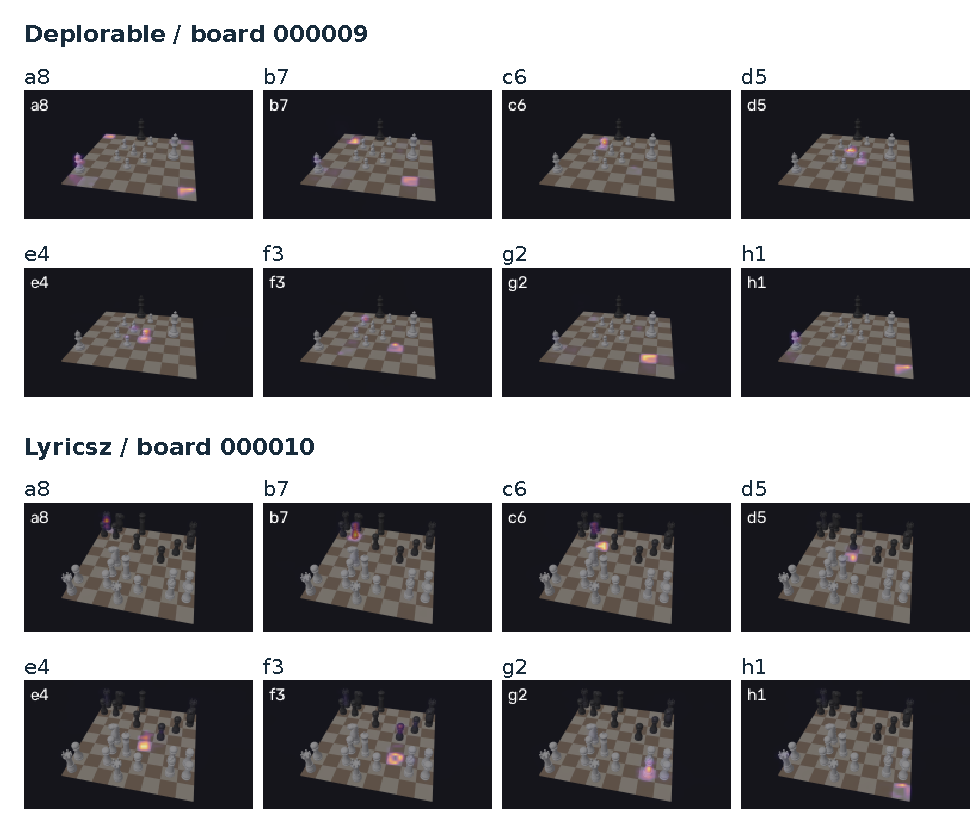
\includegraphics[width=\linewidth]{figures/attention_excerpt.pdf}
  \caption{Fixed, outcome-independent excerpt. Select the first two geometry names
  lexicographically in the frozen attention sample, then the lowest zero-padded
  board ID in each: Deplorable 000009 and Lyricsz 000010. For both boards use the
  same eight diagonal queries, a8, b7, c6, d5, e4, f3, g2 and h1. No prediction,
  correctness, confidence or attention magnitude enters this selection. Tiles are
  unchanged crops of the recorded overlays, normalized per query, not a shared
  saliency scale. The full set has 60 sheets (30 boards, 64 queries, two
  projections). Three sheets ship in the package, in \texttt{figures/attention/}.
  The full set is not released.}
  \label{fig:attention-excerpt}
\end{figure}


\FloatBarrier
\clearpage
\section{Receipt and test index}
\label{app:receipts}

The evidence index carries the digest of each copied file. Digests of the unredacted
originals are not shipped.
Table~\ref{tab:receipts} lists the completion receipts consumed by the generated tables
and figures, and the result summaries behind the Section~\ref{sec:lies} numbers (parity probe,
crop diagnostic, baseline and member scores, identifier-level holdout check, real-board check).
Per-image prediction files for those runs are not part of this package. A completion receipt records the checks stated by its own schema;
it is a checksummed record, not an independent attestation that no unrecorded
experiment occurred. It does not close the separate data, model, or asset
distribution gates.

\begingroup\small
\setlength{\tabcolsep}{4pt}
\begin{longtable}{>{\raggedright\arraybackslash}p{.49\linewidth}>{\raggedright\arraybackslash}p{.44\linewidth}}
\caption{Receipt and result-summary index. Paths and the hash of each copy are in the evidence index.}\label{tab:receipts}\\
\toprule
Receipt filename & % receipt: evidence/index.json; source: evidence/index.json; column definitions
Status / schema \\ % receipt: evidence/index.json; source: evidence/index.json; column definitions
\midrule

\endfirsthead
\toprule
Receipt filename & % receipt: evidence/index.json; source: evidence/index.json; column definitions
Status / schema \\ % receipt: evidence/index.json; source: evidence/index.json; column definitions
\midrule

\endhead
\bottomrule\endfoot
adaptation.complete.json & % receipt: evidence/index.json; source: evidence/index.json; benchmark_v2/adaptation.complete.json
schema\_\allowbreak{}v2\_\allowbreak{}frozen \\ % receipt: evidence/index.json; source: evidence/index.json; benchmark_v2/adaptation.complete.json

benchmark.complete.json & % receipt: evidence/index.json; source: evidence/index.json; benchmark_v2/benchmark.complete.json
schema\_\allowbreak{}v2\_\allowbreak{}frozen \\ % receipt: evidence/index.json; source: evidence/index.json; benchmark_v2/benchmark.complete.json

design.complete.json & % receipt: evidence/index.json; source: evidence/index.json; benchmark_v2/design.complete.json
design\_\allowbreak{}locked\_\allowbreak{}before\_\allowbreak{}rendering \\ % receipt: evidence/index.json; source: evidence/index.json; benchmark_v2/design.complete.json

exclusion\_\allowbreak{}audit.complete.json & % receipt: evidence/index.json; source: evidence/index.json; benchmark_v2/exclusion_audit.complete.json
all\_\allowbreak{}required\_\allowbreak{}sources\_\allowbreak{}audited \\ % receipt: evidence/index.json; source: evidence/index.json; benchmark_v2/exclusion_audit.complete.json

PARITY\_\allowbreak{}CONVENTIONS.complete.json & % receipt: evidence/index.json; source: evidence/index.json; docs/records/PARITY_CONVENTIONS.complete.json
parity-conventions-audit/v1 \\ % receipt: evidence/index.json; source: evidence/index.json; docs/records/PARITY_CONVENTIONS.complete.json

PHUONG\_\allowbreak{}LICENCE\_\allowbreak{}RECOVERY.complete.json & % receipt: evidence/index.json; source: evidence/index.json; docs/records/PHUONG_LICENCE_RECOVERY.complete.json
licence\_\allowbreak{}recovery\_\allowbreak{}complete\_\allowbreak{}version\_\allowbreak{}unresolved \\ % receipt: evidence/index.json; source: evidence/index.json; docs/records/PHUONG_LICENCE_RECOVERY.complete.json

PHUONG\_\allowbreak{}RELEASE\_\allowbreak{}STATUS\_\allowbreak{}2026-09-14.complete.json & % receipt: evidence/index.json; source: evidence/index.json; docs/records/PHUONG_RELEASE_STATUS_2026-09-14.complete.json
operator\_\allowbreak{}decision\_\allowbreak{}applied \\ % receipt: evidence/index.json; source: evidence/index.json; docs/records/PHUONG_RELEASE_STATUS_2026-09-14.complete.json

PHUONG\_\allowbreak{}RELEASE\_\allowbreak{}STATUS\_\allowbreak{}2026-09-15.complete.json & % receipt: evidence/index.json; source: evidence/index.json; docs/records/PHUONG_RELEASE_STATUS_2026-09-15.complete.json
author\_\allowbreak{}notice\_\allowbreak{}bindings\_\allowbreak{}updated \\ % receipt: evidence/index.json; source: evidence/index.json; docs/records/PHUONG_RELEASE_STATUS_2026-09-15.complete.json

PHUONG\_\allowbreak{}RELEASE\_\allowbreak{}STATUS\_\allowbreak{}2026-10-12.complete.json & % receipt: evidence/index.json; source: evidence/index.json; docs/records/PHUONG_RELEASE_STATUS_2026-10-12.complete.json
public\_\allowbreak{}doc\_\allowbreak{}notice\_\allowbreak{}bindings\_\allowbreak{}updated \\ % receipt: evidence/index.json; source: evidence/index.json; docs/records/PHUONG_RELEASE_STATUS_2026-10-12.complete.json

RELEASE\_\allowbreak{}LICENCE\_\allowbreak{}REVIEW.complete.json & % receipt: evidence/index.json; source: evidence/index.json; docs/records/RELEASE_LICENCE_REVIEW.complete.json
licence\_\allowbreak{}review\_\allowbreak{}complete\_\allowbreak{}with\_\allowbreak{}open\_\allowbreak{}release\_\allowbreak{}gates \\ % receipt: evidence/index.json; source: evidence/index.json; docs/records/RELEASE_LICENCE_REVIEW.complete.json

lora\_\allowbreak{}report.complete.json & % receipt: evidence/index.json; source: evidence/index.json; tools/reports/paper/lora_curve_2026-09-10/lora_report.complete.json
lora\_\allowbreak{}curve\_\allowbreak{}report\_\allowbreak{}complete \\ % receipt: evidence/index.json; source: evidence/index.json; tools/reports/paper/lora_curve_2026-09-10/lora_report.complete.json

result\_\allowbreak{}r1.complete.json & % receipt: evidence/index.json; source: evidence/index.json; tools/reports/paper/parity_probe_2026-09-09/result_r1.complete.json
completed\_\allowbreak{}exploratory\_\allowbreak{}probe \\ % receipt: evidence/index.json; source: evidence/index.json; tools/reports/paper/parity_probe_2026-09-09/result_r1.complete.json

precision\_\allowbreak{}results.complete.json & % receipt: evidence/index.json; source: evidence/index.json; tools/reports/paper/residual_shift_2026-09-10/diagnostics/precision_results.complete.json
c3\_\allowbreak{}precision\_\allowbreak{}probe\_\allowbreak{}complete \\ % receipt: evidence/index.json; source: evidence/index.json; tools/reports/paper/residual_shift_2026-09-10/diagnostics/precision_results.complete.json

overall\_\allowbreak{}recovery.complete.json & % receipt: evidence/index.json; source: evidence/index.json; tools/reports/paper/residual_shift_2026-09-10/overall_recovery.complete.json
complete\_\allowbreak{}after\_\allowbreak{}c3\_\allowbreak{}precision\_\allowbreak{}instrumentation\_\allowbreak{}recovery \\ % receipt: evidence/index.json; source: evidence/index.json; tools/reports/paper/residual_shift_2026-09-10/overall_recovery.complete.json

residual\_\allowbreak{}r1.complete.json & % receipt: evidence/index.json; source: evidence/index.json; tools/reports/paper/residual_shift_2026-09-10/r1/residual_r1.complete.json
c3\_\allowbreak{}residual\_\allowbreak{}complete \\ % receipt: evidence/index.json; source: evidence/index.json; tools/reports/paper/residual_shift_2026-09-10/r1/residual_r1.complete.json

timing.complete.json & % receipt: evidence/index.json; source: evidence/index.json; tools/reports/paper/timing_2026-09-10/timing.complete.json
c4\_\allowbreak{}timing\_\allowbreak{}complete \\ % receipt: evidence/index.json; source: evidence/index.json; tools/reports/paper/timing_2026-09-10/timing.complete.json

cq\_\allowbreak{}release.complete.json & % receipt: evidence/index.json; source: evidence/index.json; tools/reports/paper/timing_2026-09-10/timing.runs/cq_release.complete.json
c4\_\allowbreak{}timing\_\allowbreak{}complete \\ % receipt: evidence/index.json; source: evidence/index.json; tools/reports/paper/timing_2026-09-10/timing.runs/cq_release.complete.json

lora\_\allowbreak{}both\_\allowbreak{}n2000\_\allowbreak{}s303.complete.json & % receipt: evidence/index.json; source: evidence/index.json; tools/reports/paper/timing_2026-09-10/timing.runs/lora_both_n2000_s303.complete.json
c4\_\allowbreak{}timing\_\allowbreak{}complete \\ % receipt: evidence/index.json; source: evidence/index.json; tools/reports/paper/timing_2026-09-10/timing.runs/lora_both_n2000_s303.complete.json

lora\_\allowbreak{}both\_\allowbreak{}n2000\_\allowbreak{}s304.complete.json & % receipt: evidence/index.json; source: evidence/index.json; tools/reports/paper/timing_2026-09-10/timing.runs/lora_both_n2000_s304.complete.json
c4\_\allowbreak{}timing\_\allowbreak{}complete \\ % receipt: evidence/index.json; source: evidence/index.json; tools/reports/paper/timing_2026-09-10/timing.runs/lora_both_n2000_s304.complete.json

lora\_\allowbreak{}both\_\allowbreak{}n2000\_\allowbreak{}s305.complete.json & % receipt: evidence/index.json; source: evidence/index.json; tools/reports/paper/timing_2026-09-10/timing.runs/lora_both_n2000_s305.complete.json
c4\_\allowbreak{}timing\_\allowbreak{}complete \\ % receipt: evidence/index.json; source: evidence/index.json; tools/reports/paper/timing_2026-09-10/timing.runs/lora_both_n2000_s305.complete.json

lora\_\allowbreak{}both\_\allowbreak{}n500\_\allowbreak{}s303.complete.json & % receipt: evidence/index.json; source: evidence/index.json; tools/reports/paper/timing_2026-09-10/timing.runs/lora_both_n500_s303.complete.json
c4\_\allowbreak{}timing\_\allowbreak{}complete \\ % receipt: evidence/index.json; source: evidence/index.json; tools/reports/paper/timing_2026-09-10/timing.runs/lora_both_n500_s303.complete.json

lora\_\allowbreak{}both\_\allowbreak{}n8000\_\allowbreak{}s303.complete.json & % receipt: evidence/index.json; source: evidence/index.json; tools/reports/paper/timing_2026-09-10/timing.runs/lora_both_n8000_s303.complete.json
c4\_\allowbreak{}timing\_\allowbreak{}complete \\ % receipt: evidence/index.json; source: evidence/index.json; tools/reports/paper/timing_2026-09-10/timing.runs/lora_both_n8000_s303.complete.json

lora\_\allowbreak{}dark\_\allowbreak{}n2000\_\allowbreak{}s303.complete.json & % receipt: evidence/index.json; source: evidence/index.json; tools/reports/paper/timing_2026-09-10/timing.runs/lora_dark_n2000_s303.complete.json
c4\_\allowbreak{}timing\_\allowbreak{}complete \\ % receipt: evidence/index.json; source: evidence/index.json; tools/reports/paper/timing_2026-09-10/timing.runs/lora_dark_n2000_s303.complete.json

lora\_\allowbreak{}dark\_\allowbreak{}n2000\_\allowbreak{}s304.complete.json & % receipt: evidence/index.json; source: evidence/index.json; tools/reports/paper/timing_2026-09-10/timing.runs/lora_dark_n2000_s304.complete.json
c4\_\allowbreak{}timing\_\allowbreak{}complete \\ % receipt: evidence/index.json; source: evidence/index.json; tools/reports/paper/timing_2026-09-10/timing.runs/lora_dark_n2000_s304.complete.json

lora\_\allowbreak{}dark\_\allowbreak{}n2000\_\allowbreak{}s305.complete.json & % receipt: evidence/index.json; source: evidence/index.json; tools/reports/paper/timing_2026-09-10/timing.runs/lora_dark_n2000_s305.complete.json
c4\_\allowbreak{}timing\_\allowbreak{}complete \\ % receipt: evidence/index.json; source: evidence/index.json; tools/reports/paper/timing_2026-09-10/timing.runs/lora_dark_n2000_s305.complete.json

lora\_\allowbreak{}dark\_\allowbreak{}n500\_\allowbreak{}s303.complete.json & % receipt: evidence/index.json; source: evidence/index.json; tools/reports/paper/timing_2026-09-10/timing.runs/lora_dark_n500_s303.complete.json
c4\_\allowbreak{}timing\_\allowbreak{}complete \\ % receipt: evidence/index.json; source: evidence/index.json; tools/reports/paper/timing_2026-09-10/timing.runs/lora_dark_n500_s303.complete.json

lora\_\allowbreak{}dark\_\allowbreak{}n8000\_\allowbreak{}s303.complete.json & % receipt: evidence/index.json; source: evidence/index.json; tools/reports/paper/timing_2026-09-10/timing.runs/lora_dark_n8000_s303.complete.json
c4\_\allowbreak{}timing\_\allowbreak{}complete \\ % receipt: evidence/index.json; source: evidence/index.json; tools/reports/paper/timing_2026-09-10/timing.runs/lora_dark_n8000_s303.complete.json

private\_\allowbreak{}full.complete.json & % receipt: evidence/index.json; source: evidence/index.json; tools/reports/paper/timing_2026-09-10/timing.runs/private_full.complete.json
c4\_\allowbreak{}timing\_\allowbreak{}complete \\ % receipt: evidence/index.json; source: evidence/index.json; tools/reports/paper/timing_2026-09-10/timing.runs/private_full.complete.json

private\_\allowbreak{}raw.complete.json & % receipt: evidence/index.json; source: evidence/index.json; tools/reports/paper/timing_2026-09-10/timing.runs/private_raw.complete.json
c4\_\allowbreak{}timing\_\allowbreak{}complete \\ % receipt: evidence/index.json; source: evidence/index.json; tools/reports/paper/timing_2026-09-10/timing.runs/private_raw.complete.json

private\_\allowbreak{}warp\_\allowbreak{}high.complete.json & % receipt: evidence/index.json; source: evidence/index.json; tools/reports/paper/timing_2026-09-10/timing.runs/private_warp_high.complete.json
c4\_\allowbreak{}timing\_\allowbreak{}complete \\ % receipt: evidence/index.json; source: evidence/index.json; tools/reports/paper/timing_2026-09-10/timing.runs/private_warp_high.complete.json

private\_\allowbreak{}warp\_\allowbreak{}low.complete.json & % receipt: evidence/index.json; source: evidence/index.json; tools/reports/paper/timing_2026-09-10/timing.runs/private_warp_low.complete.json
c4\_\allowbreak{}timing\_\allowbreak{}complete \\ % receipt: evidence/index.json; source: evidence/index.json; tools/reports/paper/timing_2026-09-10/timing.runs/private_warp_low.complete.json

leak\_\allowbreak{}check\_\allowbreak{}render-host.json & % receipt: evidence/index.json; source: evidence/index.json; data/holdout/leak_check_render-host.json
result summary \\ % receipt: evidence/index.json; source: evidence/index.json; data/holdout/leak_check_render-host.json

cq\_\allowbreak{}baseline\_\allowbreak{}2026-09-08.json & % receipt: evidence/index.json; source: evidence/index.json; tools/reports/paper/cq_baseline_2026-09-08.json
result summary \\ % receipt: evidence/index.json; source: evidence/index.json; tools/reports/paper/cq_baseline_2026-09-08.json

cq\_\allowbreak{}baseline\_\allowbreak{}chesscog\_\allowbreak{}2026-09-08.json & % receipt: evidence/index.json; source: evidence/index.json; tools/reports/paper/cq_baseline_chesscog_2026-09-08.json
result summary \\ % receipt: evidence/index.json; source: evidence/index.json; tools/reports/paper/cq_baseline_chesscog_2026-09-08.json

cq\_\allowbreak{}baseline\_\allowbreak{}cvchess\_\allowbreak{}2026-09-08.json & % receipt: evidence/index.json; source: evidence/index.json; tools/reports/paper/cq_baseline_cvchess_2026-09-08.json
result summary \\ % receipt: evidence/index.json; source: evidence/index.json; tools/reports/paper/cq_baseline_cvchess_2026-09-08.json

crop\_\allowbreak{}diag\_\allowbreak{}2026-09-09.json & % receipt: evidence/index.json; source: evidence/index.json; tools/reports/paper/crop_diag_2026-09-09.json
result summary \\ % receipt: evidence/index.json; source: evidence/index.json; tools/reports/paper/crop_diag_2026-09-09.json

member\_\allowbreak{}cvchess\_\allowbreak{}full.tsv.json & % receipt: evidence/index.json; source: evidence/index.json; tools/reports/paper/member_cvchess_full.tsv.json
result summary \\ % receipt: evidence/index.json; source: evidence/index.json; tools/reports/paper/member_cvchess_full.tsv.json

member\_\allowbreak{}cvchess\_\allowbreak{}raw.tsv.json & % receipt: evidence/index.json; source: evidence/index.json; tools/reports/paper/member_cvchess_raw.tsv.json
result summary \\ % receipt: evidence/index.json; source: evidence/index.json; tools/reports/paper/member_cvchess_raw.tsv.json

member\_\allowbreak{}cvchess\_\allowbreak{}warp\_\allowbreak{}high.tsv.json & % receipt: evidence/index.json; source: evidence/index.json; tools/reports/paper/member_cvchess_warp_high.tsv.json
result summary \\ % receipt: evidence/index.json; source: evidence/index.json; tools/reports/paper/member_cvchess_warp_high.tsv.json

member\_\allowbreak{}cvchess\_\allowbreak{}warp\_\allowbreak{}low.tsv.json & % receipt: evidence/index.json; source: evidence/index.json; tools/reports/paper/member_cvchess_warp_low.tsv.json
result summary \\ % receipt: evidence/index.json; source: evidence/index.json; tools/reports/paper/member_cvchess_warp_low.tsv.json

member\_\allowbreak{}slcctest\_\allowbreak{}full.tsv.json & % receipt: evidence/index.json; source: evidence/index.json; tools/reports/paper/member_slcctest_full.tsv.json
result summary \\ % receipt: evidence/index.json; source: evidence/index.json; tools/reports/paper/member_slcctest_full.tsv.json

member\_\allowbreak{}slcctest\_\allowbreak{}raw.tsv.json & % receipt: evidence/index.json; source: evidence/index.json; tools/reports/paper/member_slcctest_raw.tsv.json
result summary \\ % receipt: evidence/index.json; source: evidence/index.json; tools/reports/paper/member_slcctest_raw.tsv.json

member\_\allowbreak{}slcctest\_\allowbreak{}warp\_\allowbreak{}high.tsv.json & % receipt: evidence/index.json; source: evidence/index.json; tools/reports/paper/member_slcctest_warp_high.tsv.json
result summary \\ % receipt: evidence/index.json; source: evidence/index.json; tools/reports/paper/member_slcctest_warp_high.tsv.json

member\_\allowbreak{}slcctest\_\allowbreak{}warp\_\allowbreak{}low.tsv.json & % receipt: evidence/index.json; source: evidence/index.json; tools/reports/paper/member_slcctest_warp_low.tsv.json
result summary \\ % receipt: evidence/index.json; source: evidence/index.json; tools/reports/paper/member_slcctest_warp_low.tsv.json

analysis.json & % receipt: evidence/index.json; source: evidence/index.json; tools/reports/paper/parity_probe_2026-09-09/analysis.json
result summary \\ % receipt: evidence/index.json; source: evidence/index.json; tools/reports/paper/parity_probe_2026-09-09/analysis.json

score\_\allowbreak{}cq\_\allowbreak{}cpu\_\allowbreak{}20261004.json & % receipt: evidence/index.json; source: evidence/index.json; tools/reports/paper/real_photo_2026-09-11/a1_light_2026-10-04/score_cq_cpu_20261004.json
result summary \\ % receipt: evidence/index.json; source: evidence/index.json; tools/reports/paper/real_photo_2026-09-11/a1_light_2026-10-04/score_cq_cpu_20261004.json

\end{longtable}
\endgroup


\subsection{Validation scope}
The paper build checks the complete cell matrix, deterministic table generation,
per-cell source comments, and rejection of altered evidence or broken historical
hash links. The export regressions separately test token boundaries, paired
original/export hashes, protected scene records, and explicit PDF decoder
failures. Passing these checks does not validate the scientific claims in the
paper text or resolve a distribution licence.

\subsection{Conditional localization diagnostic}
% receipt: evidence/tools/reports/paper/FREEZE_2026-09-09.json
Figure~\ref{fig:corners} retains the earlier detector summary as a separate
measurement from recognition. This figure and the historical pipeline comparison
use hash-pinned aggregate summaries without original run-completion receipts;
copying their hashes does not retrospectively certify the original runs. Error is normalized by the mean projected board
edge, and the figure reports excluded detections beside the elevation bands.
% historical source summary: evidence/tools/reports/paper/FREEZE_2026-09-09.json
\begin{figure}[htbp]
\centering
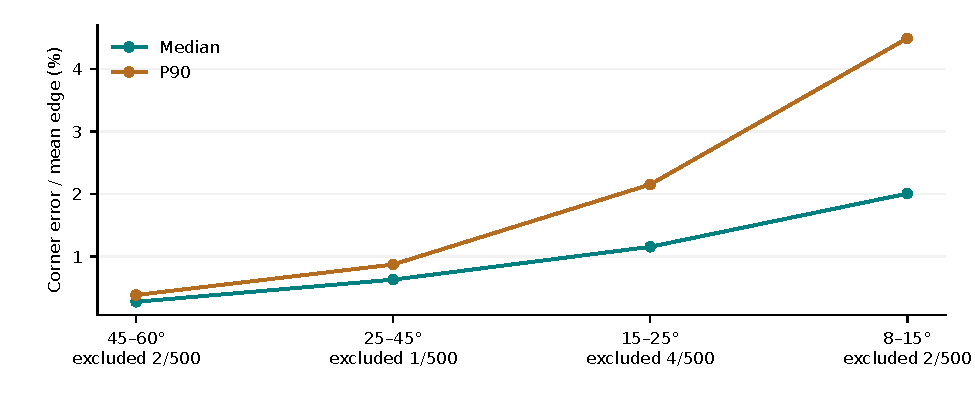
\includegraphics[width=\linewidth]{figures/corner_elevation.pdf}
\caption{Conditional corner error normalized by mean projected board edge. Excluded detections are reported for each elevation band. Historical aggregates are hash-pinned; original run-completion receipts are unavailable.}\label{fig:corners}
\end{figure}

